\documentclass[]{krantz}
\usepackage{lmodern}
\usepackage{amssymb,amsmath}
\usepackage{ifxetex,ifluatex}
\usepackage{fixltx2e} % provides \textsubscript
\ifnum 0\ifxetex 1\fi\ifluatex 1\fi=0 % if pdftex
  \usepackage[T1]{fontenc}
  \usepackage[utf8]{inputenc}
\else % if luatex or xelatex
  \ifxetex
    \usepackage{mathspec}
  \else
    \usepackage{fontspec}
  \fi
  \defaultfontfeatures{Ligatures=TeX,Scale=MatchLowercase}
\fi
% use upquote if available, for straight quotes in verbatim environments
\IfFileExists{upquote.sty}{\usepackage{upquote}}{}
% use microtype if available
\IfFileExists{microtype.sty}{%
\usepackage[]{microtype}
\UseMicrotypeSet[protrusion]{basicmath} % disable protrusion for tt fonts
}{}
\PassOptionsToPackage{hyphens}{url} % url is loaded by hyperref
\usepackage[unicode=true]{hyperref}
\PassOptionsToPackage{usenames,dvipsnames}{color} % color is loaded by hyperref
\hypersetup{
            pdftitle={Limitations of Interpretable Machine Learning Methods},
            colorlinks=true,
            linkcolor=Maroon,
            citecolor=Blue,
            urlcolor=Blue,
            breaklinks=true}
\urlstyle{same}  % don't use monospace font for urls
\usepackage{natbib}
\bibliographystyle{apalike}
\usepackage{color}
\usepackage{fancyvrb}
\newcommand{\VerbBar}{|}
\newcommand{\VERB}{\Verb[commandchars=\\\{\}]}
\DefineVerbatimEnvironment{Highlighting}{Verbatim}{commandchars=\\\{\}}
% Add ',fontsize=\small' for more characters per line
\usepackage{framed}
\definecolor{shadecolor}{RGB}{248,248,248}
\newenvironment{Shaded}{\begin{snugshade}}{\end{snugshade}}
\newcommand{\KeywordTok}[1]{\textcolor[rgb]{0.13,0.29,0.53}{\textbf{#1}}}
\newcommand{\DataTypeTok}[1]{\textcolor[rgb]{0.13,0.29,0.53}{#1}}
\newcommand{\DecValTok}[1]{\textcolor[rgb]{0.00,0.00,0.81}{#1}}
\newcommand{\BaseNTok}[1]{\textcolor[rgb]{0.00,0.00,0.81}{#1}}
\newcommand{\FloatTok}[1]{\textcolor[rgb]{0.00,0.00,0.81}{#1}}
\newcommand{\ConstantTok}[1]{\textcolor[rgb]{0.00,0.00,0.00}{#1}}
\newcommand{\CharTok}[1]{\textcolor[rgb]{0.31,0.60,0.02}{#1}}
\newcommand{\SpecialCharTok}[1]{\textcolor[rgb]{0.00,0.00,0.00}{#1}}
\newcommand{\StringTok}[1]{\textcolor[rgb]{0.31,0.60,0.02}{#1}}
\newcommand{\VerbatimStringTok}[1]{\textcolor[rgb]{0.31,0.60,0.02}{#1}}
\newcommand{\SpecialStringTok}[1]{\textcolor[rgb]{0.31,0.60,0.02}{#1}}
\newcommand{\ImportTok}[1]{#1}
\newcommand{\CommentTok}[1]{\textcolor[rgb]{0.56,0.35,0.01}{\textit{#1}}}
\newcommand{\DocumentationTok}[1]{\textcolor[rgb]{0.56,0.35,0.01}{\textbf{\textit{#1}}}}
\newcommand{\AnnotationTok}[1]{\textcolor[rgb]{0.56,0.35,0.01}{\textbf{\textit{#1}}}}
\newcommand{\CommentVarTok}[1]{\textcolor[rgb]{0.56,0.35,0.01}{\textbf{\textit{#1}}}}
\newcommand{\OtherTok}[1]{\textcolor[rgb]{0.56,0.35,0.01}{#1}}
\newcommand{\FunctionTok}[1]{\textcolor[rgb]{0.00,0.00,0.00}{#1}}
\newcommand{\VariableTok}[1]{\textcolor[rgb]{0.00,0.00,0.00}{#1}}
\newcommand{\ControlFlowTok}[1]{\textcolor[rgb]{0.13,0.29,0.53}{\textbf{#1}}}
\newcommand{\OperatorTok}[1]{\textcolor[rgb]{0.81,0.36,0.00}{\textbf{#1}}}
\newcommand{\BuiltInTok}[1]{#1}
\newcommand{\ExtensionTok}[1]{#1}
\newcommand{\PreprocessorTok}[1]{\textcolor[rgb]{0.56,0.35,0.01}{\textit{#1}}}
\newcommand{\AttributeTok}[1]{\textcolor[rgb]{0.77,0.63,0.00}{#1}}
\newcommand{\RegionMarkerTok}[1]{#1}
\newcommand{\InformationTok}[1]{\textcolor[rgb]{0.56,0.35,0.01}{\textbf{\textit{#1}}}}
\newcommand{\WarningTok}[1]{\textcolor[rgb]{0.56,0.35,0.01}{\textbf{\textit{#1}}}}
\newcommand{\AlertTok}[1]{\textcolor[rgb]{0.94,0.16,0.16}{#1}}
\newcommand{\ErrorTok}[1]{\textcolor[rgb]{0.64,0.00,0.00}{\textbf{#1}}}
\newcommand{\NormalTok}[1]{#1}
\usepackage{longtable,booktabs}
% Fix footnotes in tables (requires footnote package)
\IfFileExists{footnote.sty}{\usepackage{footnote}\makesavenoteenv{long table}}{}
\usepackage{graphicx,grffile}
\makeatletter
\def\maxwidth{\ifdim\Gin@nat@width>\linewidth\linewidth\else\Gin@nat@width\fi}
\def\maxheight{\ifdim\Gin@nat@height>\textheight\textheight\else\Gin@nat@height\fi}
\makeatother
% Scale images if necessary, so that they will not overflow the page
% margins by default, and it is still possible to overwrite the defaults
% using explicit options in \includegraphics[width, height, ...]{}
\setkeys{Gin}{width=\maxwidth,height=\maxheight,keepaspectratio}
\IfFileExists{parskip.sty}{%
\usepackage{parskip}
}{% else
\setlength{\parindent}{0pt}
\setlength{\parskip}{6pt plus 2pt minus 1pt}
}
\setlength{\emergencystretch}{3em}  % prevent overfull lines
\providecommand{\tightlist}{%
  \setlength{\itemsep}{0pt}\setlength{\parskip}{0pt}}
\setcounter{secnumdepth}{5}
% Redefines (sub)paragraphs to behave more like sections
\ifx\paragraph\undefined\else
\let\oldparagraph\paragraph
\renewcommand{\paragraph}[1]{\oldparagraph{#1}\mbox{}}
\fi
\ifx\subparagraph\undefined\else
\let\oldsubparagraph\subparagraph
\renewcommand{\subparagraph}[1]{\oldsubparagraph{#1}\mbox{}}
\fi

% set default figure placement to htbp
\makeatletter
\def\fps@figure{htbp}
\makeatother

\usepackage{booktabs}
\usepackage{longtable}
\usepackage[bf,singlelinecheck=off]{caption}

\usepackage{framed,color}
\definecolor{shadecolor}{RGB}{248,248,248}

\renewcommand{\textfraction}{0.05}
\renewcommand{\topfraction}{0.8}
\renewcommand{\bottomfraction}{0.8}
\renewcommand{\floatpagefraction}{0.75}

\renewenvironment{quote}{\begin{VF}}{\end{VF}}
\let\oldhref\href
\renewcommand{\href}[2]{#2\footnote{\url{#1}}}

\makeatletter
\newenvironment{kframe}{%
\medskip{}
\setlength{\fboxsep}{.8em}
 \def\at@end@of@kframe{}%
 \ifinner\ifhmode%
  \def\at@end@of@kframe{\end{minipage}}%
  \begin{minipage}{\columnwidth}%
 \fi\fi%
 \def\FrameCommand##1{\hskip\@totalleftmargin \hskip-\fboxsep
 \colorbox{shadecolor}{##1}\hskip-\fboxsep
     % There is no \\@totalrightmargin, so:
     \hskip-\linewidth \hskip-\@totalleftmargin \hskip\columnwidth}%
 \MakeFramed {\advance\hsize-\width
   \@totalleftmargin\z@ \linewidth\hsize
   \@setminipage}}%
 {\par\unskip\endMakeFramed%
 \at@end@of@kframe}
\makeatother


\usepackage{makeidx}
\makeindex

\urlstyle{tt}

\usepackage{amsthm}
\makeatletter
\def\thm@space@setup{%
  \thm@preskip=8pt plus 2pt minus 4pt
  \thm@postskip=\thm@preskip
}
\makeatother

\frontmatter

\title{Limitations of Interpretable Machine Learning Methods}
\author{}
\date{\vspace{-2.5em}2020-01-09}

\begin{document}
\maketitle

% you may need to leave a few empty pages before the dedication page

%\cleardoublepage\newpage\thispagestyle{empty}\null
%\cleardoublepage\newpage\thispagestyle{empty}\null
%\cleardoublepage\newpage
\thispagestyle{empty}

\begin{center}
\end{center}

\setlength{\abovedisplayskip}{-5pt}
\setlength{\abovedisplayshortskip}{-5pt}

{
\hypersetup{linkcolor=black}
\setcounter{tocdepth}{0}
\tableofcontents
}
\chapter*{Preface}\label{preface}


This book explains limitations of current methods in interpretable
machine learning. The methods include partial dependence plots (PDP),
Accumulated Local Effects (ALE), permutation feature importance,
leave-one-covariate out (LOCO) and local interpretable model-agnostic
explanations (LIME). All of those methods can be used to explain the
behavior and predictions of trained machine learning models. But the
interpretation methods might not work well in the following cases:

\begin{itemize}
\tightlist
\item
  if a model models interactions (e.g.~when a random forest is used)
\item
  if features strongly correlate with each other
\item
  if the model does not correctly model causal relationships
\item
  if parameters of the interpretation method are not set correctly
\end{itemize}

This book is the outcome of the seminar ``Limitations of Interpretable
Machine Learning'' which took place in summer 2019 at the Department of
Statistics, LMU Munich.

Cover by \href{https://twitter.com/YvonneDoinel}{@YvonneDoinel}

\begin{figure}
\centering

\includegraphics{images/by-nc-sa.png}
\caption{Creative Commons License}
\end{figure}

This book is licensed under the
\href{http://creativecommons.org/licenses/by-nc-sa/4.0/}{Creative
Commons Attribution-NonCommercial-ShareAlike 4.0 International License}.

\mainmatter

\chapter*{Foreword}\label{foreword}


\emph{Author: Christoph Molnar}

This book is the result of an experiment in university teaching. Each
semester, students of the Statistics Master can choose from a selection
of seminar topics. Usually, every student in the seminar chooses a
scientific paper, gives a talk about the paper and summarizes it in the
form of a seminar paper. The supervisors help the students, they listen
to the talks, read the seminar papers, grade the work and then \ldots{}
hide the seminar papers away in (digital) drawers. This seemed wasteful
to us, given the huge amount of effort the students usually invest in
seminars. An idea was born: Why not create a book with a website as the
outcome of the seminar? Something that will last at least a few years
after the end of the semester. In the summer term 2019, some Statistics
Master students signed up for our seminar entitled ``Limitations of
Interpretable Machine Learning''. When they came to the kick-off
meeting, they had no idea that they would write a book by the end of the
semester.

We were bound by the examination rules for conducting the seminar, but
otherwise we could deviate from the traditional format. We deviated in
several ways:

\begin{enumerate}
\def\labelenumi{\arabic{enumi}.}
\tightlist
\item
  Each student project is part of a book, and not an isolated seminar
  paper.
\item
  We gave challenges to the students, instead of papers. The challenge
  was to investigate a specific limitation of interpretable machine
  learning methods.
\item
  We designed the work to live beyond the seminar.
\item
  We emphasized collaboration. Students wrote some chapters in teams and
  reviewed each others texts.
\end{enumerate}

Looking back, the seminar was a lot of fun and -- from our perspective
-- successful. Especially considering that it was an experiment.
Everyone was highly motivated and we got great feedback from the
students that they liked the format. For the students it was a more work
than a traditional seminar. But in the end, our hope is that their
effort will pay off for them as well, not only because of their
increased visibility. It was also more work for us supervisors. But the
extra effort was worth it, since limitations of interpretability are
relevant for our research. For me the seminar was an inspiration. The
students had new ideas and new perspectives to approach the limitations
of interpretable machine learning.

\section*{Technical Setup}\label{technical-setup}


The book chapters are written in the Markdown language. The simulations,
data examples and visualizations were created with R \citep{rlang}. To
combine R-code and Markdown, we used rmarkdown. The book was compiled
with the bookdown package. We collaborated using git and github. For
details, head over to the
\href{https://github.com/compstat-lmu/iml_methods_limitations}{book's
repository}.

\chapter{Introduction}\label{introduction}

\emph{Author: Emanuel Renkl}

\emph{Supervisor: Christoph Molnar}

\section{Statistical Modeling: The Two
Approaches}\label{statistical-modeling-the-two-approaches}

In statistics, there are two approaches to reach conclusions from data
(see \citet{breiman2001}). First, the data modeling approach, where one
assumes that the data are generated by a given stochastic data model.
More specifically, a proposed model associates the input variables,
random noise and parameters with the response variables. Typical models
are for instance the linear and logistic regression model. These models
allow to predict what the responses are going to be to future input
variables and give information on how the response variables and input
variables are associated, i.e.~they are interpretable. Second, the
algorithmic modeling approach that uses algorithmic models and treats
the underlying data mechanism as unknown. More precisely, the goal is to
find an algorithm that operates on the input variables to predict the
response variables. Algorithms that are used are for instance random
forests and neural nets. These algorithms allow to predict what the
responses are going to be to future input variables, but do not give
information on how the response variables and input variables are
associated. Put differently, these algorithms produce black box models,
because they do not provide any direct explanation for their
predictions, i.e.~they are not interpretable.

Within the statistics community, the data modeling approach was
prevalently dominant for a long time (\citet{breiman2001}). However,
especially in the last decade the increasing availability of enormous
amounts of complex and unstructured data as well as the increase in
processing power of computers served as a breeding ground for a strong
shift to the algorithmic modeling approach, primarily for two reasons.\\
First, the data modeling approach is not applicable to exciting problems
like text, speech and image recognition (\citet{breiman2001}). Second,
for complex prediction problems new algorithms such as random forests
and neural nets outperform classical models in prediction accuracy as
they can model complex relationships in the data (\citet{breiman2001}).
For these reasons, more and more researchers switched from the data
modeling approach to the algorithmic modeling approach that is much more
common under the name machine learning.

But what about interpretability? As we learned in the first paragraph
machine learning algorithms are black box models that do not provide any
direct explanation for their predictions. Hence, the questions arises
whether we need to know why an algorithm makes a certain prediction? To
get a better feeling for this question, it's helpful to understand how
algorithms learn to make predictions and for which tasks machine
learning is used.

\section{Importance of
Interpretability}\label{importance-of-interpretability}

Algorithms learn to make predictions from training data. Thus,
algorithms also pick up biases of the training data and hence may not be
robust under certain circumstances, e.g.~they perform well on a test
set, but not in the real world. Such behavior can lead to undesired
outcomes.\\
For instance, consider a simple husky versus wolf classifier that
misclassifies some huskies as wolves (see \citet{ribeiro2016should}).
Since the machine learning model does not give any information on how
the response and input variables are associated, we do not know why it
classified a husky as a wolf. However, interpretability might be useful
to debug the algorithm and see if this problem is persistent or not.
Using methods that make machine learning algorithms interpretable and
that we will discuss later in the book, we would find that the
misclassification was due to the snow on the image. The algorithm
learned to use snow as a feature for classifying images as wolves. This
might make sense in the training dataset, but not in the real world.
Thus, in this example interpretability helps us to understand how the
algorithm gets to the result and hence, we know in which cases the
robustness of the algorithm is not given. In the following, we want to
derive the importance of interpretability by focusing on academic and
industrial settings.

Broadly speaking in academia machine learning is used to draw
conclusions from data. However, off the shelf machine learning
algorithms only give predictions without explanations. Thus, they answer
only the ``what'', but not the ``why'' of a certain question and hence,
do not allow for actual scientific findings. Especially, in areas such
as life sciences and social sciences, that aim to identify causal
relationships between input and response variables interpretability is
key to scientific discoveries.\\
For example, in a medical study researchers applying machine learning
found that patients with pneumonia who have a history of asthma have a
lower risk of dying from pneumonia than the general population
(\citet{caruana2015intelligible}). This is of course counterintuitive.
However it was a true pattern in the training data: pneumonia patients
with a history of asthma were usually admitted not only to the hospital
but also directly to the Intensive Care Unit. The aggressive care
received by asthmatic pneumonia patients was so effective that it
lowered their risk of dying from pneumonia compared to the general
population. However, since the prognosis for these patients was above
average, models trained on this data erroneously find that asthma
reduces the risk, while asthmatics actually have a much higher risk if
they are not hospitalized. Hence, in this example blind trust in the
machine learning algorithm would yield misleading results. Thus,
interpretability is necessary in research to help identify causal
relationships and increase the reliability and robustness of machine
learning algorithms. Especially in areas outside of statistics the
adoption of machine learning would be facilitated by making these models
interpretable by adding explanations to their predictions.

In industry, machine learning is a standard component of almost any
digital product offered by the big tech companies. From Amazons Alexa,
or Netflixs movie recommendation system to the search algorithm from
Google and Facebooks feed. These companies use machine learning to
improve their products and business models. However, their machine
learning algorithms are also built on training data collected from their
users. Thus, in the age af data leaks à la Cambridge Analytica people
want to understand for what purposes their data is collected and how the
algorithms work that keep them on the streaming platforms or urge them
to buy additional products and spend more time on social media.\\
Thus, in the digital world, interpretability of machine learning models
would yield to a broader understanding of machine learning in the
society and make the technology more trustworthy and fair. Switching to
the analog world we see a far slower adoption of machine learning
sytsems at scale. This is due to the fact that decisions made by machine
learning systems in the real world can have far more severe consequences
than in the digital world.\\
For instance, if the wrong movie is suggested to us it really doesn't
matter, but if a machine learning system that is deployed to a self
driving car does not recognize a cyclist it might take the wrong
decision with real lifes at stake (see \citet{molnar2019}). We need to
be sure that the machine learning system is flawless, because driving
over a cyclist is pretty bad. For example, an explanation might show
that the most important feature is to recognize the two wheels of a
bicycle, and this explanation helps you to think about certain edge
cases, such as bicycles with side pockets that partially cover the
wheels. Self-driving cars are just one example where machines are taking
over decisions in the real world that were previously taken by humans
and can involve severe and sometimes irreversible consequences.
Interpretability helps to ensure the reliability and robusntess of these
systems and thus makes them safer.

To conclude, adding interpretability to machine learning algorithms is
necessary in both academic and industrial applications. While we
distinguished between academia and industry settings, the general
points, causality, robustness \& reliability, trust and fairness are of
course valid in both worlds.\\
However, for academia, interpretability is especially key to identify
causal relationships and increase the reliability and robustness of
scientific discoveries made by the help of machine learning
algorithms.\\
In industrial settings establishing trust in and fairness of machine
learning systems matters most in low-risk environments whereas
robustness and reliability is key to high-risk environments where
machines take over decisions that have far reaching consequences.

Now that we established the importance of interpretability, how do we
put this into practice? A restriction to machine learning models that
are considered interpretable due to their simple structure, such as
short decision trees or sparse linear models has the drawback that
better performing models are excluded a priori from model selection.
Hence, do we trade of prediction versus information and go back to more
simple models? - No!\\
We seperate the explanations from the machine learning model and apply
interpretable methods that analyze the model after the model is trained.

\section{Interpretable Machine
Learning}\label{interpretable-machine-learning}

As discussed in the previous chapter, most machine learning algorithms
produce black box models, because they do not provide any direct
explanation for their predictions. However, we do not want to restrict
ourselves to models that are considered interpretable due to their
simple structure and thus trade prediction accuracy for
interpretability. Instead, we make machine learning models interpretable
by applying methods that analyze the model after the model is trained,
i.e.~we establish post-hoc interpretability. Moreover, we are separating
the explanations from the machine learning model, i.e we focus on so
called model-agnostic interpretation methods.\\
Post-hoc, model-agnostic explanation systems have several advantages
(\citet{ribeiro2016model}). First, since we seperate the underlying
machine learning model and its interpretation, developers can work with
any model as the interpretation method is independent of the model. Thus
we establish model flexibility. Second, since the interpretation is
independent of the underlying machine learning model, the form of the
interpretation also becomes independent. For instance in some cases it
might be useful to have a linear formula, in other cases a graphic with
feature importances is more appropriate. Thus, we establish explanation
flexibility.

So what do these explanation systems do? - As discussed before,
interpretation methods for machine learning algorithms ensure causal
relationships, robustness \& reliability and establish trust and
fairness. More specifically, they do so by shedding light on the
following issues (see \citet{molnar2019}):

\begin{itemize}
\tightlist
\item
  Algorithm transparency - How does the algorithm create the model?
\item
  Global, kolistic model interpretability - How does the trained model
  make predictions?
\item
  Global model interpretability on a modular level - How do parts of the
  model affect predictions?
\item
  Local interpretability for a single prediction - Why did the model
  make a certain prediction for an instance?
\item
  Local interpretability for a group of predictions - Why did the model
  make specific predictions for a group of instances?
\end{itemize}

Now that we learned that post-hoc and model-agnostic methods ensure
model as well as explanantion flexibility and in which ways explanation
systems ensure causal relationships, robustness \& reliability and
establish trust and fairness, we can move on to the outline of the
booklet and discuss specific interpretation methods and their
limitations.

\section{Outline of the booklet}\label{outline-of-the-booklet}

This booklet introduces and investigates the limitations of current
post-hoc and model agnostic approaches in interpretable machine
learning, such as Partial Dependence Plots (PDP), Accumulated Local
Effects (ALE), Permutation Feature Importance (PMI), Leave-One-Covariate
Out (LOCO) and Local Interpretable Model-Agnostic Explanations (LIME).
All of these methods can be used to explain the behavior and predictions
of trained machine learning models. However, their reliability and
compactness deteriorate when models use a high number of features, have
strong feature interactions and complex feature main effects among
others. In the following, the methods mentioned are introduced and the
outline of the booklet is given.

To start with, PDP and ALE are methods that enable a better
understanding of the relationship between the outcome and feature
variables of a machine learning model. Common to both methods is that
they reduce the prediction function to a function that depends on only
one or two features (\citet{molnar2019}). Both methods reduce the
function by averaging the effects of the other features, but they differ
in how the averages are calculated.\\
PDP, for example, visualizes whether the relationship between the
outcome and a feature variable is, for instance, linear, monotonic or
nonlinear and hence allows for a straightforward interpretation of the
marginal effect of a certain feature on the predicted outcome of a model
(\citet{friedman2001greedy}). However, this holds only true as long as
the feature in question is not correlated with any other features of the
model. ALE plots are basically a faster and unbiased alternative to PDP,
because they can interpret models containing correlated variables
correctly (\citet{molnar2019}). Chapter \ref{pdp} of the booklet gives a
short introduction to PDP. Next, PDP and its limitations when features
are correlated are investigated in Chapter \ref{pdp-correlated},
respectively. Chapter \ref{pdp-causal} discusses if PDP allow for causal
interpretations. Chapter \ref{ale} gives then a short introduction to
ALE. ALE and PDP are compared in detail in Chapter \ref{ale-pdp}. The
choice of intervals, problems with pice-wise constant models and
categorial features in the context of ALE are investigated in Chapter
\ref{ale-misc}.

Yet, PDP and ALE do not provide any insights to what extent a feature
contributes to the predictive power of a model - in the following
defined as feature importance. PFI and LOCO are two methods that allow
us to compute and visualize the importance of a certain feature for a
machine learning model. PFI by \citet{breiman2001random} measures the
importance of a feature by calculating the increase in the model's
prediction error after permuting the feature. Leave-One-Covariate-Out
(LOCO) by \citet{lei2018distribution}, requires to refit the model as
the approach is based on leaving features out instead of permuting them
(\citet{casalicchio2018visualizing}). Chapter \ref{pfi} gives a short
introduction to PFI and LOCO and gives rise to its limitations. Chapter
\ref{pfi-correlated} discusses both methods in the case of correlated
features. Then partial and individual PFI are discussed in Chapter
\ref{pfi-partial} and the issue whether feature importance should be
computed on training or test data is discussed in Chapter
\ref{pfi-data}.

Finally, LIME is a method that explains individual predictions of a
black box machine learning model by locally approximating the prediction
using a less complex and interpretable model (\citet{molnar2019}). These
simplifying models are referred to as surrogate models. Consider for
instance a neural network that is used for a classification task. The
neural network itself is of course not interpretable, but certain
decision boundaries could, for example, be explained reasonably well by
a logistic regression which in fact yields interpretable coefficients.
To refer to the first paragraph of the introduction, we use the data
modeling approach to explain the algorithmic modeling approach in this
example. Chapter \ref{lime} gives a short introduction to LIME. Chapter
\ref{lime-neighbor} sheds light on the effect of the neighbourhood on
LIME's explanantion for tabular data. Chapter \ref{lime-sample} deals
with the sampling step in LIME and the resulting side effects in terms
of feature weight stability of the surrogate model.

Now that we shortly introduced the different methods we can move to the
respective chapters of the booklet which discuss the methods and their
limitations in more detail and by the help of practical examples.

\chapter{Introduction to Partial Dependence Plots (PDP) and Individual
Conditional Expectation (ICE)}\label{pdp}

\emph{Authors: Thommy Dassen, Naiwen Hou, Veronika Kronseder}

\emph{Supervisor: Gunnar König}

\section{Partial Dependence Plots
(PDP)}\label{partial-dependence-plots-pdp}

The Partial Dependence Plot (PDP) is a rather intuitive and
easy-to-understand visualization of the features' impact on the
predicted outcome. If the assumptions for the PDP are met, it can show
the way a feature impacts an outcome variable. More precisely, mapping
the marginal effect of the selected variable(s) uncovers the linear,
monotonic or nonlinear relationship between the predicted response and
the individual feature variable(s) \citep{molnar2019}.

The underlying function can be described as follows:

Let \(x_S\) be the set of features of interest for the PDP and \(x_C\)
the complement set which contains all other features. While the general
model function \(f(x) = f(x_S, x_C)\) depends on all input variables,
the partial dependence function marginalizes over the feature
distribution in set C \citep{hastie2013elements}:

\[f_{x_S}(x_S) = \mathbb{E}_{x_C}[f(x_S, x_C)]\]

The partial dependence function can be estimated by averaging
predictions with actual feature values of \(x_C\) in the training data
at given values of \(x_S\) or, in other words, it computes the marginal
effect of \(x_S\) on the prediction. In order to obtain realistic
results, a major assumption of the PDP is that the features in \(x_S\)
and \(x_C\) are independent and thus
uncorrelated.\citep{hastie2013elements}

\[\hat{f}_{x_S}(x_S)=\frac{1}{n}\sum_{i=1}^{n}f(x_S, x^{(i)}_{C})\]

An example of a PDP based on the `Titanic' data set, which contains
information on the fate of 2224 passengers and crew members during the
Titanic's maiden voyage, is given in figure \ref{fig:plot1}.

\begin{figure}

{\centering 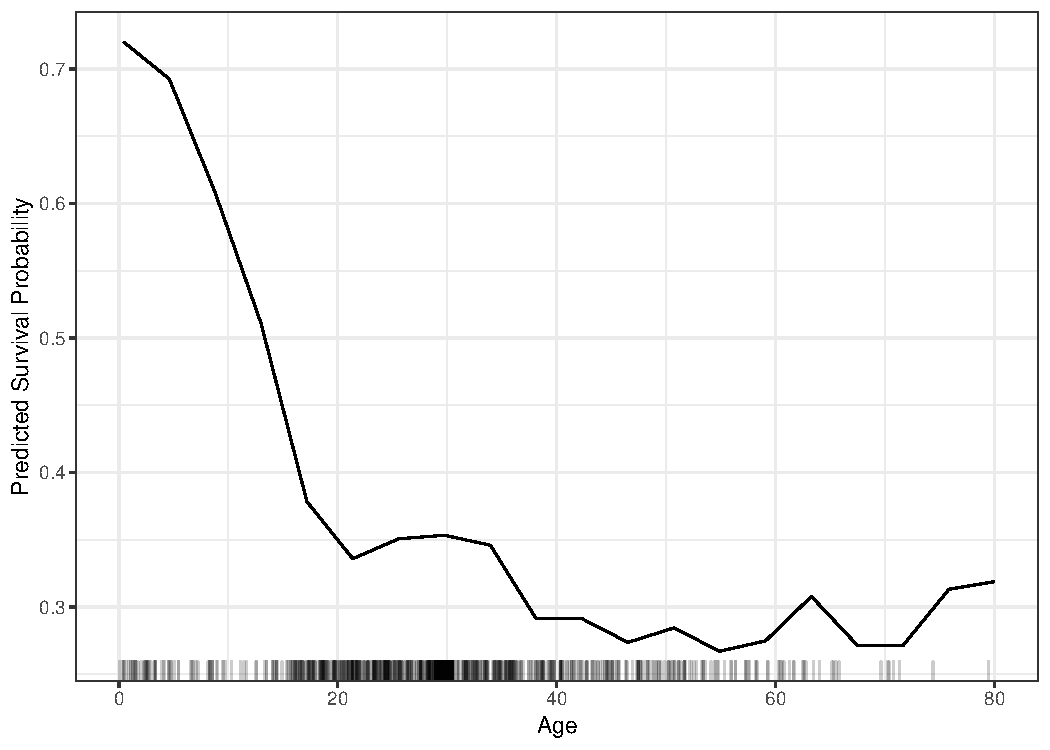
\includegraphics[width=0.8\linewidth]{images/PDP_Plot_1} 

}

\caption{PDP for predicted survival probability and numeric feature variable 'Age'. The probability to survive sharply drops at a young age and more moderately afterwards. The rug on the x-axis illustrates the distribution of observed training data.}\label{fig:plot1}
\end{figure}

When a feature is categorical, rather than continuous, the partial
dependence function is modeled separately for all of the K different
classes of said feature. It maps the predictions for each respective
class at given feature values of \(x_S\) \citep{hastie2013elements}.

For such categorical features, the partial dependence function and the
resulting plot are produced by replacing all observed \(x_S\)-values
with the respective category and averaging the predictions. This
procedure is repeated for each of the features' categories
\citep{molnar2019}. As an example, figure \ref{fig:plot2} shows the
partial dependence for the survival probability prediction for
passengers on the Titanic and the categorical feature `passenger class'.

\begin{figure}

{\centering 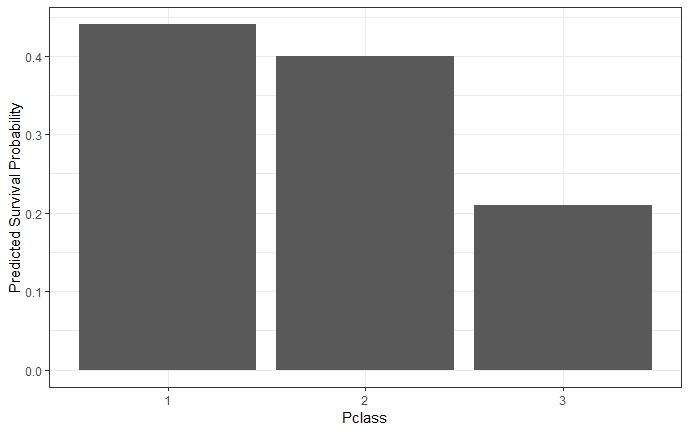
\includegraphics[width=0.8\linewidth]{images/PDP_Plot_2} 

}

\caption{The PDP for survival probability and categorical feature ' passenger class' reveals that passengers in lower classes had a lower probability to survive than those in a higher class.}\label{fig:plot2}
\end{figure}

\subsection{Advantages and Limitations of Partial Dependence
Plots}\label{advantages-and-limitations-of-partial-dependence-plots}

Partial Dependence Plots are easy to compute and a popular way to
explain insights from black box Machine Learning models. With their
intuitive character, PDPs are perfect for communicating to a
non-technical audience. However, due to limited visualization techniques
and the restriction of human perception to a maximum of three
dimensions, only one or two features can reasonably be displayed in one
PDP \citep{molnar2019}. \ref{fig:plot3} shows that the combination of
one numerical (Age) and one categorical (Sex) feature still allows
rather precise interpretation. The combination of two numerical features
(Age \& Fare) still works, but already degrades the interpretability
with its colour intensity scale as shown in figure \ref{fig:plot4}.

\begin{figure}

{\centering 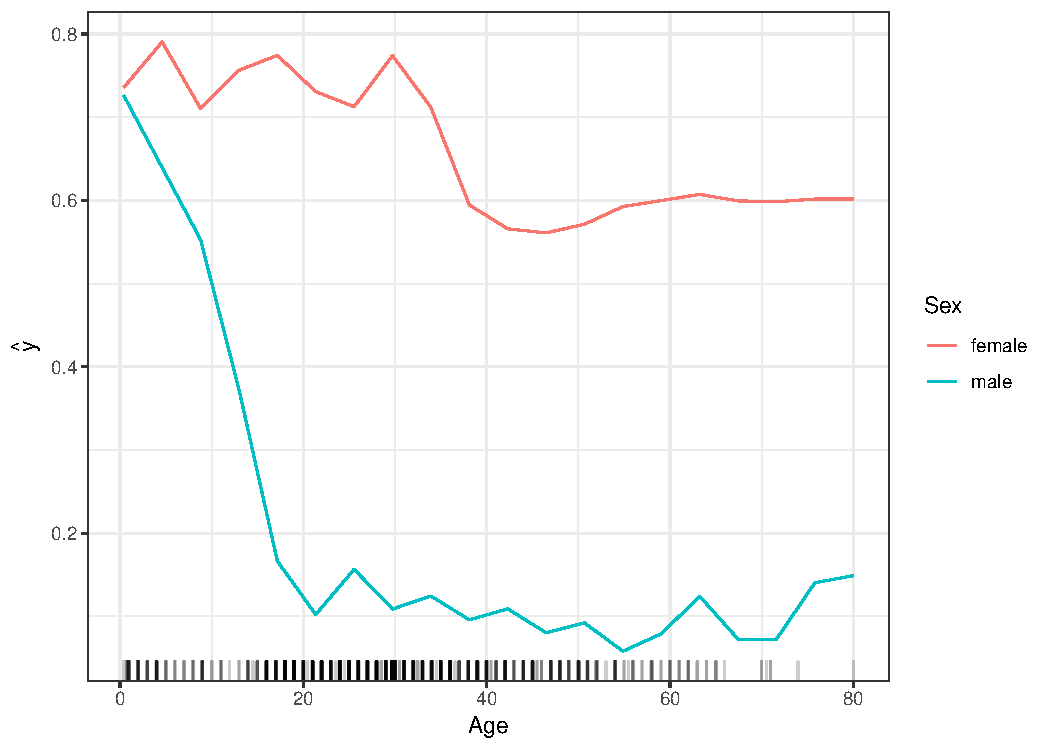
\includegraphics[width=0.8\linewidth]{images/PDP_Plot_3} 

}

\caption{Two-dimensional PDP for predicted survival probability and numerical feature 'Age', together with the categorical feature 'Sex'. The PDP shows that while the survival probability for both genders declines as age increases, there is a difference between genders. It is clear that the decrease is much steeper for males.}\label{fig:plot3}
\end{figure}

\begin{figure}

{\centering 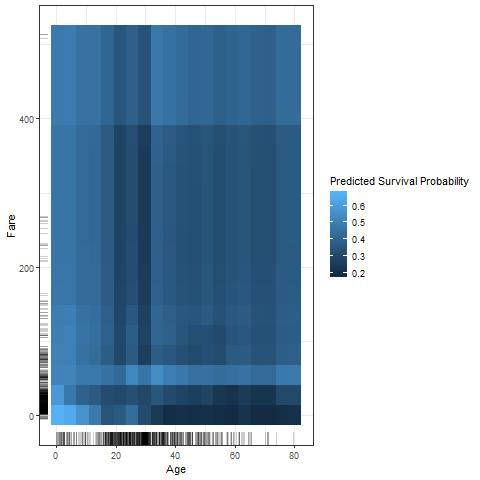
\includegraphics[width=0.8\linewidth]{images/PDP_Plot_4} 

}

\caption{Two-dimensional PDP for predicted survival probability and numerical features 'Age' and 'Fare'. The PDP illustrates that the survival probability of younger passengers is fairly uniform for varying fares, while adults travelling at a lower fare also had a much lower probability to survive compared to those that paid a high fare.}\label{fig:plot4}
\end{figure}

Drawing a PDP with one or two feature variables allows a
straight-forward interpretation of the marginal effects. This holds true
as long as the features are not correlated. Should this independence
assumption be violated, the partial dependence function will produce
unrealistic data points. For instance, a correlation between height and
weight leading to a data point for someone taller than 2 meters weighing
less than 50 kilos. Furthermore, opposite effects of heterogeneous
subgroups might remain hidden through averaging the marginal effects,
which could lead to wrong conclusions \citep{molnar2019}.

\section{Individual Conditional Expectation
Curves}\label{individual-conditional-expectation-curves}

While partial dependence plots provide the average effect of a feature,
Individual Conditional Expectation (ICE) plots are a method to
disaggregate these averages. ICE plots visualize the functional
relationship between the predicted response and the feature separately
for each instance. In other words, a PDP averages the individual lines
of an ICE plot \citep{molnar2019}.

More formally, ICE plots can be derived by considering the estimated
response function \(\hat{f}\) and the observations
\({(x^{(i)}_S, x^{(i)}_C)}^N_{i=1}\). The curve \(\hat{f}_S^{(i)}\) is
plotted against the observed values of \(x^{(i)}_S\) for each of the
observed instances while \(x^{(i)}_C\) remains fixed at each point on
the x-axis \citep{molnar2019, Goldstein2013}

As shown in figure \ref{fig:plot5}, each line represents one instance
and visualizes the effect of varying the feature value \(x^{(i)}_S\)
(Age) of a particular instance on the model's prediction, given all
other features remain constant (c.p.). An ICE plot can highlight the
variation in the fitted values across the range of a feature. This
suggests where and to what extent heterogeneities might exist.

\begin{figure}

{\centering 
\includegraphics[width=0.8\linewidth]{images/PDP_Plot_5} 

}

\caption{ICE plot of survival probability by Age. The yellow line represents the average of the individual lines and is thus equivalent to the respective PDP. The individual conditional relationships indicate that there might be underlying heterogeneity in the complement set.}\label{fig:plot5}
\end{figure}

\subsection{Centered ICE Plot}\label{centered-ice-plot}

If the curves of an ICE plot are stacked or have a wide range of
intercepts it can be difficult to observe heterogeneity in the model.
The so-called centered ICE plot (c-ICE plot) is a simple solution to
this problem. The curves are centered at a certain point in the feature
and display only the difference in the prediction to this point
\citep{molnar2019}. After anchoring a location \(x^a\) in the range of
\(x_s\) and connecting all prediction lines at that point, the new
curves are defined as:

\[\hat{f}^{(i)}_{cent} = \hat{f^{(i)}} - \mathbf{1}\hat{f}(x^a,x^{(i)}_C)\]
Experience has shown that the most interpretable plots occur when the
anchor point \(x^a\) is chosen as minimum or maximum of the observed
values. Figure \ref{fig:plot6} shows the effect of centering the ICE
curves of survival probability by Age at the minimum of observed ages in
the `Titanic' data set.

\begin{figure}

{\centering 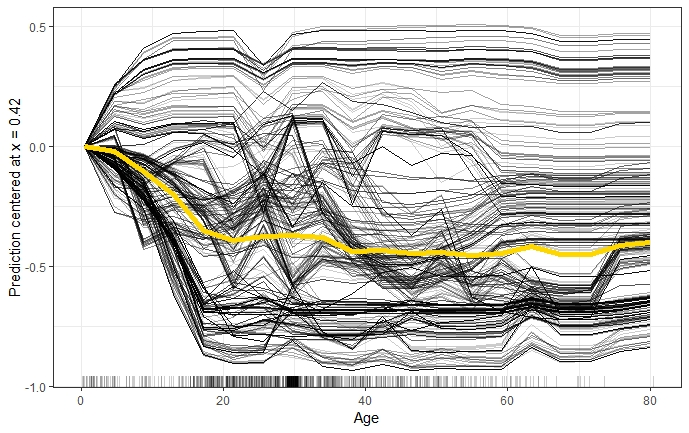
\includegraphics[width=0.8\linewidth]{images/PDP_Plot_6} 

}

\caption{Centered ICE plot of survival probability by Age. All lines are fixed to 0 at the minimum observed age of 0.42. The y-axis shows the survival probability difference to age 0.42. Centrered ICE plot shows that compared to age 0.42, the predictions for most passengers decrease as age increases. However, there are quite a few passengers with opposite predictions.}\label{fig:plot6}
\end{figure}

\subsection{Derivative ICE Plot}\label{derivative-ice-plot}

Another way to explore the heterogeneity is to show plots of the partial
derivative of \(\hat{f}\) with respect to \(x_s\). Assume that \(x_s\)
does not interact with the other predictors in the fitted model, the
prediction function can be written as:

\[\hat{f}(x) = \hat{f}(x_s,x_C) = g(x_s) + h(x_C),\]

so that \[\frac{\partial{\hat{f}(\mathbf{x})}}{\partial x_s} = g'(x_s)\]

When no interactions are present in the fitted model, all curves in the
d-ICE plot are equivalent and the plot shows a single line. When
interactions do exist, the derivative lines will be heterogeneous. As it
can be difficult to visually assess derivatives from ICE plots, it is
useful to plot an estimate of the partial derivative directly
\citep{Goldstein2013}.

\subsection{Advantages and Limitations of ICE
Plots}\label{advantages-and-limitations-of-ice-plots}

The major advantage of ICE plots is that they are even more intuitive
than PDPs which enables data scientists to drill much deeper to explore
individual differences. This may help to identify subgroups and
interactions between model inputs. However, there are also some
disadvantages of ICE plots. Firstly, only one feature can be plotted in
an ICE plot meaningfully. Otherwise, there would be a problem of
overplotting and it would be hard to distinguish anything in the plot.
Secondly, just like PDPs, ICE plots for correlated features may produce
invalid data points. Finally, without additionally plotting the PDP it
might be difficult to see the average in ICE plots \citep{molnar2019}.

\chapter{PDP and Correlated Features}\label{pdp-correlated}

\emph{Author: Veronika Kronseder}

\emph{Supervisor: Giuseppe Casalicchio}

\section{Problem Description}\label{ProblemDescription}

As outlined in chapter 2, PDPs and ICE plots are meaningful graphical
tools to visualize the impact of individual feature variables. This is
particularly true for black box algorithms, where the mechanism of each
feature and its influence on the generated predictions may be difficult
to retrace \citep{Goldstein2013}.

The reliability of the produced curves, however, strongly builds on the
independence assumption of the features. Furthermore, results can be
misleading in areas with no or little observations, where the curve is
drawn as a result of extrapolation. In this chapter, we want to
illustrate and discuss the issue of dependencies between different types
of variables, missing values and the associated implications on PDPs.

\subsection{What is the issue with dependent
features?}\label{what-is-the-issue-with-dependent-features}

When looking at PDPs, one should bear in mind that by definition the
partial dependence function does not reflect the isolated effect of
\(x_S\) while the features in \(x_C\) are ignored. This approach would
correspond to the conditional expectation
\(\tilde{f}_S(x_S) = \mathbb{E}_{x_C}[f(x_S, x_C)|x_S]\), which is only
congruent to the partial dependence function
\(f_{x_S}(x_S) = \mathbb{E}_{x_C}[f(x_S, x_C)]\) in case of \(x_S\) and
\(x_C\) being independent \citep{hastie2013elements}.

Although unlikely in many practical applications, the independence of
feature variables is one of the major assumptions to produce meaningful
PDPs. Its violation would mean that, by calculating averages of the
features in \(x_C\), the estimated partial dependence function
\(\hat{f}_{x_S}(x_S)\) takes unrealistic data points into consideration
\citep{molnar2019}.

Figure \ref{fig:Figure01} illustrates the problem by contrasting
simulated data with independent features \(x_1\) and \(x_2\) on the left
with an example where the two features have a strong linear dependency,
and thus are highly correlated, on the right.

\begin{figure}
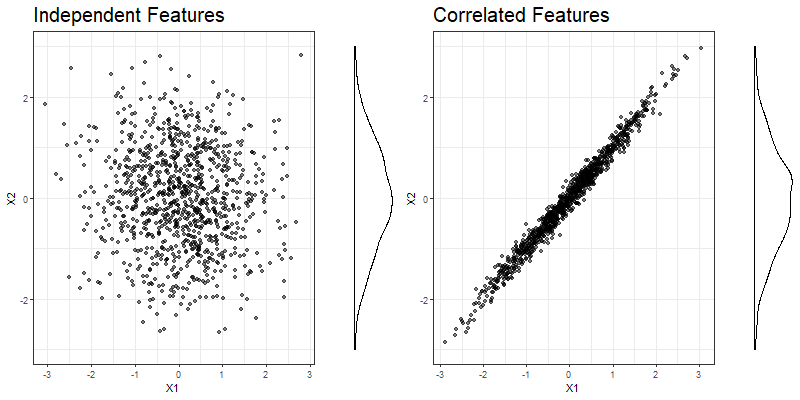
\includegraphics[width=1\linewidth]{images/VK_PDP_1_Data_ind_dep} \caption{Simulated data for independent (left) and strongly correlated (right) features $x_1$ and $x_2$. The marginal distribution of $x_2$ is displayed on the right side of each plot.}\label{fig:Figure01}
\end{figure}

When computing the PDP for feature \(x_1\), we take \(x_2\) into account
by calculating the mean predictions at observed \(x_2\) values in the
training data, while the values of \(x_1\) are given. This makes sense
in the independent case, where observations are randomly scattered.
However, when looking at the correlated features in the right part of
figure \ref{fig:Figure01}, the average is not a realistic value in
combination with certain values of \(x_1\), e.g.~in the very left and
the very right part of the feature distribution.

\subsection{What is the issue with
extrapolation?}\label{what-is-the-issue-with-extrapolation}

Generally speaking, extrapolation means leaving the distribution of
observed data. On the one hand, this can affect the predictions, namely
in the event of the prediction function doing `weird stuff' in
unobserved areas. In chapter \ref{ExtrapolationProblem} we will see an
example where this instant leads to a failure of the PDP
\citep{molnar2019}.

On the other hand, PDPs are also directly exposed to extrapolation
problems due to the fact that the estimated partial dependence function
\(\hat{f}_{x_S}\) is evaluated at each observed \(x^{(i)}_{S}\), giving
a set of N ordered pairs:
\(\{(x^{(i)}_{S}, \hat{f}_{x^{(i)}_{S}})\}_{i=1}^N\). The resulting
coordinates are plotted against each other and joined by lines. Not only
outside the margins of observed values, but also in areas with a larger
distance between neighboured \(x_S\) values, the indicated relationship
with the target variable might be inappropriate and volatile in case of
outliers \citep{Goldstein2013}.

In figure \ref{fig:Figure02}, a part of the previously simulated
observations has been deleted from both the independent and the
correlated example to visualize a data situation which might have an
impact on the PDP in terms of extrapolation. An example is given in
chapter \ref{ExtrapolationProblemEstablished}. The shift in observed
areas can also be noticed from the marginal distribution of \(x_2\).

\begin{figure}
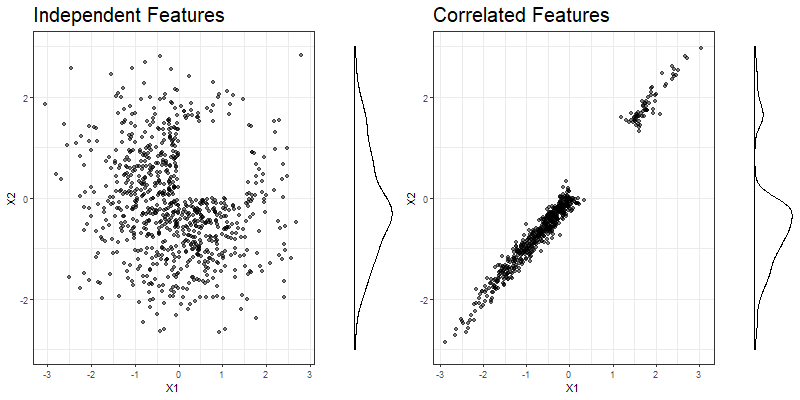
\includegraphics[width=1\linewidth]{images/VK_PDP_2_Data_ind_dep_gap} \caption{Manipulated simulated data for independent (left) and strongly correlated (right) features $x_1$ and $x_2$. Observations where both the value of $x_1$ and $x_2$ lies between 0 and 1.5 have been deleted to artificially produce an extrapolation problem. The marginal distribution of $x_2$, which is displayed on the right side of each plot, is obviously more affected in the correlated case.}\label{fig:Figure02}
\end{figure}

The extrapolation problem in PDPs is strongly linked to the
aforementioned independence assumption. Independent features are a
prerequisite for the computation of meaningful extrapolation results,
therefore one could say that both problems go hand in hand. In the
following chapters, the failure of PDPs in case of a violation of the
independence assumption shall be discussed by means of real data
examples (chapter \ref{RealData}) and based on simulated cases (chapter
\ref{SimulatedData}).

\section{Dependent Features: Bike Sharing Dataset}\label{RealData}

In order to investigate the impact of dependent features, we are now
looking at the Bike-Sharing dataset from the rental company
`Capital-Bikeshare', which is available for download via the UCI Machine
Learning Repository. Besides the daily count of rental bikes between the
year 2011 and 2012 in Washington D.C., the dataset contains the
corresponding weather and seasonal information \citep{Fanaee-T}.

For our purposes, the dataset was restricted to the following variables:

\begin{itemize}
\tightlist
\item
  \(y\): cnt (count of total rental bikes including both casual and
  registered)
\item
  \(x_1\): season: Season (1:springer, 2:summer, 3:fall, 4:winter)
\item
  \(x_2\): yr: Year (0: 2011, 1:2012)
\item
  \(x_3\): mnth: Month (1 to 12)
\item
  \(x_4\): holiday: weather day is holiday or not
\item
  \(x_5\): workingday: If day is neither weekend nor holiday is 1,
  otherwise is 0.
\item
  \(x_6\): weathersit:

  \begin{itemize}
  \tightlist
  \item
    1: Clear, Few clouds, Partly cloudy, Partly cloudy
  \item
    2: Mist + Cloudy, Mist + Broken clouds, Mist + Few clouds, Mist
  \item
    3: Light Snow, Light Rain + Thunderstorm + Scattered clouds, Light
    Rain + Scattered clouds
  \item
    4: Heavy Rain + Ice Pallets + Thunderstorm + Mist, Snow + Fog
  \end{itemize}
\item
  \(x_7\): temp: Normalized temperature in Celsius.
\item
  \(x_8\): atemp: Normalized feeling temperature in Celsius.
\item
  \(x_9\): hum: Normalized humidity.
\item
  \(x_{10}\): windspeed: Normalized wind speed.
\end{itemize}

For all machine learning models based on the Bike-Sharing dataset, `cnt'
is used as a target variable, while the remaining information serves as
feature variables. Six out of these ten features are categorical
(\(x_1\) to \(x_6\)), the rest is measured on a numerical scale (\(x_7\)
to \(x_{10}\)). Since the appearance of a PDP depends on the class of
the feature(s) of interest, we are looking at three different scenarios
of dependency:

\begin{enumerate}
\def\labelenumi{\arabic{enumi}.}
\tightlist
\item
  Dependency between numerical features
\item
  Dependency between categorical features
\item
  Dependency between numerical and categorical features
\end{enumerate}

At the same time, for each of those scenarios, three different learning
algorithms shall be compared:

\begin{itemize}
\tightlist
\item
  Linear Model (LM)
\item
  Random Forest (RF)
\item
  Support Vector Machines (SVM)
\end{itemize}

\subsection{Dependency between Numerical
Features}\label{dependency-between-numerical-features}

The linear dependency between two numerical features can be measured by
the Pearson correlation coefficient \citep{fahrmeir2016statistik}.
Figure \ref{fig:Figure03} shows the correlation matrix of all numerical
features used in our analysis. It is striking, but certainly not
surprising, that `temp' and `atemp' are strongly correlated, not to say
almost perfectly collinear.

\begin{figure}

{\centering 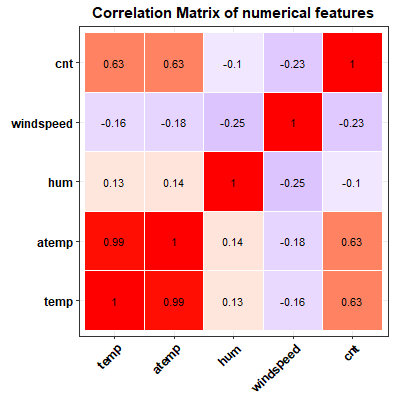
\includegraphics[width=0.8\linewidth]{images/VK_PDP_3_Num_Correlation_Matrix} 

}

\caption{Matrix of Pearson correlation coefficients between all numerical variables extracted from the bike-sharing dataset.}\label{fig:Figure03}
\end{figure}

Due to their strong correlation, `temp' (\(x_7\)) and `atemp' (\(x_8\))
perfectly qualify for our analysis of the impact of dependent features
on PDPs. In order to compare the partial dependence curve with and
without the influence of dependent features, we compute PDPs based on
the following models:

\begin{equation}
 y \sim x_1 + x_2 + x_4 + x_5 + x_6 + \mathbf{x_7}  + x_9 + x_{10} \label{eq:1} 
\end{equation}

\begin{equation}
 y \sim x_1 + x_2 + x_4 + x_5 + x_6 + \mathbf{x_8}  + x_9 + x_{10} \label{eq:2}
\end{equation}

\begin{equation}
 y \sim x_1 + x_2 + x_4 + x_5 + x_6 \mathbf{+ x_7 + x_8} + x_9 + x_{10} \label{eq:3}
\end{equation}

Please note that the representation of the different models with the
feature variables connected via `+' shall, in this context, not be read
as a (linear) regression model where all coefficients are equal to 1,
but rather as a combination of applicable feature variables to explain
\(y\). The (non-)linear effect of each variable is modelled
individually, depending on the observed values and the learner.

While model \eqref{eq:1} and \eqref{eq:2} only take one of the two
substituting variables into account, \eqref{eq:3} considers both `temp'
and `atemp' in one and the same model. Figures \ref{fig:Figure04},
\ref{fig:Figure05} and \ref{fig:Figure06} compare the associated PDPs
for the different learning algorithms. Note that `season' (\(x_1\)) and
`mnth' (\(x_3\)) are not taken into account in combination with \(x_7\)
and/or \(x_8\), since there are meaningful associations between those
variables, too, as we will show in chapter \ref{NumCat}. At this stage
we want to illustrate the isolated effect of the dependence between the
two numerical variables.

\begin{figure}

{\centering 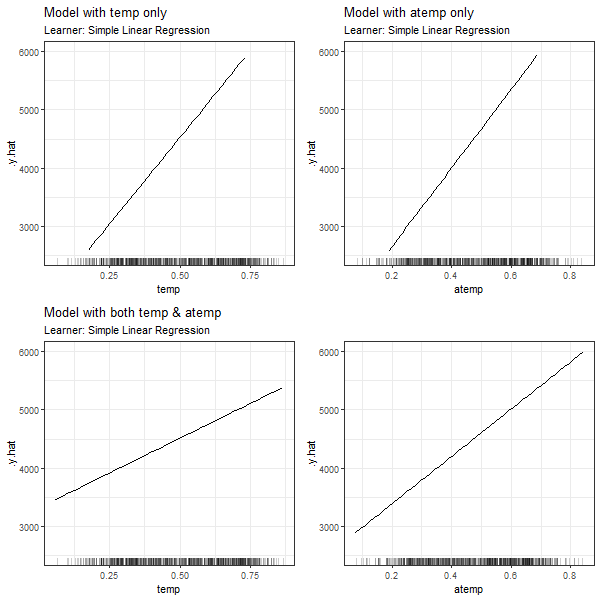
\includegraphics[width=0.8\linewidth]{images/VK_PDP_4_Correlated_numerical_LM} 

}

\caption{PDPs based on Linear Regression learner for 'temp' in model 3.1 (top left), 'atemp' in model 3.2 (top right), 'temp' in model in model 3.3 (bottom left) and 'atemp' in model 3.3 (bottom right).}\label{fig:Figure04}
\end{figure}

\begin{figure}

{\centering 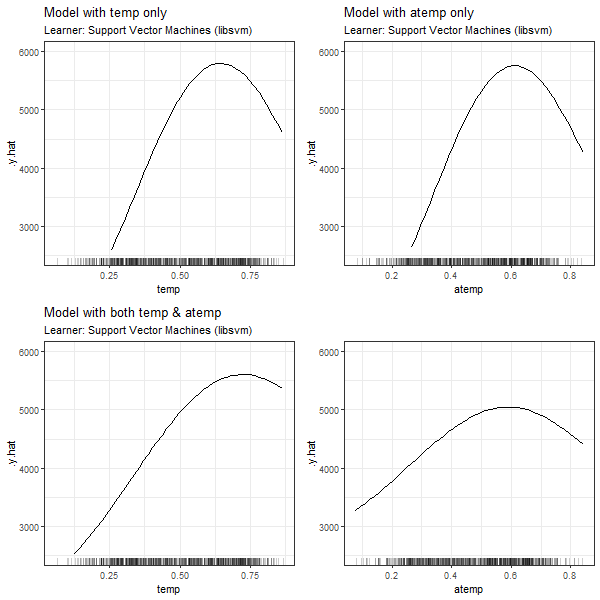
\includegraphics[width=0.8\linewidth]{images/VK_PDP_5_Correlated_numerical_SVM} 

}

\caption{PDPs based on Support Vector Machines learner for 'temp' in model 3.1 (top left), 'atemp' in model 3.2 (top right), 'temp' in model in model 3.3 (bottom left) and 'atemp' in model 3.3 (bottom right).}\label{fig:Figure05}
\end{figure}

\begin{figure}

{\centering 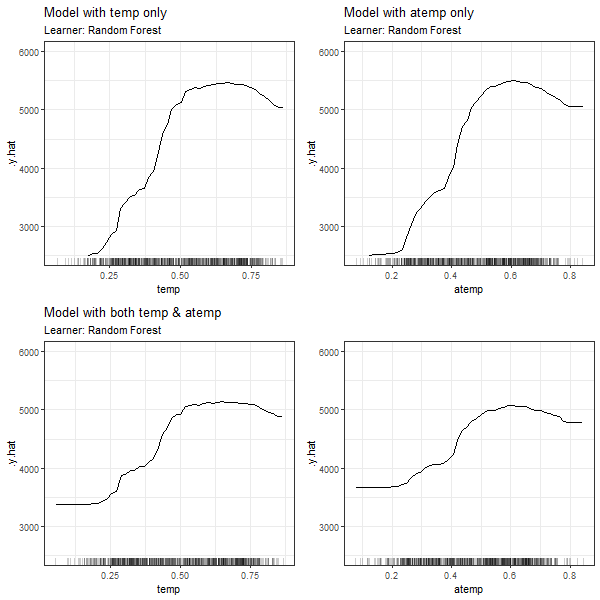
\includegraphics[width=0.8\linewidth]{images/VK_PDP_6_Correlated_numerical_RF} 

}

\caption{PDPs based on Random Forest learner for 'temp' in model 3.1 (top left), 'atemp' in model 3.2 (top right), 'temp' in model in model 3.3 (bottom left) and 'atemp' in model 3.3 (bottom right).}\label{fig:Figure06}
\end{figure}

In all cases, we can see that the features' effect on the prediction is
basically the same for \(x_7\) and \(x_8\), if only one of the dependent
variables is used for modelling (see PDPs in top left and top right
corners). If both `temp' and `atemp' are relevant for the prediction of
\(y\), each feature's impact is smoothened and neither the PDP for
\(x_7\) nor the one for \(x_8\) seems to properly reflect the true
effect of the temperature on the count of bike rentals.

\subsection{Dependency between Categorical
Features}\label{dependency-between-categorical-features}

In order to measure the association between two categorical features, we
calculate the corrected contingency coefficient, which is based on the
\(\chi^2\)-statistic. Other than the Pearson correlation coefficient,
the corrected contingency coefficient is a measure of association
\(\in [0,1]\) which can only indicate the strength but not the direction
of the variables' relationship \citep{fahrmeir2016statistik}. For the
categorical features in the Bike-Sharing dataset, we observe the values
stated in figure \ref{fig:Figure07}.

\begin{figure}

{\centering 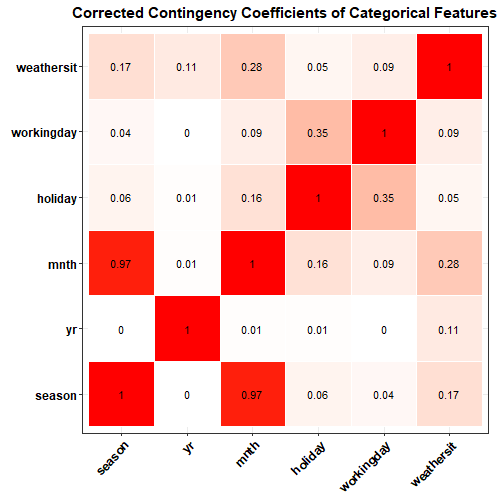
\includegraphics[width=0.8\linewidth]{images/VK_PDP_7_Cat_Correlation_Matrix} 

}

\caption{Matrix of corrected contingency coefficients between all categorical variables extracted from the bike-sharing dataset.}\label{fig:Figure07}
\end{figure}

The only combination of categorical features with an exceptionally high
corrected contingency coefficient, is `season' (\(x_1\)) and `mnth'
(\(x_3\)). Also from a content-related point of view, this finding is no
surprise, since both variables measure the time of the year. For the
computation of the respective PDPs, we use the following models:

\begin{equation} 
y \sim \mathbf{x_1} + x_2 + x_4 + x_5 + x_6 + x_9 + x_{10} \label{eq:4}
\end{equation}

\begin{equation}
y \sim x_2 +\mathbf{x_3} + x_4 + x_5 + x_6 + x_9 + x_{10} \label{eq:5}
\end{equation}

\begin{equation}
y \sim \mathbf{x_1} + x_2 + \mathbf{x_3} + x_4 + x_5 + x_6 + x_9 + x_{10} \label{eq:6}
\end{equation}

The approach is equivalent to the numeric case, with model \eqref{eq:4}
containing only `season' and \eqref{eq:5} only `mnth', while both
dependent features are part of model \eqref{eq:6}. The impact on the PDPs
for categorical features are shown in figures \ref{fig:Figure08},
\ref{fig:Figure09} and \ref{fig:Figure10}.

\begin{figure}

{\centering 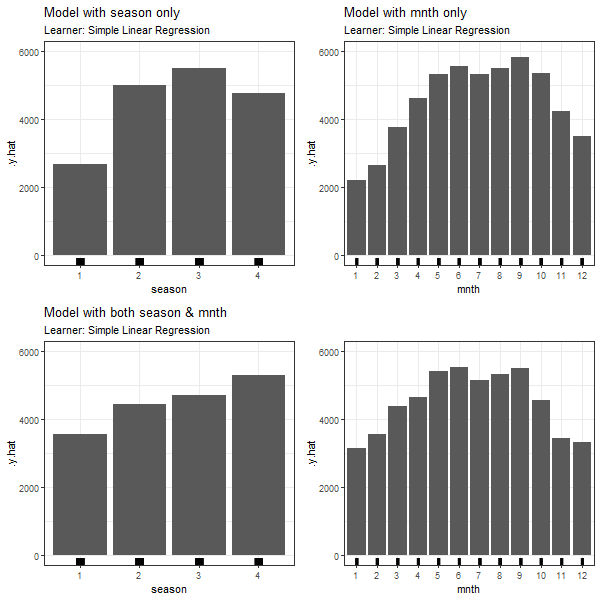
\includegraphics[width=0.8\linewidth]{images/VK_PDP_8_Correlated_categorical_LM} 

}

\caption{PDPs based on Linear Regression learner for 'season' in model 3.4 (top left), 'mnth' in model 3.5 (top right), 'season' in model in model 3.6 (bottom left) and 'mnth' in model 3.6 (bottom right).}\label{fig:Figure08}
\end{figure}

\begin{figure}

{\centering 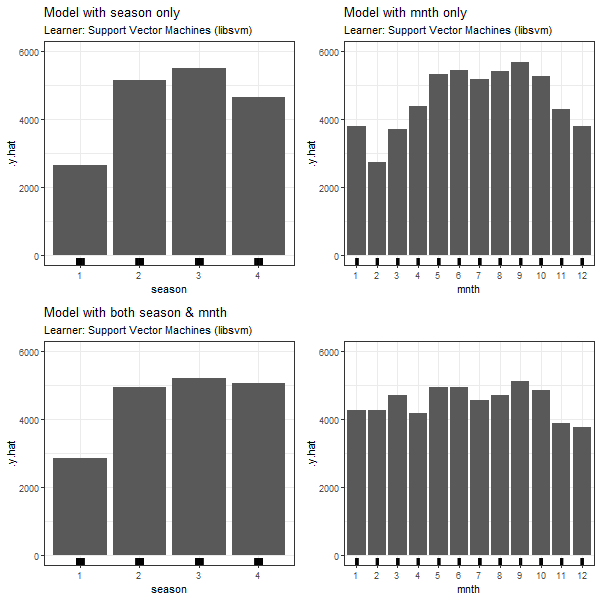
\includegraphics[width=0.8\linewidth]{images/VK_PDP_9_Correlated_categorical_SVM} 

}

\caption{PDPs based on Support Vector Machines learner for 'season' in model 3.4 (top left), 'mnth' in model 3.5 (top right), 'season' in model in model 3.6 (bottom left) and 'mnth' in model 3.6 (bottom right).}\label{fig:Figure09}
\end{figure}

\begin{figure}

{\centering 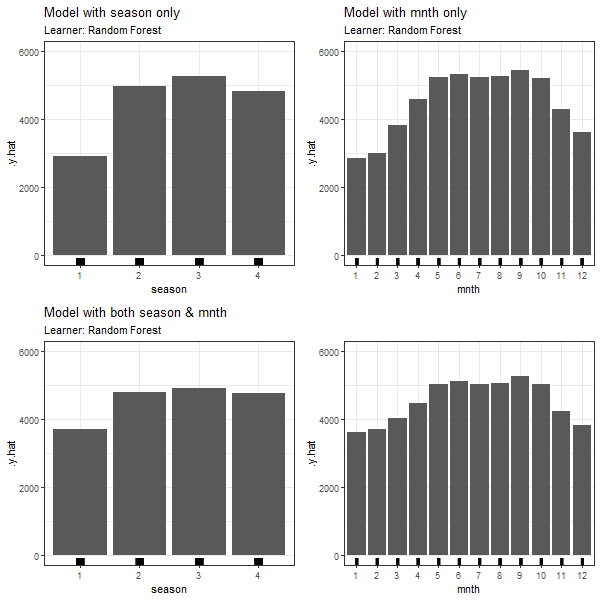
\includegraphics[width=0.8\linewidth]{images/VK_PDP_10_Correlated_categorical_RF} 

}

\caption{PDPs based on Random Forest learner for 'season' in model 3.4 (top left), 'mnth' in model 3.5 (top right), 'season' in model in model 3.6 (bottom left) and 'mnth' in model 3.6 (bottom right).}\label{fig:Figure10}
\end{figure}

Again, in all PDPs based on the different learning algorithms, the
results between models with and without dependent features are
diverging. The predicted number of bike rentals between the
seasons/months shows a stronger variation when modelled without feature
dependencies.

\subsection{Dependency between Numerical and Categorical
Features}\label{NumCat}

Our third dependency scenario seeks to provide an example for a strong
correlation between a numerical and a categorical feature. For this
constellation, neither the Pearson correlation nor the contingency
coefficient are applicable as such, since both methods are limited to
their respective classes of variables.

We can, however, fit a linear model to explain the numeric variable
through the categorical feature. By doing so, we produce another
numerical variable, the fitted values. In a next step, we can calculate
the Pearson correlation coefficient between the observed and the fitted
values of the numerical feature. The resulting measure of association
lies within the interval \([0,1]\) and is equivalent to the square root
of the linear model's variance explained (\(R^2\))
\citep{fahrmeir2013regression}. For this reason, we refer to the measure
as `variance-explained measure'.

When applying this procedure to the categorical feature `season'
(\(x_1\)) and the numerical feature `temp' (\(x_7\)), we find that with
a variance-explained value of 0.83, there seems to be a reasonable
association between the two features. The PDPs are derived through the
following models:

\begin{equation}
y \sim \mathbf{x_1} + x_2 + x_4 + x_5 + x_6 + x_9 + x_{10} \label{eq:7}
\end{equation}

\begin{equation}
y \sim x_1 + x_2 + x_4 + x_5 + x_6 + \mathbf{x_7}+ x_9 + x_{10} \label{eq:8}
\end{equation}

\begin{equation}
y \sim \mathbf{x_1} + x_2  + x_4 + x_5 + x_6 +\mathbf{x_7}+ x_9 + x_{10} \label{eq:9}
\end{equation}

Figure \ref{fig:Figure11}, \ref{fig:Figure12} and \ref{fig:Figure13}
present the partial dependence plots for the three underlying machine
learning algorithms (LM, SVM and RF) defined for the purpose of our
analysis.

\begin{figure}

{\centering 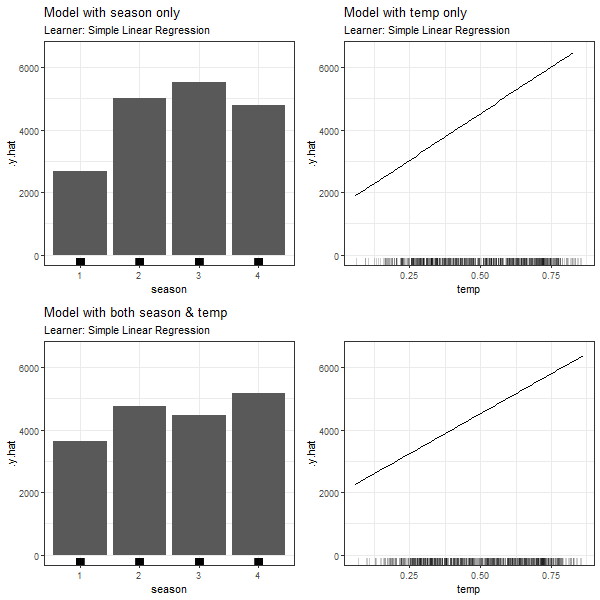
\includegraphics[width=0.8\linewidth]{images/VK_PDP_11_Correlated_cat_num_LM} 

}

\caption{PDPs based on Linear Regression learner for 'season' in model 3.4 (top left), 'temp' in model 3.5 (top right), 'season' in model in model 3.6 (bottom left) and 'temp' in model 3.6 (bottom right).}\label{fig:Figure11}
\end{figure}

\begin{figure}

{\centering 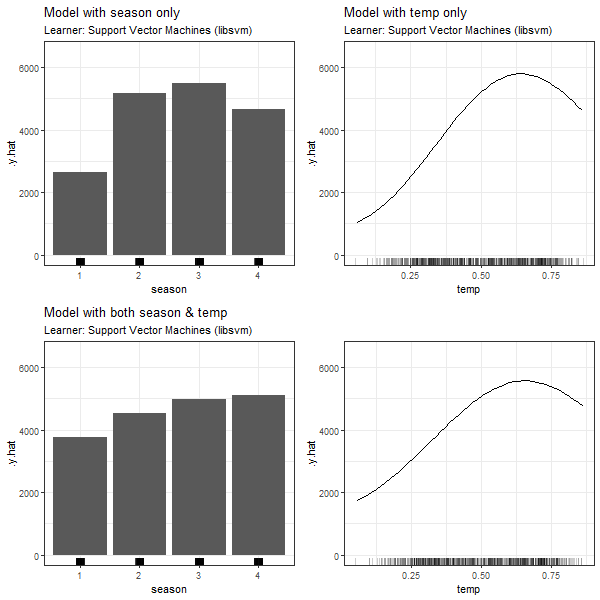
\includegraphics[width=0.8\linewidth]{images/VK_PDP_12_Correlated_cat_num_SVM} 

}

\caption{PDPs based on Support Vector Machines learner for 'season' in model 3.4 (top left), 'temp' in model 3.5 (top right), 'season' in model in model 3.6 (bottom left) and 'temp' in model 3.6 (bottom right).}\label{fig:Figure12}
\end{figure}

\begin{figure}

{\centering 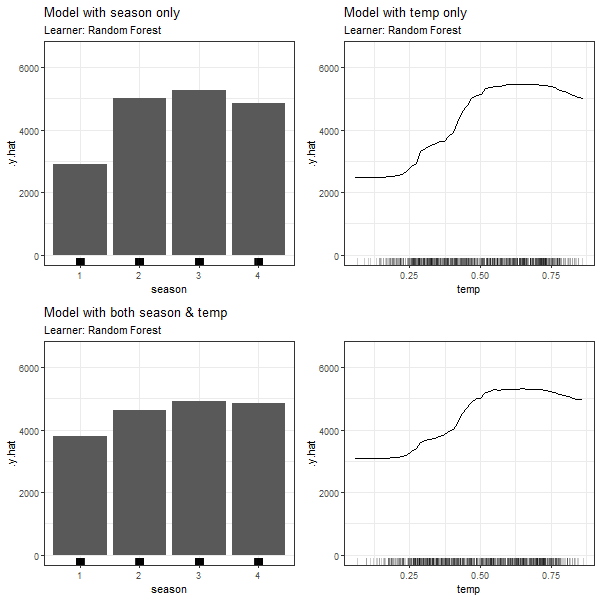
\includegraphics[width=0.8\linewidth]{images/VK_PDP_13_Correlated_cat_num_RF} 

}

\caption{PDPs based on Random Forest learner for 'season' in model 3.4 (top left), 'temp' in model 3.5 (top right), 'season' in model in model 3.6 (bottom left) and 'temp' in model 3.6 (bottom right).}\label{fig:Figure13}
\end{figure}

Compared to the first two scenarios, we observe a more moderate
difference between the PDPs when comparing model \eqref{eq:7} and
\eqref{eq:8} containing just one of the dependent features to the full
model \eqref{eq:9}. The weaker association between the two variables, in
contrast to scenario 1 and 2, could be an explanation for this
observation. It is, however, evident that the dependency structure
between two feature variables, irrespective of their class, does impact
the partial dependence plot.

\section{Dependent Features: Simulated Data}\label{SimulatedData}

A major disadvantage of the analysis of PDPs on the basis of real data
examples is, that we cannot exclude other factors to play a role. As an
example, underlying interactions could have an impact on the PDP and
hide the true effect of a feature on the predicted target variable
\citep{molnar2019}. In order to illustrate the isolated impact of
dependent variables in the feature space, we have simulated data in
different settings, which we will discuss in this chapter.

\subsection{Simulation Settings: Numerical
Features}\label{simulation-settings-numerical-features}

For a start, the different settings of simulations used for our
investigation shall be introduced. Just like in chapter 2, we are
separately looking at different classes of variables and different
machine learning algorithms (LM, RF and SVM). PDPs for independent,
correlated and dependent numerical features are computed for each of the
following data generating processes (DGP), which describe the true
impact of the features on \(y\):

\begin{itemize}
\tightlist
\item
  Setting 1: Linear Dependence:\\

  \begin{equation}
  y = x_1 + x_2 + x_3 + \varepsilon \label{eq:10}
  \end{equation}
\item
  Setting 2: Nonlinear Dependence in \(x_1\):\\

  \begin{equation}
  y = \sin{( \, 3*x_1 ) \,} + x_2 + x_3 + \varepsilon \label{eq:11}
  \end{equation}
\item
  Setting 3: Missing informative feature \(x_3\)\\

  \begin{equation}
  y = x_1 + x_2 + x_3 + \varepsilon \label{eq:12}
  \end{equation}

  with \(x_3\) relevant for the DGP but unconsidered in the machine
  learning model.
\end{itemize}

In the independent case, the feature variables \(x_1\), \(x_2\) and
\(x_3\) have been drawn from a gaussian distribution with \(\mu = 0\),
\(\sigma^2 = 1\) and a correlation coefficient of \(\rho_{ij} = 0\)
\(\forall\) \(i \ne j\), \(i,j \in \{1,2,3\}\).\\
The correlated case is based on the same parameters for \(\mu\) and
\(\sigma^2\), but a correlation coefficient of
\(\rho_{12} = \rho_{21} = 0.90\), i.e.~a relatively strong linear
association between \(x_1\) and \(x_2\), and \(\rho_{ij} = 0\)
otherwise.\\
The dependent case describes the event of perfect multicollinearity,
where \(x_2\) is a duplicate of \(x_1\), based on the data generated in
the independent case.\\
The target variable \(y\) results from the respective DGP with an error
term \(\varepsilon \sim N(0, \sigma^2_\varepsilon)\) and
\(\sigma^2_\varepsilon\) depending on the feature values.

One source of variation in the PDPs is the simulation of the data
itself. For this reason, the process has been repeated 20 times for each
analysis and the resulting PDP curves are shown as gray lines in the
plots below. The thicker, black line represents the average partial
dependence curve over these 20 simulations and the error bars indicate
their variation. Additionally, a red line represents the true effect of
the feature for which the PDP is computed. In all cases, the simulations
are based on a number of 500 observations and grid size 50.

Since in the dependent case, \(x_2\) is simply a duplicate of \(x_1\),
the DGP could also be written as \(y = 2*x_1 + x_3 + \varepsilon\) in
setting \eqref{eq:10} and \eqref{eq:12} and
\(y = \sin{( \, 3*x_1 ) \,} + x_1 + x_3 + \varepsilon\) in setting
\eqref{eq:11}. For the purpose of this analysis, we are looking at each of
the three features' PDP separately. However, in order to illustrate the
aforementioned, the common effect of \(x_1\) and \(x_2\) on the
prediction is added to the plots as dashed blue line.

\subsection{Simulation of Setting 1: Linear
Dependence}\label{simulation-of-setting-1-linear-dependence}

\subsubsection{PDPs based on Linear
Model}\label{pdps-based-on-linear-model}

The results of our simulations in setting 1 based on the Linear Model
are shown in figure \ref{fig:Figure14}:

\begin{figure}

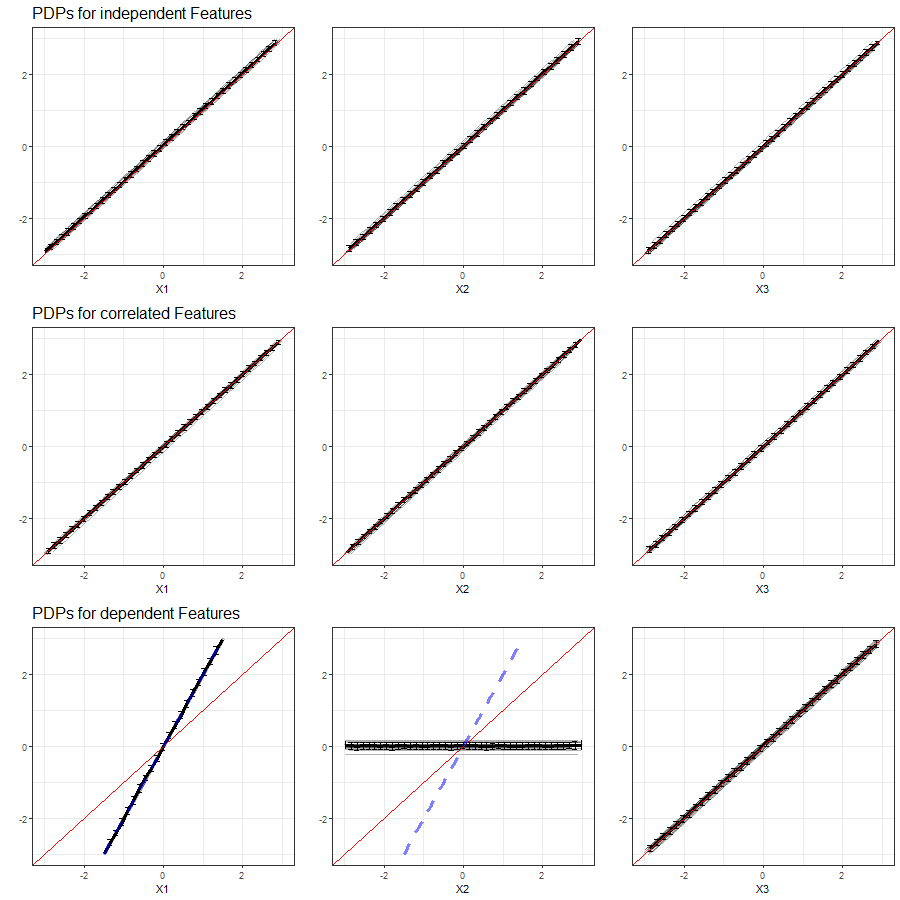
\includegraphics[width=1\linewidth]{images/VK_PDP_14_Set1_LM} \hfill{}

\caption{PDPs for features $x_1$, $x_2$ and $x_3$ (left to right) in Setting 1, based on multiple simulations with Linear Model as learning algorithm. Top row shows independent case, second row the correlated case and bottom row the dependent case. The red line represents the true effect of the respective feature on $y$, the blue dashed line is the true commmon effect of $x_1$ and $x_2$.}\label{fig:Figure14}
\end{figure}

Across all simulations, there is hardly any variation between the PDPs
based on the Linear Model. In the independent case, the PDPs for each
feature adequately reflect the linear dependency structure. The effect
is equivalent in each PDP, since all features have the same impact and
are independent from each other. From the PDPs in the second row of
figure \ref{fig:Figure14} we see that even with a relatively strong
correlation of features \(x_1\) and \(x_2\), the PDPs adequately reflect
the linear dependency structure when predictions are computed from the
Linear Model. In the event of perfect multicollinearity, the PDP for one
of the dependent features (\(x_2\)) fails, while the corresponding PDP
for the other feature (\(x_1\)) reflects the common effect of both. The
PDP for feature \(x_3\) adequately reveals its linear effect on \(y\).

\subsubsection{PDPs based on Random
Forest}\label{pdps-based-on-random-forest}

The results of our simulations in setting 1 based on Random Forest are
shown in figure \ref{fig:Figure15}:

\begin{figure}

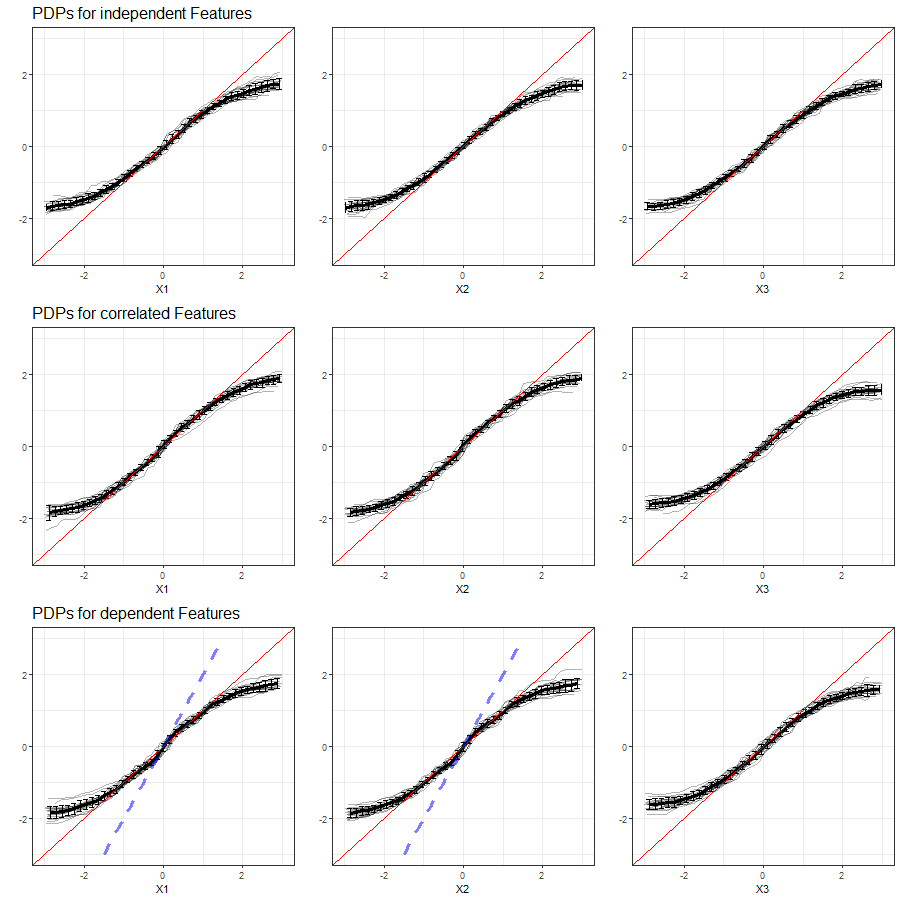
\includegraphics[width=1\linewidth]{images/VK_PDP_15_Set1_RF} \hfill{}

\caption{PDPs for features $x_1$, $x_2$ and $x_3$ (left to right) in Setting 1, based on multiple simulations with Random Forest as learning algorithm. Top row shows independent case, second row the correlated case and bottom row the dependent case. The red line represents the true effect of the respective feature on $y$, the blue dashed line is the true commmon effect of $x_1$ and $x_2$.}\label{fig:Figure15}
\end{figure}

Compared to the LM, there is a little more variance between the
individual PDP curves produced from RF as learner. Furthermore, the
partial dependence plots cannot adequately reflect the linear dependency
structure, particularly at the margins of the feature's distribution.
Again, there is no visual differentiation between the different features
in the first row of figure \ref{fig:Figure15} due to their independence.
Besides, the computation of PDPs based on Random Forest does not produce
significantly worse results when two features are correlated and the
relationship between all variables and \(y\) is linear.\\
When comparing the PDPs subject to perfect multicollinearity to those in
the correlated case, a slightly increased variation in the individual
PDP curves is observed. Other than in the Linear Model, the learner is
not able to reveal the true common effect of \(x_1\) and \(x_2\).

\subsubsection{PDPs based on Support Vector
Machines}\label{pdps-based-on-support-vector-machines}

The results of our simulations in setting 1 based on Support Vector
Machines are shown in figure \ref{fig:Figure16}:

\begin{figure}

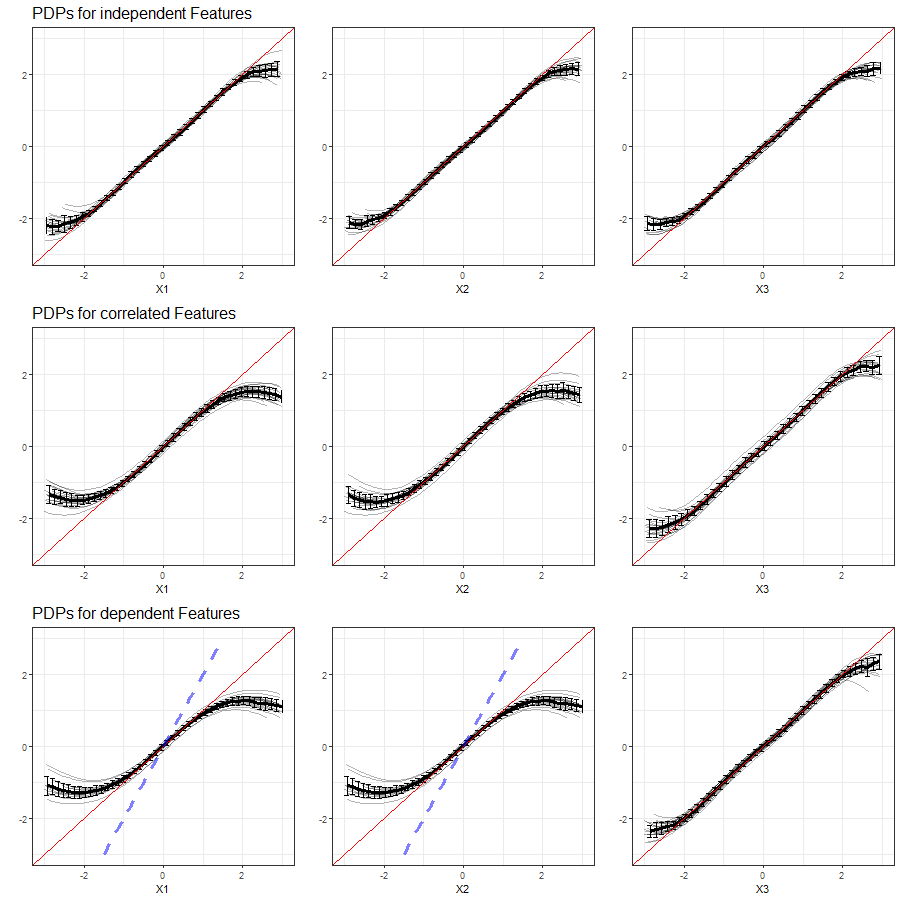
\includegraphics[width=1\linewidth]{images/VK_PDP_16_Set1_SVM} \hfill{}

\caption{PDPs for features $x_1$, $x_2$ and $x_3$ (left to right) in Setting 1, based on multiple simulations with Support Vector Machines as learning algorithm. Top row shows independent case, second row the correlated case and bottom row the dependent case. The red line represents the true effect of the respective feature on $y$, the blue dashed line is the true commmon effect of $x_1$ and $x_2$.}\label{fig:Figure16}
\end{figure}

Support Vector Machines as learning algorithms are able to reproduce the
respective feature's linear effect on the prediction fairly adequate in
case of independence. The accuracy decreases in the margins of the
feature's distribution. With two correlated features, the interval of
predicted values of both correlated features becomes smaller, while the
learner produces the same `shape' of its effect, both for \(x_1\) and
\(x_2\). The same observation is made in the event of two identical
features (dependent case), but even more evident with PDP curves
increasingly deviating from the true effect. Other than in the LM, none
of the PDPs for the dependent features reveals the true common effect of
\(x_1\) and \(x_2\).

\subsection{Simulation of Setting 2: Nonlinear
Dependence}\label{simulation-of-setting-2-nonlinear-dependence}

In simulation setting 2 we are looking at a DGP with a nonlinear
relationship of \(x_1\) and \(y\) and a linear impact of \(x_2\) and
\(x_3\). Due to the nonlinearity in one of the features, it is clear
that the LM would not deliver accurate results. For this reason, in this
chapter we will restrict our analysis to RF and SVM.

\subsubsection{PDPs based on Random
Forest}\label{pdps-based-on-random-forest-1}

The results of our simulations in setting 2 based on Random Forest are
shown in figure \ref{fig:Figure17}:

\begin{figure}

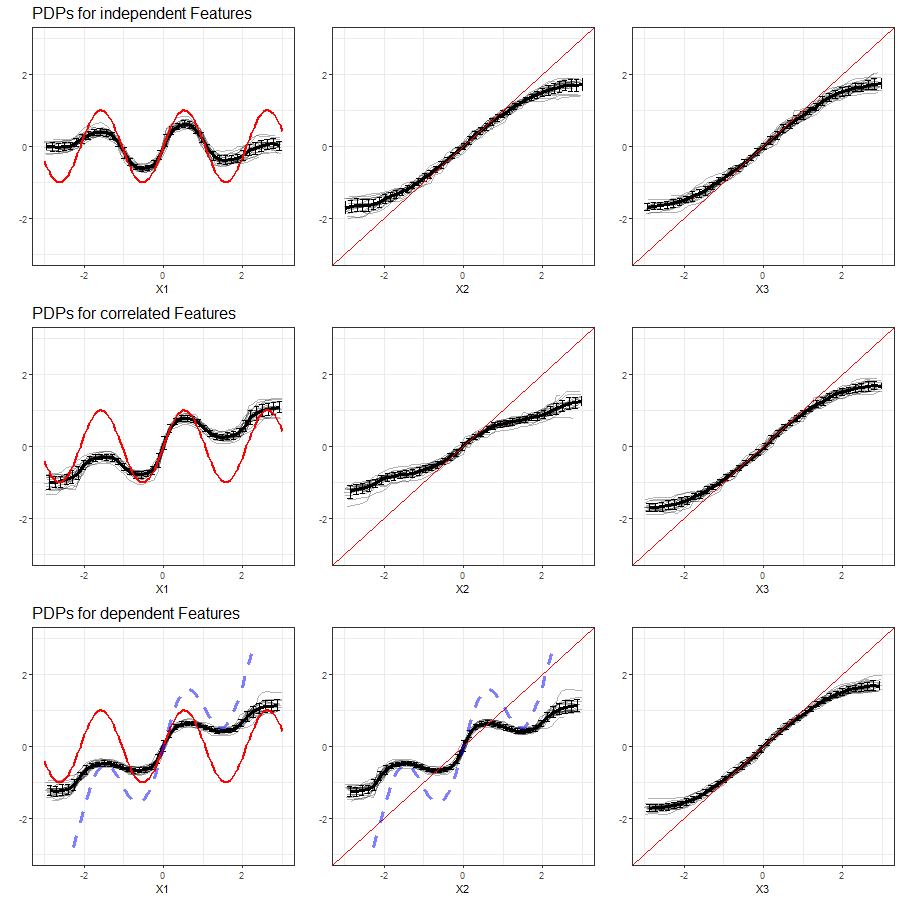
\includegraphics[width=1\linewidth]{images/VK_PDP_17_Set2_RF} \hfill{}

\caption{PDPs for features $x_1$, $x_2$ and $x_3$ (left to right) in Setting 2, based on multiple simulations with Random Forest as learning algorithm. Top row shows independent case, second row the correlated case and bottom row the dependent case. The red line represents the true effect of the respective feature on $y$, the blue dashed line is the true commmon effect of $x_1$ and $x_2$.}\label{fig:Figure17}
\end{figure}

From the PDP of feature \(x_1\) in the first row of figure
\ref{fig:Figure17} it is evident that Random Forest as a learner can
retrace the nonlinear effect of the variable quite well, except for the
margin areas of the feature distribution. The PDPs for feature \(x_2\)
and \(x_3\) are equivalent to those in simulation setting \eqref{eq:10}.\\
With a simulated correlation between features \(x_1\) and \(x_2\) and a
nonlinear relationship of \(x_1\) and \(y\), the ability of the
respective PDPs to illustrate the feature's effect degrades with RF as
learner. Both the nonlinear effect of \(x_1\) and the linear effect of
\(x_2\) are distorted in the PDPs.\\
In the event of perfect multicollinearity, the PDPs for the involved
feature variables fail even more. In contrast to the correlated case, we
can observe that both curves take on a similar shape, which very roughly
approximates the common effect.

\subsubsection{PDPs based on Support Vector
Machines}\label{pdps-based-on-support-vector-machines-1}

The results of our simulations in setting 2 based on SVM are shown in
figure \ref{fig:Figure18}:

\begin{figure}

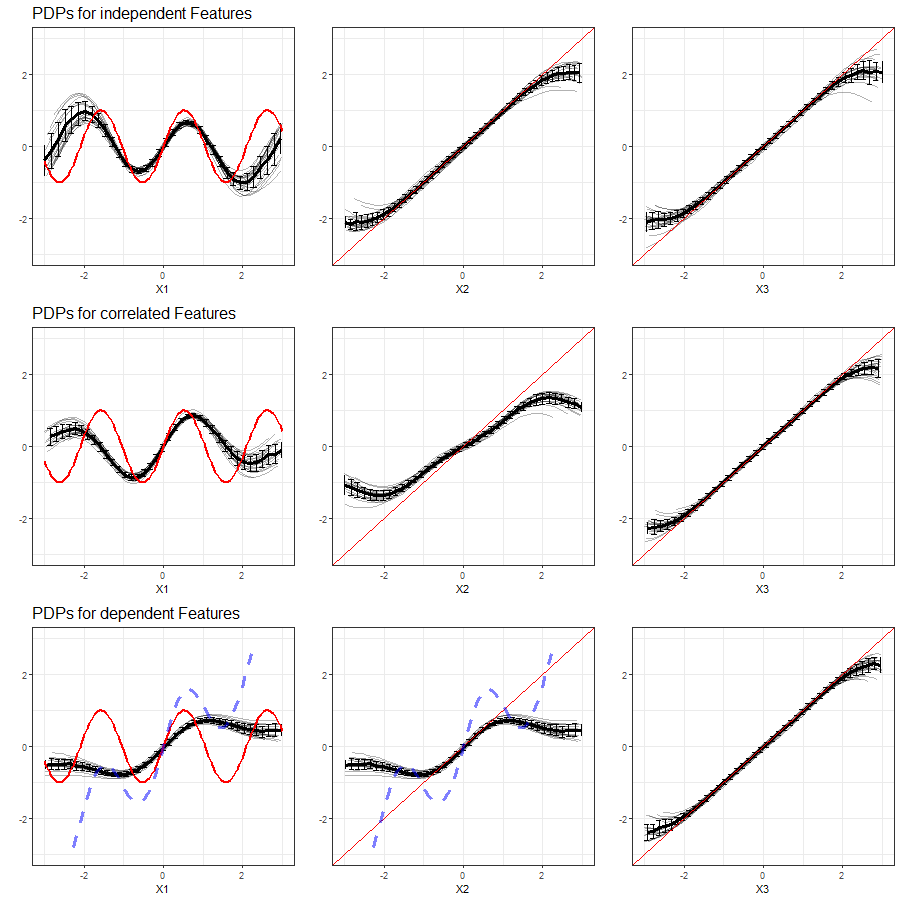
\includegraphics[width=1\linewidth]{images/VK_PDP_18_Set2_SVM} \hfill{}

\caption{PDPs for features $x_1$, $x_2$ and $x_3$ (left to right) in Setting 2, based on multiple simulations with SVM as learning algorithm. Top row shows independent case, second row the correlated case and bottom row the dependent case. The red line represents the true effect of the respective feature on $y$, the blue dashed line is the true commmon effect of $x_1$ and $x_2$.}\label{fig:Figure18}
\end{figure}

The findings derived from PDPs based on Random Forest are equivalently
applicable to Support Vector Machines as machine learning algorithm. In
the event of independent features, the PDPs can fairly well reveal the
true feature effects, despite in the margins of the feature
distrubutions. With strongly correlated or even dependent features, this
ability vanishes and the PDPs of the affected features transform towards
the variables' common effect.

\subsection{\texorpdfstring{Simulation of Setting 3: Missing informative
feature
\(x_3\)}{Simulation of Setting 3: Missing informative feature x\_3}}\label{simulation-of-setting-3-missing-informative-feature-x_3}

In simulation setting 3, we assume that there are three variables with
an impact on the data generating process of \(y\). In the training
process of the machine learning model, only two of those are considered.
Consequently, when looking at the PDPs, we only compare the independent,
the correlated and the dependent case for \(x_1\) and \(x_2\)
respectively.

\subsubsection{PDPs based on Linear
Model}\label{pdps-based-on-linear-model-1}

The results of our simulations in setting 3 based on the Linear Model
are shown in figure \ref{fig:Figure19}:

\begin{figure}

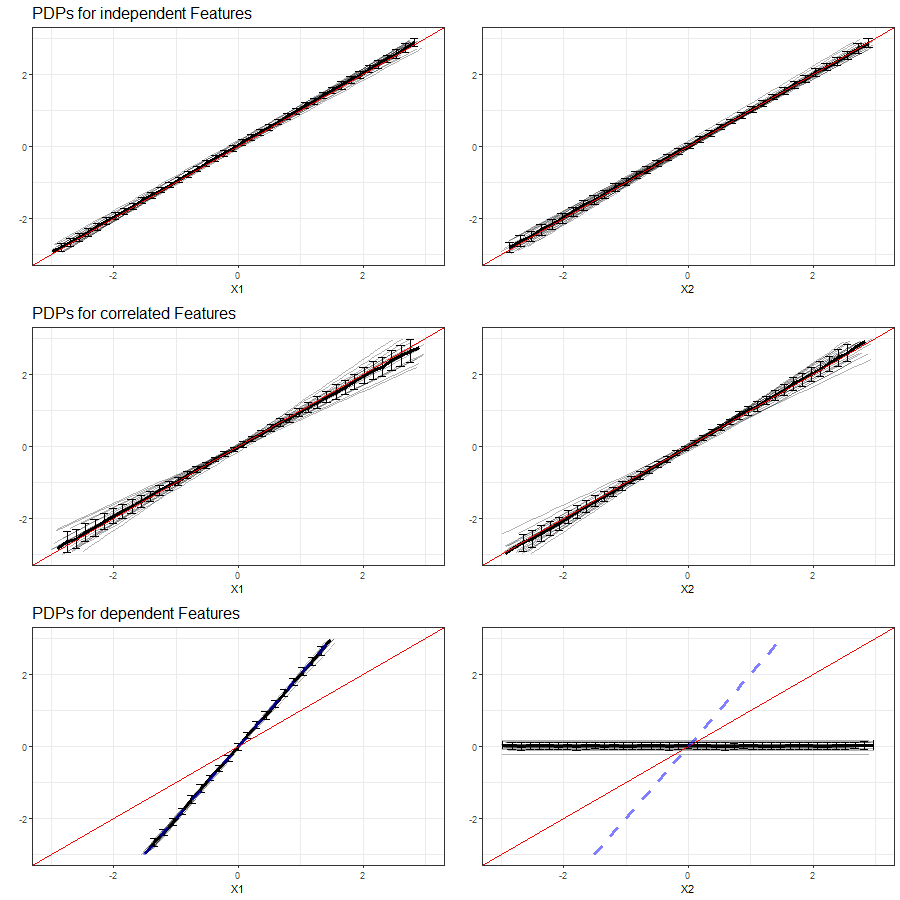
\includegraphics[width=1\linewidth]{images/VK_PDP_19_Set3_LM} \hfill{}

\caption{PDPs for features $x_1$ (left) and $x_2$  (right) in Setting 3, based on multiple simulations with LM as learning algorithm. Top row shows independent case, second row the correlated case and bottom row the dependent case. The red line represents the true effect of the respective feature on $y$, the blue dashed line is the true commmon effect of $x_1$ and $x_2$.}\label{fig:Figure19}
\end{figure}

Compared to the PDPs of independent features the Linear Model produced
in setting \eqref{eq:10}, the variation in individual PDPs is slightly
higher with missing information from \(x_3\). Overall, the learner can
adequately reflect the linear feature effects of \(x_1\) and \(x_2\).\\
The increase in variablility between the individual PDPs is even more
evident in the correlated case. On average, we still obtain the true
linear effect of the correlated features, but there are some individual
curves which do indicate a steeper or more moderate slope.\\
The PDPs drawn on basis of the Linear Model and dependent features
indicate that for both individual features, the PDP consistently
provides false effects on the predicted outcome. While both effects are
actually linear with a slope of 1, the PDP for \(x_1\) shows a steeper
increase and \(x_2\) fails completely. Nonetheless, the PDP for \(x_1\)
does reflect the common effect of both variables together.

\subsubsection{PDPs based on Random
Forest}\label{pdps-based-on-random-forest-2}

The results of our simulations in setting 3 based on Random Forest are
shown in figure \ref{fig:Figure20}:

\begin{figure}

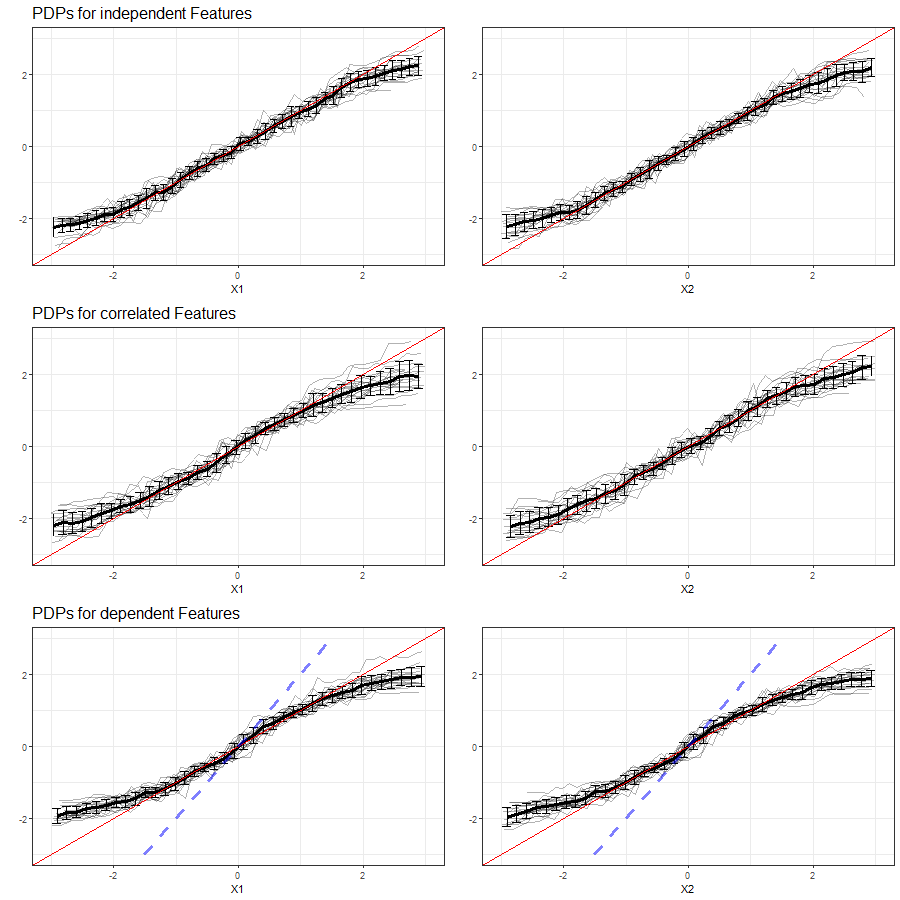
\includegraphics[width=1\linewidth]{images/VK_PDP_20_Set3_RF} \hfill{}

\caption{PDPs for features $x_1$ (left) and $x_2$  (right) in Setting 3, based on multiple simulations with RF as learning algorithm. Top row shows independent case, second row the correlated case and bottom row the dependent case. The red line represents the true effect of the respective feature on $y$, the blue dashed line is the true commmon effect of $x_1$ and $x_2$.}\label{fig:Figure20}
\end{figure}

Compared to setting \eqref{eq:10}, where all relevant feature variables
were taken into account for the training of the model, the variation in
PDP curves in setting \eqref{eq:12} is larger. Between features \(x_1\)
and \(x_2\), which are independent, there is no systematic difference
traceable from the PDPs.\\
Other than an increased variability between the individual PDP curves
and a slightly tighter prediction interval, with correlated features and
Random Forest as learner, there is no apparent deviation to the PDPs of
independent features.\\
In accordance with the observations made in setting \eqref{eq:10}, the
interval of predicted values for dependent features become even smaller
while the PDP curves further deviate from the true effect. Neither the
individual effect of each feature, nor their common effect are
illustrated adequately.

\subsubsection{PDPs based on Support Vector
Machines}\label{pdps-based-on-support-vector-machines-2}

The results of our simulations in setting 3 based on Support Vector
Machines are shown in figure \ref{fig:Figure21}:

\begin{figure}

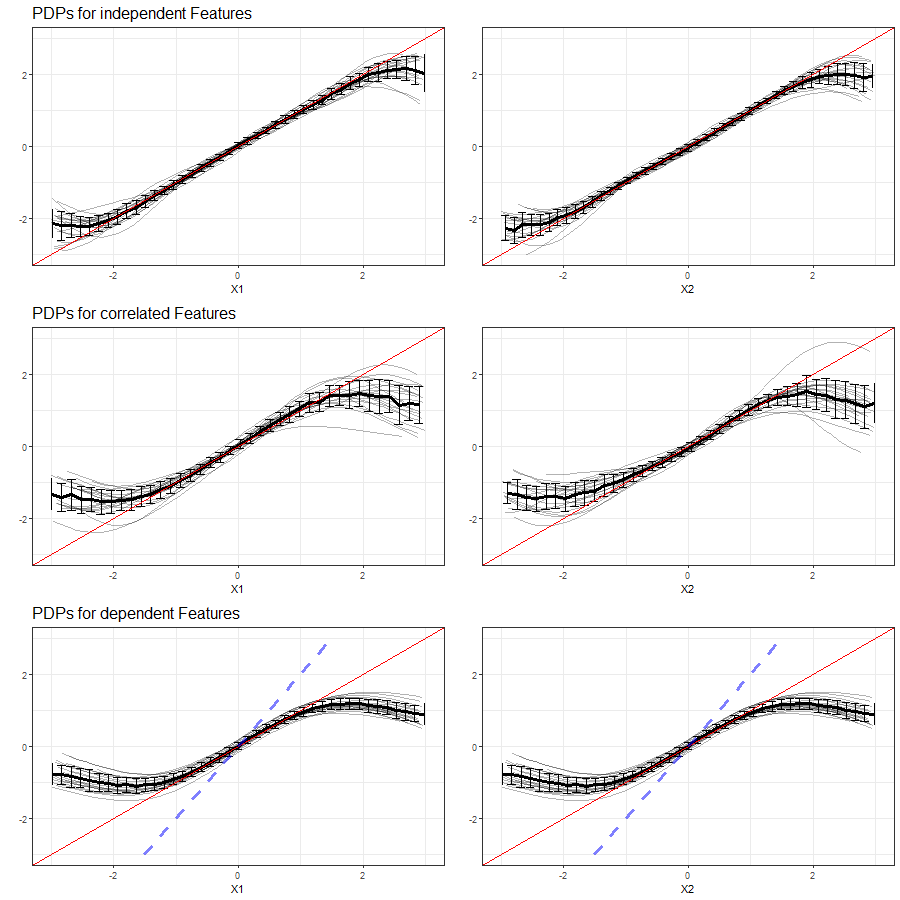
\includegraphics[width=1\linewidth]{images/VK_PDP_21_Set3_SVM} \hfill{}

\caption{PDPs for features $x_1$ (left) and $x_2$  (right) in Setting 3, based on multiple simulations with SVM as learning algorithm. Top row shows independent case, second row the correlated case and bottom row the dependent case. The red line represents the true effect of the respective feature on $y$, the blue dashed line is the true commmon effect of $x_1$ and $x_2$.}\label{fig:Figure21}
\end{figure}

Similar to learning based on Random Forest, the SVM learner with missing
feature variable \(x_3\) produces a higher variability between the
simulated PDP curves. The margin areas, where the PDPs cannot adequately
reflect the linear dependence, are broader than in setting
\eqref{eq:10}.\\
In the event of the two remaining features \(x_1\) and \(x_2\) being
strongly correlated, the issue of larger variability between the
individual simulations aggravates and the ability to reveal the linear
effect ceases.\\
With a perfect multicollinearity of \(x_1\) and \(x_2\), the variablity
of the individual PDP curves becomes smaller, but at the same time the
models' ability to uncover the true linear effect vanishes. The interval
of predicted values is remarkably smaller than in the independent case.

\subsection{Simulation Settings: Categorical
Features}\label{simulation-settings-categorical-features}

In this chapter we want to investigate the impact of dependencies
between two categorical and between a categorical and a numerical
feature. For this purpose, we simulate data with a number of 1000
randomly drawn observations and three feature variables, where:

\begin{itemize}
\tightlist
\item
  \(x_1\) categorical variable \(\in \{0,1\}\),
\item
  \(x_2\) categorical variable \(\in \{A,B,C\}\),
\item
  \(x_3\) numerical variable with \(x_3 \sim N(\mu, \sigma^2)\).
\end{itemize}

All features are characterized by their linear relationship with the
target variable: \(y=x_1+x_2+x_3+\varepsilon\).

Again, in order to isolate the individual effects of two dependent
features on their respective PDPs, we define three different simulation
settings:

\textbf{1. Independent Case:} In this setting, the feature variables are
drawn independently from each other, i.e.~the observations are randomly
sampled with the following parameters:

\begin{itemize}
\tightlist
\item
  \(x_1: P(x_1=1)=P(x_1=0)=0.5\)
\item
  \(x_2: P(x_2=A)=0.475, P(x_2=B)=0.175, P(x_2=C)=0.35\)
\item
  \(x_3: P(x_3 \sim N(1,1))=0.5, P(x_3 \sim N(20,2))=0.5\)
\end{itemize}

The association between \(x_1\) and \(x_2\) can be measured by the
corrected contingency coefficient, which is rather low with a value of
0.10. In accordance with the approach in chapter \ref{NumCat}, we
calculate the association between \(x_1\) and \(x_3\) by means of the
variance-explained measure. With a value of 0.01 we take the
independence assumption as confirmed.

\textbf{2. Dependency between two categorical features:} In this
setting, \(x_1\) and \(x_2\) are depending on each each other, i.e.~the
observations are randomly sampled with the following parameters:

\begin{itemize}
\tightlist
\item
  \(x_1: P(x_1=1)=P(x_1=0)=0.5\)
\item
  \(x_2: \begin{cases} P(x_2=A)=0.90, P(x_2=B)=0.10, P(x_2=C)=0), \text{if } x_1=0, \\ P(x_2=A)=0.05, P(x_2=B)=0.25, P(x_2=C)=0.70), \text{if } x_1=1 \end{cases}\)
\item
  \(x_3: P(x_3 \sim N(1,1))=0.5, P(x_3 \sim N(20,2))=0.5\)
\end{itemize}

The corrected contingency coefficient of 0.94 comfirms a strong
association between features \(x_1\) and \(x_2\).

\textbf{3. Dependency between categorical and numerical features:} In
this setting, \(x_1\) and \(x_3\) are depending on each each other,
i.e.~the observations are randomly sampled with the following
parameters:

\begin{itemize}
\tightlist
\item
  \(x_1: P(x_1=1)=P(x_1=0)=0.5\)
\item
  \(x_2: P(x_2=A)=0.475, P(x_2=B)=0.175, P(x_2=C)=0.35\)
\item
  \(x_3: \begin{cases} x_3 \sim N(1,1), \text{if } x_1=0 \\ x_3 \sim N(20,2), \text{if } x_1=1 \end{cases}\)
\end{itemize}

With a value of 0.986, the variance-explained measure indicates a
substantial degree of dependency between \(x_1\) and \(x_3\).

\subsubsection{PDPs based on Linear
Model}\label{pdps-based-on-linear-model-2}

Figure \ref{fig:Figure22} shows the PDPs for all feature variables and
all simulation settings based on the Linear Model.

\begin{figure}

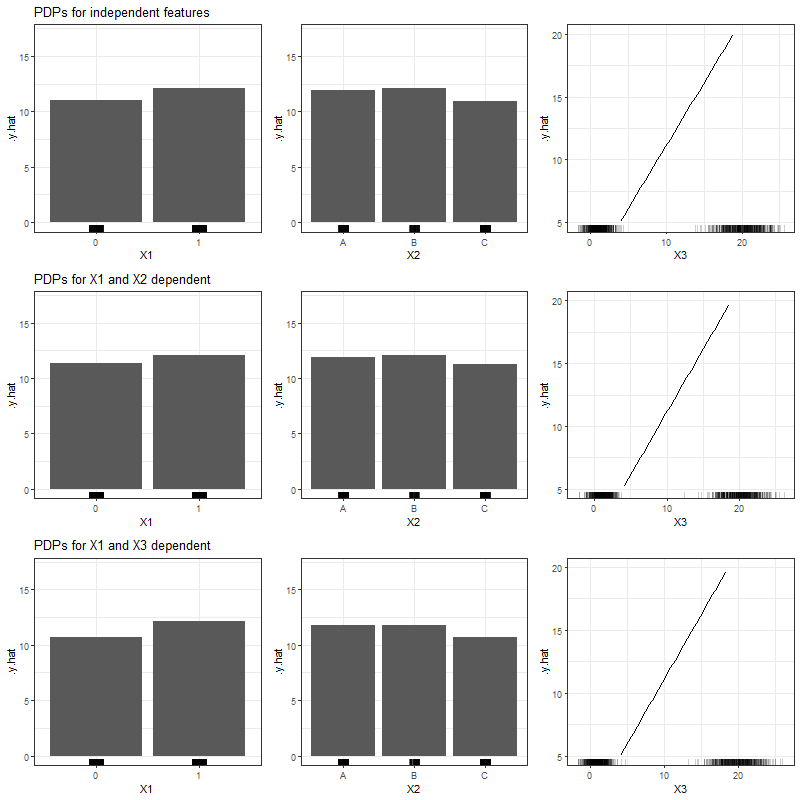
\includegraphics[width=1\linewidth]{images/VK_PDP_22_Set4_LM} \hfill{}

\caption{PDPs for categorical features $x_1$, $x_2$ and numerical feature $x_3$ (left to right), based on simulated data and LM as learning algorithm. Top row shows independent case, second row the case of two dependent categorical features and the bottom row the case of a numerical feature depending on a categorical feature.}\label{fig:Figure22}
\end{figure}

Apparently, the Linear Model is robust against our simulated
dependencies, since the PDPs of the correlated and dependent features do
not differ significantly from those of independent features.

\subsubsection{PDPs based on Random
Forest}\label{pdps-based-on-random-forest-3}

Figure \ref{fig:Figure23} shows the PDPs for all feature variables and
all simulation settings based on Random Forest.

\begin{figure}

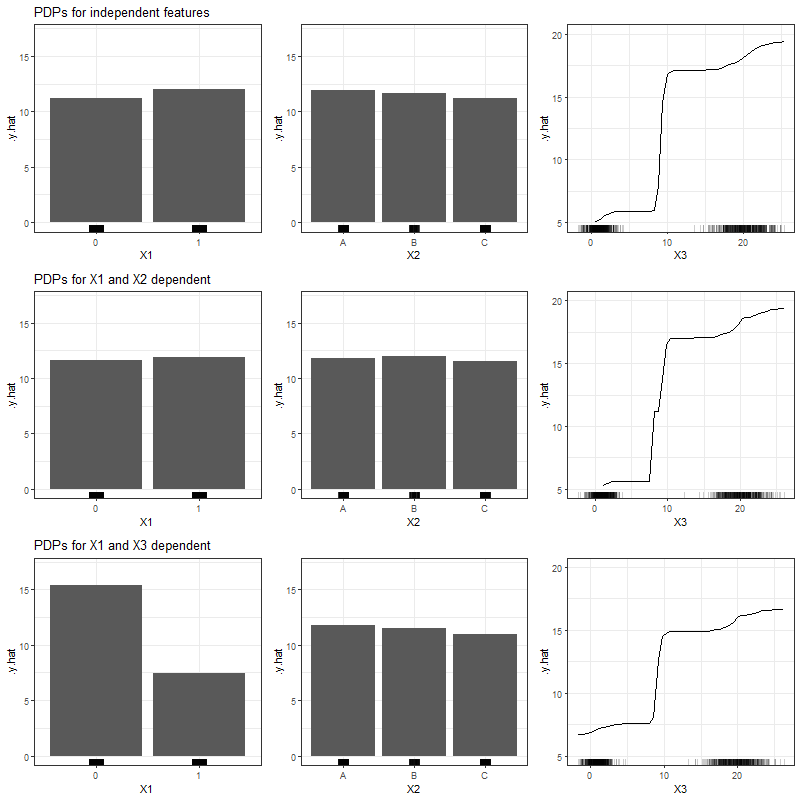
\includegraphics[width=1\linewidth]{images/VK_PDP_23_Set4_RF} \hfill{}

\caption{PDPs for categorical features $x_1$, $x_2$ and numerical feature $x_3$ (left to right), based on simulated data and RF as learning algorithm. Top row shows independent case, second row the case of two dependent categorical features and the bottom row the case of a numerical feature depending on a categorical feature.}\label{fig:Figure23}
\end{figure}

Based on Random Forest, the partial dependence function seems to be
impacted much stronger by our simulated dependencies, since the PDPs for
dependent variables indicate feature effects which differ from those in
the independent case. This is particularly true for a strong association
between a categorical an a numerical variable (bottom row of figure
\ref{fig:Figure23}).

\subsubsection{PDPs based on Support Vector
Machines}\label{pdps-based-on-support-vector-machines-3}

Figure \ref{fig:Figure24} shows the PDPs for all feature variables and
all simulation settings based on Support Vector Machines.

\begin{figure}

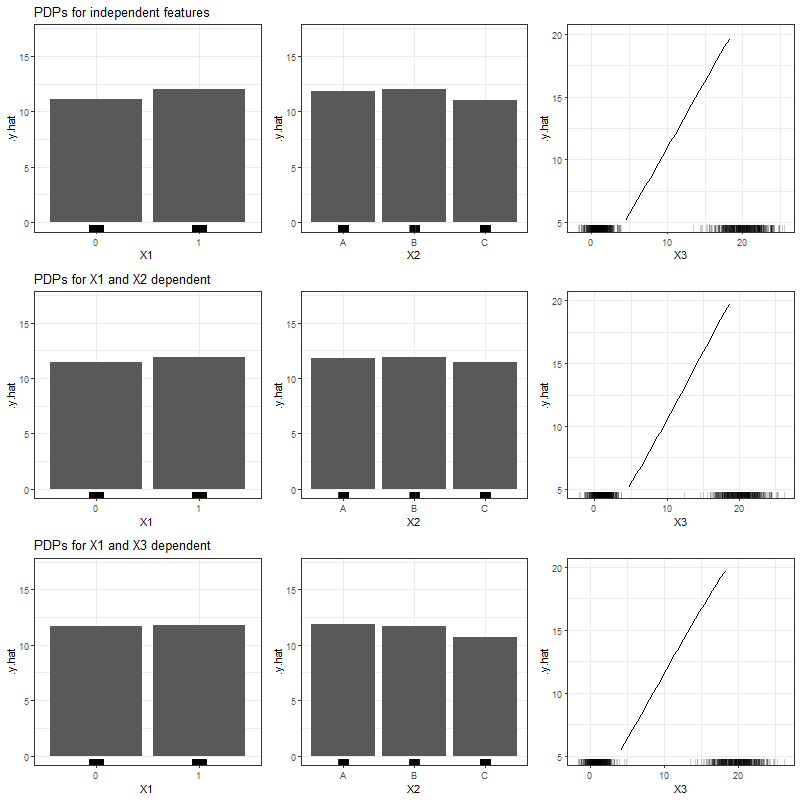
\includegraphics[width=1\linewidth]{images/VK_PDP_24_Set4_SVM} \hfill{}

\caption{PDPs for categorical features $x_1$, $x_2$ and numerical feature $x_3$ (left to right), based on simulated data and RF as learning algorithm. Top row shows independent case, second row the case of two dependent categorical features and the bottom row the case of a numerical feature depending on a categorical feature.}\label{fig:Figure24}
\end{figure}

In accordancy with our findings based on the Linear Model, the predicted
effects based on SVM seem to be robust against our simulated
dependencies, since the PDPs for the individual settings do not differ
significantly from the independent case.

\section{Extrapolation Problem: Simulation}\label{ExtrapolationProblem}

\subsection{Simulation based on established
learners}\label{ExtrapolationProblemEstablished}

In the problem description of this chapter we announced that, in
addition to the issue with dependent features, we want to investigate
the extrapolation problem and its implications for the computation of
partial dependence plots. For this purpose, we use the dataset
introduced in chapter \ref{ProblemDescription}, which was simulated once
with \(x_1\) and \(x_2\) independent, and once with both features
strongly correlated. Remember that in a next step, the observed data was
manipulated by cutting out all observations with
\(x_1 \in [0, 1.5] \wedge x_2 \in [0, 1.5]\), and thus artificially
producing an area with no observations (see figure \ref{fig:Figure02}).

Now we are looking at the PDPs resulting from these modifications.
Figure \ref{fig:Figure25} compares the PDP curves derived for both
features based on the complete, uncorrelated dataset to its manipulated
version with missing values.

\begin{figure}

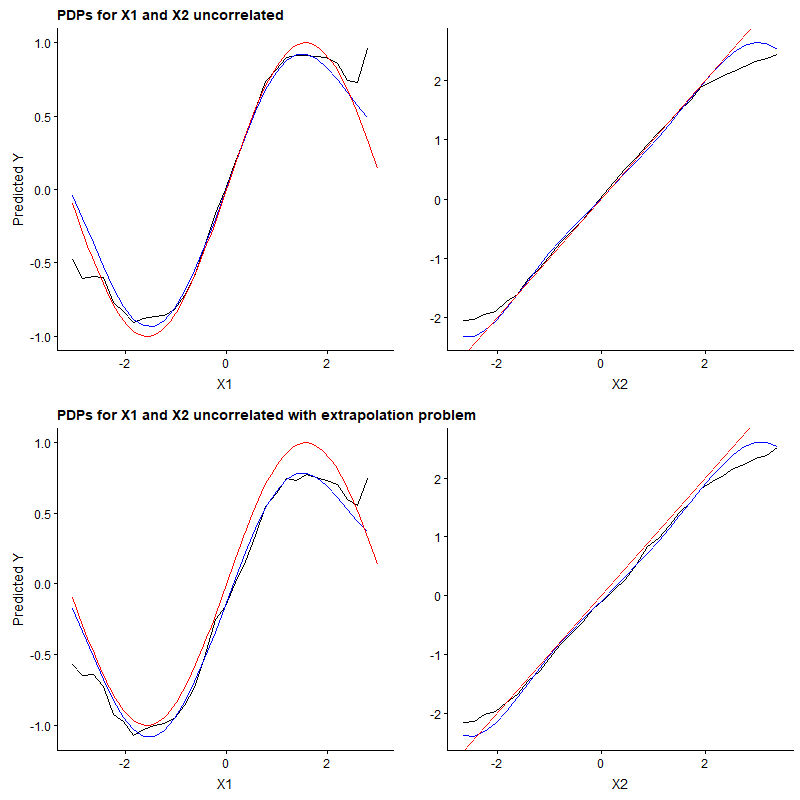
\includegraphics[width=0.9\linewidth]{images/VK_PDP_25_Extrapol_uncor} \hfill{}

\caption{PDPs for uncorrelated features $x_1$ (left) and $x_2$ (right) based on complete simulated dataset (top row) and based on manipulated dataset with missing observations (bottom row). The red curve represents the true effect of the feature for which the PDP is drawn, while the PDPs derived from the machine learning models are represented by curves drawn in black (Random Forest) and blue (SVM).}\label{fig:Figure25}
\end{figure}

The first row of PDPs in figure \ref{fig:Figure25}, computed on basis of
the complete dataset of uncorrelated features, adequately reflects the
true effects of \(x_1\) and \(x_2\) (red curves). In the presence of an
extrapolation problem, the adequacy of the predicted effects decreases.
Especially with the more complex, nonlinear effect of \(x_1\),
extrapolation causes a clearly visible deviation between the partial
dependence curves and the true feature effect, irrespective of the
learner.

In figure \ref{fig:Figure26} we do the same comparison, but this time
based on the dataset with strongly correlated features.

\begin{figure}

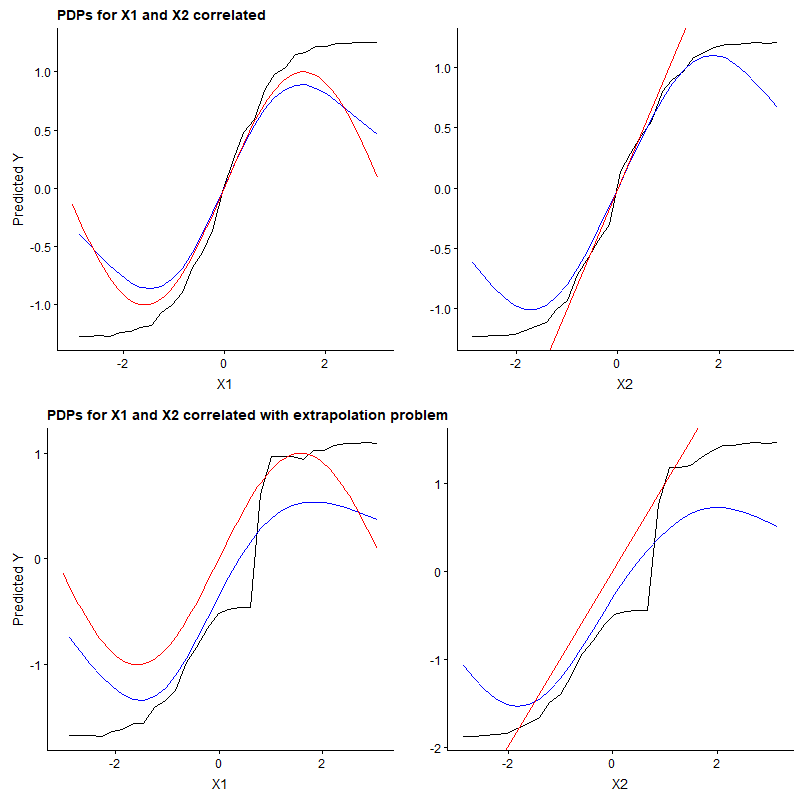
\includegraphics[width=0.9\linewidth]{images/VK_PDP_26_Extrapol_cor} \hfill{}

\caption{PDPs for correlated features $x_1$ (left) and $x_2$ (right) based on complete simulated dataset (top row) and based on manipulated dataset with missing observations (bottom row). The red curve represents the true effect of the feature for which the PDP is drawn, while the PDPs derived from the machine learning models are represented by curves drawn in black (Random Forest) and blue (SVM).}\label{fig:Figure26}
\end{figure}

From the first row of PDPs in figure \ref{fig:Figure26}, we again
discover the difficulty to obtain reliable PDPs when features are
dependent. The results in the bottom row of figure \ref{fig:Figure26}
are even more striking: with a combination of dependent features and
extrapolation, the PDPs come up with estimated effects which are far
from the true effects on the prediction. Those deviations seem to occur
irrespective of the learning algorithm.

\subsection{Simulation based on own prediction
function}\label{ExtrapolationProblemPrediction}

So far, all our analyses were based on the established learning
algorithms LM, RF and SVM. We have seen that the choice of the learner
does have an impact on the suitability of PDP curves. Obviously there is
a countless number of other possibilities to come up with prediction
functions other than the ones we have seen. PDPs are prone to fail when
this prediction function is doing `weird' stuff in areas outside the
feature distribution. This can happen due to the fact that the learner
minimizes the loss based on training data while there is no penalization
for extrapolation \citep{molnar2019}.

Let's illustrate the issue with an example. Assume we want to predict
the size of a potato (\(\hat{y}\)) by means of the share of maximum
amount of soil (\(x_1\)) and the share of maximum amount of water
(\(x_2\)) available during the process of growing the plant. The feature
variables are dependent in the sense that when using a larger amount of
soil, the farmer would also use a larger amount of water, i.e. \(x_1\)
and \(x_2\) are positively correlated. Typically, the more ressources
the farmer invests, the larger the crops. The corresponding model is
basically a simple linear regression which adds up the two components.

In the event of improper planting, meaning the usage of a too large
amount of water in proportion to the soil (and vice versa), the plant
would die and the result would be a potato of size 0. This is exactly
what our self-constructed prediction function predicts. Luckily, all
farmers in our dataset know how to grow potatoes, therefore there are no
such zero cases in the underlying observations. Figure
\ref{fig:Figure27} illustrates our observations as points and the
prediction function as shaded background colour.

\begin{figure}

{\centering 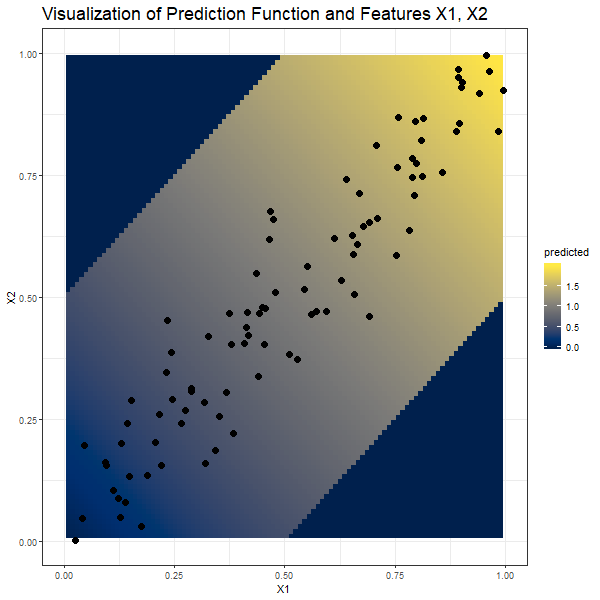
\includegraphics[width=0.6\linewidth]{images/VK_PDP_27_Prediction_Fct} 

}

\caption{Visualization of the observed data points (n=100) and the self-contructed prediction function. Dark blue background colour indicates a predicted potato size of zero which increases with the brightness of the yellow shaded background colour.}\label{fig:Figure27}
\end{figure}

In view of the observed data, one would expect to uncover a linear
effect of both feature variables when looking at the corresponding PDPs.
As we can see in figure \ref{fig:Figure28}, this is not necessarily the
case. While the two-dimensional PDP perfectly depicts the prediction
function, the individual PDPs for feature \(x_1\) and \(x_2\) fail in
the areas where the prediction function does `weird' stuff compared to
what has been observed.

\begin{figure}

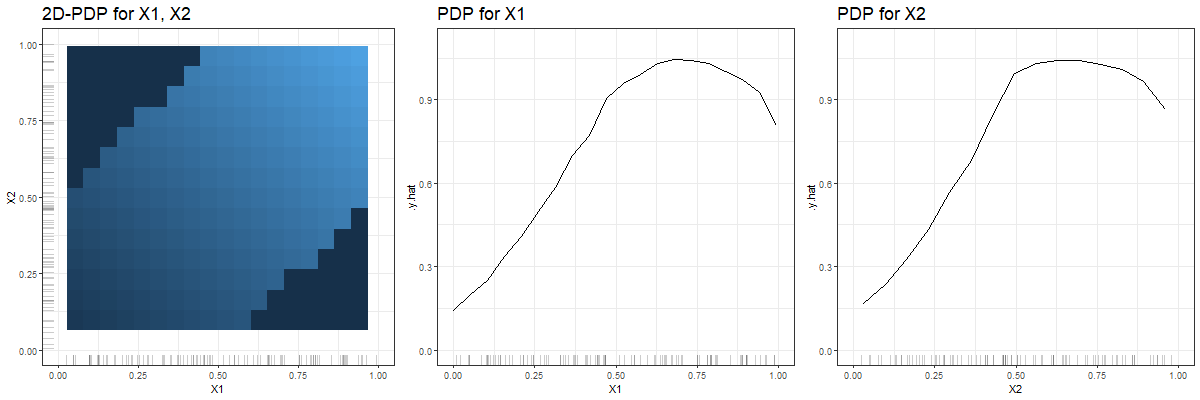
\includegraphics[width=1.1\linewidth]{images/VK_PDP_28_Prediction_Fct_Fail} \hfill{}

\caption{The first plot shows the two-dimensional PDP for features $x_1$ and $x_2$. The darker the background colour, the smaller the predicted values. The other plots are the PDPs derived for feature $x_1$ and $x_2$ respectively. Up to a value of approximately 0.5 both partial dependence curves are mostly linear and bend at larger $x_1$- / $x_2$-values.}\label{fig:Figure28}
\end{figure}

\section{Summary}\label{summary}

Our analysis of partial dependence plots in the context of dependent
features and missing values has revealed that both a violation of the
underlying independence assumption and the presence of areas with no
observations can have a significant impact on the marginalized feature
effects. As a consequence, there is a risk of misinterpretation of the
effect of features in \(x_S\). Hooker and Mentch (2019) propose to make
use of local explanation methods in order to avoid extrapolation. ICE
plots, as an example, can be restricted to values in line with the
distribution of observed data. However, the authors also point out that
this approach cannot serve as a global representation of the learned
model \citep{2019arXiv190503151H}.

In our simulations, we have also seen cases where the PDP (or the
underlying machine learning algorithm) proved to be relatively robust
against the dependency of features. Further to the independence
assumtion, there are also other parameters playing a role for the
accuracy of PDPs, like the grid size, the number of observations, the
learning algorithm, variance in the data, complexity of the data
generating process, etc.

In practical applications it is recommended to analyse the variables
used in the model, both by means of correlation and/or association
measures and content-wise in liason with experts having domain
knowledge. Furthermore, data scientists can apply methods based on the
conditional expectation, such as M-plots or ALE plots. The concept and
limitations of the latter will be discussed in chapters 6-8 of this
book.

\chapter{PDP and Causal Interpretation}\label{pdp-causal}

\emph{Author: Thommy Dassen}

\emph{Supervisor: Gunnar König}

\section{Introduction}\label{introduction-1}

Machine learning methods excel at learning associations between features
and the target. The supervised machine learning model estimates \(Y\)
using the information provided in the feature set \(X\). Partial
dependence plots (PDPs) allow us to inspect the learned model. We can
analyze how the model prediction changes given changes in the features.

The unexperienced user may be tempted to transfer this insight about the
model into an insight in the real world. If our model's prediction
changes given a change on some feature \(X_j\), can we change the target
variable \(Y\) in the real world by performing an intervention on
\(X_j\)?

Of course, this is not generally true. Without further assumptions we
cannot interpret PDPs causally (like we cannot interpret coefficients of
linear models causally). Curiously, certain assumption sets still allow
for a causal interpretation.

In this Chapter we will elaborate on specific assumptions sets that
allow causal interpretation and will empirically evaluate the resulting
plots. We therefore assume certain data generating mechanisms, also
referred to as structural equation models (SEMs), and use Judea Pearl's
do-calculas framework to compute the true distributions under an
intervention, allowing to e.g.~compute the average causal effect. Graphs
are used to visualize the underlying dependence structure. We will see
scenarios in which the PDP gives the same result as an intervention and
scenarios in which the limitations of the PDP as a tool for causal
interpretation become clear.

To interpret causally means to interpret one state (the effect) to be
the result of another (the cause), with the cause being (partly)
responsible for the effect, and the effect being partially dependent on
the cause. \citep{zhaohastie} formulated three elements that are needed
to ensure that the PDP coincides with the intervention effect:\\
1. A good predictive model which closely approximates the real
relationship.\\
2. Domain knowledge to ensure the causal structure makes sense and the
backdoor criterion, explained below, is met.\\
3. A visualization tool like a PDP (or an Individual Conditional
Expectation plot)

The first condition is an important one, because there is a big
difference between being able to causally interpret an effect for the
\emph{model} and using it as a causal interpretation for the real world.
The second condition will make clear when PDPs are the same, and when
they are different from interventions on the data. In this chapter we
will systematically analyze a number of scenarios in order to see under
which conditions PDPs can be causally interpreted or not.

\section{Motivation}\label{motivation}

Before we have a look at various scenarios and settings involving
interventions, let's look at an exemplary problem. Let's say we have a
dataset containing data on the amount of ice-cream consumption per
capita and the temperature outside. The temperature is causal for the
ice-cream consupmtion: People eat more ice-cream when temperatures are
high than when temperatures are low. Therefore, both quantities are
dependent as well. A statistical model learns to use the information in
one of the variables to predict the other, as is evident in the plots
below.

\begin{figure}

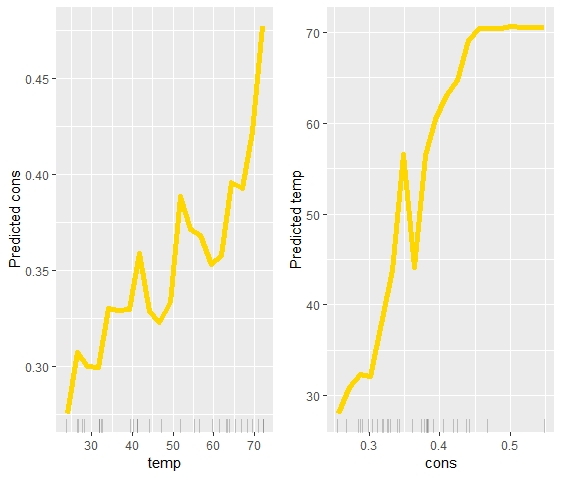
\includegraphics[width=1\linewidth]{images/ice_cream} \hfill{}

\caption{The PDP on the left shows temperature causing ice-cream consumption. The PDP on the right shows ice-cream consumption causing temperatures. Which one is correct?}\label{fig:Figure1}
\end{figure}

While the dependence is learned correctly, it would be wrong to
interpret the second plot causally. When more ice cream is consumed, it
is likely that the temperature is higher. However, consuming more ice
cream will not change the amount of ice cream that is being eaten.

This example illustrates the gap between predictive models and causal
models. Without further assumptions we cannot interpret effects of
changes in features on the model prediction as effects that would be
present in the real world. In this simple scenario it is quite clear in
which cases a causal interpretation is clear. However, in more
complicated scenarios a more elaborate formalization of assumptions
under which a causal interpretation is possible are helpful. We will
analyze this theoretically in the next section and will empirically
evaluate the theoretical findings.

It may be noted that other problems can occur when using PDPs for model
interpretation. E.g. as shown by \citep{scholbeck}, assume we have data
that is distributed as follows:

\[ Y \leftarrow  X_{1}^2 - 15X_{1}X_2 + \epsilon \]
\[ X_1 \sim \mathcal{U}(-1, 1), \ \ \ \ \ X_2 \sim \mathcal{U}(-1, 1), \ \ \ \ \ \epsilon \sim \mathcal{N}(0,0.1), \ \ \ \ \ N \leftarrow 1000    \]
Training a Random Fordest on this data leads to Figure \ref{fig:Figure2}
below. Looking at the PDP, one would assume that \(X_1\) has virtually
no impact on \(Y\). The ICE curves, however, show that the averaging
effect of the PDP completely obfuscates the true effect, which is highly
positive for some observations while being highly negative for others.
In this example too it would be misguided to simply interpret the PDP
causally and state that \(X_1\) does not have any impact on \(Y\)
whatsoever. This may capture the average effect correctly, but evidently
not true on the individual level.

\begin{figure}

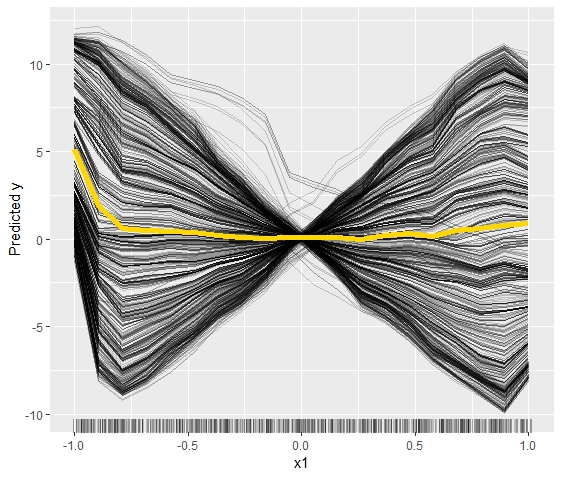
\includegraphics[width=1\linewidth]{images/avg_vs_individual} \hfill{}

\caption{The average effect of the PDP (yellow line) hides the heterogeneity of the individual effects }\label{fig:Figure2}
\end{figure}

\section{Causal Interpretability: Interventions and Directed Acyclical
Graphs}\label{causal-interpretability-interventions-and-directed-acyclical-graphs}

For the rest of the Chapter we will assume we know the structure of the
mechanisms are underlying our dataset to derive assumptions under which
a causal interpretation is possible. With the help of Pearl's
do-calculus \citep{pearl1993} we can compute the true causal effect of
interventions. Pearls do-calculus relies on an underlying Structural
Equation Model, the structure of which can be visualized with causal
graphs. In the structural equation model this is equivalent to removing
all incoming dependencies for the intervened variable and fixing a
specified value. As an effect, the distributions of variables that are
caused by the intervened variable may change as well. For more details
refer to \citep{pearl1993}. It is important to recognize that an
intervention is different from conditioning on a variable. Therefore the
difference between a variable \(X\) taking a value \(x\) naturally and
having a fixed value \(X=x\) is reflected in the notation. The latter is
denoted by \(do(X=x)\). As such, \(P(Y=y|X=x)\) is the probability that
\(Y=y\) conditional on \(X=x\). \(P(Y=y|do(X=x))\) is then the
population distribution of \(Y\) if the value of \(X\) was fixed at
\(x\) for the entire population.

In order to avoid complex scenarios (dynamical models, equilibrium
computation) we restrict ourselves to causal structures that can be
visualized with Direct Acyclical Graphs. A DAG is a representation of
relationships between variables in graphical form. Each variable is
represented as a \emph{node} and the lines between these nodes, or
\emph{edges}, show the direction of the causal relationship through
arrowheads. In addition to being directed, these graphs are per
definition acyclical. This means that a relationship
\(X \rightarrow Y \rightarrow Z \rightarrow X\) can not be represented
as a DAG. Several examples of DAGs follow in the rest of the chapter, as
each scenario starts with one. With regards to interventions, in a
graphical sense this simply means removing edges from direct parents to
the variable.

In order to know when a causal interpretation makes sense, more is
needed than only a representation of a DAG and knowledge of how to do an
intervention. An important formula introduced by \citep{pearl1993}
adresses exactly this problem: The back-door adjustment formula. This
formula stipulates that the causal effect of \(X_S\) on \(Y\) can be
identified if the causal relationship between the variables can be
visualized in a graph and \(X_C\), the complementary set to \(X_S\),
adheres to what he called the back-door criterion. The back-door
adjustment formula is:

\[P(Y|do(X_S = x_S)) = \int P(Y |X_S = x_S, X_C = x_C) dP(x_C)\] As
\citep{zhaohastie} pointed out, this formula is basically the same as
the formula for the partial dependence of \(g\) on a subset of variables
\(X_S\) given output \(g(x)\):

\[ g_S(x_S) = \mathbb E_{x_C}[g(x_S, X_C)] = \int g(x_S, x_C)dP(x_C)  \]
If we take the expectation of Pearl's adjustment formula we get:
\[ E[Y |do(X_S = x_S)] = \int E[Y |X_S = x_S, X_C = x_C] dP(x_C) \]
These last two formulas are the same, if \(C\) is the complement of
\(S\).

\citep{pearl1993} defined a back-door criterion that needs to be
fulfilled in order for the adjustment formula to be valid. It states
that:

\begin{enumerate}
\def\labelenumi{\arabic{enumi}.}
\item
  No node in \(X_C\) can be a descendant of \(X_S\) in the DAG \(G\).
\item
  Every ``back-door'' path between \(X_S\) and \(Y\) has to be blocked
  by \(X_C\).
\end{enumerate}

\section{Scenarios}\label{scenarios}

After these two introductory problems of PDPs, the rest of this chapter
will look at PDPs through the causal framework of \citep{pearl1993}.
This means we will look at various causal scenarios visualized through
DAGs and compare the PDPs created under this structure with the actual
effect of interventions.

In each scenario nine settings will be simulated for PDP creation,
consisting of three standard deviations for the error term (0.1, 0.3 and
0.5) and three magnitudes of observations (100, 1000, 10000).
Furthermore, each setting for the PDP was simulated across twenty runs.
Each of the nine plots will therefore show twenty PDPs in order to give
a solid view of the relationship the PDPs capture for each setting. In
addition to the plots of the PDPs, which will be the first three columns
in each figure, the actual effect under intervention will be shown in a
fourth column as a single yellow line. The true intervention effects
(column 4) were all simulated with a thousand observations. Initial
tests resulted in a large increase in computation time with a higher
number of observations, but with results that hardly differed from those
obtained with one thousand observations. For reasons of computational
efficiency, we only use out of the box random forest models. In future
work, other model classes and hyperparameter settings should be
considered, e.g.~by using approaches from automatic machine learning.

The process for obtaining the intervention curve was as follows: Let
\(X\) be the predictor variable of interest with possible values
\(x_{1}, x_{2}, x_{n}\) and \(Y\) the response variable of interest. for
each unique \(i \in \{1,2,\dots,n\}\) do\\
(1) make a copy of the data set\\
(2) replace the original values of \(X\) with the value \(X_{(i)}\) of
\(X\) under intervention\\
(3) recompute all variables dependent on \(X\) using the replacement
values as input. This includes \(Y\), but potentially also other
features that rely on \(X\) for their value. Note that only \(X\) is
replaced with \(X_i\) in the existing equations. Both the equations and
error terms remain the same as before.\\
(4) Compute the average \(Y_i\) in dataset \(i\) given \(X_i\).\\
(5) (\(X_i\), \(Y_i\)) are a single point on the intervention curve.

\textbf{Scenario 1: }

\begin{figure}
\centering
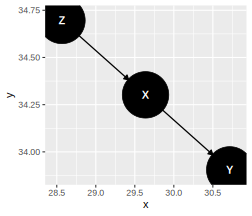
\includegraphics{book_files/figure-latex/Figure3-1.pdf}
\caption{\label{fig:Figure3}Chain DAG where X has a direct impact on Y, but
is dependent on Z}
\end{figure}

In the first scenario, we have a chain DAG, seen in Figure
\ref{fig:Figure3}. Our variable \(X\) is impacted by \(Z\) and has a
direct effect on \(Y\). \(Z\), however, does not. \(X_C\) consists of
\(Z\), which is not a descendant of \(X\). There is also no backdoor
path between \(X\) and \(Y\). The backdoor criterion is met. In this
scenario the expectation is thus that the PDPs should be overall equal
to the true intervention. The initial simulation settings for this
scenario are as follows:

\[ Y \leftarrow X + \epsilon_Y  \]
\[ \epsilon_X,\epsilon_Y ~ \sim \mathcal{N}(0, 0.1), \ \ \ \ \ \epsilon_Z \sim \mathcal{U}(-1,1),\ \ \ \ \ Z \leftarrow \epsilon_Z, \ \ \ \ \ X \leftarrow Z + \epsilon_X, \ \ \ \ \ N \leftarrow 100 \]

As will be done in all scenarios, both standard deviaton for
\(\epsilon\) and \(N\) were varied across 3 levels leading to 9
settings.

\begin{figure}

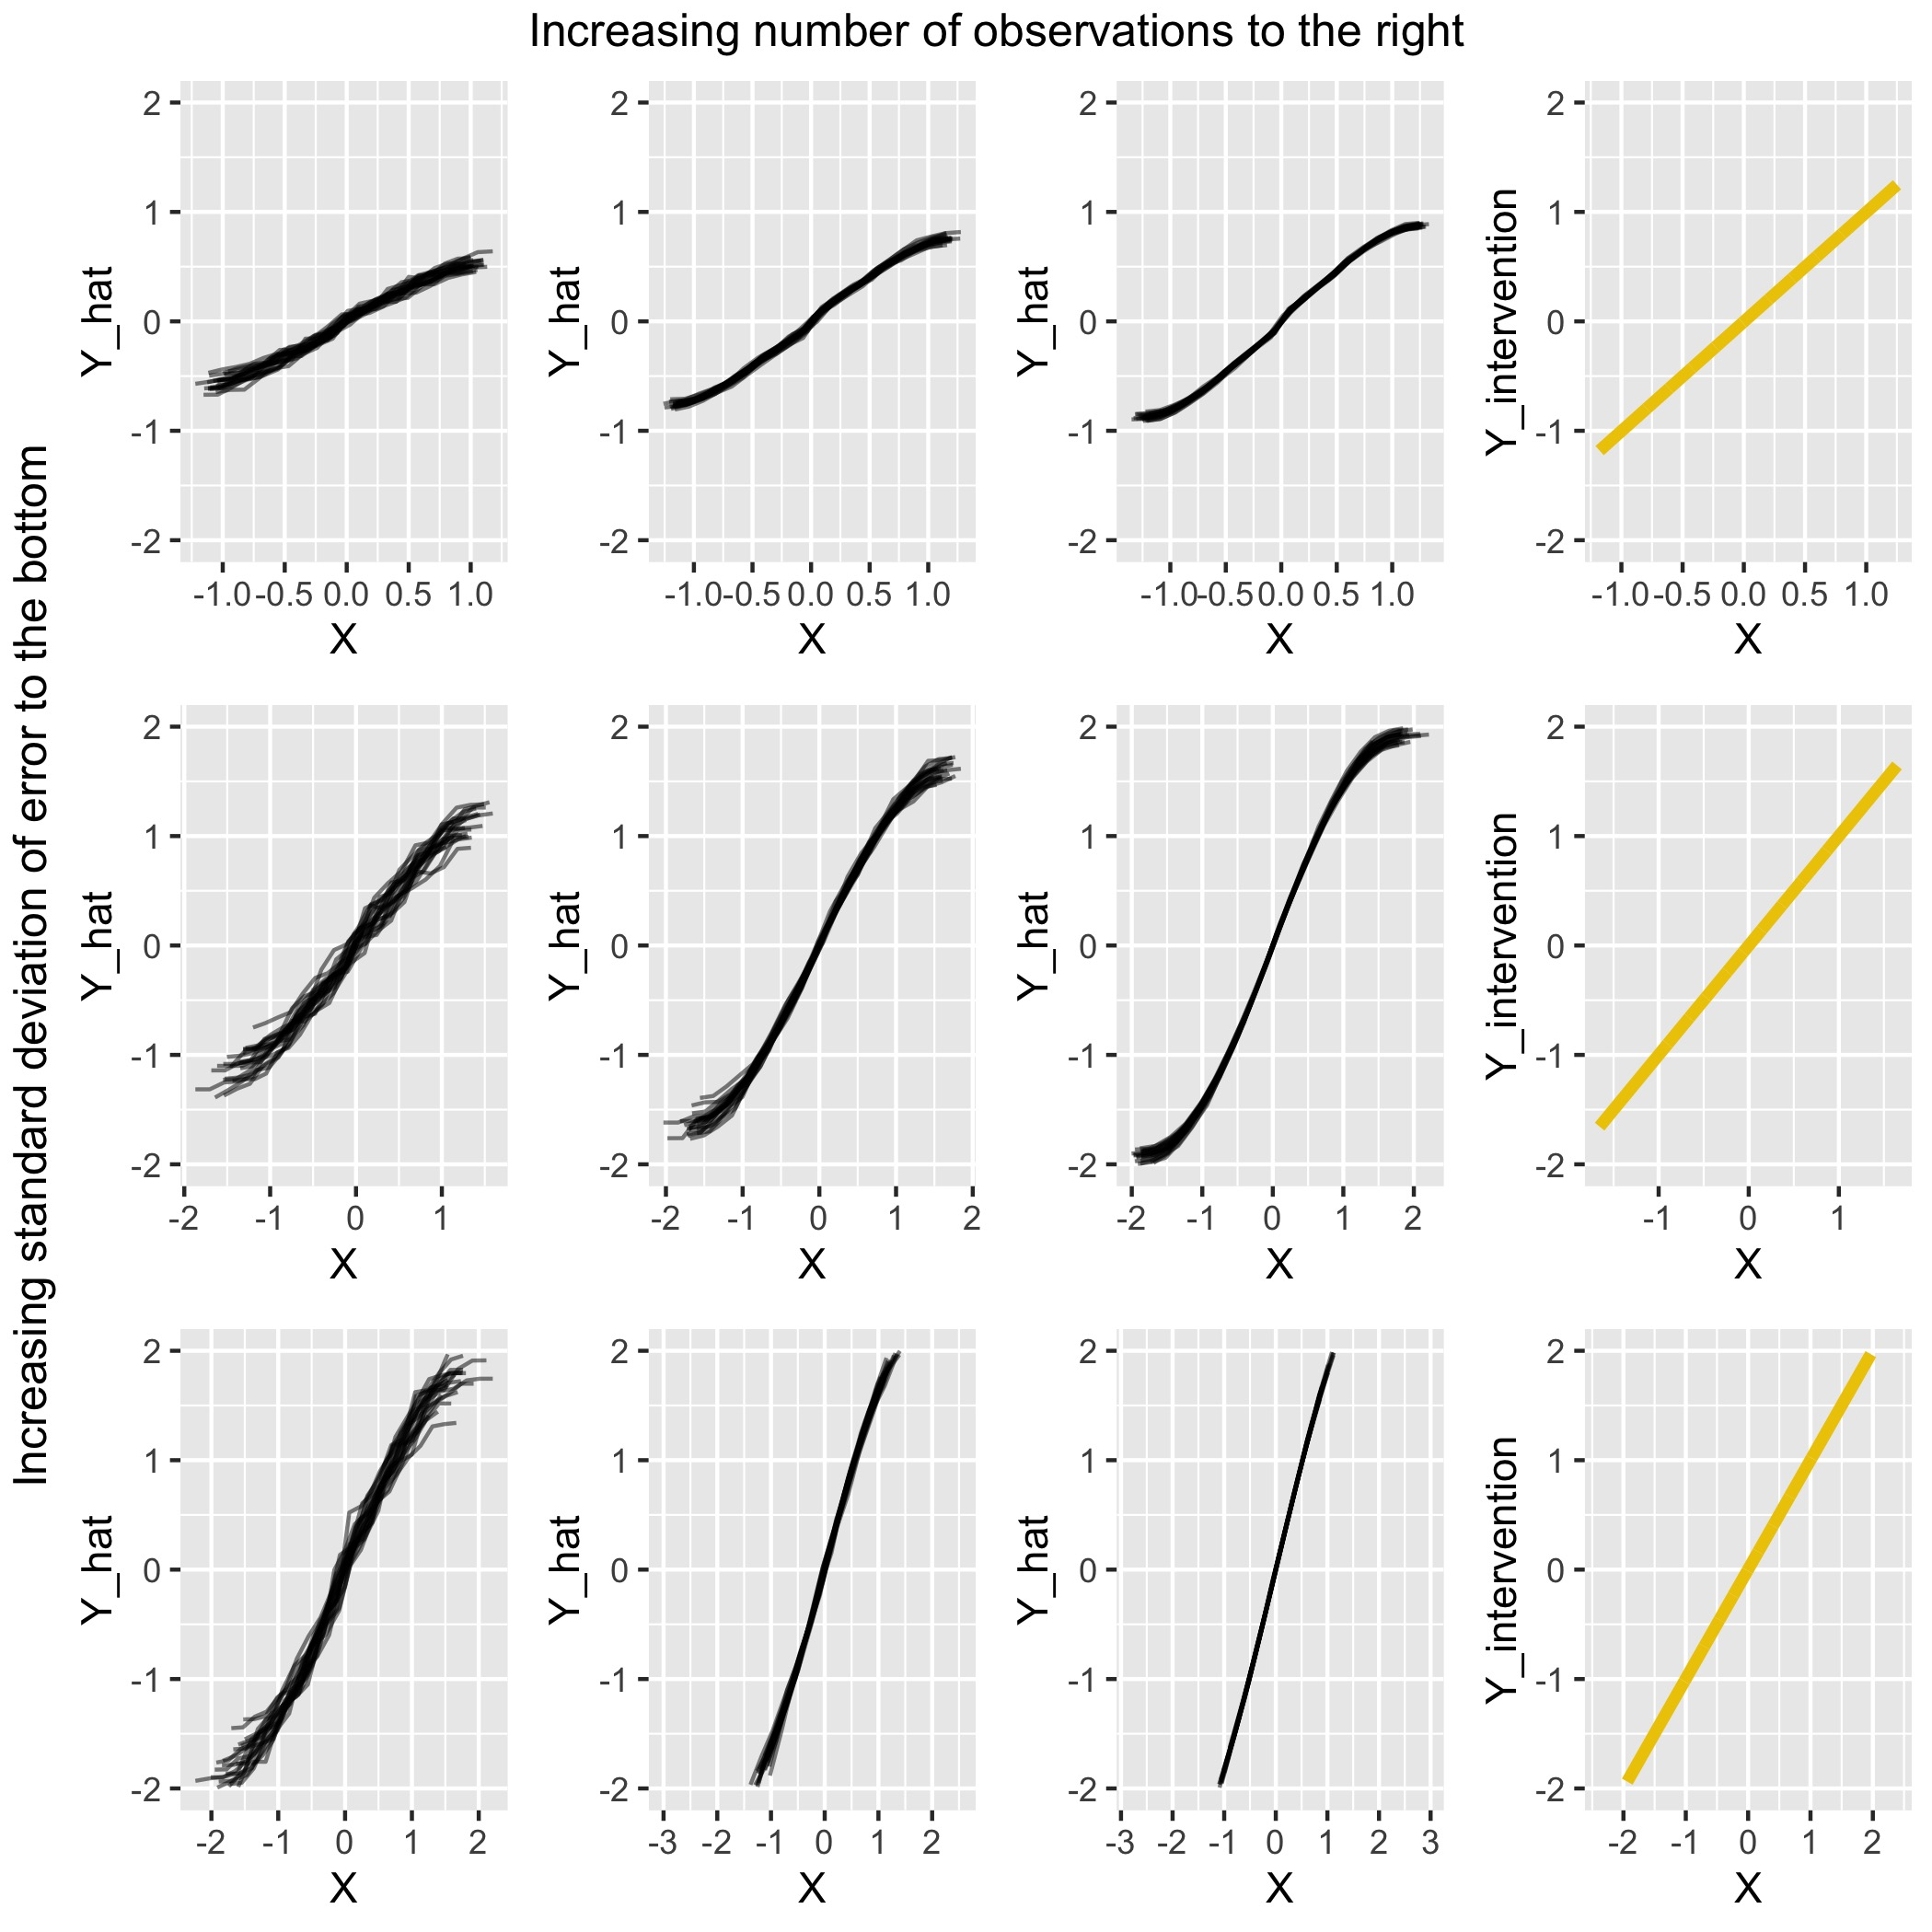
\includegraphics[width=1\linewidth]{images/scenario1_all} \hfill{}

\caption{Comparison for scenario 1 of PDPs under various settings with the (yellow) intervention curve on the right}\label{fig:Figure4}
\end{figure}

Overall the PDPs match the intervention curves fairly well. Outside of
the extreme regions of \(X\), where some curvature is present, the
linear quality of the intervention curve is evident in the PDPs.
Furthermore, the scale of \(\hat{Y}\) is comparable to the scale of
\(Y_{intervention}\) in most settings.

\textbf{Scenario 2: Chain DAG}

\begin{figure}
\centering
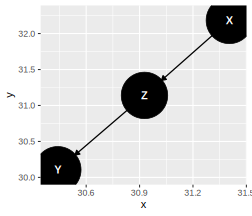
\includegraphics{book_files/figure-latex/Figure5-1.pdf}
\caption{\label{fig:Figure5}Chain DAG where X has no a direct impact on Y,
but only indirectly through Z}
\end{figure}

In this scenario the DAG again looks like a chain. \(X\) has an effect
on \(Y\) through \(Z\), but no direct relationship between \(X\) and
\(Y\) exists. Note that since \(Z\) is a descendant of \(X\), the PDP
and intervention curve should not coincide. The initial simulation
settings for this scenario are as follows:

\[ Y \leftarrow Z + \epsilon_Y  \]
\[ \epsilon_Y,\epsilon_Z ~ \sim \mathcal{N}(0, 0.1), \ \ \ \ \ \epsilon_X \sim \mathcal{U}(-1,1), \ \ \ \ \ X \leftarrow \epsilon_X, \ \ \ \ \ Z \leftarrow X + \epsilon_Z, \ \ \ \ \ N \leftarrow 100 \]

\begin{figure}

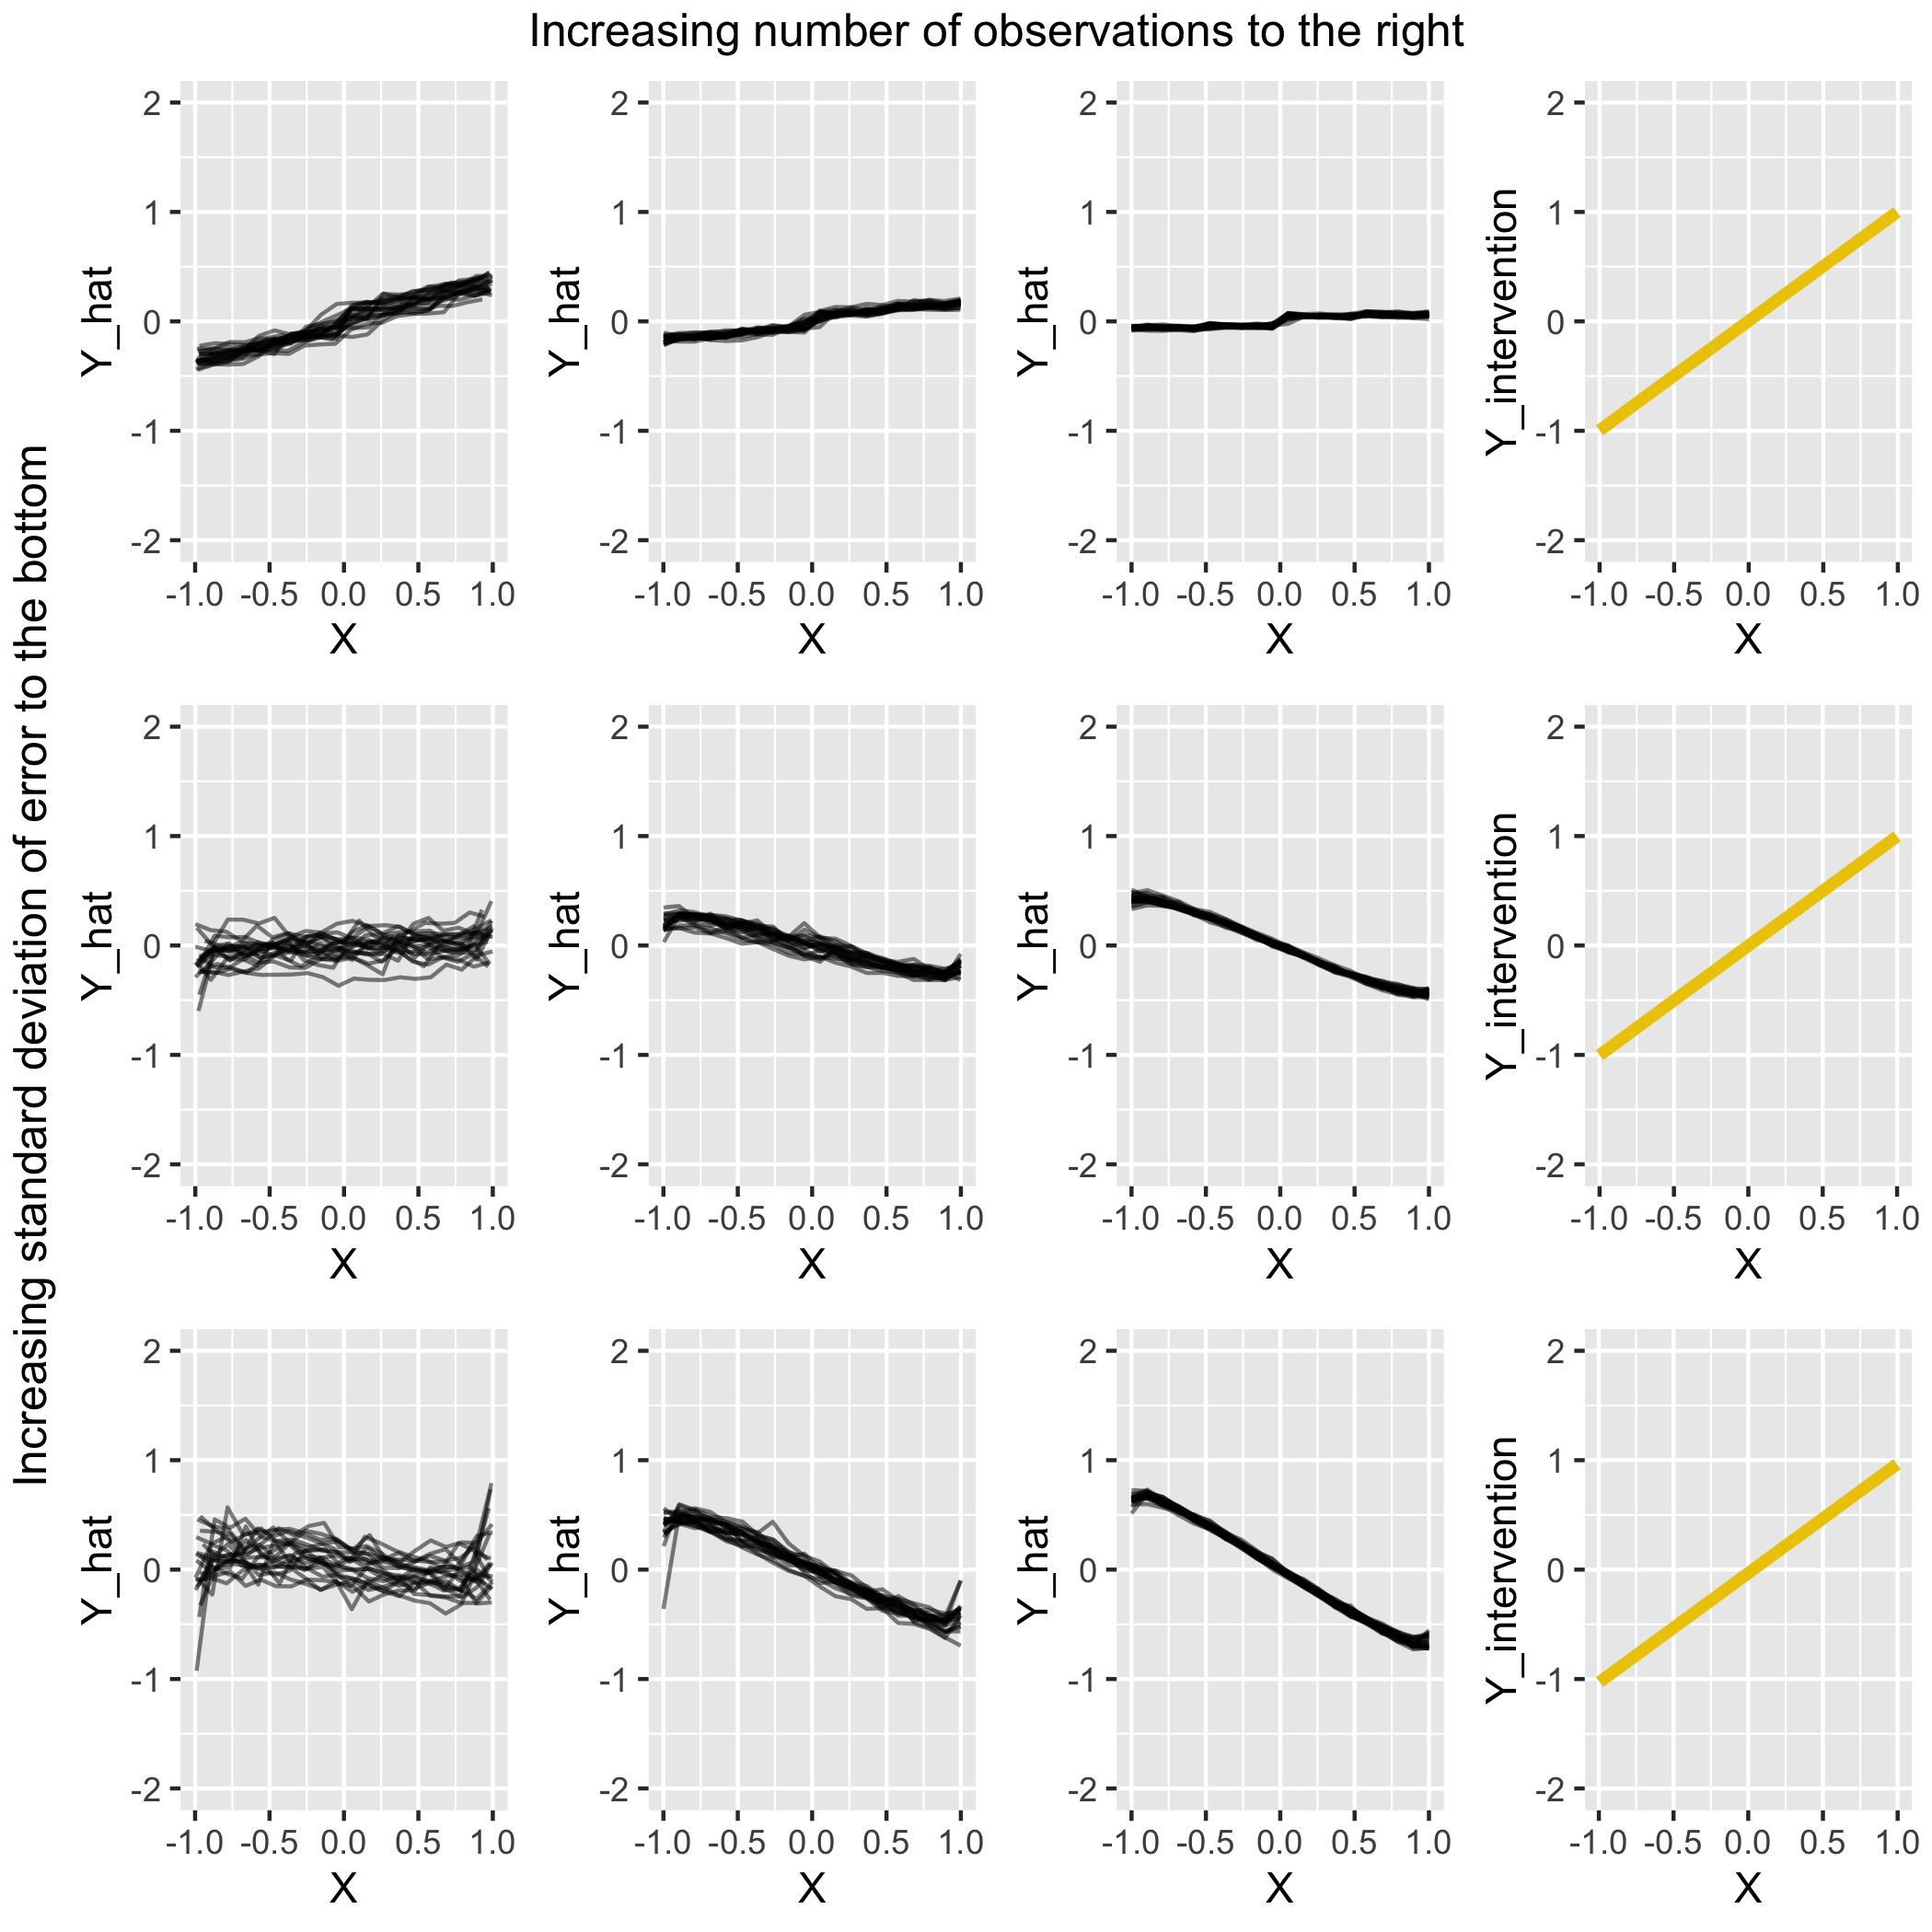
\includegraphics[width=1\linewidth]{images/scenario2_all} \hfill{}

\caption{Comparison for scenario 2 of PDPs under various settings with the (yellow) intervention curve on the right}\label{fig:Figure6}
\end{figure}

As can be seen from Figure \ref{fig:Figure6}, the PDP plots do not match
the intervention plots well in several cases. The effect strength is a
lot smaller and in fact, four out of nine settings show a negative slope
for the relationship between \(X\) and \(Y\) in comparison to the
overall positive slope for the true intervention. The first row performs
best, as expected due to the relatively small error that is used.
Interesting is also that in the second and third row, where the error
has been increased, the PDP slope goes from positive to negative between
the first and second column. PDP accuracy thus suffers in situations
where the observation count is low. In theory, we would expect the slope
to be zero. It remains to be investigated why we still see a trend, and
why this trend is negative in some cases.

\textbf{Scenario 3}

After two chains, we now have a scenario where \(X\) has an influence on
both \(Z\) and \(Y\) directly, as well as \(Z\) having an impact on
\(Y\), as seen in Figure \ref{fig:Figure7}. X confounds
\(Z \rightarrow Y\) here. An example of a confounding variable in real
life might be for instance the relationship between the \emph{level of
physical activity} and \emph{weight gain}, which is confounded by
\emph{age}. \emph{Age} affects both \emph{weight gain} and the
\emph{level of physical activity} (on average), making it similar to the
X in our scenario here. This scenario is similar to the previous one
with only an edge between \(X\) and \(Y\) having been added. As can be
seen from the DAG in \ref{fig:Figure7}, \(Z\) is still a descendant of
\(X\). As the backdoor criterion is not met, we cannot expect a causal
interpretation to be valid.

\begin{figure}
\centering
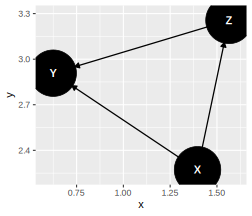
\includegraphics{book_files/figure-latex/Figure7-1.pdf}
\caption{\label{fig:Figure7}X is a confounding variable impacting both Z and
Y}
\end{figure}

The similarity to the previous scenario can also be noted in the
simulation settings, where the only difference is the addition of \(X\)
to the equation for \(Y\).

\[ Y \leftarrow Z + X + \epsilon_Y  \]
\[ \epsilon_Y,\epsilon_Z ~ \sim \mathcal{N}(0, 0.1), \ \ \ \ \ \epsilon_X \sim \mathcal{U}(-1,1), \ \ \ \ \ X \leftarrow \epsilon_X, \ \ \ \ \ Z \leftarrow X + \epsilon_Z, \ \ \ \ \ N \leftarrow 100 \]

\begin{figure}

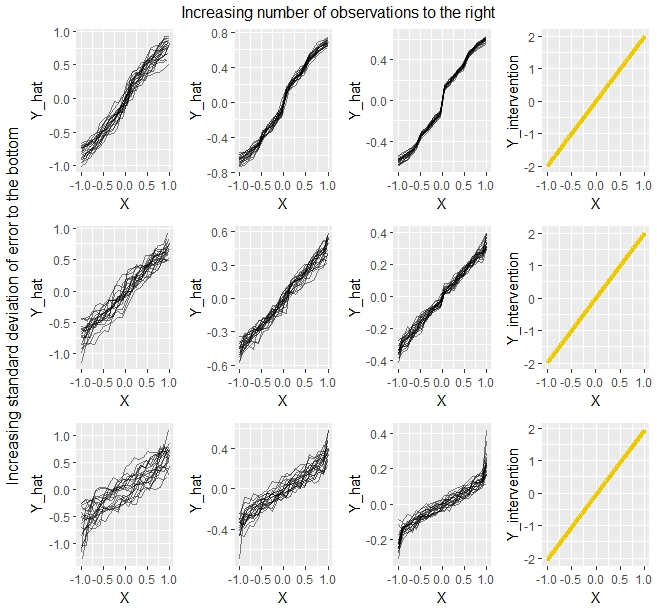
\includegraphics[width=1\linewidth]{images/scenario3_all} \hfill{}

\caption{Comparison for scenario 3 of PDPs under various settings with the (yellow) intervention curve on the right}\label{fig:Figure8}
\end{figure}

The expectation was that the PDP would not show the same results as the
true intervention. On first glance in Figure \ref{fig:Figure8}, the PDPs
do not seem to be as inaccurate as they were in scenario 2. An overall
upward trend seen in the true intervention on the right is also captured
by the PDPs in all settings. However, big differences do exist. First of
all, the scale of \(\hat{Y}\) is off in every setting. This issue gets
worse both when the standard deviation of the error increases and when
the number of observations is increased. The worst setting is the bottom
right, where \(N = 10.000\) and the standard deviation of the error is
0.5. The range of \(\hat{Y}\) is very small compared to the true
intervention next to it and the slope is not steep enough. In fact, the
correct slope can only be seen in a very few points: In the top row plot
2 and 3 around \(X=0\) and on the second row plot 3, also around
\(X=0\). Overall the result is not as poor as in scenario 2, but a
causal interpretation of these plots would lead to a severe
underestimation of the impact \(X\) has on \(Y\).

\textbf{Scenario 4}

Scenario 4 consists of a direct effect of \(X\) on \(Y\). \(Z\)
meanwhile is unrelated to both \(X\) and \(Y\). It is however included
in the simulation and included in the model that is run to create the
PDPs. In a non-simulated setting, \(Z\) can be seen as a variable that
we assume might be related to \(Y\) and therefore include, but in
actuality has nothing to do with the causal process and should not be
included. We will see now how the PDP deals with this kind of variable
in the mix.

\begin{figure}

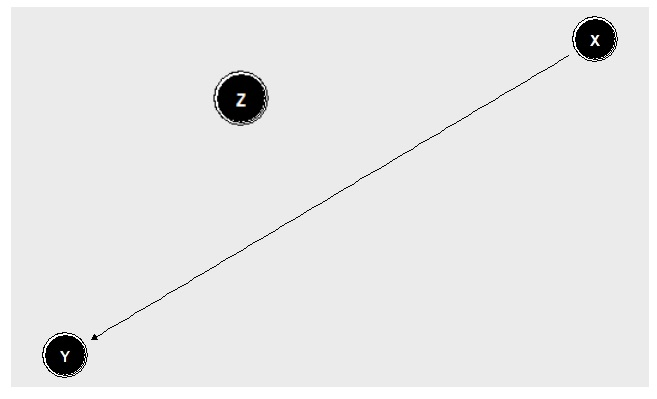
\includegraphics[width=1\linewidth]{images/scenario4} \hfill{}

\caption{X directly impacts Y. Z is included in our model, but has no relationship to X or Y}\label{fig:Figure9}
\end{figure}

For the simulation the initial settings look as follows, again
increasing both the standard deviation of the error and the magnitude of
observations from this starting point.
\[ Y \leftarrow X + \epsilon_Y  \]
\[ \epsilon_Y ~ \sim \mathcal{N}(0, 0.1), \ \ \ \ \ \epsilon_X, \epsilon_Z \sim \mathcal{U}(-1,1), \ \ \ \ \ X \leftarrow \epsilon_X,\ \ \ \ \ Z \leftarrow \epsilon_Z, \ \ \ \ \ N \leftarrow 100 \]

\begin{figure}

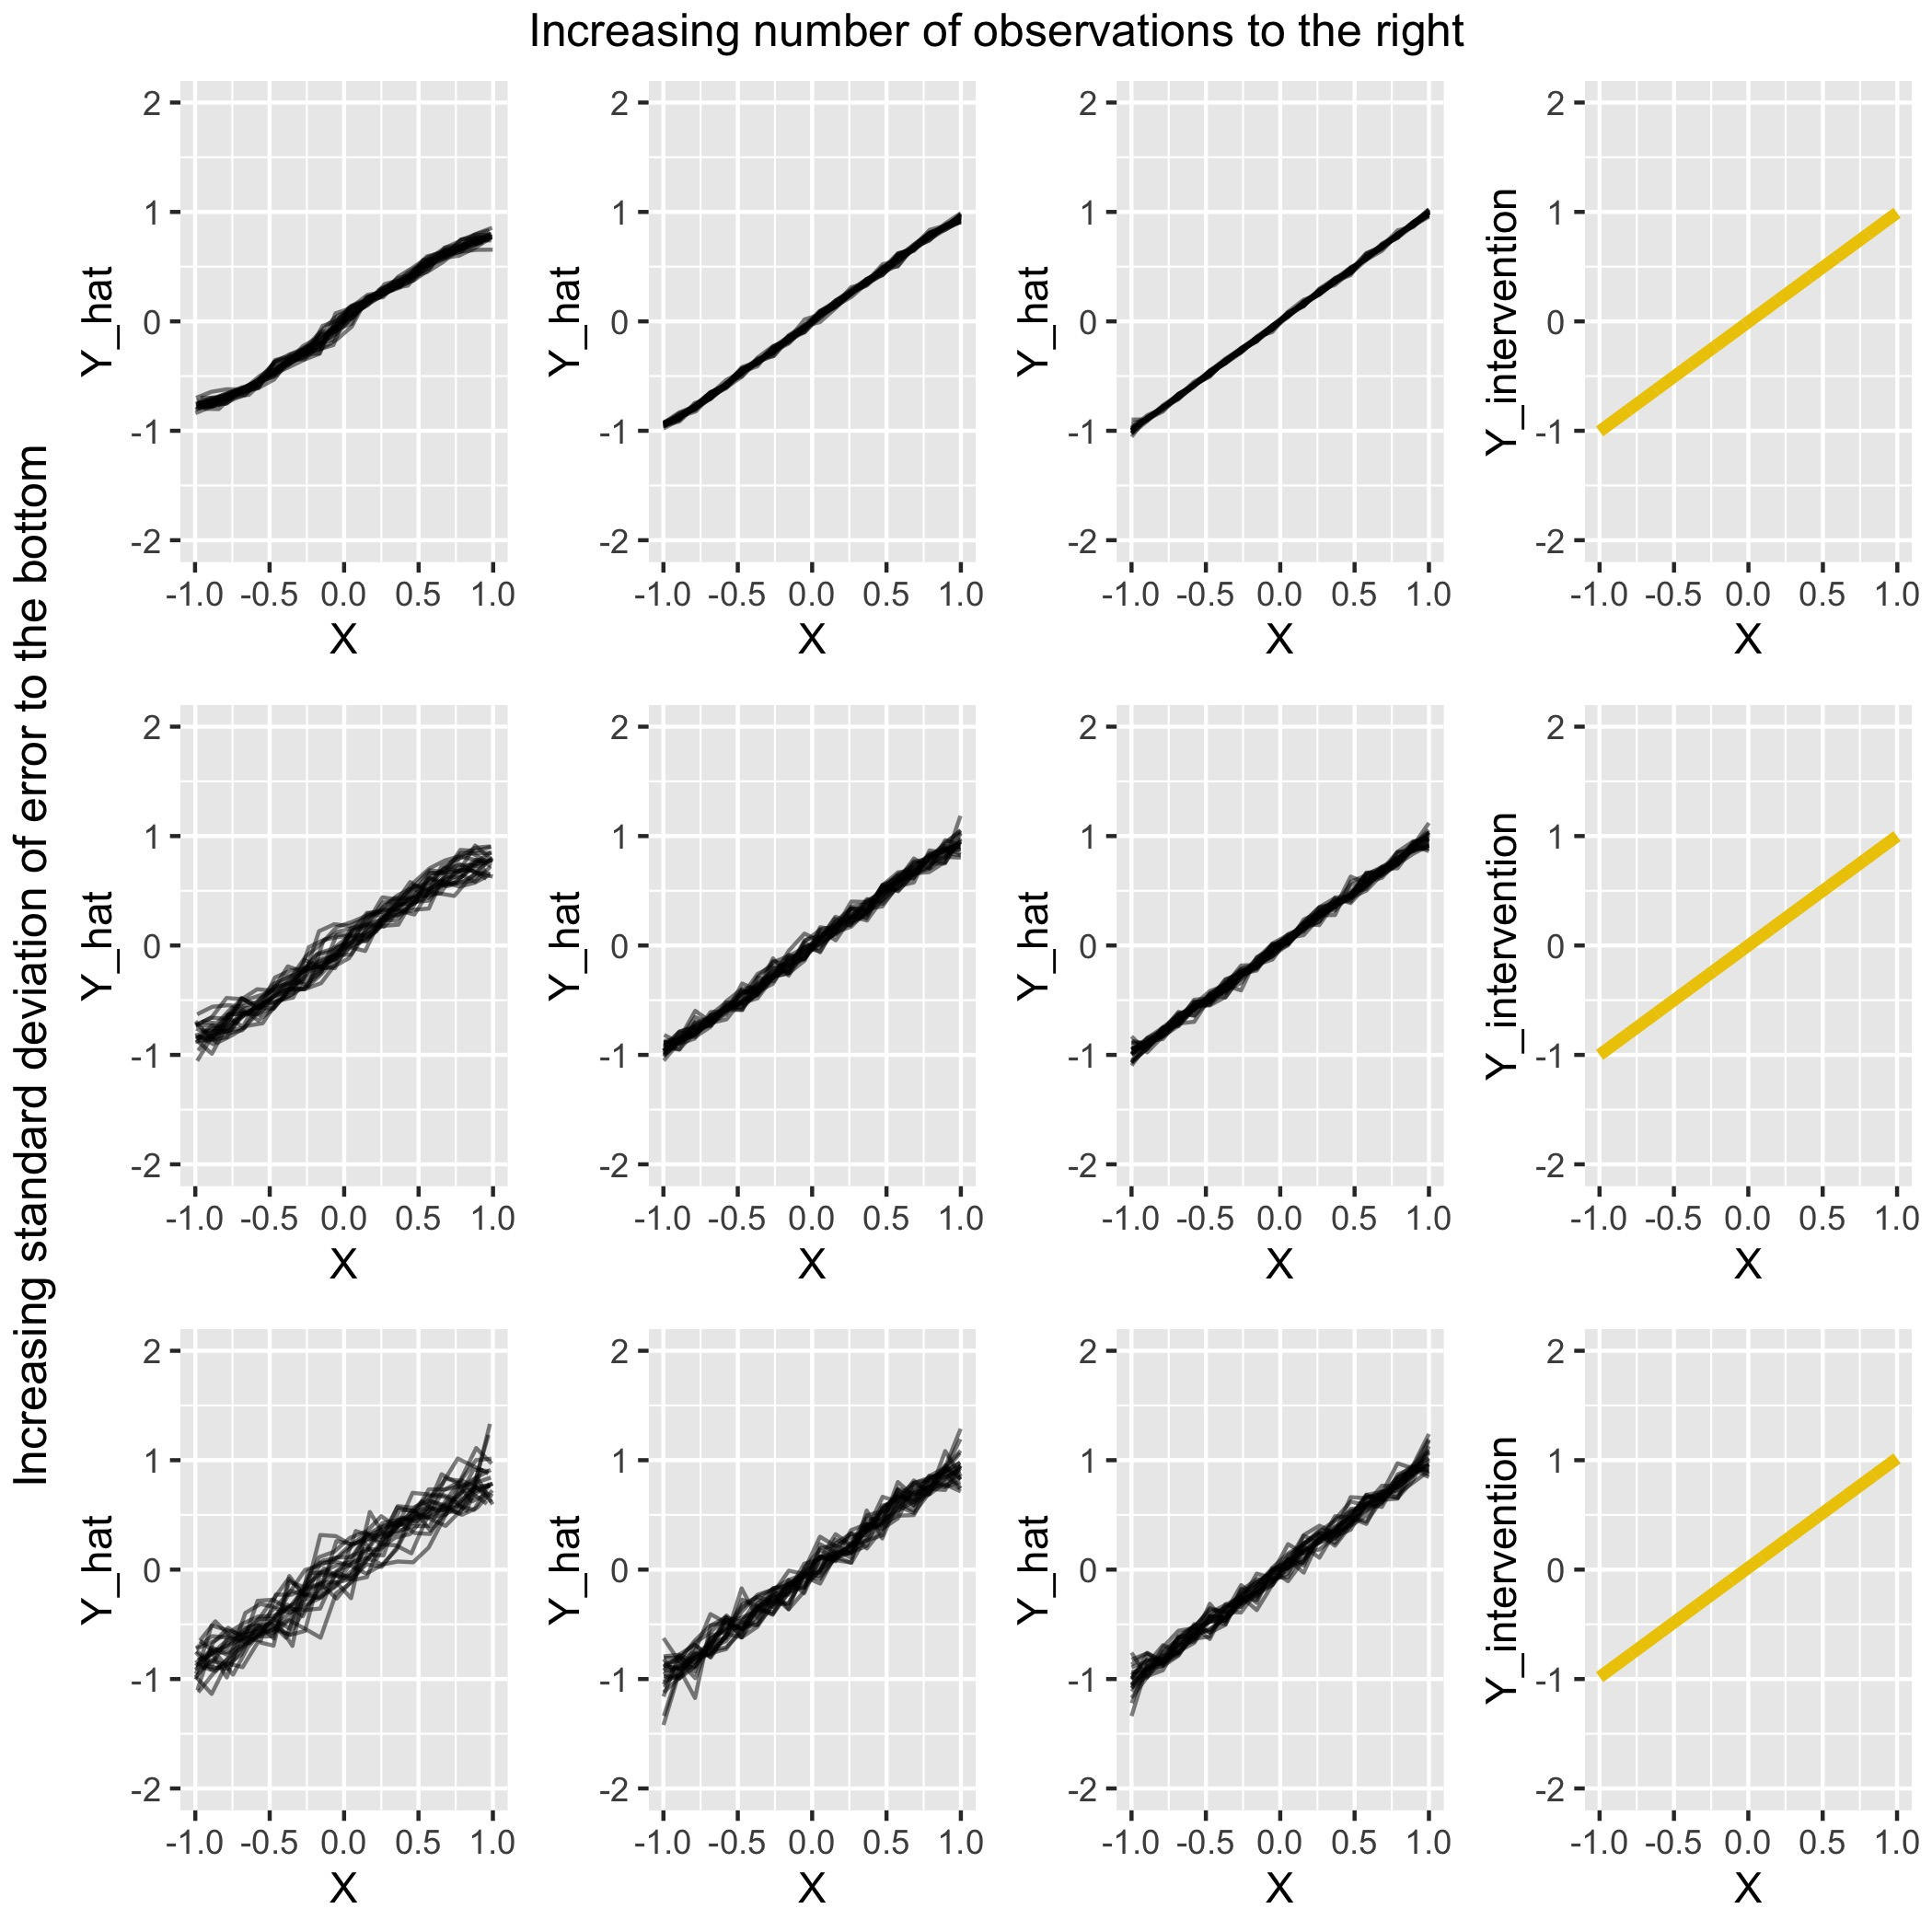
\includegraphics[width=1\linewidth]{images/scenario4_all} \hfill{}

\caption{Comparison for scenario 4 of PDPs under various settings with the (yellow) intervention curve on the right}\label{fig:Figure10causal}
\end{figure}

The PDPs in Figure \ref{fig:Figure10causal} are able to capture the
intervention curve well. Only in the cases where \(N=100\) is there
slight curvature at the extreme ends of \(X\). With this low number of
observations the model is less accurate. In all other settings a
consistent slope is present from \(X = -1\) to \(X = 1\), with the scale
of \(\hat{Y}\) matching that of \(Y_{intervention}\).

\textbf{Scenario 5}

In this scenario Z is a confounding variable. This is similar to
scenario 3 where \(X\) was the confounder. Thinking back to the example
of \emph{age} being a confounding variable for \emph{level of physical
activity} and \emph{weight gain}, in the previous example our \(X\) was
comparable to the confounder \emph{age}. In this scenario, we can keep
the same example, but say our variable \(X\) is now comparable to the
variable \emph{level of physical activity} that is being confounded.
Since \(X\) has no descendants and there is no backdoor path, the
expectation here is that the PDPs will be similar to the intervention
curve.

\begin{figure}
\centering
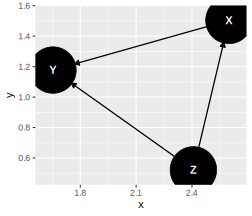
\includegraphics{book_files/figure-latex/Figure11causal-1.pdf}
\caption{\label{fig:Figure11causal}Z is a confounding variable impacting
both X and Y}
\end{figure}

The following simulation settings were used:

\[ Y \leftarrow Z + X + \epsilon_Y  \]
\[ \epsilon_Y,\epsilon_X ~ \sim \mathcal{N}(0, 0.1), \ \ \ \ \ \epsilon_Z \sim \mathcal{U}(-1,1), \ \ \ \ \ Z \leftarrow \epsilon_Z, \ \ \ \ \ X \leftarrow Z + \epsilon_X, \ \ \ \ \ N \leftarrow 100 \]

\begin{figure}

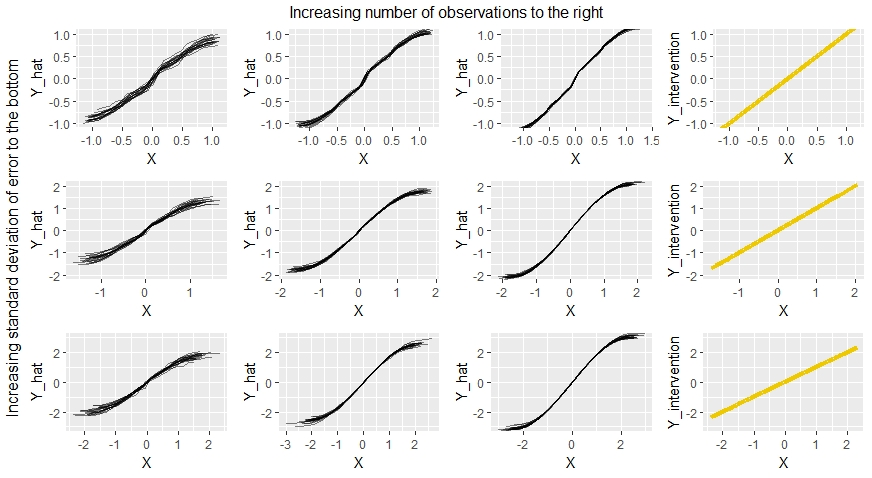
\includegraphics[width=1\linewidth]{images/scenario5_all} \hfill{}

\caption{Comparison for scenario 5 of PDPs under various settings with the (yellow) intervention curve on the right}\label{fig:Figure12causal}
\end{figure}

We can see in Figure \ref{fig:Figure12causal} that aside from the
extreme regions of \(X\) where the slope is flatter, the PDPs are fairly
similar to the Intervention Curves on the right. We can see that as the
standard deviations of the errors increase, so does the range of
\(Y_intervention\) from (-1, 1) to (-2,2). This same trend can be
observed in the PDPs. As could be expected, the PDPs with the highest
number of observations are are most accurate and have the lowest
standard deviation of errors.

\section{Conclusion}\label{conclusion}

Causal interpretability of a PDP is dependent on several things: (1) The
backdoor criterion being met. We have seen that if the backdoor
criterion is met, meaning no variable in the complement set \(C\) is a
descendant of our variable of interest, the PDP should be the same as
the intervention curve. We say should, because in practice it will also
depend on: (2) The model fit. Even when the backdoor criterion is met,
the PDP might not fully capture the exact same relationship as the
intervention curve. Especially in extreme regions, where data is
potentially sparse, the PDP can be deceptive. Same in scenarios with a
higher(er) error and low number of observations.

Point (2) can be estimated with the standard goodness of fit measures
that are pervasive in the statistics literature. It may be noted that
models may show a good fit, but do not learn the patterns that we would
expect them to learn from a theoretical point of view. Point (1) is even
more difficult to verify, especially based on only the data. Here a
certain amount of domain knowledge is needed to ensure the assumption is
met. Still, it is a hard assumption to verify which could limit the
confidence people have in a causal interpretation of a PDP. In the two
variable case we may already have difficulty finding a causal
interepretation. As we saw with the ice-cream example, the direction of
the dependency already makes a large difference. In many cases, the
necessary domain knowledge may be hard to attain.

\chapter{Introduction to Accumulated Local Effects (ALE)}\label{ale}

\emph{Authors: Jakob Bodensteiner, Nikolas Fritz}

\emph{Supervisor: Christian Scholbeck}

\section{Motivation}\label{motivation-1}

As seen in section 2 PDPs don't work well as soon as two or more
features are correlated. This gives rise to the definition of ALEs.
Although their definition makes sense for high dimensional feature
spaces including categorical features, within this section we only treat
a space with two continuous features.

\section{The Theoretical Formula}\label{ale-intro-formula}

The uncentered ALE with respect to a starting point \(z_{0, j}\) is
defined by \citep{Apley2016} as

\[  \widetilde{ALE}_{\hat{f},~j}(x) = \hat{f}_{x_j,ALE}(x) = \int_{z_{0,~j}}^{x} E_{X_c \mid X_j} [\hat{f}^j(X_j,~X_c)\mid X_j = z_j]~dz_j,\]
where \(\hat{f}\) is an arbitrary prediction function, as well as
\(\hat{f}^j(*,*)\) its j-th partial derivative. In this context \(X_j\)
is the feature of interest while \(X_c\) represents the other features.

\subsection{Centering}\label{centering}

The ALE (centered ALE) is defined as

\[  ALE_{\hat{f},~j}(x) = \widetilde{ALE}_{\hat{f},~j}(x) - E_{X_j}[\widetilde{ALE}_{\hat{f},~j}(X_j)]\]

The centering makes sense as it helps to interpret the ALE in a
reasonable way. This will be explained in section
\ref{ale-intro-interpret}.

\section{Estimation Formula}\label{estimation-formula}

Since this theoretical formula is of no use for a black box model with
unknown or even non-existing gradients, an approximative approach will
be used. The uncentered ALE can be approximated by the formula

\[ \widehat{\widetilde{ALE}}_{\hat{f},~j}(x) = \int_{z_{0,~j}}^{x} \sum_{k=1}^{K}    \frac{1_{I_k}(x_j)}{n_j(k)}\sum_{i:x_j^{(i)}\in N_j(k)} \frac{[\hat{f}(z_{k,~j}, x_{\setminus j}^{(i)})-\hat{f}(z_{k-1,~j}, x_{\setminus j}^{(i)})]}{z_{k,~j}-z_{k-1,~j}}~dx_j~.  \]

In a first step the relevant dimension of the feature space is divided
into K intervals beginning with the starting point \(z_{0, j}\). As it
is not clear how to exactly divide the feature space, section 3.x deals
with that question. The upper boundary of the k-th interval is denoted
by \(z_{k, ~j}\) as well as the lower boundary by \(z_{k-1, ~j}\). The
half-open interval \(]z_{k-1,~j},~z_{k,~j}]\) is defined as \(I_k\).
\(N_j(k)\) denotes the k-th interval, i.e. \(]z_{k-1,~j}, z_{k,~j}]\)
and \(n_j(k)\) the total number of observations having the j-value
within this interval. \(x_j^{(i)}\) is the j-value of the i-th
observation and correspondingly \(x_{\setminus j}^{(i)}\) the values of
the other features. The term on the right approximates the expected
partial derivative within each interval. Therefore each instance within
an interval is shifted to the upper and lower limit of the interval and
the total difference of the prediction is calculated. Divided by the
length of the interval this is a reasonable approximation for the
``local'' effect on the prediction, if the feature of interest changes
(cet. par.). By averaging these approximations over all observations
within the k-th interval, we receive a rough estimator for the term
\(E_{X_c \mid X_j} [\hat{f}^j(X_j,~X_c)\mid X_j \in N_j(k)]\), which we
take as constant effect for the k-th interval. By integrating over this
step function, which represents the locally estimated derivatives, the
(local) changes are accumulated. That's why the name Accumulated Local
Effects is quite reasonable. The approximative formula for the centered
ALE follows directly as

\[ \widehat{ALE}_{\hat{f},~j}(x) = \widehat{\widetilde{ALE}}_{\hat{f},~j}(x) - \frac{1}{n} \sum_{i=1}^{n} \widehat{\widetilde{ALE}}_{\hat{f},~j}(x_j^{(i)})~. 
 \]

\subsection{Implementation Formula}\label{implementation-formula}

As both the centered and the uncentered ALE estimations are piecewise
linear functions (integration over a step function), one can first
calculate the ALE at the interval boundaries and interpolate in a second
step. Therefore the following formula proposed by \citep[page
11]{Apley2016} with slightly changed notation will be useful. The
definitions of its components are as above. Additionally \(k_j(x)\) is
defined as the number of the interval that contains \(x\), i.e.
\(x \in ~]z_{k_j(x)-1,~j},~z_{k_j(x),~j}]\).

\[  \widehat{\widetilde{ALE}}_{steps,~\hat{f},~j}(x) =  \sum_{k=1}^{k_j(x)}   \frac{1}{n_j(k)}\sum_{i:~x_j^{(i)}\in N_j(k)} [\hat{f}(z_{k,~j}, x_{\setminus j}^{(i)})-\hat{f}(z_{k-1,~j},~x_{\setminus j}^{(i)})].  \]
This formula returns a step function. The values in each interval are
the accumulated values of the averaged total differences in each
interval. To transfer this formula into the correct estimator of the
uncentered ALE one has to linearely interpolate the points
\((z_{k-1,~j},~\widehat{\widetilde{ALE}}_{steps,~\hat{f},~j}(z_{k-1,~j}))\)
with
\(( z_{k,~j},\widehat{\widetilde{ALE}}_{steps,~ \hat{f},~j}(z_{k,~j}))\)
for \(k \in \{1, ..., K \}\) and
\(\widehat{\widetilde{ALE}}_{steps, \hat{f},j}(z_{0,~j}) = 0\).

Since in this formula there is no integral, it is easier to implement.

\section{Intuition and Interpretation}\label{ale-intro-interpret}

As the former sections introduced the theoretical basics for the ALE,
this section shall provide an intuition as well for the calculation
method as for the interpretation. As described above, the local
behaviour of the model with respect to the variable of interest is
estimated by moving the existing data points to the boundaries of their
interval and evaluating the total difference of the prediction for the
``new'' data points. Figure \ref{fig:dataALE} first offered by
\citep{molnar2019} gives a good intuition for this procedure.

\begin{figure}
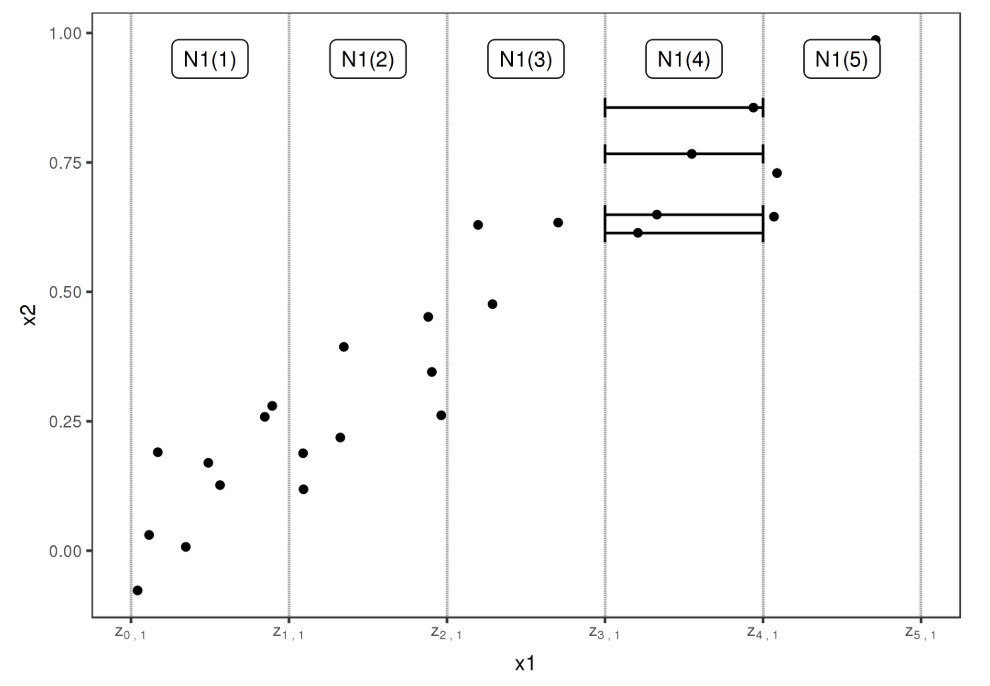
\includegraphics[width=1\linewidth]{images/ale_estimation_intuition} \caption{The data points within the 4-th interval are shifted
to the interval boundaries \(z_{3,~1}\) and \(z_{4,~1}\).}\label{fig:dataALE}
\end{figure}




First one splits the total range of the variable of interest (in this
case \(x_1\)) to intervals of suitable size.\\
For each interval the contained data points are moved to the interval
boundaries. One gets twice as much ``simulated'' new data points as
originally contained in each interval. The prediction function is now
evaluated at these simulated points and the total difference of the
prediction (for the given interval) is estimated as the mean change.
Divided by the length of the interval one gets an estimation for the
partial derivative within this interval. Theoretically one receives the
uncentered ALE by integration over this step function. Technically in a
first step the total change per interval is accumulated. In a second
step linear interpolation at the interval boundaries simulates a
constant change within each interval. Both variants lead to the same
result.

As the evaluation is ideally done on relatively small intervals, on the
one hand the local behaviour of the model is estimated. On the other
hand the covariance structure of the features is taken into account, as
only ``realistic'' data points are simulated. This is in accordance with
sampling from the conditional distribution.

In a last step the uncentered ALE is centered, i.e.~shifted by a
constant such that the expectation of the centered ALE is zero.

Figure \ref{fig:aleEx} shows an example ALE which could match the data
situtaion of Figure \ref{fig:dataALE}.

\begin{figure}
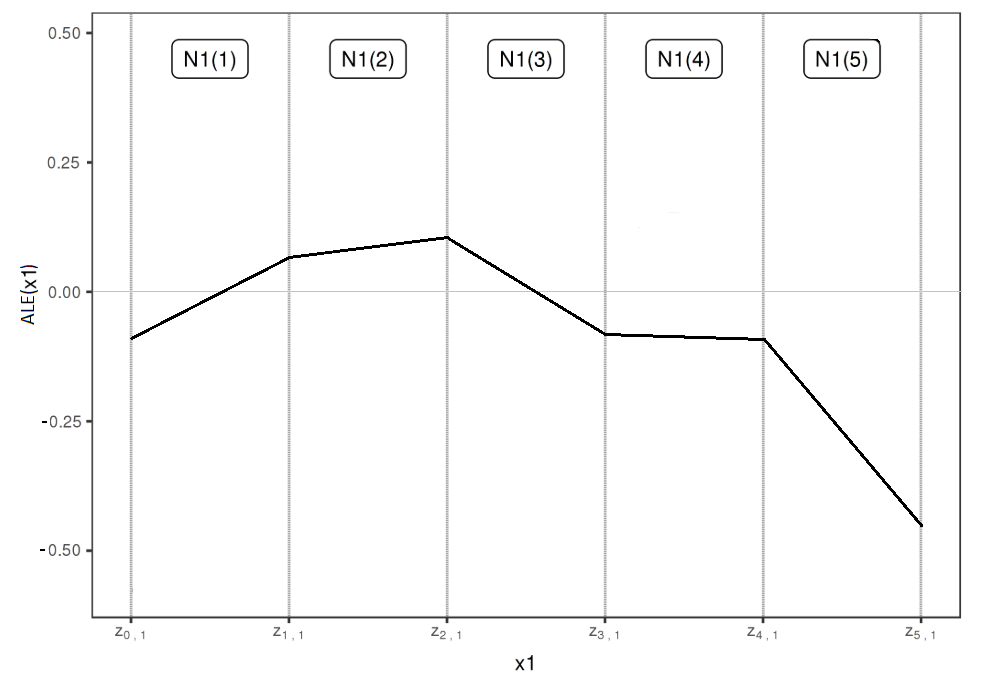
\includegraphics[width=1\linewidth]{images/ale_example} \caption{ALE on basis of 5 intervals}\label{fig:aleEx}
\end{figure}



To understand the interpretation of the ALE it can be useful to first
have a look at the intuition behind the uncentered ALE. If the value of
the uncentered ALE at \(x_1 = 2\) equals \(1\), this means that if one
samples a data point from the joint distribution of both features but
only knows that \(x_1 = 2\), one would expect the prediction to be 1
higher than the average prediction for realistic data points at
\(x_1 = z_{0,1}\) (i.e.~data points sampled from the conditional
distribution at \(x_1 = z_{0,1}\)). This expectation strongly depends on
the reference point \(z_{0,1}\), which per definition is smaller than
the smallest \(x_1\)-value of the data. By substracting the expectation
of the uncentered ALE - which is the mean difference of the prediction
of a data point from the joint distribution to the prediction of a
realistic data point(i.e.~from the conditional distribution) at
\(x_1 = z_{0,1}\) - the interpretation becomes a lot easier. If the
value of the (centered) ALE at \(x_1 = 2\) equals for example \(2\),
this means that, if one samples a data point from the joint distribution
of both features and \(x_1\) equals 2, one would expect the 1st order
effect of feature \(x_1\) to be 2 higher than the average 1st order
effect of this feature.

So far only the case of 2-dimensional feature spaces with one feature of
interest was taken into account. In the following chapters methods and
interpretation for ALE with two numeric features (second order effects)
or one categorical feature will be in the focus. Furthermore we will
have a look on the size of the intervals the data is evaluated on, which
can be crucial for the expressiveness of the ALE.

\chapter{Comparison of ALE and PDP}\label{ale-pdp}

\emph{Author: Jakob Bodensteiner}

\emph{Supervisor: Christian Scholbeck}

This subchapter of ALE will focus on the comparison of ALE and PDP,
especially on the influence of correlation in the underlying datasets.
At first, the interpretation for the regular one dimensional (or 1D) ALE
to the 1D PDP will be discussed. Thereafter two-dimensional ALEs will be
introduced and their difference to PDPs will be explained. Additionally,
a runtime comparison will be shown and to conclude this chapter a
real-world example will be analyzed with ALE, PDP and ICE plots.

\section{Comparison one feature}\label{comparison-one-feature}

So far in this book, one could already see a few examples of the PDP for
one feature and its limitations. The ALE is kind of the solution for the
biggest issue with the PDP. The ALE can interpret models predicting on
correlated variables correctly, while the PDP may fail in this case.
Before the two methods will be compared, here comes a short reminder
regarding the interpretation.

Given a value for the feature of interest \ldots{}

\ldots{}the 1D PDP measures the expected prediction for this value by
averaging over the prediction of all observations pretending the feature
of interest is that value.

\ldots{} the 1D ALE shows the expected and centered first order effect
of this feature.

With these interpretations in mind, the first example with artificial
data will be discussed.

\subsection{Example 1: Multiplicative prediction
function}\label{example-1-multiplicative-prediction-function}

The following Problem is constructed: There is a data set consisting of
150 observations with three features (\(x_1\), \(x_2\), \(x_3\)) and the
target variable \(y = x_1 x_2 x_3\). The features of each observation
are sampled from the following disrtibutions:
\(X_1 \sim \mathcal{U}(0,~0.5)\), \(X_2 \sim \mathcal{N}(2,~2)\) and
\(X_3\mid X_2, X_1 \sim \mathcal{N}(X_2,X_1)\).

So features one and two are independent of each other, while \(x_3\) is
strongly correlated with \(x_2\). It is also not independent from
\(x_1\), although there is no influence of \(x_1\) on the expected value
of \(x_3\).

In this example (and in all other examples with artificial data in this
chapter) the prediction function is not fitted but sets as the target
variable, here \(f(x_1, x_2, x_3) = y = x_1 x_2 x_3\). By setting the
prediction function instead of fitting a learner on the data it is
ensured that one can imagine how the `real' influence of each feature
would look like. This way one can see clearly if ALE or PDP are making
mistakes in the interpretation. If one would fit a random forest one
could never be sure if the ALE and PDP plots are making a mistake in
explaining the fitted model or if the mistake is made by the learner and
the explanation of the learner itself would be fine. This will become
clear at the end of the chapter when the real-world example will be
discussed.

\begin{figure}
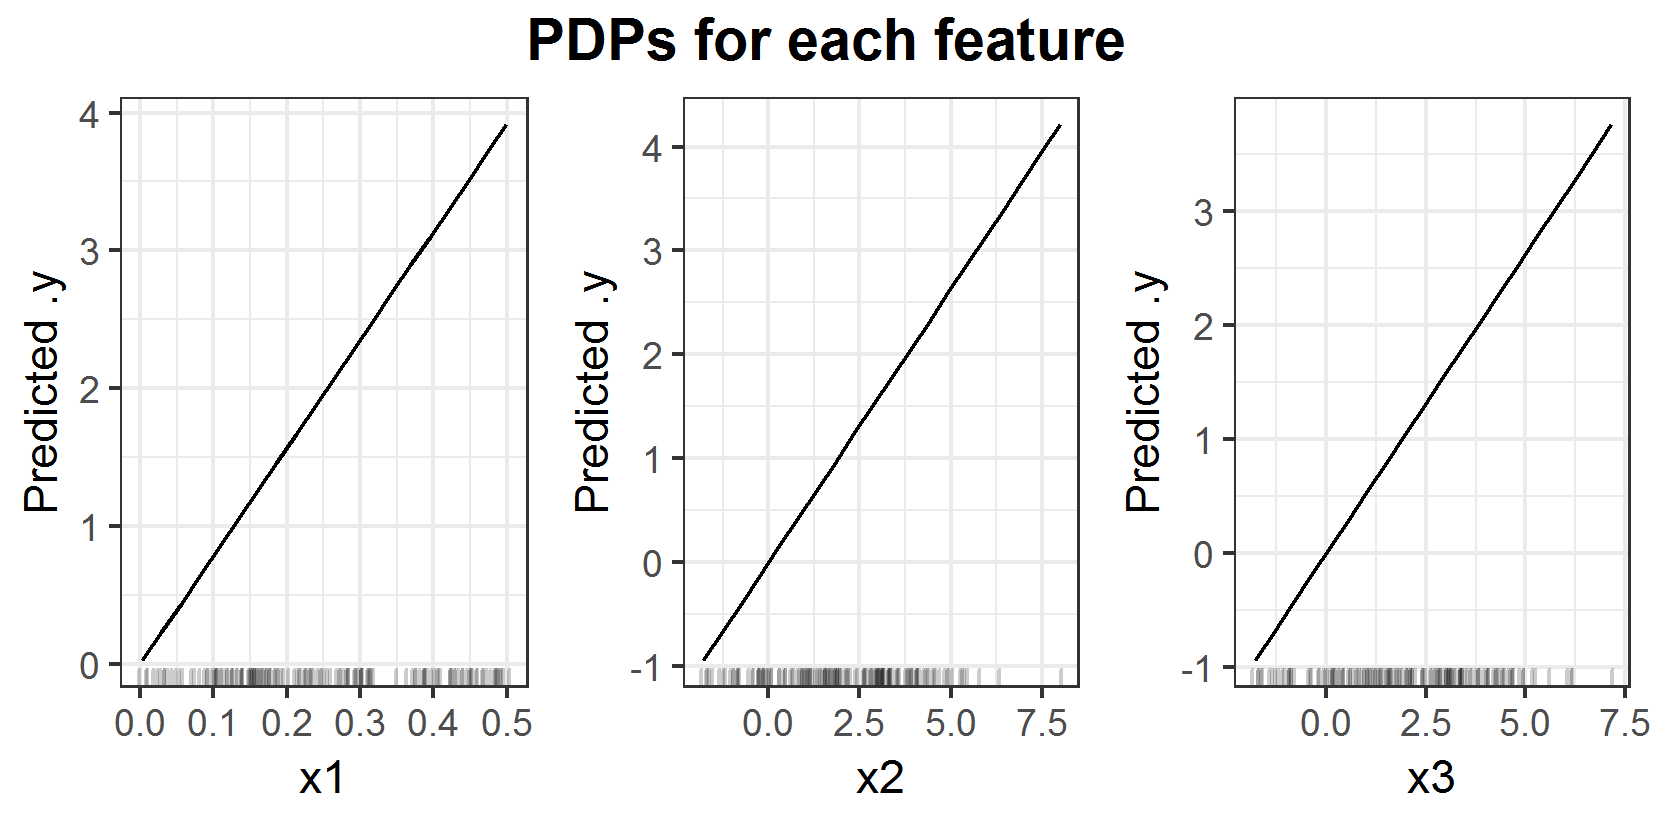
\includegraphics[width=1\linewidth]{images/ale_1_PDPs_x1x2x3_150_0_0p5_2_2} \caption{PDPs for prediction function
\(f(x_1, x_2, x_3) = x_1 x_2 x_3\).}\label{fig:pdpsx1x2x3}
\end{figure}




\begin{figure}
\includegraphics[width=1\linewidth]{images/ale_1_ALEs_x1x2x3_150_0_0p5_2_2} \caption{ALEs for prediction function
\(f(x_1, x_2, x_3) = x_1 x_2 x_3\).}\label{fig:alesx1x2x3}
\end{figure}




Plot \ref{fig:pdpsx1x2x3} shows the 1D PDP for each of the three
features. One can see that the PDP detects a linear influence on the
prediction for all 3 of the features.

On the other hand, the ALE (figure \ref{fig:alesx1x2x3}) attests the
linear influence to the feature \(x_1\) only. This plot exposes a
weakness of the ALE compared to the PDP straight away. The ALE depends
much more on the sampled data than the PDP does. The result is that the
ALE can look a bit shaky. In this special case, it is that seriously one
almost can't see the linear influence. If there would be more data or
fewer intervals for the estimation, the plot would look more like the
PDP for feature \(x_1\). The two other features seem to rather have a
quadratic influence on the prediction. And this is the case indeed since
it is the `true' link between prediction and the correlated features.
Feature \(x_3\) has (in expectation) the same value as \(x_2\).
Especially if feature \(x_1\) has small values the variance of feature
\(x_2\) around \(x_3\) becomes small as well. As consequence the last
part of the prediction function `\(x_2 x_3\)' can be approximated by
`\(x_2^2\)' or `\(x_3^2\)'. This explains the quadratic influence. By
changing the prediction formula to \(f(x_1, x_2, x_3) = y = x_1 x_2^2\)
the figures \ref{fig:pdpsx1x22} and \ref{fig:alesx1x22} for PDP and ALE
plots are estimated.

\begin{figure}
\includegraphics[width=1\linewidth]{images/ale_1_PDPs_x1x22_150_0_0p5_2_2} \caption{PDPs for prediction function
\(f(x_1, x_2, x_3) = x_1 x_2^2\).}\label{fig:pdpsx1x22}
\end{figure}




\begin{figure}
\includegraphics[width=1\linewidth]{images/ale_1_ALEs_x1x22_150_0_0p5_2_2} \caption{ALEs for prediction function
\(f(x_1, x_2, x_3) = x_1 x_2^2\).}\label{fig:alesx1x22}
\end{figure}




Plots \ref{fig:pdpsx1x22} and \ref{fig:alesx1x22} clearly show the
linear influence of \(x_1\) again. Additionally this time both (ALE and
PDP) attest a quadratic influence to feature \(x_2\) on the prediction.
Since \(x_3\) does not have any influence on the prediction function, it
is correct, that there is no influence detected. The reason for this
behavior lies in the calculation method for the PDP. With the new
prediction formula only depending on uncorrelated features \(x_1\) and
\(x_2\), the PDP works well. Since now the approach of PDP to calculate
the mean effect is correct.

\subsection{Example 2: Additive prediction
function}\label{example-2-additive-prediction-function}

In this example, PDP and ALE will be applied to an additive prediction
function.

A data set consisting of three features (\(x_1\), \(x_2\), \(x_3\)) is
constructed. In this case the target variable is
\(y = x_1 + x_2 - x_3\). Once again the prediction function is not
learned but set to exactly the target variable, meaning
\(f(x_1, x_2, x_3) = x_1 + x_2 - x_3\). The distributions are similar to
the ones from example 1 and again 150 observations are sampled.
\(X_1 \sim \mathcal{U}(0,~2)\), \(X_2 \sim \mathcal{N}(2,~0.5)\) and
\(X_3\mid X_2 \sim \mathcal{N}(X_2,~0.5)\)

\begin{figure}
\includegraphics[width=1\linewidth]{images/ale_1_PDPs_x1_plus_x2_minus_x3_150_0_2_0p5} \caption{PDPs for prediction function
\(f(x_1, x_2, x_3) = x_1 + x_2 - x_3\).}\label{fig:pdpsx1px2mx3}
\end{figure}




\begin{figure}
\includegraphics[width=1\linewidth]{images/ale_1_ALEs_x1_plus_x2_minus_x3_150_0_2_0p5} \caption{ALEs for prediction function
\(f(x_1, x_2, x_3) = x_1 + x_2 - x_3\).}\label{fig:alesx1px2mx3}
\end{figure}




For this example one can see that the ALEs (\ref{fig:alesx1px2mx3}) and
PDPs (\ref{fig:pdpsx1px2mx3}) are basically the same. Ignoring the
centering both attest the same linear influence for all three features.
And since it is an additive model this is actually correct. But neither
the ALE nor the PDP recognize the strong correlation between the
features \(x_2\) and \(x_3\). The real influence of features \(x_2\) and
\(x_3\) is in expectation zero, since it is \(x_2 - x_3\) and
\(E[X_3 \mid X_2] = X_2\). So \(E[X_2 - X_3 \mid X_2] = 0\).

This shows a few points one has to be aware of when working with these
plots. In this example, if one uses the interpretation of the PDP for
feature \(x_2\) and states `If the value of feature \(x_2\) is 2.5, then
I expect the prediction to be 1.5' it would be wrong. The problem here
is the extrapolation in the estimation of the PDP. So it does not take
into account any connection between the features but still works as good
as the ALE in this example.

The general advantage of the ALE is the small chance of extrapolation in
the estimation. But this does not mean it would recognize any
correlation between the features in each scenario. And it is in general
not possible to state something about the prediction with only one 1D
ALE. The ALE is just showing the expected and centered main effect of
the feature. In this example an interpretation like `If feature \(x_2\)
has value 2.5 then in expectation the prediction will be 0.5 higher than
the average prediction' is wrong. If one needs a statement like that the
other strongly correlated features have to be taken into account as
well. One has to be aware of the higher order effects of the ALE, too.

To conclude the analysis of this example 2D ALEs are necessary. So it
will be continued later this chapter.

\section{Comparison two features}\label{comparison-two-features}

Before the 2D ALE and PDP will be applied to the same predictors, the 2D
ALE has to be introduced. In the first place, the theoretical formula
will be defined. Thereafter the estimation will be derived and then the
comparison to the 2D PDP will be made.

\subsection{The 2D ALE}\label{the-2d-ale}

\subsubsection{Theoretical Formula 2D
ALE}\label{theoretical-formula-2d-ale}

Similar to one variable of interest there is a theoretical formula for a
2-dimensional ALE. This ALE aims to visualize the 2nd order effect.
Meaning one will just see the additional effect of interaction between
those two features. The main effects of the features will not be shown
in the 2D ALE.

To explain the formula it will be assumed that \(x_j\) and \(x_l\) are
the two features of interest. The rest of the features is represented by
\(x_c\). So in the following variable \(x_c\) can be of higher dimension
than 1. As for the 1D ALE, there is again a theoretical derivative for
the fitted function \(\hat{f}\). But this time it is the derivative in
the direction of both features of interest. So in the following, this
notation will hold:

\[ \hat{f}^{(j,~l)}(x_j,~x_l,~x_c) = \frac{\delta\hat{f}(x_j,~x_l,~x_c)}{\delta x_j~ \delta x_l}\]

The whole formula would be very long, so it is split into 3 parts
(compare \citep[page 8]{Apley2016}):

\begin{enumerate}
\def\labelenumi{\arabic{enumi}.}
\item
  The 2nd order effect \eqref{eq:ale2DTheoretical1stLvl}
\item
  2nd order effect corrected for both main effects
  \eqref{eq:ale2DTheoreticalCorrection}
\item
  The 2D ALE; the corrected 2D ALE centered for its mean overall effect
  \eqref{eq:ale2DTheoretical}
\end{enumerate}

Equation \eqref{eq:ale2DTheoretical1stLvl} is the 2nd order effect with no
correction for main effects of \(x_j\) and \(x_l\). So this is not yet
the pure 2nd order effect the 2D ALE is aiming for.

\begin{equation} 
\widetilde{\widetilde{ALE}}_{\hat{f},~j,~l}(x_j, x_l) = \notag
\end{equation}

\begin{equation}
\int_{z_{0,j}}^{x_j}  \int_{z_{0,l}}^{x_l} E[\hat{f}^{(j,~l)}(X_j,~X_l,~X_c)\mid X_j = z_j,~X_l = z_l]~dz_l~dz_j 
  \label{eq:ale2DTheoretical1stLvl}
\end{equation}

Now from the uncorrected 2nd order effect, the two main effects of both
features on the uncorrected 2D ALE are subtracted (see equation
\eqref{eq:ale2DTheoreticalCorrection}). In this way the main effects of
\(x_j\) and \(x_l\) on the final \(ALE_{\hat{f},~j,~l}(x_j, x_l)\) are
both zero \citep[page 9]{Apley2016}. But be careful, this is not
centering by a constant as in the one-dimensional ALE. This is a
correction for the also accumulated main effects which of course vary in
the directions of the features.

\begin{align}
\widetilde{ALE}_{\hat{f},~j,~l}(x_j, x_l) 
= &\widetilde{\widetilde{ALE}}_{\hat{f},~j,~l}(x_j, x_l) \notag \\ 
&-  \int_{z_{0,~j}}^{x_j}  E[\frac{\delta\widetilde{\widetilde{ALE}}_{\hat{f},~j,~l}(X_j, X_l)}{\delta X_j}\mid X_j = z_j]~dz_j \notag \\
&- \int_{z_{0,~l}}^{x_l}  E[\frac{\delta\widetilde{\widetilde{ALE}}_{\hat{f},~j,~l}(X_j, X_l)}{\delta X_l}\mid X_l = z_l]~dz_l
\label{eq:ale2DTheoreticalCorrection}
\end{align}

Equation \eqref{eq:ale2DTheoretical} shows the final (centered) 2D ALE.
The subtraction in the formula is now the real centering to shift the
2nd order effect (corrected for the main effects) to zero with respect
to the marginal distribution of \((X_j, ~ X_l)\).

\begin{equation} 
ALE_{\hat{f},~j,~l}(x_j, x_l) = \widetilde{ALE}_{\hat{f},~j,~l}(x_j, x_l) ~ -  E[\widetilde{ALE}_{\hat{f},~j,~l}(X_j, X_l)]
  \label{eq:ale2DTheoretical}
\end{equation}

In the appendix \ref{ale-2d-example-calculation} one can find the
calculation of the theoretical ALE for Example 1.

\subsubsection{Estimation 2D ALE}\label{estimation-2d-ale}

Analogously to the 1D ALE in most cases, it is not possible to calculate
the 2D ALE. It has to be estimated. These estimation formulas are pretty
long and might be confusing, especially the indices. But there will be
an explanation including a visualization as well to clarify the
estimation method.

First, all variables have to be defined. The two features of interest
are \(x_j\) and \(x_l\). The prediction function is
\(\hat{f}(x_j, x_l, x_{\setminus\{j,~l\}})\), while
\(x_{\setminus\{j,~l\}}\) represents all the rest of the features, so it
can be of higher dimension than 1. The areas including data for feature
\(x_j\) and \(x_l\) are divided into the same number of intervals,
namely K. The intervals in \(x_j\) direction are separated by
\(z_{k,j}\) for \(k \in \{0,...,K\}\). \(k_j(x_j)\) returns the interval
number in which \(x_j\) lies. This holds for \(z_{m,l}\) and
\(k_l(x_l)\) respectively in direction of \(x_l\). \(N_{\{j,~l\}}(k,m)\)
is the crossproduct of the k-th and m-th interval (in \(x_j\) and
\(x_l\) direction), so it is defined as
\((z_{k-1,j}, z_{k,j}] \times (z_{m-1,j}, z_{m,j}]\).
\(n_{\{j,~l\}}(k,m)\) is the number of observations lying in this
\(N_{\{j,~l\}}(k,m)\) cell. The parameter i represents the i-th
observation \citep{Apley2016}. With these variables in mind, the
definition of the 2D ALE estimation can begin.

The estimation equvalent to Formula \eqref{eq:ale2DTheoretical1stLvl} is:

\begin{equation} 
\widehat{\widetilde{\widetilde{ALE}}}_{\hat{f},~j,~l}(x_j, ~x_l) = \notag
\end{equation}

\begin{equation}
\sum_{k=1}^{k_j(x_j)} \sum_{m=1}^{k_l(x_l)}   \frac{1}{n_{\{j,~l\}}(k,m)}\sum_{i:~x_{\{j,~l\}}^{(i)}\in N_{\{j,~l\}}(k,m)} ~ \Delta_{\hat f}^{{\{j,~l\}}, ~k,~m} (x_{\setminus\{j,~l\}}^{(i)}),
  \label{eq:ale2DEst1stLvl}
\end{equation}

while the \(\Delta\) function is:

\begin{equation}
\Delta_{\hat f}^{{\{j,~l\}}, ~k,~m} (x_{\setminus\{j,~l\}}^{(i)}) = \notag
\end{equation}

\begin{equation}
[\hat f(z_{k,~j},~ z_{m,~l}, ~x_{\setminus\{j,~l\}}^{(i)}) - \hat f(z_{k-1,~j},~ z_{m,~l}, ~x_{\setminus\{j,~l\}}^{(i)})] \notag
\end{equation}

\begin{equation}
- [\hat f(z_{k,~j},~ z_{m-1,~l}, ~x_{\setminus\{j,~l\}}^{(i)}) - \hat f(z_{k-1,~j},~ z_{m-1,~l}, ~x_{\setminus\{j,~l\}}^{(i)})]
\label{eq:ale2DEstDelta} 
\end{equation}

Now the correction for the main effects (equation
\eqref{eq:ale2DEstCorrection} corresponding to theoretical formula
\eqref{eq:ale2DTheoreticalCorrection}) is estimated:

\begin{align}
\widehat{\widetilde{ALE}}_{\hat{f},~j,~l}(x_j, ~x_l) = 
&\widehat{\widetilde{\widetilde{ALE}}}_{\hat{f},~j,~l}(x_j, ~x_l) \notag \\
&-  \sum_{k=1}^{k_j(x_j)} \frac{1}{n_j(k)} \sum_{m=1}^{K} ~ n_{\{j,~l\}}(k,m) [\widehat{\widetilde{\widetilde{ALE}}}_{\hat{f},~j,~l}(z_{k,~j}, ~z_{m,~l}) \notag \\
&~~~~~~~~~~~~~~~~~~~~~~~
- \widehat{\widetilde{\widetilde{ALE}}}_{\hat{f},~j,~l}(z_{k-1,~j}, ~z_{m,~l})]\notag \\
&- \sum_{k=1}^{k_l(x_l)} \frac{1}{n_l(k)} \sum_{m=1}^{K} ~ n_{\{j,~l\}}(k,m) [\widehat{\widetilde{\widetilde{ALE}}}_{\hat{f},~j,~l}(z_{k,~j}, ~z_{m,~l}) \notag \\
&~~~~~~~~~~~~~~~~~~~~~~~ 
- \widehat{\widetilde{\widetilde{ALE}}}_{\hat{f},~j,~l}(z_{k,~j}, ~z_{m-1,~l})]
\label{eq:ale2DEstCorrection}
\end{align}

Equation \eqref{eq:ale2DEstCorrection} is the uncentered 2D ALE since it
is just corrected for its main effects. And this is not a real centering
in the sense of subtracting a constant value. Now it will be centered
for its estimation
\(E[\widehat{\widetilde{ALE}}_{\hat{f},~j,~l}(X_j, ~X_l)]\) and this is
a constant, so there will be no effect on the general shape of the ALE
plot. Again this expected value has to be estimated, to complete the 2D
ALE as is calculated in theoretical formula \eqref{eq:ale2DTheoretical}.

\begin{equation}  
\widehat{ALE}_{\hat{f},~j,~l}(x_j, ~x_l) = \notag
\end{equation}

\begin{equation}
\widehat{\widetilde{ALE}}_{\hat{f},~j,~l}(x_j, ~x_l) -
\sum_{k=1}^{K}\sum_{m=1}^{K} ~ n_{\{j,~l\}}(k,m) ~ \widehat{\widetilde{ALE}}_{\hat{f},~j,~l}(z_{k,~j}, ~z_{m,~l}) 
 \label{eq:ale2DEst}
\end{equation}

In contrast to the ALE for one feature of interest, the 2D ALE
(\eqref{eq:ale2DEst} is a two-dimensional step function, so there is no
smoothing or something similar to make it a continuous function.

These formulas are pretty long, so to get an intuition of the estimation
figure \ref{fig:ale2DEstimation} will be helpful.

\begin{figure}
\includegraphics[width=1\linewidth]{images/ale_1_ALE_2D_estimation} \caption{Visualization of the absolut differences for
the 2nd order effect \citep[page 13]{Apley2016} and \citep{molnar2019}.}\label{fig:ale2DEstimation}
\end{figure}




To calculate the delta \eqref{eq:ale2DEstDelta} for the uncorrected and
uncentered ALE estimation in each cell the predictions for the data
points in that cell will be calculated pretending the \(x_l\) and
\(x_j\) values are the corner values of the cell they are in. In the
case of figure \ref{fig:ale2DEstimation}, these 2-dimensional corner
values would be a, b, c, d. The delta for point x in this example would
be calculated like this:

\begin{align}
\Delta_{\hat f}^{{\{j,~l\}}, ~4,~3} (x_{\setminus\{j,~l\}}) = 
& [\hat f(b, ~x_{\setminus\{j,~l\}}) - \hat f(a, ~x_{\setminus\{j,~l\}})] \notag \\
&- [\hat f(d, ~x_{\setminus\{j,~l\}}) - \hat f(c, ~x_{\setminus\{j,~l\}})] \notag
\end{align}

The same would be done for point y. Thereafter the deltas would be
averaged to get the mean delta for cell \(N_{\{j,~l\}}(4,3)\). This
would then be accumulated over all cells left or beneath this cell to
get the uncorrected and uncentered ALE for the values in
\(N_{\{j,~l\}}(4,3)\).

The correction for the main effects extracts the pure 2nd order effect
for the two features of interest by subtracting the main effect of the
single features on the ALE (equation \eqref{eq:ale2DEstCorrection}). To
stick with this example the correction for the main effect of feature
\(x_j\) for values in \(N_j(4)\) takes into account all cells in the
first 4 columns and aggregates the first order effect. In cell
\(N_{\{j,~l\}}(4,3)\) this would look like this:

\[ \widehat{\widetilde{\widetilde{ALE}}}_{\hat{f},~j,~l}(b) - \widehat{\widetilde{\widetilde{ALE}}}_{\hat{f},~j,~l}(a)\]

The correction for \(x_l\) looks pretty much the same just from the
other direction. It takes into account the first 3 rows. So in cell
\(N_{\{j,~l\}}(4,3)\) the first order effect in direction of \(x_l\)
would be

\[ \widehat{\widetilde{\widetilde{ALE}}}_{\hat{f},~j,~l}(b) - \widehat{\widetilde{\widetilde{ALE}}}_{\hat{f},~j,~l}(d). \]

Thereafter the corrected ALE is centered for its mean (equation
\eqref{eq:ale2DEst}), pretty much the same way as is done for one
dimension. But this time the aggregation is not just over a line but
over a grid.

There are a few questions that might arise.

First, how is the grid for the estimation defined? In the iml package,
the cells are the cross products of the intervals used for the 1D
estimation. It would be very hard to make a grid of rectangles which all
include roughly the same amount of data points.

Another question is: How does the estimation treat empty cells, which
include no data points? There are two options, they can either be
ignored and greyed out or they receive the value of their nearest
neighbor rectangle, which is determined using the center of the cells.
The last method is implemented in the iml package. This happens right
after averaging over the
\(\Delta_{\hat f}^{{\{j,~l\}}, ~k,~m} (x_{\setminus\{j,~l\}})\)s before
the correction for the 1st order effects is done.

\subsubsection{Example 1 continued - Theoretical and estimated 2D
ALE}\label{example-1-continued---theoretical-and-estimated-2d-ale}

Before ALE and PDP will be compared for two features of interest, the
analysis of example 1 will be continued in two dimensions, to get a
first glance at the 2D ALE.

The data set is basically the same, just for sake of clearness in the 2D
ALE example the distributions are a bit different. A data set consisting
of 150 observations with three features (\(x_1\), \(x_2\), \(x_3\)) and
the prediction function \(f(x_1, x_2, x_3) = x_1 x_2 x_3\) is
considered. But this time the three features are sampled from these
disrtibutions: \(X_1 \sim \mathcal{U}(0,~0.5)\),
\(X_2 \sim \mathcal{N}(5,~1)\) and
\(X_3\mid X_2, X_1 \sim \mathcal{N}(X_2,X_1)\). So feature \(x_2\) is
expected to be 5 and has a lower variance than it has in example 1. The
rest stays the same.

With the formulas in the appendix \ref{ale-2d-example-calculation} it is
possible to calculate the theoretical 2D ALE.

\begin{figure}
\includegraphics[width=1\linewidth]{images/ale_1_ALE_2D_theo_vs_estim_x1x2x3_150_0_0p5_5_1} \caption{Theoretical 2D ALE (left) and estimated ALE (right).}\label{fig:theo2Dale}
\end{figure}



Figure \ref{fig:theo2Dale} shows the theoretical ALE compared to the
estimated one. In this example, it looks pretty similar. The
interpretation is a bit hard. Since one can only see the 2nd order
effects, isolated from the 1st order effects, it is hardly possible to
state something reasonable about the prediction with just this plot. But
this problem will be discussed in the coming up chapter.

\subsection{2D ALE vs 2D PDP}\label{d-ale-vs-2d-pdp}

In this Chapter, only 2D plots for artificially constructed examples
will be analyzed. To show the statement, that there are no main effects
in the 2D ALE example 2 will be discussed again.

\subsubsection{Example 2 - 2D
comparison}\label{example-2---2d-comparison}

Just a short reminder of example 2: the prediction function here is
\(f(x_1, x_2, x_3) = x_1 + x_2 - x_3\) and \(x_2\) and \(x_3\) are
strongly positive correlated (they even share the same expected value).

\begin{figure}
\includegraphics[width=1\linewidth]{images/ale_1_2d_comp_x1_plus_x2_minus_x3_150_0_2_0p5} \caption{2D PDP (left) vs.~2D ALE (right) for prediction
function \(f(x_1, x_2, x_3) = x_1 + x_2 - x_3\).}\label{fig:x1px2mx3ale2D}
\end{figure}




Figure \ref{fig:x1px2mx3ale2D} shows the direct comparison of 2D PDP and
2D ALE. The ALE is almost completely zero as expected. In this additive
example, there are main effects only and since the 2D ALE is corrected
for the main effects of the features, there is no pure 2nd order effect.
The PDP in comparison shows the mean prediction. So, of course, there
are the main effects estimated within the 2D PDP as well. Obviously, it
is hard to compare those two interpretation algorithms just like this.

To get a better comparison the main effects (1D ALEs) of the two
features of interest can be added to the 2D ALE.

\begin{figure}
\includegraphics[width=1\linewidth]{images/ale_1_2d_ale_plus_x1_plus_x2_minus_x3_150_0_2_0p5} \caption{2D ALE added up with 1st order effects of features
\(x_2\) and \(x_3\) for prediction function
\(f(x_1, x_2, x_3) = x_1 + x_2 - x_3\). In the right plot the underlying
2 dimensional data points are included.}\label{fig:ale2DaddedUp}
\end{figure}






Plot \ref{fig:ale2DaddedUp} shows the ALE added up with the
corresponding 1st order effects of the features. And now it seems pretty
much the same as the PDP in figure \ref{fig:x1px2mx3ale2D}. On the right
side, the same plot can be seen. This one additionally includes the
underlying data points regarding features \(x_2\) and \(x_3\).
Furthermore these two features are independent of feature \(x_1\), so
the PDP and ALE yield the same correct interpretation, namely for
realistic data points the influence of these two features is close to
zero because of their strong positive correlation and their opposing
first order effects (figures \ref{fig:alesx1px2mx3} and
\ref{fig:pdpsx1px2mx3}).

With this in mind, example 1 deserves another look regarding the 2nd
order effect in comparison to the PDP.

\subsubsection{Example 1 - 2D
comparison}\label{example-1---2d-comparison}

To be able to compare the 2D ALE from the last chapter for prediction
function \(f(x_1, x_2, x_3) = x_1 x_2 x_3\) with the 2D PDP one also
should add up the 1st order effects to the 2D ALE.

\begin{figure}
\includegraphics[width=1\linewidth]{images/ale_1_comp_2d_1st_orders_added_x1x2x3_150_0_0p5_5_1} \caption{2D PDP vs 2D ALE with added up 1st order
effects of features \(x_1\) and \(x_2\) for prediction function
\(f(x_1, x_2, x_3) = x_1 x_2 x_3\).}\label{fig:ale2DaddedUpx1x2x3}
\end{figure}





This plot \ref{fig:ale2DaddedUpx1x2x3} shows exactly what happens in
this case, when the 1st order effects of the ALE are added up to the 2nd
order effects. One can see that although the connection between \(x_2\)
and \(x_3\) has been detected by the 1st order ALEs (figure
\ref{fig:alesx1x2x3}) and has not been by the 1D PDPs (figure
\ref{fig:pdpsx1x2x3}), the comparable 2D plots look pretty much the
same.

In these two examples, it seems like the 2D ALE is not that much better
than the ALE. But making just a small change to the prediction function
for unrealistic values (regarding the underlying data) exposes the
sensitivity of the PDP estimation for extrapolation.

\subsubsection{Example 1 modified - 2D
comparison}\label{example-1-modified---2d-comparison}

The setting of the problem stays basically the same. Just a small - for
the real prediction actually irrelavant - change is made for the
prediction function. It is not anymore
\(f(x_1, x_2, x_3) = x_1 x_2 x_3\) but

\[
f(x_1, x_2, x_3) =  
     \begin{cases}
       x_3^3, \quad\quad\quad\quad\quad~~\text{if}~x_3\ge6 ~~, ~~x_2\le4\\
       x_1 x_2 x_3, \quad\text{else}\\
     \end{cases}
\] This seems a bit unrealistic but especially tree-based predictors
tend to do `strange' things in areas without data.

The result of the 2D PDP compared to the ALE (figure
\ref{fig:pdp2Ddamaged}) shows the problem. In the area where \(x_2 < 4\)
the values of the PDP are huge, since the big values for \(x_3^3\) if
\(x_3 > 6\) increase the average drastically. These values are very
unlikely for the underlying distribution but the PDP pretends them to be
possible. This is the problem of the extrapolation in the PDP
estimation. This is not a problem for the ALE. Here one can not
recognise any difference to figure \ref{fig:ale2DaddedUpx1x2x3}, where
the prediction function is just \(f(x_1, x_2, x_3) = x_1 x_2 x_3\).

\begin{figure}
\includegraphics[width=1\linewidth]{images/ale_1_comp_2d_1st_orders_added_and_smaller3_bigger6_x1x2x3_150_0_0p5_5_1} \caption{2D PDP vs 2D ALE with added up 1st order effects
of features \(x_1\) and \(x_2\) for stepwise prediction function.}\label{fig:pdp2Ddamaged}
\end{figure}




One big advantage of the ALE in general over the PDP is, that it hardly
extrapolates in the estimation, which is usually the case for the PDP
with correlated features. And one can take a look at separated 1st and
2nd order effects, which can be very helpful, especially for real
black-box models with complicated links. Furthermore, in the next
chapter, the runtime will turn out to be a strong advocate for the ALE,
especially for bigger datasets.

\section{Runtime comparison}\label{runtime-comparison}

In this chapter, the runtime of ALE and PDP will be compared. Therefore
three general sizes of data sets have been sampled. One small with 100,
a bigger one with 1,000 and the biggest with 10,000 observations. The
number of features varies between 5 and 40, while there are always 2
categorial features and the others are numeric, as is the target
variable. The predictor applied to these datasets is a regular SVM. It
is way faster than the random forest, where the PDP estimation can
easily take half a minute for just 1,000 observations.

To compare the runtime, the package `microbenchmark' has been used. So
the discussed results will all have the same structure, which will be
explained with the first example. The comparison will cover the runtime
for\ldots{}

\begin{enumerate}
\def\labelenumi{\arabic{enumi}.}
\tightlist
\item
  \ldots{}one numerical feature of interest
\item
  \ldots{}two numerical features of interest
\item
  \ldots{}one categorial feature of interest.
\end{enumerate}

Each of these three will be compared for the different numbers of
observations of course but also for different grid sizes (number of
intervals the ALE and PDP are estimated on) and varying feature numbers.

\subsection{One numerical feature of
interest}\label{one-numerical-feature-of-interest}

\begin{figure}
\includegraphics[width=1\linewidth]{images/ale_1_one_numeric_cols_and_gridsize} \caption{Runtime comparison ALE vs.~PDP for
one numeric feature. Differences for the number of features and grid
size.}\label{fig:runtime1DnumColAndSize}
\end{figure}





Figure \ref{fig:runtime1DnumColAndSize} shows the runtimes for different
configurations in milliseconds. The microbenchmark output shows the
compared expressions (here the calculation of ALE and PDP) in the first
column. The other columns are the measured runtime for 10 different
runs. From left to right it is the minimum runtime, the lower quantile
of the runtimes, the mean, the median, the upper quantile, and the
maximal runtime. The main attention usually lies in the mean. In the
expression, there are also configurations for the sampled dataset
integrated. For example `ale\_one\_numeric(svm.regr\_100\_5, grid.size =
20)' represents the following estimation: An ALE for one numeric feature
of interest has been estimated. The prediction function was an SVM,
fitted and evaluated on a sample of 100 observations with 5 features.
The grid size, in this case, was 20, so the plots are estimated on 20
intervals.

Plot \ref{fig:runtime1DnumColAndSize} shows the comparison for a change
in grid size and number of features for one numeric feature of interest.
It seems like the number of features does barely influence the runtime.
Additionally for the ALE the grid size is not significantly changing the
runtime.

That is completely different for the PDP. Here a factor 5 for the number
of intervals increases the runtime by the same factor. This can be
derived from the estimation. The ALE does the same number of predictions
for any number of intervals, namely \#observaions \(\times\) 2. It just
averages more often for more intervals. But that happens without the
prediction function and is just a simple mean calculation, so it barely
needs time. The PDP, on the other hand, estimates the mean prediction
for each interval border. So here (\#intervals + 1) \(\times\)
\#observations predictions have to be calculated. So the runtime grows
linearly with the grid size and factor \#observations. This is also the
explanation for the next comparison (figure \ref{fig:runtime1DnumNrow}).
Here again, one can see a way faster increase of runtime for PDPs than
for ALEs when increasing the number of observations

\begin{figure}
\includegraphics[width=1\linewidth]{images/ale_1_one_numeric_nrows} \caption{Runtime comparison ALE vs.~PDP for one numeric
feature. Differences for the number of observations.}\label{fig:runtime1DnumNrow}
\end{figure}




\subsection{Two numerical features of
interest}\label{two-numerical-features-of-interest}

\begin{figure}
\includegraphics[width=1\linewidth]{images/ale_1_two_numeric_cols_and_gridsize} \caption{Runtime comparison ALE vs.~PDP for
two numeric features. Differences for number of features and grid size.}\label{fig:runtime2DnumColAndSize}
\end{figure}




In figure \ref{fig:runtime2DnumColAndSize} the runtimes for different 2D
ALE and PDP configurations can be seen. Again the number of features is
not a great deal for both algorithms. The ALE has no huge increase in
runtime when the grid size is higher but the PDP has. The issue here is
that the estimation for 2D PDP requires
\((grid.size + 1)^2 \times \#observations\) predictions, while the ALE
just needs \(4 \times \#observations\) predictions calculated for the
estimation. This especially can be seen when increasing the number of
observations.

\begin{figure}
\includegraphics[width=1\linewidth]{images/ale_1_two_numeric_nrows} \caption{Runtime comparison ALE vs.~PDP for two numeric
features. Differences for the number of observations.}\label{fig:runtime2DnumNrow}
\end{figure}




Figure \ref{fig:runtime2DnumNrow} shows such an increase in
observations. One can see that factor 100 in observations becomes almost
factor 1,000 for the runtime of PDP while it is just a bit more than 10
for ALE.

\subsection{One categorial feature of
interest}\label{one-categorial-feature-of-interest}

Lastly, a look at the estimation for 1D categorial PDP and ALE will be
taken.

\begin{figure}
\includegraphics[width=1\linewidth]{images/ale_1_one_cat_cols_and_gridsize} \caption{Runtime comparison ALE vs.~PDP for one
categorial feature. Differences for number of features only, since there
is no grid size for categorial features.}\label{fig:runtime1DcatColAndSize}
\end{figure}





Figure \ref{fig:runtime1DcatColAndSize} shows the runtimes of PDP and
ALE for a categorial feature of interest. Analyzing categorial features
does not require a grid size since the number of categories already
defines the number of different evaluations. This time one recognizes
that it is the other way around. The calculation time stays the same for
the PDP with a growing number of features, while ALE shows a significant
growth. This is clearly caused by the reordering of the features for
their category (will be explained in the next chapter). The reordering
is based on the kind of nearest neighbors (depends on implementation).
The calculation of these neighbors takes longer the more features have
to be taken into account.

\begin{figure}
\includegraphics[width=1\linewidth]{images/ale_1_one_cat_nrows} \caption{Runtime comparison ALE vs.~PDP for one
categorical feature. Differences for the number of observations.}\label{fig:runtime1DcatNrow}
\end{figure}




Figure \ref{fig:runtime1DcatNrow} shows a similar picture as can be seen
in figure \ref{fig:runtime1DnumColAndSize}. Just this time compared to
the estimation for one numeric feature the ALE is way slower for the
categorial feature, while the PDP is twice as fast as for the numeric
feature. That might come from the fact that the grid size here
(\ref{fig:runtime1DnumColAndSize}) was 20 and in this case, there are
just 10 classes for the feature of interest. Meaning that half as many
calculations for the estimation are required. So it might be the same
speed for the PDP from numeric to categorial (at least with comparable
parameters). The ALE will always be slower for categorical features
since the reordering of the categories is necessary.

In general, one can state that ALE is by far faster. For an SVM that
might not be that much of a problem. But with ensemble predictors like a
random forest it can be very slow to calculate a PDP for a high grid
size and 10,000+ observations.

\section{Comparison for unevenly distributed data - Example 4: Munich
rents}\label{comparison-for-unevenly-distributed-data---example-4-munich-rents}

To conclude this chapter a real-world problem with a fitted learner will
be analyzed with ICE, PDP, and ALE, to see them in action.

This is an example with data for rents in Munich from 2003. The target
variable `nm' is the rent per month per flat. To predict the rent a
random forest has been fitted. The features in this example are `wfl'
(size in square meters) and `rooms' (number of rooms) of the flat. These
two variables are clearly positively correlated since there will not be
an apartment with 15 square meters and 5 rooms. The other features are
not that strongly correlated as one can see in figure
\ref{fig:correlationMatrixRents}. To fit the random forest only `wfl'
and `rooms' were used.

\begin{figure}
\includegraphics[width=1\linewidth]{images/ale_1_correlation_munich_rents} \caption{Correlation matrix for rents in Munich.}\label{fig:correlationMatrixRents}
\end{figure}



\begin{figure}
\includegraphics[width=1\linewidth]{images/ale_1_rf_rent_for_rooms_and_wfl} \caption{PDP and ALE plots for the influence of space on
rents in Munich.}\label{fig:pdpaleRents}
\end{figure}




Figure \ref{fig:pdpaleRents} shows a more or less expected influence of
space on the rent. The bigger the apartment the more expensive it is. In
the area with a lot of data between 0 and 100, the PDP looks more smooth
than the ALE which is a bit shaky. In the area with not that many
observations, it is the other way around. The PDP suddenly breaks down
what seems quite unrealistic, while the ALE has a pretty straight trend.
Since the ALE shows a more expected behavior for the prediction of rents
one could tend to state that the ALE outperforms the PDP. One could
think that some unrealistic feature combinations in the estimation of
the PDP caused this strange drop. But a look at the ICE plot reveals
something else.

\begin{figure}
\includegraphics[width=1\linewidth]{images/ale_1_rf_rent_for_rooms_and_wfl_ALE_vs_ICE} \caption{ICE, ALE and PDP plots for influence of space on
rents in Munich.}\label{fig:aleIceRents}
\end{figure}




Figure \ref{fig:aleIceRents} additionally shows the ICE curves for this
example. Since the only other feature used for the fit was `rooms' and
in the data set are just flats with 6 or fewer rooms, there are just 6
graphs. Now one could argue, maybe the apartments with less than 4 rooms
(which are way more in this data set than those with 4 or more rooms)
somehow cause the strange drop for the PDP. But figure
\ref{fig:iceZoomedRents} shows that almost all rooms have this drop,
especially the apartments with 4 and 5 rooms.

\begin{figure}
\includegraphics[width=1\linewidth]{images/ale_1_ice_zoomed} \caption{ICE for rents in Munich zoomed in for the
critical area.}\label{fig:iceZoomedRents}
\end{figure}




The issue here is that rooms don't have a strong influence on the
prediction at all. In return, the PDP does not get problems with the
correlation between the two features. And the PDP in the iml
implementation generates an equidistant grid on the area with
observations for feature `wfl'. On the other hand, the ALE divides this
area aiming for equally many observations in each interval. This results
in very small intervals for apartments with less than 109 square meters
of space. But the flats with 109 or more square meters are evaluated in
one interval only. This simply yields to this ALE plot, where it just
ignores/skips this drop. And as one can see this can be dangerous when
interpreting the prediction function. In this special situation, the ALE
might get better the true link between the rent and the size of the
apartments but that is not what one is interested in. The goal is always
to interpret the predictor and not the data.

This example demonstrated a crucial weakness of the ALE regarding the
size of the intervals, which will be discussed in the next chapter. It
also shows that ICE and PDP might still be worth a look despite their
issues with correlated features and runtime. In general, if one needs to
get a deep understanding of the prediction function it might be clever
to use as many interpretation algorithms as possible. By being aware of
their strengths and weaknesses and combining the results of those
algorithms one can get a detailed look at the influence of each variable
which should also be reliable.

\section{Appendix}\label{appendix}

\subsection{Calculation of theoretical 2D ALE
example}\label{ale-2d-example-calculation}

Features \(x_1\), \(x_2\), \(x_3\) and the prediction function
\(\hat{f}(x_1, x_2, x_3) = x_1 x_2 x_3\) are given. The features are
sampled from the these disrtibutions: \(X_1 \sim \mathcal{U}(a,~b)\),
\(X_2 \sim \mathcal{N}(\mu,~\sigma)\) and
\(X_3\mid X_2, X_1 \sim \mathcal{N}(X_2,X_1)\).

The theoretical 2D ALE for features \(x_1\) and \(x_2\) will be
calculated.

First is the calculation of uncorrected and uncentered 2nd order effect:

\begin{align} 
\widetilde{\widetilde{ALE}}_{\hat{f},~1,~2}&(x_1, x_2) = \notag \\
&= \int_{z_{0,1}}^{x_1}  \int_{z_{0,2}}^{x_2} E[\hat{f}^{(1,~2)}(X_1,~X_2,~X_3)\mid X_1 = z_1,~X_2 = z_2]~dz_2~dz_1 \notag \\
&= \int_{z_{0,1}}^{x_1}  \int_{z_{0,2}}^{x_2} E[X_3 \mid X_1 = z_1,~X_2 = z_2]~dz_2~dz_1 \notag \\
&= \int_{z_{0,1}}^{x_1}  \int_{z_{0,2}}^{x_2} z_2 ~dz_2~dz_1 \notag \\
&= \int_{z_{0,1}}^{x_1}  \frac{1}{2} (x_2^2 - z_{0,~2}) ~dz_1 \notag \\
&= \frac{1}{2} (x_2^2 - z_{0,~2})~(x_1 - z_{0,~1}) 
\end{align}

Next is the calculation of the corrected pure 2nd order effect:

\begin{align}
\widetilde{ALE}_{\hat{f},~1,~2}(x_1, x_2) = ~
&\widetilde{\widetilde{ALE}}_{\hat{f},~1,~2}(x_1, x_2) \notag \\
& ~ -  \int_{z_{0,~1}}^{x_1}  E[\frac{\delta\widetilde{\widetilde{ALE}}_{\hat{f},~1,~2}(X_1, X_2)}{\delta X_1}\mid X_1 = z_1]~dz_1 \notag \\
& ~ - \int_{z_{0,~2}}^{x_2}  E[\frac{\delta\widetilde{\widetilde{ALE}}_{\hat{f},~1,~2}(X_1, X_2)}{\delta X_2}\mid X_2 = z_2]~dz_2
\label{eq:ale2DExampleCorrection}
\end{align}

The two terms which are correcting for the main effect of the two
features will be calculated seperately:

\begin{align}
\int_{z_{0,~1}}^{x_1}  E[\frac{\delta\widetilde{\widetilde{ALE}}_{\hat{f},~1,~2}(X_1, X_2)}{\delta X_1}
& \mid X_1 = z_1]~dz_1 = \notag \\
&= \int_{z_{0,~1}}^{x_1}  E[\frac{1}{2}(X_2^2 - z_{0, ~2}^2)\mid X_1 = z_1]~dz_1 \notag \\
&= \int_{z_{0,~1}}^{x_1}  \frac{1}{2}(\mu^2 + \sigma^2 - z_{0,~2}^2) ~dz_1 \notag \\
&= \frac{1}{2}(\mu^2 + \sigma^2 - z_{0,~2}^2)~(x_1 - z_{0,~1})
  \label{eq:ale2DExampleCorrection1}
\end{align}

\begin{align}
\int_{z_{0,~2}}^{x_2}  E[\frac{\delta\widetilde{\widetilde{ALE}}_{\hat{f},~1,~2}(X_1, X_2)}{\delta X_2} 
&\mid X_2 = z_2]~dz_2 = \notag \\
&= \int_{z_{0,~2}}^{x_2}  E[X_2 (X_1 - z_{0, ~1})\mid X_2 = z_2]~dz_2 \notag \\
&= \int_{z_{0,~2}}^{x_2}  z_2(\frac{a+b}{2} - z_{0, ~1}) ~dz_2 \notag \\
&= \frac{1}{2}(\frac{a+b}{2} - z_{0, ~1})(x_2^2 - z_{0, ~2}^2)
  \label{eq:ale2DExampleCorrection2}
\end{align}

Combining \eqref{eq:ale2DExampleCorrection1} and
\eqref{eq:ale2DExampleCorrection2} with \eqref{eq:ale2DExampleCorrection}
yields:

\begin{align} 
\widetilde{ALE}_{\hat{f},~1,~2}(x_1, x_2) 
&= \widetilde{\widetilde{ALE}}_{\hat{f},~1,~2}(x_1, x_2) - \frac{1}{2}(\mu^2 + \sigma^2 - z_{0,~2}^2)~(x_1 - z_{0,~1}) \notag \\
& ~~~ - \frac{1}{2}(\frac{a+b}{2} - z_{0, ~1})(x_2^2 - z_{0, ~2}^2) \notag \\
&= x_2^2~x_1 + (x_1 - z_{0,1})(\mu^2+\sigma^2) - \frac{a + b}{2}(x_2^2-z_{0,~2}^2)
\end{align}

The last part is the centering for the mean:

\begin{align} 
ALE_{\hat{f},~1,~2}(x_1, x_2) &= \widetilde{ALE}_{\hat{f},~1,~2}(x_1, x_2) ~ -  E[\widetilde{ALE}_{\hat{f},~1,~2}(X_1, X_2)] \notag \\
&= \frac{1}{2} (x_2^2~x_1 + (x_1 - z_{0,1})(\mu^2+\sigma^2) - \frac{a + b}{2}(x_2^2-z_{0,~2}^2) \notag \\
& ~~ - E[X_2^2~x_1 + (X_1 - z_{0,1})(\mu^2+\sigma^2) - \frac{a + b}{2}(X_2^2-z_{0,~2}^2)] ) \notag \\
&= \frac{1}{2} [x_2^2~x_1 - (x_1 - z_{0,1})(\mu^2+\sigma^2) - \frac{a + b}{2}(x_2^2-z_{0,~2}^2) \notag \\
& ~~ - (z_{0,1}(\mu^2+\sigma^2) + z_{0,~2}^2 \frac{a + b}{2} - (\mu^2+\sigma^2) \frac{a + b}{2}) ] \notag \\
&= \frac{1}{2} [x_2^2~x_1 - x_1(\mu^2+\sigma^2) - x_2^2 \frac{a + b}{2} + (\mu^2+\sigma^2) \frac{a + b}{2} ]
\end{align}

This formula was used to calculate the theoretical plot in figure
\ref{fig:theo2Dale}.

\chapter{ALE Intervals, Piece-Wise Constant Models and Categorical
Features}\label{ale-misc}

\emph{Author: Nikolas Fritz}

\emph{Supervisor: Christian Scholbeck}

As mentioned in the former section the choice of intervals and starting
value \(z_{0,j}\) have both a certain influence on the estimated ALE -
curve. While the main influence of \(z_{0,j}\) is canceled out by
centering the ALE, the choice of intervals stays crucial. Therefore the
next section is dedicated to this topic.

\section{How to choose the number and/or length of the
intervals}\label{how-to-choose-the-number-andor-length-of-the-intervals}

Before investigating the choice of intervals one should be clear about
how far they influence the estimation. On the one hand for a given
interval the ALE estimation will be linear due to the expected constant
effect within this interval. Remember that within each interval the
local effect within this interval was calculated by the mean total
difference of the prediction when shifting the variable of interest from
the lower interval boundary to the upper one. This leads by definition
to a constant effect within this interval that results in a linear
function when integrating over the interval.\\
It seems obvious that the ALE estimation (within a grid interval) can
only be as good as a linear approximation for the ``real'' and usually
unknown prediction function can be. Therefore it is crucial for a good
estimation to have small enough intervals especially in regions where
the prediction function is shaky or far from linear (i.e high second
derivatives) with respect to the feature of interest. On the other hand,
to get stable estimations for a grid interval it is important to have a
sufficiently high number of data points within the interval. This means
that the intervals shouldn't become too small so that they would contain
only a few data points. Note that this is only true if the other
features have an influence on the local effect of the prediction
function. If they don't, any data point within the grid interval would
lead to the same predictions at the interval boundaries. That's why
there is a natural trade-off between a small interval width and the
number of the contained data points.

\subsection{State of the art}\label{state-of-the-art}

So the question is how to optimally choose the grid intervals. Should
they all be of the same width containing a different number of data
points? Should they all contain the same or at least a similar number of
data points, accepting different interval sizes. Or could there even be
a better solution in between the two concepts?\\
Within the iml-package which is one of two implementations of ALE -
plots the chosen method is the second one. The quantiles of the
distribution of the feature are used as the grid that defines the
intervals. That means the length of the intervals depends on the chosen
grid size and the given feature distribution.

In the following section, some examples with artificial data sets are
provided, that should help to get a better feeling for the different
deterministic factors that influence the goodness of the ALE estimation.
Within the whole chapter, the ALE estimation is conducted via the
iml-package implementation.

\subsection{ALE Approximations}\label{ale-approximations}

In the following section, we only consider two-dimensional data sets, of
continuous features \(x_1\) and \(x_2\) with a certain correlation.
Furthermore, we use some exemplary prediction functions which are
differentiable such that we can calculate the theoretical ALE (see
section \ref{ale-intro-formula}) and use it to evaluate the goodness of
the estimated ALE - curve. As we want to isolate some of the above
mentioned influential factors, we start with some easy examples adding
step by step more complexity to the problem.

\subsection{Example 1: additive feature
effects}\label{example-1-additive-feature-effects}

In the first example we assume a uniform distribution for the feature
\(x_1\) on the interval \([0, 10]\), i.e. \(X_1 \sim U(0,10)\).
Furthermore we assume the conditional distribution of the feature
\(x_2\) given \(x_1\) to be also uniform on the interval
\([x_1 - 3,~x_1 + 3 ]\), i.e.
\(X_2 \vert X_1 = x_1 \sim U(x_1 - 3,~x_1 + 3 )\). Sampling 100 data
points from this distribution yields the first dataset (see Figure
\ref{fig:DatasetALE1}) .

\begin{figure}
\includegraphics[width=1\linewidth]{images/ALE_2_Dataset1_} \caption{The correlation is clearly recognizable.}\label{fig:DatasetALE1}
\end{figure}



Why we only made assumptions about the conditional distributon of
\(X_2\) and not on the joint distribution of \((X_1,X_2)\) gets clearer
once we take a look on the calculation of the theoratical ALE. Therefore
we first asume the prediction function
\(\hat{f}_1 (x_1, x_2) = (x_1-4)(x_1-5)(x_1-6) + x_2^3\). Due to the
special structure of \(f_1\) the partial derivative with respect to
\(x_1\) is a polynomial of degree 2 which doesn't depend on \(x_2\),
concretley \(\hat{f}^1(x_1,x_2) = 3x_1^2 -30x_1 +74\) (Remember the
unusual notation for the j-th partial derivative as \(f^{j}\)). Now we
can calculate the theoretical (uncentered) ALE:

\[(1)~~~~\widetilde{ALE}_{\hat{f},1}(x) = \int_{z_{0,1}}^x E_{X_2\vert X_1= Z_1}[\hat{f}^1(x_1,x_2)]~dz~~~=\]
\[(2)~~~~ \int_{z_{0,1}}^x \int p_{X_2\vert X_1 = z }(x_2)\hat{f}^1(z,x_2)~dx_2~dz~~~=\]
\[(3)~~~~ \int_{z_{0,1}}^x \hat{f}^1(z,x_2)\int p_{X_2\vert X_1=z}(x_2)~dx_2~dz~~~=\]

\[(4)~~~~ \int_{z_{0,1}}^x \hat{f}^1(z,x_2)~dz~~~=\]
\[(5)~~~~ \int_{z_{0,1}}^x  3z^2 -30z +74~dz~~~=\]
\[(6)~~~~ [z^3 -15z^2 +74z + c]_{z_{0,1}}^x~~~=\]

\[(7)~~~~ x^3 -15x^2 +74x - z_{0,1} ^ 3 + 15 z_{0,1}^2 - 74z_{0,1}~~~\]
Here \(p_{X_2\vert X_1=z}(x_2)\) notates the conditional density of
\(X_2\vert X_1\) for \(x_1 = z\).\\
Step (3) makes use of the fact that \(\hat{f}^1(x_1,x_2)\) doesn't
depend on \(x_2\) and in step (4) the integral over the density gives 1.
To get the centered ALE we have to calculate:

\[(8)~~~~ALE_{\hat{f},1}(x) = \widetilde{ALE}_{\hat{f},1}(x) - E[\widetilde{ALE}_{\hat{f},1}(X_1)] ~~~=\]

\[(9)~~~~ x^3 - 15x^2 +74x - z_{0,1} ^ 3 + 15 z_{0,1}^2 - 74z_{0,1}  ~- \]

\[ E[X_1^3 -15X_1^2 +74X_1 - z_{0,1} ^ 3 + 15 z_{0,1}^2 - 74z_{0,1}] ~~~=\]

\[(10)~~~~ x^3 -15x^2 +74x - E[X_1^3 -15X_1^2 +74X_1] ~~~=\]

\[(11)~~~~ x^3 -15x^2 +74x - E[X_1^3] +15E[X_1^2] -74E[X_1] ~~~=\]

\[(12)~~~~ x^3 -15x^2 +74x - 250 +15 \frac{100}{3}) - 74* 5 ~~~=\]

\[(13)~~~~ x^3 -15x^2 +74x - 120~~~.\]

In Step (12) the formula for the kth - moment of the uniform
distribution which is given by
\(m_k = \frac{1}{k+1}\sum_{i=0}^k a^i b^{k-i}\) was used. Knowing the
theoretical ALE-curve we can have a look at the behavior of the
estimated ALE for different grid sizes. Figure \ref{fig:exampleALE1}
shows the theoretical ALE and the estimations for grid sizes 2, 3, 5,
and 10.

\begin{figure}
\includegraphics[width=1\linewidth]{images/ALE_2_example1_} \caption{Theoretical vs estimated ALE}\label{fig:exampleALE1}
\end{figure}



While the estimated ALE with grid size 2 only shows a linear effect over
the whole data range, the estimated ALE with grid size 3 already gives a
good approximation to the theoretical ALE in the second interval, where
the theoretical ALE has a low curvature. With grid size 5 only the outer
intervals show clearly recognizable deviations to the theoretical ALE
and with grid size 10 the approximation looks quite reasonable. As the
partial derivative of the prediction function was independent of
\(x_2\), there was no risk of getting bad estimations due to too few
data points within an interval. That's why we take a look at a second
example.

\subsection{Example 2: multiplicative feature
effects}\label{example-2-multiplicative-feature-effects}

Now we asume the prediction function
\(\hat{f}_2 (x_1, x_2) = (x_1-4)(x_1-5)(x_1-6)x_2^3\). In this case the
partial derivative with respect to \(x_1\) is a polynomial of degree 2
which clearly depends on \(x_2\), concretley
\(\hat{f}^1(x_1,x_2) = (3x_1^2 -30x_1 +74)x_2^3\). The new structure of
the partial derivative yields a new calculation for the theoretical
uncentered ALE:

\[(1)~~~~\widetilde{ALE}_{\hat{f},1}(x) = \int_{z_{0,1}}^x E_{X_2\vert X_1= Z_1}[\hat{f}^1(x_1,x_2)]~dz~~~=\]

\[(2)~~~~ \int_{z_{0,1}}^x \int p_{X_2\vert X_1=z}(x_2)\hat{f}^1(z,x_2)~dx_2~dz~~~=\]
\[(3)~~~~ \int_{z_{0,1}}^x \int p_{X_2\vert X_1=z}(x_2)(3z^2 -30z +74)x_2^3~dx_2~dz~~~=\]
\[(4)~~~~ \int_{z_{0,1}}^x (3z^2 -30z +74)\int p_{X_2\vert X_1=z}(x_2)x_2^3~dx_2~dz~~~=\]
\[(5)~~~~ \int_{z_{0,1}}^x (3z^2 -30z +74)~E_{X_2\vert X_1 = z}[X_2^3]~dz~~~=\]

\[(6)~~~~ \int_{z_{0,1}}^x (3z^2 -30z +74)(\frac{1}{4}\sum_{i=0}^{k=3}(z-3)^i(z+3)^{k-i})~dz~~~=\]
\[(7)~~~~ \int_{z_{0,1}}^x (3z^2 -30z +74)(z^3 + 9z)~dz~~~=\]
\[(8)~~~~ \int_{z_{0,1}}^x 3 z^5 - 30 z^4 + 101 z^3 - 270 z^2 + 666 z ~dz~~~=\]

\[(9)~~~~ [ \frac{3}{6} z^6 - \frac{30}{5}z^5 + \frac{101}{4}z^4 - 90 z^3 + 333 z^2]_{z_{0,1}}^x~~~\]
Centering yields

\[(10)~~~~ALE_{\hat{f},1}(x) =  \frac{3}{6} x^6 - \frac{30}{5}x^5 + \frac{101}{4}x^4 - 90 x^3 + 333 x^2 - \]

\[E[ \frac{3}{6} X_1^6 - \frac{30}{5}X_1^5 + \frac{101}{4}X_1^4 - 90 X_1^3 + 333 X_1^2] ~~~\]
Again using the formula for the moments of a uniform distribution we
finally obtain

\[(11)~~~~ALE_{\hat{f},1}(x) =  \frac{3}{6} x^6 - \frac{30}{5}x^5 + \frac{101}{4}x^4 - 90 x^3 + 333 x^2 - \]

\[(\frac{3}{6}\frac{10^6}{7}-\frac{30}{5}\frac{10^5}{6} +\frac{101}{4}\frac{10^4}{5}-90\frac{10^3}{4}+333\frac{10^2}{3}) ~~~=\]

\[(12)~~~~ALE_{\hat{f},1}(x) =  \frac{3}{6} x^6 - \frac{30}{5}x^5 + \frac{101}{4}x^4 - 90 x^3 + 333 x^2 - 10528.57~~~.\]
Figure \ref{fig:exampleALE2} shows the behavior of the ALE with
different grid sizes in this setting.

\begin{figure}
\includegraphics[width=1\linewidth]{images/ALE_2_example2_6plots_} \caption{Theoretical vs estimated ALE for different grid sizes}\label{fig:exampleALE2}
\end{figure}



While for grid size 5 and bigger the approximations for the region 0 to
7.5 seem quite reasonable it looks like for the region 7.5 to 10 the
approximation is best for grid size 10 and gets worse with higher grid
sizes. Zooming in for grid sizes 10 and 25 reveals this effect more
clearly (Figure \ref{fig:exampleALE2a}).

\begin{figure}
\includegraphics[width=1\linewidth]{images/ALE_2_example2_zoom_} \caption{ALE-plots for grid sizes 10 and 25 (zoomed in)}\label{fig:exampleALE2a}
\end{figure}



Where does this come from? The structure of the prediction function
leads to an increasing effect of \(x_2\) on the total differences
calculated for the series of intervals. Due to insufficient many
datapoints within the intervals, there is a high probability of under or
overestimating this effect. With grid size 25 only 4 data points are
used for the estimation. Obviously, it's quite probable that the \(x_2\)
values of those data points are clearly above average in some intervals.
If that happens for high \(x_1\) - which implies due to the correlation
structure high \(x_2\) - the total difference will be clearly
overestimated as the delta in \(x_1\) is multiplied by the average
\(x_2^3\). As the effect on the intervals is accumulated, the error
persists for the whole ALE-curve from that point on.

To get a deeper insight into this dynamic, for the given context ALE -
curves for 50 sampled datasets were estimated with grid sizes 10, 25,
and 50. For each grid size at each value of \(x_1\) the minimal and the
maximal ALE estimation was taken as the boundary of the range of
estimations. Figure \ref{fig:exampleALE2b} shows this range exemplarily
for gride size 10.

\begin{figure}
\includegraphics[width=1\linewidth]{images/ALE_2_ALErange_10_} \caption{Maximum range of estimation}\label{fig:exampleALE2b}
\end{figure}



The vertical lines indicate the absolute delta of the maximal and
minimal ALE estimation at x. Plotting these deltas for the gride sizes
10, 25, and 50 yields Figure \ref{fig:exampleALE2c}.

\begin{figure}
\includegraphics[width=1\linewidth]{images/ALE_2_example2.1_delta_} \caption{Delta of maximal and minimal estimated ALE for
different grid sizes}\label{fig:exampleALE2c}
\end{figure}




It is clearly recognizable that on the one hand for higher x the
variance in the ALE estimation increases for all grid sizes. The
expected higher variance of the estimations with higher grid sizes is in
particular revealed in the region from \(x_1 = 7\) to \(x_1 = 10\),
because the estimation is quite sensible to the absolute value of
\(x_2\), which also increases with \(x_1\).

As the theoretical ALE in this example was quite smooth, grid size 10
gave reasonable estimations. The following example shows problems that
occur once the prediction function is quite shaky especially in regions
with only a few observations.

\subsection{Example 3: Unbalanced datasets and shaky prediction
functions}\label{example-3-unbalanced-datasets-and-shaky-prediction-functions}

In the 3rd example we assume \(X_1 \sim N(10,3)\) as well as\\
\(X_2 \vert X_1 = x_1 \sim U(x_1 - 3, x_1 + 3 )\).

\begin{figure}
\includegraphics[width=1\linewidth]{images/ALE_2_dataset2_} \caption{A mixture of normal and uniform distributed features}\label{fig:datasetALE2}
\end{figure}



For this example the sample size was 1000 (see figure
\ref{fig:datasetALE2}). As expected the correlation is clearly
recognizable. This time only a few data points lay in the outer regions,
i.e.~between 0 and 2.5 and 17.5 and 20, while there is a high
concentration of data around the mean at 10.\\
Furthermore we look at the prediction function
\(\hat{f}_3(x_1,x_2) = sin(10x_1)~x_2\). The calculation of the
theoretical uncentered ALE (as before) yields
\(~~~~\widetilde{ALE}_{\hat{f},1}(x) = x~sin(x) + \frac{1}{10}cos(10x)\).
For centering the expectation of the uncentered ALE, i.e.
\(E[\widetilde{ALE}_{\hat{f},1}(X_1)]\), was estimated by Monte-Carlo
integration to be almost zero. As well as the prediction function, the
theoretical ALE has lots of extreme points. This leads to some troubles,
especially for low grid sizes. Figure \ref{fig:example33gs} shows the
estimated and the theoretical ALE for three different grid sizes.

\begin{figure}
\includegraphics[width=1\linewidth]{images/ALE_2_example3_3gs_} \caption{Theoretical vs.~estimated ALE}\label{fig:example33gs}
\end{figure}



For grid size 20 the local behavior of the theoretical ALE is absolutely
not recognizable. Only one peak left of the mean was estimated
reasonable, which is due to the high data intensity in this region. For
the rest of the plot, the grid intervals contain two or more peaks.
Within each of them, the ALE is estimated linear and therefore the true
effect smoothed out.\\
Increasing the grid size to 100 one nicely sees how the approximation
becomes quite reasonable in the inner region, i.e.~between 6 and 14,
while in the outer region, where the intervals still are too long the
ALE continues to be estimated wrong. The more one increases the grid
size the wider the inner region of good estimation becomes. Anyway still
at grid size 1000 which implies only one data point per interval, the
estimations near the boundaries stay bad, as there are simply not
sufficient observations to show the fine structure of the prediction
function. As this was a constructed example, the latter shouldn't be
overrated, as in real data situations it is quite improbable that a
learner results in a that granular prediction function within regions
with such few data points. While in figure \ref{fig:example33gs}
apparently both grid sizes (100 and 1000) result in equally good ALE
estimations in the inner region, zooming in reveals that this isn't the
case.

\begin{figure}
\includegraphics[width=1\linewidth]{images/ALE_2_example3_zoom_} \caption{Zooming in reveals the bias for grid size 1000}\label{fig:example3zoom}
\end{figure}



Figure \ref{fig:example3zoom} shows a very small part around the mean.
As expected the estimations for grid size 100 are a little closer to the
theoretical ALE as again the true effect of the second feature, which
still affects the prediction, is better estimated within each interval
(10 observations vs 1 observation).

At the end of this section, we have seen a good example of the natural
trade-off between small intervals on the one hand and sufficient data to
get a good and stable estimation on the other hand. The optimal choice
of the number /size of intervals thereby highly depends on the given
prediction function and the data. This can be taken as the main message
of the section. The next section shall provide the reader with an
understanding of how far additional problems can occur in the context of
piece-wise constant models.

\section{Problems with piece-wise constant
models}\label{problems-with-piece-wise-constant-models}

Piece-wise constant models such as for example decision trees and random
forests don't have continuous prediction functions, which implies they
are not differentiable. Thus the concept of theoretical ALE doesn't make
any sense in this context as the partial derivative doesn't exist.
Still, it is possible to estimate the ALE as the ``jump'' will result in
a more or less steep linear part, depending on the interval size of the
interval containing the step. It is intuitive that the goodness of the
estimation highly depends on if one manages to place the intervals quite
narrow around the steps. As the following examples will show, problems
can occur due to ``wrong'' interval sizes or unluckily distributed data
in the region of the steps.

\subsection{Example 4: Simple step
function}\label{example-4-simple-step-function}

Throughout this section we assume \(X_1\) to be uniformily distributed
on the interval \([0,10]\), i.e. \(X_1 \sim U(0,10)\) as well as \(X_2\)
given \(X_1\) uniformily on the interval
\([max(x_1 - 3, 0),~min( x_1 + 3, 10]]\),\\
i.e.
\(X_2 \vert X_1 = x_1 \sim U(max(x_1 - 3, 0),~min( x_1 + 3, 10) )\).
That means all the data is distributed within the 10 times 10 square. In
the first example, we take a look at a simple prediction function to get
a good understanding of the basic problem with piece-wise constant
models. We assume a prediction function that independently of \(x_2\)
predicts 0, except if \(x_1\) falls into a certain small interval around
5. In this case, it predicts 10. Concretely
\(f(x_1, x_2) = 1_{[4.9,~5.1]}(x_1) * 10\).

Figure \ref{fig:pwcexample4datasetpredf} shows a sampled data set of 100
data points and a sketch of the prediction function.

\begin{figure}
\includegraphics[width=1\linewidth]{images/ALE_2_pwc_example4_dataset_predf_} \caption{Prediction Function 1}\label{fig:pwcexample4datasetpredf}
\end{figure}



As mentioned above a good estimation of the ALE would result in quite
steep linear parts, one around 4.9 and a second inverse one around 5.1.
The problem now is that the ALE estimation won't catch those jumps as
long as both jumps lay within the same interval. The reason is that all
the points within this interval would be moved to the interval
boundaries which lay outside the area, where the prediction function
predicts 10. This leads to an estimation of the local effect as zero.
Figure \ref{fig:pwcexample44plots} shows the estimates for different
grid sizes 20, 30, 50 and 100.

\begin{figure}
\includegraphics[width=1\linewidth]{images/ALE_2_pwc_example4_4plots_} \caption{The behavior of ALE estimation with increasing
grid size}\label{fig:pwcexample44plots}
\end{figure}




As expected the ALE estimations with grid size 20 and 30 are not
sensitive to the effect. Increasing the grid size ensures that some
interval boundaries fall into the interval \([4.9, ~5.1]\) which exposes
the step of the prediction function. Having a second look at the data
situation in this example, one notes that only 2 data points fall to the
interval \([4.9, ~5.1]\). Grid size 50 implies for 100 datapoints 2 data
points per interval. That means that we even got lucky in this example
that the 2 data points didn't fall into the same grid interval.
Otherwise, the effect would have remained hidden even at grid size 50.
The following example shows how unluckily distributed data points can
lead to bad ALE estimations.

\subsection{Example 5: Two-dimensional step functions and unluckily
distributed
data}\label{example-5-two-dimensional-step-functions-and-unluckily-distributed-data}

We assume the same data distribution as in the former example.
Furthermore well take a look on two prediciton functions, one
independent of \(x_2\) defined as
\(f(x_1, x_2) = 1 + 1_{[0,~\frac{10}{3}]}(x_1)+ 1_{[\frac{10}{3},~\frac{20}{3}]}(x_1)\).
The second also depends on \(x_2\) and is defined as
\(f(x_1, x_2) = 3~(1_{[\frac{10}{3},~\frac{20}{3}]}(x_1)~*~1_{[\frac{10}{3},~\frac{20}{3}]}(x_2)) + 2~(1_{[0,~\frac{10}{3}]}(x_1)~*~(1_{[0,~\frac{10}{3}]}(x_2)+1_{[\frac{20}{3}, ~10]}(x_2)) + ~(1_{[\frac{20}{3},~10]}(x_1)~*~(1_{[0,~\frac{10}{3}]}(x_2)+1_{[\frac{20}{3}, ~10]}(x_2))\)
. Both on the first sight a little unhandy become quite easy to
understand looking at the sketches below (see figures
\ref{fig:pwcexample5predf1} and \ref{fig:pwcexample5predf2}).

\begin{figure}
\includegraphics[width=1\linewidth]{images/ALE_2_pwc_example5_predf_1_} \caption{Prediction function 2}\label{fig:pwcexample5predf1}
\end{figure}



\begin{figure}
\includegraphics[width=1\linewidth]{images/ALE_2_pwc_example5_predf_2_} \caption{Prediction function 3}\label{fig:pwcexample5predf2}
\end{figure}



In the following, the ALE was estimated for increasing grid sizes. In
figure \ref{fig:pwcexample5gs510} starting with grid size 5 on the left
side we see the behavior of the first prediction function on the right
side for the second one.

\begin{figure}
\includegraphics[width=1\linewidth]{images/ALE_2_pwc_example5_gs5_10_} \caption{Behaviour of ALE estimations for prediction
function 2 (leftside) and 3 (rightside)}\label{fig:pwcexample5gs510}
\end{figure}




For grid size 5 both estimations recognize the step but estimate it
relatively flat, which is not very surprising as the interval length
should be around 2. For the first prediction function, we see a total
increase within the second grid interval of 1 and a total decrease in
the fourth one of 2. This reflects the behavior of the prediction
function, so the only problem is the low grid size. For the second
prediction functions, the total changes are estimated to be much lower.
This is due to the areas of 0 prediction which clearly influence the
mean change in prediction, as some data points change from 0 to 3, but
others from 2 to 0 within the second grid interval, as well as from 3 to
0 and from 0 to 1 within the fourth grid interval. So the absolute
effect of \(x_1\) is relativized by the influence of \(x_2\), which is
intended by the concept of ALE. At grid size 10 the estimations for both
prediction functions look quite similar. The steps become steeper as the
grid intervals shrink to half their length. The estimated change in
prediction for the second prediction function now is even bigger than
for the first one. Due to the correlation, now more (relatively more)
datapoints are shifted from prediction 0 to 3 and 3 to 0 respectively,
which leads to the slightly higher estimation of the effect.

\begin{figure}
\includegraphics[width=1\linewidth]{images/ALE_2_pwc_example5_gs20_50_} \caption{Behaviour of ALE estimations for prediction
function 2 (leftside) and 3 (rightside)}\label{fig:pwcexample5gs2050}
\end{figure}




Increasing the grid size first to 20 and then to 50 reveals the whole
danger of this situation. While prediction function 2 seems to be
estimated quite stable (the absolute changes stay to be 1 and -2, while
the steps become steeper and steeper), the estimation for prediction
function 3 changes its behavior. At grid size 20 the left step grows to
be 3, at grid size 50 the second step to be -3. Centering leads to quite
radical upwards and downwards shifts of the whole plot. To understand
this we'll have a look at the data points that are used to estimate the
steps.

\begin{figure}
\includegraphics[width=1\linewidth]{images/ALE_2_pwc_example5_critical_points2_} \caption{Points that are used to estimate
the step at grid size 20}\label{fig:ALE2pwcexample5criticalpoints2}
\end{figure}




For grid size 20, 5 data points are used to estimate the total change in
prediction. As figure \ref{fig:ALE2pwcexample5criticalpoints2} shows,
coincidentally 5 data points with \(x_2\)-values between
\(\frac{10}{3}\) and \(\frac{20}{3}\) fall into the step interval. This
is why the mean difference of the prediction is estimated to be 3.

\begin{figure}
\includegraphics[width=1\linewidth]{images/ALE_2_pwc_example5_critical_points_} \caption{Points that are used to estimate the
step at grid size 50}\label{fig:ALE2pwcexample5criticalpoints}
\end{figure}




Analogously for grid size 50, only two data points are used. As again
both fall into the same \(x_2\) - range, the estimation of the mean
change of prediction in this grid interval is -3 now. Looking at figure
\ref{fig:ALE2pwcexample5criticalpoints} it becomes clear that only a
little higher \(x_2\) value of the upper data point would have lead to
an estimation of -1 instead. This shows how sensitive the ALE estimation
in the context of piece-wise constant models is. While there could be
arguments for the height of the steps in the first 3 estimations, the
last estimation clearly displays a false image. Here the interpretation
would be that there is no main effect of feature 1 changing from less
than \(\frac{10}{3}\) to higher than \(\frac{20}{3}\), which is
obviously wrong.

\subsection{Outlook}\label{outlook}

We have seen that ALE estimations in the context of piece-wise constant
models are even more critical due to sharp changes in the prediction at
the steps. On the one hand, one needs the intervals to be within the
steps to recognize them and at the same time quite narrow around them to
catch the steepness of the step. Notice that in real-world examples one
cannot know if there is a step or if the flat linear approximation is
true. On the other hand, the data distribution around the steps has a
strong influence on the ALE which leads to highly unstable estimations.
In this context different methods of interval selection, maybe even
adaptive, data-driven methods should be investigated.

\section{Categorical Features}\label{categorical-features}

So far we were only interested in ALE-estimations for a numerical
feature of interest. In real data situations, categorical features often
play an important role. That's why it would be nice to expand the
concept of ALE so that it can also be applied to categorical features.
In the original paper by \citep{Apley2016} this concept was not
described but still, the first method implemented. \citep{molnar2019}
adapted the method for the iml-package. The following section briefly
describes the implemented method as well as the interpretation of
ALE-plots for categorical features. It also shows some specific
problems.

\subsection{Ordering the features}\label{ordering-the-features}

One of the biggest and crucial differences of categorical and numerical
features in the context of ALE is that categorical features usually
don't have a natural order. As the concept of ALE is based on
accumulating the local effects in a certain direction, an order of the
feature is indispensable. Sometimes the categorical feature is an
ordinal feature that comes with a natural order. In this case, the
natural order should be used. If there is no natural order, the first
essential step to calculate the ALE is to order the feature. Therefore
different methods are conceivable. The iml-package implementation tries
to order the feature with respect to the similarity of the other
features. As we'll see in the next subsection for the estimation of the
ALE the data points of a category will be shifted to the neighbor
categories (neighbor categories only exist if the feature is ordered).
To stay with the original idea of ALE and try to avoid extrapolation,
ordering the feature with respect to the similarity of the other
features seems reasonable. Within the iml-package, in a first step, the
distance of each pair of categories (of the feature of interest) is
calculated with respect to every other feature. This results in
\(\frac{c~(c-1)~(f-1)}{2}\) distances, where f is the total number of
features while c is the number of categories of the feature of interest.
To calculate these distances for numerical features the
Kolmogorov-Smirnov distance is used. It is defined as the maximal
absolute difference of two distribution functions, which are estimated
from the data within the two compared categories. For categorical
features, one simply sums up the absolute differences of the relative
frequencies of the categories. Finally, the distance between the two
categories is calculated as the sum of their distances with respect to
all features. Once the distance between all categories is calculated,
multidimensional scaling is used to reduce the distance matrix to a
one-dimensional distance measure \citep{molnar2019}.

\subsection{Estimation of the ALE}\label{estimation-of-the-ale}

Once the features are ordered (no matter if as proposed by
\citep{Apley2016} and \citep{molnar2019} or in a different order) it's
still not clear how to estimate the ALE. The partitioning of the axis
into intervals doesn't make sense anymore as the categories themselves
kind of partition the range of the feature in a natural manner. But
there are no ``values'' in-between them and at the same time, the data
points fall exactly on them. A continuous ALE wouldn't make sense at
all, as there are no possibilities of changing the feature value if not
from one category to another category. That's why the idea is to
estimate exactly these expected changes in prediction if one category is
changed to its neighbor category. Therefore for each pair of neighbor
categories, the expected change is estimated by shifting the data from
the lower to the upper category and vice verse and calculating the mean
difference of the prediction. This mean difference is taken to be the
expected effect between these two categories. How these changes are
accumulated and how the ALE-plot looks, becomes clearer once looking at
an example.

\subsection{Example of ALE with categorical
feature}\label{example-of-ale-with-categorical-feature}

For the following example the Munich rent dataset, which consists of a
sample of 2053 apartments from the data collected for the preparation of
the Munich rent index 2003, was used. For our purposes we restricted the
data to the variables rentm (Net rent per square meter in EUR
(numeric)), size (Floor area in square meters (numeric)), rooms (Number
of rooms (numeric)), year (Year of construction (numeric)) and area
(Urban district where the apartment is located (Factor with 25 levels)).
In the first step, a model (Support Vector Machine for Regression) was
fitted to predict the variable rentm. Now the ALE for the feature area,
which is a categorical variable, was estimated with the iml-package.
Figure \ref{fig:ALE2catfullmod} shows the result.

\begin{figure}
\includegraphics[width=1\linewidth]{images/ALE_2_example_cat_} \caption{ALE for the variable area (categorical)}\label{fig:ALE2catfullmod}
\end{figure}



As described previously in a first step the categories (each number
stands for one district) were ordered on basis of their similarity
w.r.t. the other features. Notice that the first bar at category one
only reflects the centering. The uncentered ALE wouldn't show an effect
on this category as it is kind of the starting point. Now the mean
difference of prediction between category 1 and 8 was calculated.
Therefore datapoints from category 1 were shifted to category 8, letting
the rest of the features untouched and vice versa. The total effect was
estimated as the mean difference in prediction for these data points. It
is shown as the delta of the category 1 bar and the category 8 bar.
Without centering it would be seen at the category 8 bar. Now the same
difference is estimated for the change from category 8 to category 2 and
is shown as the delta of their bars. This procedure continues until
finally the change from category 23 to category 22 results in the last
delta between their bars.

\subsection{Interpretation}\label{interpretation}

The interpretation of the ALE-plot for categorical features is
unfortunately quite difficult. The deltas between two adjacent bars
surely can be interpreted as the change between the corresponding
categories. Once looking at deltas of two categories with one or more
other categories in between, this changes. The delta is not any longer
the change of prediction between the two categories but the estimated
change of prediction for shifting through all the categories in between
in exactly the given order. The reason is that the estimated delta is
not path independent. For example, the delta between categories 1 and 2
in the example above was calculated using data points of category 1, 8,
and 2. If they were direct neighbors, the data points of category 8
wouldn't be involved in the estimation at all. This problem clearly
grows the further two categories are ordered. Having this in mind the
absolute values of the bars shouldn't be interpreted at all.
Furthermore, this is another argument for ordering the categories in a
reasonable manner, while it stays arguable what ``reasonable'' in this
context means.

\subsection{Changes of the ALE due to different
orders}\label{changes-of-the-ale-due-to-different-orders}

The last two graphics show how much the ALE for categorical features
depends on the underlying order of the features. For the first one, the
same learner was fitted on a restricted feature space containing only
the variables year and area.

\begin{figure}
\includegraphics[width=1\linewidth]{images/ALE_2_cat_different_features_} \caption{ALE-plot of the full model vs ALE-plot of the
restricted model}\label{fig:ALE2catrestrmod}
\end{figure}




As the comparison of the ALE-plots of figure \ref{fig:ALE2catrestrmod}
shows, the similarity-based order changes as it is only calculated on
basis of the variable year (instead of size, room, year). As the
underlying model is now a different one, changes in the ALE are not
surprising. Still, the comparison is quite difficult due to the new
order.

The second ALE-plot of figure \ref{fig:ALE2catdifford} is again based on
the full model. This time the area was taken as an ordered factor, such
that the similarity-based order wasn't calculated. The resulting ALE
takes the district enumeration as order and proceeds accordingly.

\begin{figure}
\includegraphics[width=1\linewidth]{images/ALE_2_cat_different_orders_} \caption{Two ALE-plots for different orders of the category
area}\label{fig:ALE2catdifford}
\end{figure}




Although the underlying model is the same, the ALE changes completely.
Not only the order of the features changed but also the delta between
some not adjacent categories. For example, we see a decrease from
category 1 to 12 instead of an increase, as in the ALE-plot with
similarity-based order. This underlines how careful one should be when
interpreting ALE-plots for categorical features.

\subsection{Conclusion}\label{conclusion-1}

We have seen how sensitive the ALE (for categorical features) is for
different orders of the category. Due to the lack of theoretical
foundations concerning the implemented order method, further
investigations are highly recommended. The interpretation of the ALE
should be done quite carefully.

\chapter{Introduction to Feature Importance}\label{pfi}

\emph{Authors: Cord Dankers, Veronika Kronseder, Moritz Wagner}
\emph{Supervisor: Giuseppe Casalicchio}

As in previous chapters already discussed, there exist a variety of
methods that enable a better understanding of the relationship between
features and the outcome variables, especially for complex machine
learning models. For instance, Partial Dependence (PD) plots visualize
the feature effects on a global, aggregated level, whereas Individual
Conditional Expectation (ICE) plots unravel the average feature effect
by analyzing individual observations. The latter allows to detect, if
existing, any heterogeneous relationship. Yet, these methods do not
provide any insights to what extent a feature contributes to the
predictive power of a model - in the following defined as Feature
Importance. This perspective becomes interesting when recalling that
black-box machine learning models aim for predictive accuracy rather
than for inference. Hence, it is persuasive to also establish
agnostic-methods that focus on the performance dimension. In the
following, the two most common approaches, Permutation Feature
Importance (PFI) by \citet{breiman2001random} and
Leave-One-Covariate-Out (LOCO) by \citet{lei2018distribution}, for
calculating and visualizing a Feature Importance metric, are introduced.
At this point, it is worth to clarify that the concepts of feature
effects and Feature Importance can by no means be ranked. Instead, they
should be considered as mutual complements that enable interpretability
from different angles. After introducing the concepts of PFI and LOCO, a
brief discussion of their interpretability but also its non-negligible
limitations will follow.

\section{Permutation Feature Importance
(PFI)}\label{permutation-feature-importance-pfi}

The concept of Permutation Feature Importance was first introduced by
\citet{breiman2001random} and applied on a random forest model. The main
principle is rather straightforward and easily implemented. The idea is
as follows: When permuting the values of feature \(j\), its explanatory
power mitigates, as it breaks the association to the outcome variable
\(y\). Therefore, if the model relied on the feature \(j\), the
prediction error \(e = L(y,f(X))\) of the model \(f\) should increase
when predicting with the ``permuted feature'' dataset \(X_{perm}\)
instead of with the ``initial feature'' dataset \(X\). The importance of
feature \(j\) is then evaluated by the increase of the prediction error
which can be either determined by taking the difference
\(e_{perm} - e_{orig}\) or taking the ratio \(e_{perm}/e_{orig}\). Note,
taking the ratio can be favorable when comparing the result across
different models. A feature is considered less important, if the
increase in the prediction error was comparably small and the opposite
if the increase was large. Thereby, it is important to note that when
calculating the prediction error based on the permuted features there is
no need to retrain the model \(f\). This property constitutes
computational advantages, especially in case of complex models and large
feature spaces. Below, a respective PFI algorithm based on
\citet{fisher2018model} is outlined. Note however, that their original
algorithm has a slightly different specification and was adjusted here
for general purposes.

\textbf{The Permutation Feature Importance algorithm based on Fisher,
Rudin, and Dominici (2018):}

Input: Trained model \(f\), feature matrix \(X\), target vector \(y\),
error measure \(L(y,f(X))\)

\begin{enumerate}
\def\labelenumi{\arabic{enumi}.}
\tightlist
\item
  Estimate the original model error \(e_{orig} = L(y,f(X))\) (e.g.~mean
  squared error)
\item
  For each feature \(j = 1,...,p\) do:

  \begin{itemize}
  \tightlist
  \item
    Generate feature matrix \(X_{perm}\) by permuting feature j in the
    data \(X\)
  \item
    Estimate error \(e_{perm} = L(y,f(X_{perm}))\) based on the
    predictions of the permuted data
  \item
    Calculate permutation feature importance
    \(PFI_{j} = e_{perm}/e_{orig}\). Alternatively, the difference can
    be used: \(PFI_{j} = e_{perm} - e_{orig}\)
  \end{itemize}
\item
  Sort features by descending FI.
\end{enumerate}

In Figure \ref{fig:PFI} it is illustrated, by a fictional example, how
the permutation algorithm alters the original dataset. For each of the
\(p\) features, the respectively permuted dataset is then used to first
predict the outcomes and then calculate the prediction error.

\begin{figure}

{\centering \includegraphics[width=0.65\linewidth]{images/Permutation_All} 

}

\caption{Example for Permutation Feature Importance. The tables illustrate the second step of the algorithm of PFI, in particular the permutation of the features $x_{1}$ and $x_{p}$. As shown, the respective columns in dark grey are the ones which were shuffled. This breaks the association between the feature of interest and the target value. Based on the formula underneath the tables, the PFI is calculated.}\label{fig:PFI}
\end{figure}

To show, how the PFI for all features of a model can be visualized and
thereby more conveniently compared, the PFI algorithm with a random
forest model is applied on the dataset ``Boston'' (see Figure
\ref{fig:plot}), which is available in R via the \texttt{MASS} package.
To predict the house price, seven variables are included, whereby as the
results show, the PFI varies substantially across the variables. In this
case, the features \texttt{Status\ of\ Population} and \texttt{Rooms}
should be interpreted as the most important ones for the model, whereas
\texttt{Blacks} is considered as less important.

\begin{figure}
\centering
\includegraphics{book_files/figure-latex/plot-1.pdf}
\caption{\label{fig:plot}Visualization of Permutation Feature Importance
with a random forest applied on Boston dataset. The depicted points
correspond to the median PFI over all shuffling iterations of one
feature and the boundaries of the bands illustrate the 0.05- and
0.95-quantiles, respectively (see \texttt{iml} package).}
\end{figure}

\section{Leave-One-Covariate-Out
(LOCO)}\label{leave-one-covariate-out-loco}

The concept of Leave-One-Covariate-Out (LOCO) follows the same objective
as PFI, to gain insights on the importance of a specific feature for the
prediction performance of a model. Although applications of LOCO exist,
where comparable to PFI, the initial values of feature \(j\) are
replaced by its mean, median or zero \citep[see][]{hall2017ideas}, and
hence, circumvent the disadvantage of re-training the model \(f\), the
common approach follows the idea to simply leave the respective feature
out. The overall prediction error of the re-trained model \(f_{-j}\) is
then compared to the prediction error resulted from the baseline model.
However, re-training the model results in higher computational costs,
which becomes more severe with an increasing feature space. Typically,
one is interested in assessing the Feature Importance within a fixed
model \(f\). Applying LOCO might raise plausible concerns, as it
compares the performance of a fixed model with the performance of a
model \(f_{-j}\) which is merely fitted with a subset of the data
\citep[see][]{molnar2019}. The pseudo-code shown below, illustrates the
algorithm for the common case where the feature is left out
\citep[see][]{lei2018distribution}.

\textbf{The Leave-One-Covariate-Out algorithm based on Lei et al.
(2018):}

Input: Trained model \(f\), feature matrix \(X\), target vector \(y\),
error measure \(L(y,f(X))\)

\begin{enumerate}
\def\labelenumi{\arabic{enumi}.}
\tightlist
\item
  Estimate the original model error \(e_{orig} = L(y,f(X))\) (e.g.~mean
  squared error)
\item
  For each feature \(j = 1,...,p\) do:

  \begin{itemize}
  \tightlist
  \item
    Generate feature matrix \(X_{-j}\) by removing feature j in the data
    \(X\)
  \item
    Refit model \(f_{-j}\) with data \(X_{-j}\)
  \item
    Estimate error \(e_{-j} = L(y,f_{-j}(X_{-j}))\) based on the
    predictions of the reduced data
  \item
    Calculate LOCO Feature Importance \(FI_{j} = e_{-j}/e_{orig}\).
    Alternatively, the difference can be used:
    \(FI_{j} = e_{-j} - e_{orig}\)
  \end{itemize}
\item
  Sort features by descending FI.
\end{enumerate}

In Figure \ref{fig:LOCO} it is shown, how the LOCO algorithm alters the
original dataset, whereby it always differs, depending on the respective
feature that is left out. Note, that the qualitative and quantitative
interpretations correspond to the ones from the PFI method. So do the
visualization tools and therefore at this point it is refrained from
providing the reader with an additional real data example.

\begin{figure}

{\centering \includegraphics[width=0.65\linewidth]{images/LOCO_All} 

}

\caption{Example for Leave-One-Covariate-Out Feature Importance. The tables illustrate the second step of the algorithm of LOCO in particular the drop of $x_{1}$ and $x_{p}$. The dark grey columns of the original dataset mark the variables that will be dropped and therefore ignored when refitting the model. This breaks the relationship between the feature of interest and the target value. Based on the formular underneath the tables, the Feature Importance of LOCO is calculated.}\label{fig:LOCO}
\end{figure}

\section{Interpretability of Feature Importance and its
Limitations}\label{interpretability-of-feature-importance-and-its-limitations}

After both methods are presented, it will be now questioned to what
extent these agnostic-methods can contribute to a more comprehensive
interpretability of machine learning models. Reflecting upon these
limitations will constitute the main focus in the following chapters.
Conveniently, both methods are highly adaptable on whether using
classification or regression models, as they are non-rigid towards the
prediction error metric (e.g.~Accuracy, Precision, Recall, AUC, Average
Log Loss, Mean Absolute Error, Mean Squared Error etc.). This allows to
assess Feature Importance based on different performance measures.
Besides, the interpretation can be conducted on a high-level, as both
concepts do consider neither the shape of the relationship between the
feature and outcome variable nor the direction of the feature effect.
However, as illustrated in Figure \ref{fig:plot}, PFI and LOCO only
return for each feature a single number and thereby neglect possible
variations between subgroups in the data. Chapter \ref{pfi-partial} will
focus on how this limitation can be, at least for PFI, circumvented and
introduces the concepts of Partial Importance (PI) and Individual
Conditional Importance (ICI) which both avail themselves on the
conceptual ideas of PD and ICE
\citep[see][]{casalicchio2018visualizing}. Besides, two general
limitations appear when some features in the feature space are
correlated. First, correlation makes an isolated analysis of the
explanatory power of a feature complicated which results in an erroneous
ranking in Feature Importance and hence, in incorrect conclusions.
Second, if correlation exists and only in case of applying the PFI
method, permuting a feature can result in unrealistic data instances so
that the model performance is evaluated based on data which is never
observed in reality. This makes comparisons of prediction errors
complicated and therefore it should always be checked for this problem,
if applying the PFI method. Chapter \ref{pfi-correlated} will focus on
this limitations by comparing the performance of PFI and LOCO for
different models and different levels of correlation in the data. Beyond
these limitations, it is evident to also question whether these
agnostic-methods should be computed on training or test data. As
answering that depends highly on the research question and data, it is
refrained from going into more detail at this point but will be examined
and further discussed in chapter \ref{pfi-data}.

\chapter{PFI, LOCO and Correlated Features}\label{pfi-correlated}

\emph{Author: Thomas Altmann}

\emph{Supervisor: Giuseppe Casalicchio}

The method of Feature Importance is a powerful tool in gaining insights
into black box models under the assumption that there is no correlation
between features of the given data set. However, this fundamental
assumption can often be rejected in reality. As mentioned in chapter 3,
PDPs may suffer in their interpretability, if this assumption is
violated. Not only the interpretability of PDPs can be affected, but
also the interpretability of Feature Importance can strongly depend on
the correlations between the input features. In case of correlated
features in the data, which are very likely to occur in reality, the
results of the Feature Importance method do not reflect the individual
true Feature Importance anymore. This can lead to a misleading
importance ranking of the features and hence to incorrect
interpretations of a feature's relevance in a model.

There are two main issues when it comes to correlated features, which
will be illustrated in the following two examples. The first and most
crucial issue is the misleading ranking of correlated features. Adding a
correlated feature to the data set can lead to a decrease in Feature
Importance. Imagine you want to predict the risk of a heart attack by
looking at the weight of a person had yesterday as well as other
uncorrelated features. For instance, you choose a random forest model
and calculate the corresponding PFI. It is well known that overweight
can have a significant influence on the likelihood of heart attacks.
Thus, the PFI indicates that weight is the most important feature. What
happens if you also add the weight of the person of today which is
highly correlated to yesterday's weight of a person? Usually, one big
advantage of a random forest model is the application and predictive
accuracy of high dimensional data sets \citep{strobl2008}. This also
holds for cases of correlated features or interaction effects. Hence,
adding a new component should cause no issues. Yet, some effects of the
Feature Importance can make an interpretation more difficult. This is
due to the fact that the PFI can now split between both features. During
the training of the random forest some of the decision trees will choose
the weight today, the weight yesterday, both or none of these as a split
point. Eventually, both features will be selected equally, because they
are equally beneficial for the performance of the model.
\citep{molnar2019}

The second issue arises only when the PFI is conducted. During the
shuffling step of a feature not only the association to the target
variable gets broken, but also the association with the correlated
features. So in case the features are correlated, unrealistic data
points may occur. These new data points range from unlikely all the way
up to completely impossible. The central question then becomes: Can we
still trust the informative value of the PFI, if it is calculated with
data instances that are not observed in reality and therefore biased
\citep{molnar2019}? Figure \ref{fig:realPFI02} illustrates an example
with a possible outcome of unrealistic data instances.

\begin{center}\includegraphics[width=0.75\linewidth]{images/realPFI01} \end{center}

\begin{figure}

{\centering \includegraphics[width=0.75\linewidth]{images/realPFI02} 

}

\caption{The two tables showing a subset of the bike sharing data set we already know from previous chapters. The one on top shows the first six rows of the original data set. The table below shows the first six rows of the data set where the feature `weekday` is shuffled. As you can see, some of the new data points appear to make no sense. For example, in observation 1 Wednesday is claimed to be a no working day.}\label{fig:realPFI02}
\end{figure}

In this chapter, we want to shed light on some issues of correlated
features with respect to Feature Importance and present possible reasons
for the outcomes. Our purpose is not to list all possible effects, as
this would go beyond the scope of this chapter. Rather than that we
would like to increase the reader's awareness of the problem itself,
such that mistakes can be avoided in the future.

\section{Effect on Feature Importance by Adding Correlated
Features}\label{effect-on-feature-importance-by-adding-correlated-features}

A major part of this chapter will pay attention to the problem of
interpreting Feature Importance when adding or observing correlated
features in a given data set. Our focus lies on the behavior of
Permutation Feature Importance by \citet{breiman2001random} as well as
of the LOCO Feature Importance by \citet{lei2018distribution}, which
have been previously introduced. There will be a comparison of these
measures applied on different learners namely the random forest, support
vector machine (SVM) and linear model. Each of them will be trained on
data sets with different correlation intensities between the features.
The random forest and the SVM in this context are black box models (hard
to interpret), whereas the linear model is a white box model (easy to
interpret). These algorithms should show different behaviors. First, we
have a look at simulated data sets and later on there is an application
to a real data set \texttt{Boston}.

\subsection{Simulation}\label{simulation}

A good way to visualize the effects of correlated features on the
Feature Importance measures is to simulate some data with the desired
dependencies of the features. This allows us to show the effects on the
PFI and LOCO Feature Importance more precisely than looking on a real
data set where additional dependencies between each features exist and
may falsify the results. To filter out the real effect, it is necessary
to hold the influence of other features as small as possible to prevent
misinterpretations. For the complete R Code of these simulations please
refer to the R file attached to this chapter. Our simulation design
resembles the one from \citet{strobl2008} or \citet{archer2008}.

In total, there will be three different scenario settings to investigate
the influence of correlated features on the PFI and LOCO. The following
setup is used as a general baseline for the scenarios:

\[
y_{i} = x_{i1}+x_{i2}+x_{i3}+x_{i4}+\epsilon_{i}
\] The scenarios differ in the way they represent different dependencies
of the features on the target variable. We investigate here a linear
dependence as well as a non-linear one. To create a simple fictive data
set with these dependencies, four features \(x_{i1},...,x_{i4}\) were
randomly drawn a thousand times out of a multivariate Gaussian
distribution with a mean of 0: \(X \sim MVN(0,\Sigma)\). The covariance
\(\Sigma\) depends on the variance of all features, which were set
equally to \(\sigma_{j,j}=1\), and the covariances \(\sigma_{j,l}\). The
covariance for feature \(X1\) and \(X2\) \(\sigma_{1,2}\) were set to
either \(\rho = 0\); \(0.25\); \(0.5\); \(0.75\) or \(0.99\) depending
on our correlation intensity of interest whereas the covariances of the
other features were set to \(\sigma_{j,l} = 0\) which means they are
independent. Note: Here the correlation and the covariance are the same,
because we set the variance to 1 such that the Pearson correlation
coefficient
\(\rho = \frac{Cov(X_{j},X_{l})}{\sqrt{Var(X_{j})}\sqrt{Var(X_{l})}} =Cov(X_{j},X_{l})\)
. The reason behind setting \(\rho = 0.99\) and not to \(\rho = 1\) is
to avoid issues when calculating with matrices. If \(\rho\) would be
equal to 1, we would have perfect multicollinearity. Thus, the rank of
the covariance matrix would not be full. Hence, setting \(\rho\) to 0.99
instead simplifies subsequent calculations, especially in terms of
applying the linear model. The choice of the noise \(\epsilon_{i}\) and
its variance should be hold small in order to clarify the behavior we
observe and avoid misinterpretation. In this case, we assume that the
mean is zero and the standard deviation is only ten percent of the
absolute value of the mean of \(y_{i} = x_{i1}+x_{i2}+x_{i3}+x_{i4}\).

Furthermore, we will also include an uninformative feature ''Uninf''
randomly drawn out of a uniform distribution to the data set. This is
our benchmark indicating us whether the importances of the features are
higher than this random effect. As a consequence, we are eventually
generating five data sets, each with five numerical features. Now we are
able to run the learning algorithms on the data sets. For the random
forest, we use the \texttt{randomForest} package \citep{R-randomForest}
and for SVM the \texttt{ksvm()} function out of the \texttt{kernlab}
package \citep{R-kernlab}. For both functions the default settings for
all the parameters were used.

\textbf{How to compare PFI and LOCO?}

As mentioned in the introduction to this chapter, for PFI as introduced
by \citet{breiman2001random}, one does not need to refit the model
whereas for LOCO it is necessary to refit. In the \texttt{iml} package
\citep{molnar2018iml}, which we use throughout the entire book, the
implementation uses Hold-out for performance evaluation. Typically,
Hold-out is not ideal to evaluate the performance of a model unless the
data set is sufficiently large. The variance of the performance value
can get quite high which means that it can fluctuate a lot. To lower the
variance of PFI, the values are calculated by repeatedly shuffling the
features in the permutation step. However, Hold-out is definitely not
suitable for LOCO, because reshuffling is not possible due to the fact
that the interested feature is completely left out of consideration.
Thus, the danger of high variance increases tremendously. In contrast to
Hold-out, we can make use of Resampling methods which use the data more
efficiently by repeatedly dividing the data into train and test data and
finally aggregating the results. Therefore, in order to improve the
comparability of two approaches, we decided to use Subsampling (repeated
Hold-out) for measuring the performance for PFI. This also means that we
use PFI on test data (see also chapter 12), so it is necessary to refit
our model. In our case a Subsampling with a 20-80\% split and 10
iterations were used. In principle we want to compare two models in each
iteration step, once without the permuted feature and once with the
permuted feature. Therefore we should use the same train-test splits in
each iteration. The following visualizations show the Feature Importance
values as well as the importance ranks, which are both aggregated by the
average over the 10 iterations of Subsampling. Furthermore, we calculate
the Feature Importance by taking the ratio \(e_{perm}/e_{orig}\) for PFI
or the the ratio \(e_{-j}/e_{orig}\) for LOCO (see chapter 9).

\textbf{1) Linear Dependence:}

In the first scenario setting the dependence of the features on the
target value \(y\) is a linear one:

\[
y_{i} = x_{i1}+x_{i2}+x_{i3}+x_{i4}+\epsilon_{i}
\]

In order to get meaningful results, one has to first check, whether the
underlying model was proved to be accurate. In case your model does not
generalize accurately, the Feature Importance can vary greatly when
rerunning the algorithms. Therefore, the resulting effects cannot be
seen as significant \citep{parr2018}. Figure \ref{fig:bmr01} shows the
benchmark result for the learning algorithms used on the simulated data
sets with independence, medium and high correlation. As a performance
measures we decided showing two. On the one hand, the mean squared error
(MSE), since it is also used as a loss measure for evaluating the
Feature Importance. On the other hand \(R^2\), because it is a common
measure for linear models and we have a linear dependence of the
features on the target value. \(R^2 = 1\) implies that all residuals are
zero, so a perfect prediction. Whereas \(R^2 = 0\) means that we predict
as badly as a constant. As you can see, all learning algorithms have
very good up to perfect results, or in other words are accurate for our
further investigations. The random forest is considered as the worst of
the models at hand. That is not surprising as the random forest learns
multiple step function trying to fit a linear prediction function. The
linear model is by far the best model to predict this linear dependence
on the target value.

\begin{figure}
\includegraphics[width=1\linewidth]{images/bmr01b} \caption{Benchmark results of scenario 1 for data sets with p = 0, p = 0.5 and p = 0.99 (from left to right). On top the performance measure is the MSE, at the bottom $R^2$. The colour represents the learning algorithm. Red: Random Forest, green: SVM and blue: Linear Model.}\label{fig:bmr01}
\end{figure}

\begin{figure}
\centering
\includegraphics{book_files/figure-latex/arrange01-1.pdf}
\caption{\label{fig:arrange01}Scenario 1: PFI on the random forest models
with different correlations of features \(X1\) and \(X2\). The left plot
shows the PFI values for different correlation intensities. The right
plot represents the average rank of the features at a certain
correlation intensity. The red lines mark the two correlated features
and the green lines the independent ones. The dashed line is used as an
indicator of how far away certain features are from the true theoretical
importance rank.}
\end{figure}

Figure \ref{fig:arrange01} shows the result of applying the PFI on the
random forest model. The plot on the left-hand side shows the average
importance values (in the graph shown as a dot). Moreover, it presents
the 0.05- and 0.95-quantiles over the 10 subsampling iterations,
respectively. In addition, the plot on the right-hand side shows the
average importance rank based on the ten subsampling iterations. It is
important to mention that typically the Feature Importance is
interpreted in a rank order. One can see that, in case of independence,
the PFI of all features are approximately the same except for the
uninformative one. Since the uninformative indicated a complete random
effect, one can suggest that all features have an influence on the
performance of the model. Overall, the PFI of the correlated features
\(X1\) and \(X2\) tend to increase more in comparison to the
uncorrelated features as \(\rho\) increases. Moreover, the span of the
quantile bands increases with higher \(\rho\). This effect can also be
seen in the right plot. For independence, all points are near the
average rank of 2.5. The small fluctuations or deviations can be
explained by the underlying stochastic. However, for a correlation
higher than 0.5 we see a gap between the correlated features in red
colour and the uncorrelated in green colour. The correlated features
settle down at an average rank of about 1.5 and the uncorrelated ones at
about 3.5. Although all features have the same influence on the target
value, one can see that PFI can be misleading as it shows a higher PFI
rank the higher the correlation between two features.

\begin{figure}
\centering
\includegraphics{book_files/figure-latex/arrangeexp-1.pdf}
\caption{\label{fig:arrangeexp}Extrapolation visualization. On the left, the
prediction of the random forest on the simulated independent data set.
On the right, the prediction of the random forest on the simulated high
correlated data set. The arrow is indicating a permutation of one
observation for feature \(X1\).}
\end{figure}

One possible explanation for this effect is given by \citet{hooker2019}.
They state that the main reason behind this effect is caused by
extrapolation which we already mentioned in the context of problems with
PDPs. A small recap, extrapolation is the process of estimating beyond
the distribution of our original data set. Figure \ref{fig:arrangeexp}
shows on the left the random forest applied on the simulated data set
with independent features \(X1\) and \(X2\). On the right it is applied
on the data set where both are highly correlated. At first sight you
cannot see a structure in the data distribution for the independent
case. Furthermore, the data points fill out much more space in
comparison to the correlated case. Here one can see a clear positive
correlation between \(X1\) and \(X2\). For instance, if you permute one
observation of \(X1\) represented by the white arrow, the permuted
observation point is still near the data distribution in the independent
case. However, in the correlated case there are absolute no other data
points nearby. The data distribution of the training data lies on the
diagonal (bisector). The region outside of the point cloud was not
learned well enough by the random forest which becomes evident through
the less rectangle lines in this area. As a consequence of permuting,
the random forest also evaluates points which are far away from training
data. Thus, the prediction can be far away from the true value which
leads to a large drop in performance. Although the feature is equally
important in comparison to the others, it gets indicated as more
important. The larger span of the quantile bands can be explained by the
random permuting of the data points. If the observation is still close
to the data distribution after permuting it, the error made is less
severe as in the example shown in the plot. For example, the point is
still in the blue shaded are. Hence, the change in error strongly
depends on how far away the permuted data is from the real underlying
data distribution. To sum up, the extrapolation problem of the random
forest is associated with the correlation intensity.

\begin{figure}
\centering
\includegraphics{book_files/figure-latex/arrange02-1.pdf}
\caption{\label{fig:arrange02}Scenario 1: PFI on the SVM models with
different correlations of features \(X1\) and \(X2\). The left plot
shows the PFI values for different correlation intensities. The right
plot represents the average rank of the features at a certain
correlation intensity. The red lines mark the two correlated features
and the green lines the independent ones. The dashed line is used as an
indicator of how far away certain features are from the true theoretical
importance rank.}
\end{figure}

The next Figure \ref{fig:arrange02} demonstrates the application of the
support vector machines on the simulated data sets. Again, we have the
same results for the independence case, because the importance values
and quantile bands are similar to each other. This is underpinned by the
average rank plot, which as you can see fluctuates around the overall
average rank. It seems like the importance values drop quite heavily
when we are going from \(\rho=0\) to \(\rho=0.25\). It then rises again
slightly the higher the correlation becomes. For the features \(X1\) and
\(X2\) it seems like they are growing more in comparison to the
independent ones. The average rank plot indicates the same, since for
\(\rho > 0.5\) there is a clear change in pattern towards that the
highly correlated features being indicated as more important.
Furthermore, the quantile bands for the highly correlated features
\(X1\) and \(X2\) are getting larger in comparison to the independent
ones. Thus, we recognize kind of similar effects like for random forest,
where correlated features are indicated as more important. With the
small deviation, that we do not exceed the initial importance value in
case of independence and that the effect is less strong.

\begin{figure}
\centering
\includegraphics{book_files/figure-latex/arrange03-1.pdf}
\caption{\label{fig:arrange03}Scenario 1: PFI on the linear models with
different correlations of features \(X1\) and \(X2\). The left plot
shows the PFI values for different correlation intensities. The right
plot represents the average rank of the features at a certain
correlation intensity. The red lines mark the two correlated features
and the green lines the independent ones. The dashed line is used as an
indicator of how far away certain features are from the true theoretical
importance rank.}
\end{figure}

When applying the linear model and calculating the PFI, the ranking of
the features varies a lot. The underlying reason is that the importance
values for each correlation intensity are very close to each other. The
ranking seems to be very random and thus can be explained by stochastic.
One interesting effect is that, the higher the correlation, the lower
the Feature Importance values get. Figure \ref{fig:arrange03} shows that
the values of PFI are quite large. As mentioned before (see Figure
\ref{fig:bmr01}), the MSE values of the linear model are close to zero.
The linear model performs unsurprisingly very well. For the calculation
of PFI we take the ratio \(e_{perm}/e_{orig}\). Here the numerator's
value is very small, and the value of denominator is even smaller (close
to zero) which results in a very large value for PFI. Increasing the
error term \(\epsilon_{i}\) would lower the PFI value, since the MSE
would be higher. All in all, it looks like the PFI of a linear model is
quite robust against changes in the correlation intensity. By assigning
all features almost the same importance value, it reflects the true
theoretical rank quite well.

\begin{figure}
\centering
\includegraphics{book_files/figure-latex/arrange04-1.pdf}
\caption{\label{fig:arrange04}Scenario 1: LOCO on the random forest models
with different correlations of features \(X1\) and \(X2\). The left plot
shows the LOCO values for different correlation intensities. The right
plot represents the average rank of the features at a certain
correlation intensity. The red lines mark the two correlated features
and the green lines the independent ones. The dashed line is used as an
indicator of how far away certain features are from the true theoretical
importance rank.}
\end{figure}

In contrast to the PFI, there is a drop in LOCO Feature Importance of
the two features \(X1\) and \(X2\) the higher the correlation. In
particular for almost perfect multicollinearity, the outcome differs a
lot from the theoretical true importance with the value dropping to
almost 1. In terms of ratio comparison of the errors, this indicates
that there is no influence on the performance prediction of the two
features. Here we can see the downside of correlation in regards to
LOCO. Both features should generally be considered as equally
influential as \(X3\) and \(X4\). However, in case of almost perfect
multicollinearity, if you leave one of the features \(X1\) or \(X2\) out
of consideration to calculate the LOCO Feature Importance, the other
feature can kind of ``pick up'' the effect on the target variable. As a
consequence, there is no change in accuracy which means that there is
only a small, up to no, increase in the error \citep{parr2018}. Another
noteworthy result is a kind of a compensation effect. The importance
values for \(X3\) and \(X4\) increase as the correlation of \(X1\) and
\(X2\) rises. According to the right-hand side plot of Figure
\ref{fig:arrange04}, the average rank till \(\rho = 0.5\) fluctuates a
lot. For larger \(\rho\) values you can recognize a tendency towards
higher average rank for uncorrelated features and a lower average rank
for correlated features shown by the crossing over of the green and red
lines. Basically, this is exactly the opposite to what we observe for
PFI on the random forest model.

\begin{figure}
\centering
\includegraphics{book_files/figure-latex/arrange05-1.pdf}
\caption{\label{fig:arrange05}Scenario 1: LOCO on the SVM models with
different correlations of features \(X1\) and \(X2\). The left plot
shows the LOCO values for different correlation intensities. The right
plot represents the average rank of the features at a certain
correlation intensity. The red lines mark the two correlated features
and the green lines the independent ones. The dashed line is used as an
indicator of how far away certain features are from the true theoretical
importance rank.}
\end{figure}

Figure \ref{fig:arrange05} presents the LOCO Feature Importance on the
simulated data sets within the SVM model. Once again, we can observe a
drop in importance of \(X1\) and \(X2\) the higher the correlation. In
comparison to the random forest, you cannot recognize a compensation
effect of the uncorrelated features. The plot on the left reveals that
under independence the quantile bands for \(X1\) and \(X2\) are very
large whereas under high correlation they are getting smaller and even
hardly discernible. In addition to that, for \(\rho=0.99\) you can
recognize that the average importance rank for the uninformative feature
increases, because \(X1\) and \(X2\) are also considered as unimportant.

\begin{figure}
\centering
\includegraphics{book_files/figure-latex/arrange06-1.pdf}
\caption{\label{fig:arrange06}Scenario 1: LOCO on the linear models with
different correlations of features \(X1\) and \(X2\). The left plot
shows the LOCO values for different correlation intensities. The right
plot represents the average rank of the features at a certain
correlation intensity. The red lines mark the two correlated features
and the green lines the independent ones. The dashed line is used as an
indicator of how far away certain features are from the true theoretical
importance rank.}
\end{figure}

Apparently, the value of the average importance for LOCO is also very
high if applying the linear model on the simulated data sets (Figure
\ref{fig:arrange06}). The same phenomenon occurs for PFI on the linear
model. Overall, one of the main similarities we can derive for the all
three learning algorithms is that when perfectly multicolinearity is
given the LOCO Feature Importance values are dropping to either 1 or 0
depending on whether you take the ratio or the difference of the
estimated errors.

\textbf{2) Linear Dependence with a larger coefficient for \(X4\):}

In the second scenario the dependence of the features on the target
value \(y\) is also a linear one, yet with a small change in the
coefficient of \(X4\) from \(1\) to \(1.2\). As a result, there is now a
larger influence of this feature on the target \(y\):

\[
y_{i} = x_{i1}+x_{i2}+x_{i3}+1.2x_{i4}+\epsilon_{i}
\]

\begin{figure}
\centering
\includegraphics{book_files/figure-latex/arrange07-1.pdf}
\caption{\label{fig:arrange07}Scenario 2: PFI on the random forest models
with different correlations of features \(X1\) and \(X2\). The left plot
shows the PFI values for different correlation intensities. The right
plot represents the average rank of the features at a certain
correlation intensity. The red lines mark the two correlated features
and the green lines the independent ones. The dashed line illustrates
the true theoretical importance rank of \(X1\), \(X2\) and \(X3\).}
\end{figure}

Figure \ref{fig:arrange07} underlines the common problem of PFI and
random forest in case of high correlation. As noted, \(X4\) has a higher
impact on the target value i.e.~a higher theoretical true importance in
comparison to the other features. Nevertheless, one should notice the
possibility that the PFI of \(X_1\) and \(X_2\) are considered as more
important than \(X_4\). Consequently, there occurs a misleading
importance ranking which can result in misinterpretations. This is also
confirmed by the right-hand side plot. The average rank of \(X_4\)
represented by the light green line decreases and finally stays below
the average rank of \(X_1\) and \(X_2\) pictured by the two red curves.

\begin{figure}
\centering
\includegraphics{book_files/figure-latex/arrange08-1.pdf}
\caption{\label{fig:arrange08}Scenario 2: PFI on the SVM models with
different correlations of features \(X1\) and \(X2\). The left plot
shows the PFI values for different correlation intensities. The right
plot represents the average rank of the features at a certain
correlation intensity. The red lines mark the two correlated features
and the green lines the independent ones. The dashed line illustrates
the true theoretical importance rank of \(X1\), \(X2\) and \(X3\).}
\end{figure}

Figure \ref{fig:arrange08} and Figure \ref{fig:arrange09} depict that
there are no misleading PFI ranking for the SVM as well as for the
linear model with respect to \(X4\). As expected, \(X4\) has a higher
overall importance rank; the other features are more or less equally
important. There is a clearly defined pattern in the average rank plots
where the graph shows a plateau for feature \(X4\) at the average rank
level of \(1\). This can be taken as indication that PFI considers the
true theoretical importance rank for feature \(X4\). The main difference
between SVM and LM is their typical appearance for PFI as described in
scenario 1 before.

\begin{figure}
\centering
\includegraphics{book_files/figure-latex/arrange09-1.pdf}
\caption{\label{fig:arrange09}Scenario 2: PFI on the linear models with
different correlations of features \(X1\) and \(X2\). The left plot
shows the PFI values for different correlation intensities. The right
plot represents the average rank of the features at a certain
correlation intensity. The red lines mark the two correlated features
and the green lines the independent ones. The dashed line illustrates
the true theoretical importance rank of \(X1\), \(X2\) and \(X3\).}
\end{figure}

\begin{figure}
\centering
\includegraphics{book_files/figure-latex/arrange10-1.pdf}
\caption{\label{fig:arrange10}Scenario 2: LOCO on the random forest models
with different correlations of features \(X1\) and \(X2\). The left plot
shows the LOCO values for different correlation intensities. The right
plot represents the average rank of the features at a certain
correlation intensity. The red lines mark the two correlated features
and the green lines the independent ones. The dashed line illustrates
the true theoretical importance rank of \(X1\), \(X2\) and \(X3\).}
\end{figure}

As you can see in Figure \ref{fig:arrange10} the LOCO Feature Importance
remains unchanged throughout an increase of the \(X4\) coefficient. The
PFI and LOCO again have opposite effects with regard to the random
forest. Generally speaking, the plots show the same main issues of LOCO
as we already seen before. A small exception is the higher importance
rank for \(X_4\). This is depicted again by the plateau of the average
importance rank for \(X4\) represented by the light green line.
Furthermore, in case of high correlation the compensation effect also
remains valid for \(X4\).

The impact of LOCO on the SVM and the linear model are visualized in
Figure \ref{fig:arrange11} and \ref{fig:arrange12}. Both suggest that
\(X4\) is more important compared to \(X1 - X3\). Other than that, we
can observe once more the typical behavior of LOCO in case of high
correlation. At a correlation intensity of around \(\rho=0.5\) the two
correlated features are incorrectly identified as less important than
\(X3\).

\begin{figure}
\centering
\includegraphics{book_files/figure-latex/arrange11-1.pdf}
\caption{\label{fig:arrange11}Scenario 2: LOCO on the SVM models with
different correlations of features \(X1\) and \(X2\). The left plot
shows the LOCO values for different correlation intensities. The right
plot represents the average rank of the features at a certain
correlation intensity. The red lines mark the two correlated features
and the green lines the independent ones. The dashed line illustrates
the true theoretical importance rank of \(X1\), \(X2\) and \(X3\).}
\end{figure}

\begin{figure}
\centering
\includegraphics{book_files/figure-latex/arrange12-1.pdf}
\caption{\label{fig:arrange12}Scenario 2: LOCO on the linear models with
different correlations of features \(X1\) and \(X2\). The left plot
shows the LOCO values for different correlation intensities. The right
plot represents the average rank of the features at a certain
correlation intensity. The red lines mark the two correlated features
and the green lines the independent ones. The dashed line illustrates
the true theoretical importance rank of \(X1\), \(X2\) and \(X3\).}
\end{figure}

\textbf{3) Nonlinear Dependence:}

In the third scenario there is no pure linear relationship between the
target value \(y\) and the features. The two feature \(X1\) and \(X3\)
are plugged into the sine function:

\[
y_{i} = sin(x_{i1})+x_{i2}+sin(x_{i3})+x_{i4}+\epsilon_{i}
\]

In Figure \ref{fig:bmr04} the benchmark result of the third scenario is
illustrated. Here we can observe that the linear connection to the
target value is broken. Since, one consequence of this break is that the
linear model is no longer identified as the best model. The benchmark
results present the SVM as the best performing model instead. Still the
random forest is performing worst in comparison to the others. All in
all, we have accurate models at hand again. Hence, we can investigate
this scenario with regards to correlation effects on the Feature
Importance as well.

\begin{figure}

{\centering \includegraphics[width=1\linewidth]{images/bmr04} 

}

\caption{Benchmark results of scenario 3 for data sets with p = 0, p = 0.5 and p = 0.99 (from left to right). On top the performance measure is the MSE, at the bottom $R^2$. The colour representing the learning algorithm. Red: Random Forest, green: SVM and blue: Linear Model. }\label{fig:bmr04}
\end{figure}

\begin{figure}
\centering
\includegraphics{book_files/figure-latex/arrange13-1.pdf}
\caption{\label{fig:arrange13}Scenario 3: PFI on the random forest models
with different correlations of features \(X1\) and \(X2\). The left plot
shows the PFI values for different correlation intensities. The right
plot represents the average rank of the features at a certain
correlation intensity. The red lines mark the two correlated features
and the green lines the independent ones. The dashed line illustrates
the true theoretical importance rank of \(X2\) and \(X4\), the dotted
line of \(X1\) and \(X3\).}
\end{figure}

Figure \ref{fig:arrange13} displays the effects of PFI for the
application of the random forest on the simulated data sets of scenario
3. On first sight, comparing \(X_3\) with \(X_4\), you can see that the
features inside the sine function are ranked as less important than the
linear ones. However, in case of high correlation feature \(X1\) gains
drastically in importance. This even goes as far as \(X1\) having the
same importance rank as those features with a linear dependence. This
leads to the perception that the importance value of \(X1\) adapts to
the value of \(X2\). Once again the PFI assesses the importance rank
incorrectly.

\begin{figure}
\centering
\includegraphics{book_files/figure-latex/arrange14-1.pdf}
\caption{\label{fig:arrange14}Scenario 3: PFI on the SVM models with
different correlations of features \(X1\) and \(X2\). The left plot
shows the PFI values for different correlation intensities. The right
plot represents the average rank of the features at a certain
correlation intensity. The red lines mark the two correlated features
and the green lines the independent ones. The dashed line illustrates
the true theoretical importance rank of \(X2\) and \(X4\), the dotted
line of \(X1\) and \(X3\).}
\end{figure}

According to Figure \ref{fig:arrange14}, PFI shows its typical behavior
on the SVM model. As in case of the random forest the features within
the sine function are classified as less important than the linear ones.
Similarly, it is interesting to see the adaption effect of feature
\(X1\). Yet, \(X1\) does not exceed the rank of \(X2\). The PFI on the
linear model, illustrated in Figure \ref{fig:arrange15}, has a very
parallel looking appearance. Thus, one can conclude that it is kind of
robust against correlation and shows the theoretical true importance
rank.

\begin{figure}
\centering
\includegraphics{book_files/figure-latex/arrange15-1.pdf}
\caption{\label{fig:arrange15}Scenario 3: PFI on the linear models with
different correlations of features \(X1\) and \(X2\). The left plot
shows the PFI values for different correlation intensities. The right
plot represents the average rank of the features at a certain
correlation intensity. The red lines mark the two correlated features
and the green lines the independent ones. The dashed line illustrates
the true theoretical importance rank of \(X2\) and \(X4\), the dotted
line of \(X1\) and \(X3\).}
\end{figure}

\begin{figure}
\centering
\includegraphics{book_files/figure-latex/arrange16-1.pdf}
\caption{\label{fig:arrange16}Scenario 3: LOCO on the random forest models
with different correlations of features \(X1\) and \(X2\). The left plot
shows the LOCO values for different correlation intensities. The right
plot represents the average rank of the features at a certain
correlation intensity. The red lines mark the two correlated features
and the green lines the independent ones. The dashed line illustrates
the true theoretical importance rank of \(X2\) and \(X4\), the dotted
line of \(X1\) and \(X3\)}
\end{figure}

The impacts of LOCO on the different models are visualized in Figure
\ref{fig:arrange16}, \ref{fig:arrange17} and \ref{fig:arrange18}
respectively. All of them suggest that the linear features are more
important. The higher the correlation, the lower the feature importance
for feature \(X2\) drops. Again, we can observe the typical behavior of
LOCO in case of high correlation. At a certain correlation intensity in
the range between \(\rho=0.75\) and \(\rho=0.99\) LOCO specifies \(X3\)
as more important than \(X2\). Other than that LOCO shows the same
results for the various models as mentioned before.

\begin{figure}
\centering
\includegraphics{book_files/figure-latex/arrange17-1.pdf}
\caption{\label{fig:arrange17}Scenario 3: LOCO on the SVM models with
different correlations of features \(X1\) and \(X2\). The left plot
shows the LOCO values for different correlation intensities. The right
plot represents the average rank of the features at a certain
correlation intensity. The red lines mark the two correlated features
and the green lines the independent ones. The dashed line illustrates
the true theoretical importance rank of \(X2\) and \(X4\), the dotted
line of \(X1\) and \(X3\).}
\end{figure}

\begin{figure}
\centering
\includegraphics{book_files/figure-latex/arrange18-1.pdf}
\caption{\label{fig:arrange18}Scenario 3: LOCO on the SVM models with
different correlations of features \(X1\) and \(X2\). The left plot
shows the LOCO values for different correlation intensities. The right
plot represents the average rank of the features at a certain
correlation intensity. The red lines mark the two correlated features
and the green lines the independent ones. The dashed line illustrates
the true theoretical importance rank of \(X2\) and \(X4\), the dotted
line of \(X1\) and \(X3\).}
\end{figure}

\subsection{Real Data}\label{real-data}

In order to illustrate the problems arising from correlated features on
Feature Importance using a real data set, we will take a look at the
``Boston'' data set which is available in R via the \texttt{MASS}
package. The data set was originally published by \citet{harrison1978}.
To make the results a little bit more feasible and clear, we only look
at a subset of the data. Out of the original 13 features we picked out
6. The objective is to predict the house prices with respect to the
given features.

The following variables are considered part of the subset:

\begin{verbatim}
DIS   - weighted distances to five Boston employment centres
AGE   - proportion of owner-occupied units built prior to 1940
NOX   - nitric oxides concentration (parts per 10 million)
CRIM  - per capita crime rate by town
RM    - average number of rooms per dwelling
LSTAT - % lower status of the population

MEDV  - target: Median value of owner-occupied homes in $1000's
\end{verbatim}

First of all, we want to have a look at the benchmark results
illustrated in Figure \ref{fig:bmrBoston} on the left-hand side. Here,
the best result can be observed with respect to the MSE for the random
forest. Since Features Importance was introduced to interpret black box
models like the random forest, but has shown multiple complications in
our simulations, our focus here is on the random forest model.

The following experiments are inspired by \citet{parr2018}. An easy way
to create a feature with perfect multicollinearity in a data set is by
duplicating one feature and adding it to the data set. As a result the
correlation coefficient equals 1. To make the two features less
correlated, we also present a case where instead of simply duplicating
one, a noise constant is added to the duplicate. This should lower
correlation to a certain amount. The noise constant was calculated so it
fits the value range of the feature. In order to show meaningful
results, the constant`s standard deviation was set to 30 percent times
the mean of the feature itself.

\begin{figure}
\includegraphics[width=1\linewidth]{images/bmreal} \caption{On the left-hand side the benchmark result for the random forest (red), the SVM (green) and the linear model (blue) on the basis of the Boston data set. The underlying performance measure is the MSE. On the right-hand side a Pearson correlation plot with the features of the Boston data set.}\label{fig:bmrBoston}
\end{figure}

\begin{figure}
\centering
\includegraphics{book_files/figure-latex/arrange19-1.pdf}
\caption{\label{fig:arrange19}PFI on the original data set (left), on the
data set including a duplicate of \texttt{lstat} (middle) and on data
set with a noise added to the duplicate (right).}
\end{figure}

Evaluating the PFI on our given data set indicates the feature lower
status of the population \texttt{lstat} as the most important feature
with a value around 4.3 (see Figure \ref{fig:arrange19}). By duplicating
the feature ``lstat'' and adding it to the data set as well as repeating
PFI, one can see that \texttt{dup\_lstat} and \texttt{lstat} are equally
important. As a rule of thumb the PFI of both are kind of sharing the
Feature Importance from the case before. Since now, the PFI values of
\texttt{lstat} and \texttt{dup\_lstat} dropping down to ca. 2.4. This
makes sense as equally important features should be considered as a
split with the same probability during the prediction process of random
forest. As a consequence in this situation we have a 50-50 choice
between \texttt{lstat} and \texttt{dup\_lstat}. More importantly, the
feature \texttt{lstat} is no longer ranked as the most important
feature, instead the average number of rooms per dwelling \texttt{rm}
moves to the leader board. Again, we show how correlation between
features can lead to wrong interpretations.

When adding a noise variable to \texttt{dup\_lstat} (\texttt{n\_lstat}),
the correlation should decrease. In fact, Figure \ref{fig:bmrBoston}
shows in the right-hand side plot, that this yields to a Pearson
correlation coefficient of around \(0.88\). Now the intial importance
value of around 4.3 is shared between \texttt{lstat} = 3.3 and
\texttt{n\_lstat} = 1.2 at a ratio of 3 to 1. In contrast to the case of
multicollinearity, the importance values are moving away from each
other. Now \texttt{lstat} is ranked most important, yet only by a very
marginal amount and still being below the actual value of 4.3 as in the
initial case. It seems that two correlated features are pulling each
other down, with the extent and fraction depending on the correlation
strength.

\begin{figure}
\centering
\includegraphics{book_files/figure-latex/arrange20-1.pdf}
\caption{\label{fig:arrange20}LOCO on the original data set (left), on the
data set including a duplicate of \texttt{lstat} (middle) and on data
set with a noise added to the duplicate (right).}
\end{figure}

As a contrast to PFI, the LOCO Feature Importance specifies \texttt{rm}
= 1,8 as the most important feature, closely followed by \texttt{lstat}
= 1.75 (see Figure \ref{fig:arrange20}). Furthermore, there is a large
overlap of the quantile bands of both features. In order to make this
case easier to compare with PFI, we have another look at \texttt{lstat}.
Adding the duplicate of \texttt{lstat} to the data and rerunning LOCO,
one can see that \texttt{lstat} disappears from the top ranking. This
leads to the same effect as in previous simulations. Both highly
correlated features \texttt{dup\_lstat} and \texttt{lstat} are
erroneously indicated as unimportant. Understanding the fact that LOCO
Feature Importance measures the drop in performance of a model, one can
easily come up with a reason for this. If you leave out one feature that
is perfectly correlated to the other, the performance will be the same
as before. Since the feature which is still in the data set contains
exactly the same information as the one left out there is no alteration
in performance. Adding a little bit of noise to the duplicate
\texttt{dup\_lstat} leads to an increase of LOCO Feature Importance for
\texttt{lstat}. This trend increases with higher variance of the noise
or, in other words, the lower the correlation of the two features.

From the examples given as well as by looking at the correlation in the
data set (see Figure \ref{fig:bmrBoston}), one can conclude that there
should be correlation effects even without intervening in the data set.
For instance, \texttt{lstat} is correlated in multiple ways with other
features. The extent of correlation with the other features never drops
below the 0.5 mark. If you look at the correlation of the lower status
of population and the average number of rooms per dwelling, this
indicates a \(\rho\) of -0.61. This makes sense, because one can assume
that a larger amount of rooms can only be financed by wealthy people. A
possible conclusion could be that in case of PFI both features are
overestimated and hence at the top of the ranking board. Moreover, both
features show quite large quantile bands in comparison to others. These
outcomes look kind of similar to the ones shown in the simulation
section (compare with Figure \ref{fig:arrange01}). Obviously,
correlation exists before adding any new feature to the data set. In
these kinds of set-ups you cannot verify the true theoretical
importance. The only option are assumptions about the underlying effects
and guessing the true importance based on simulations as the ones
presented here. This shows how unpleasant correlation can be in
connection with Feature Importance.

\section{Alternative Measures Dealing with Correlated
Features}\label{alternative-measures-dealing-with-correlated-features}

To sum up, we want to highlight that feature importance measures like
LOCO or PFI can be strongly misleading when features of a given data set
are correlated. Thus, a check for correlation between features before
usage of these two methods is recommended or even necessary in order to
have a credible interpretation. In the literature there are some
suggestions on how to deal with collinearity with respect to Feature
Importance. One suggestion which is related to the PFI seems kind of
obvious. The PFI is usually calculated by permuting one specific
feature. In case of strong correlation of, for example, two features, it
is sensible to permute these together, meaning the building of a group
such that the correlation is still present in the calculation of PFI
\citep{parr2018}. For illustration, let's look at the example of the
bikesharing data set mentioned in the introduction (Figure
\ref{fig:realPFI02}). Since \texttt{weekday} and \texttt{working\ day}
are highly correlated, they should be only permuted together. If this is
done, a strange combination of data like Wednesday and no working day is
not possible. This should also solve the severe problems with
extrapolation, because we are not leaving the real data distribution.

Other alternative measures are focusing on the idea of permuting new
values of a feature by taking the distribution conditional on the
remaining features into consideration like the Conditional Feature
Importance by \citet{strobl2008}. Despite the fact that the Conditional
Feature Importance cannot completely solve the problem of overestimating
correlated features as more important, it proves to be better at
identifying the true important features of a model. Another approach is
a mixture of a relearning PFI \citep{mentch2016} and the Conditional
Feature Importance. \citep{hooker2019}

To conclude, some of these approaches are quite easy to implement,
others prove to be a bit more complicated. What most of them have in
common are high computational costs. These either emerge from refitting
the model or simulating from the conditional distribution
\citep{hooker2019}. This makes an application in case of large data sets
and feature spaces less favourable. Another possible idea is an
indicator variable for the given data set that shows how much trust we
can have in the outcome on the basis of feature correlation. In order to
derive a suitable interpretation of the machine learning algorithm, we
recommend to have a look at other model-agnostic tools like PDP, ICE,
ALE or LIME as well.

\section{Summary}\label{summary-1}

Calculating Feature Importance for simple linear models is not strongly
affected by correlation. However, the calculation of Feature Importance
of black box models, like random forest, is susceptible to correlation
effects. Overall, we cannot clearly define whether PFI or LOCO is the
preferable Feature Importance measure. Both measures showed their pros
and cons.

In the simulation section we demonstrated some interesting results
regarding issues caused by correlation. For LOCO Feature Importance, the
most remarkable problem was the huge drop in importance value or ranking
number for highly correlated features. This even goes so far as features
being erroneously identified as completely unimportant. This issue was
observable throughout all models. In contrast to LOCO, the effect of PFI
mostly depends on the learning algorithm. In case of the random forest,
there was a clear trend towards highly correlated features i.e.~they
were declared as more important than the other features. The SVM showed
similar results as for the random forest, but the effects were less
strong. In contrast, the linear model was more or less robust against
correlations. In the literature the random forest calculated by the
out-of-bag observations or other learning algorithms, like neural
networks, showed similar results \citep{hooker2019}. Furthermore, the
real data application supported the theses, we saw in the simulation
section. The results make us even more aware that the correlation
intensity is critical for the importance ranking of the features.

Aside of the present simulations, further options are possible. For
instance, we limited ourselves to numerical features and regression
tasks. However, in reality you often have correlated categorical
features and classification tasks as well. Even an adjustment of the
hyperparameters of the models used here is an option. This goes to show
that, despite all of the used methods in this chapter, there are even
more interesting effects to discover when it comes to Feature Importance
and correlation. Yet, this goes beyond the scope of this chapter and
deviates from our aim to raise the reader's awareness of afore-mentioned
issues with regards to correlation in order to avoid mistakes in the
future.

All in all, PFI and LOCO can have misleading effects in case of
correlated features. This holds especially true as evaluating the
Feature Importance rank can be expensive and most of the time you are
only looking at e.g.~the top three important features
\citep{molnar2019}. In those cases a wrong importance rank can cause a
lot of damage to the unobservant user. This leads to the conclusion that
next time we use Feature Importance we should be aware of correlation
effects as a limitation to methods' accuracy.

\section{Note to the reader}\label{note-to-the-reader}

For our analysis, we used R \citep{R-base}. For all the models and
Feature Importance measures, we used the mlr package \citep{R-mlr} as
well as the iml package \citep{molnar2018iml}. All plots have been
created using ggplot2 \citep{R-ggplot2}.

\chapter{Partial and Individual Permutation Feature
Importance}\label{pfi-partial}

\emph{Author: Moritz Wagner}

\emph{Supervisor: Giuseppe Casalicchio}

The introductory chapter discussed the relevance of PFI and LOCO for the
interpretability of machine learning models. It was argued that for
interpretation purposes, the concept of Feature Importance is an
indispensable complement to analyzing Feature Effects. The Feature
Importance quantifies the contribution of a specific feature to the
prediction power of a model. Yet, it was also remarked that an
aggregated, global measure of Feature Importance might be insufficient.
It might be the case that within a feature, some single values or
subgroups are more important for predictions than others. This
heterogeneity, however, could not be captured by a single metric.
Besides, it is trivial to understand that with increasing heterogeneity,
the global PFI becomes less revealing. By implication, a complementary
method that captures such heterogeneity becomes more decisive.

To identify whether such heterogeneity exists, an algorithm is required
that calculates the Feature Importance for each value of the respective
feature. Briefly, a measure that indicates the contribution of an
individual value to the global Feature Importance. However, as the range
of values can be rather large, a tabular description seems to be
cluttered. Therefore, a visualization tool that allows gaining
meaningful and concise insights on how the Feature Importance varies,
should be derived. One would then plot the respective values of the
feature against its local Feature Importance measures. In the case of
heterogeneity, the plotted curve should then deviate from a constant
shape.

Following the objective of visualization, one can make use of the
concepts of Partial Dependence and Individual Conditional Expectation,
as these methods allow to detect heterogeneity in the context of Feature
Effects. \citet{casalicchio2018visualizing} avail themselves from these
concepts and transfer them to the concept of Feature Importance, by
introducing the metrics Partial Importance (PI) and Individual
Conditional Importance (ICI) (see \citet{Goldstein2013}). They show that
these methods enable to detect subgroups with differing levels of
Feature Importance and are, therefore when striving for a complete
picture, non-negligible complements to the global PFI metric.

However, it might be of interest to not only reliably detect
heterogeneity but to also better understand its drivers. In general, it
can be distinguished between three different sources for heterogeneity.
First, if the relationship between a feature and the response is
non-linear. Secondly, if features are correlated and third if
interaction effects between features are existent. In what follows, it
will be focused on the latter as the first represents no actual concern
and the second was already discussed in the previous chapter.

As will be seen, uncovering interaction effects is not as
straightforward, as the structural relationship between covariates and
the outcome variables is unknown. Hence, from first glance, it is
unclear whether there is just a non-linear relationship or whether
indeed interactions between covariates exist. But if the PI or ICI
method does not enable us to distinguish between these sources, the
applicant does not gain a better understanding. If heterogeneity is not
understood, one can hardly interpret the results and if so, the methods
failed to a certain extent.

Hence, the motivation is clear. If interaction effects between
covariates are existent, it should be, for the sake of the
interpretability of a machine learning model, of major interest to
detect them. Detecting them is an indispensable objective to be enabled
to then explain them. And only if they can be explained, the
heterogeneity in Feature Importance can be understood and the results
can be interpreted accordingly.

To answer the questions, formulated above, the remaining subchapters are
structured as follows: In chapter \ref{ch2}, the concepts of Partial
Importance (PI) and Individual Conditional Importance (ICI) are
theoretically introduced. This shall provide the reader with an in-depth
understanding of how the Feature Importance can be visualized, both on
an aggregated, global and disentangled, local level. With these
preliminaries, the reader is equipped with sufficient knowledge to
understand the following simulations (see chapter \ref{ch3}) which are
meant to cover two broader topics.

In the subchapter \ref{ch31}, it will be focussed on to what extent the
PI and ICI plots can uncover interaction effects between features. To
give this a new angle of perspective, a new method, called
``derivative-ICI'' (see chapter \ref{ch312}) will be introduced.

The subchapter \ref{ch32} will then discuss the issue of actually
explaining the detected interaction effects. Pursuing this objective, an
additional method will be introduced which will predict the global
Feature Importance of the feature of interest based on the remaining
features in the model (see chapter \ref{ch321}). A significant
relationship between the PFI and at least one feature would then not
only confirm the conjecture of interaction effects but also explain
between which features these interactions took place.

The simulation chapter will then be closed by bringing the results
together. With that, one can then calculate the respective conditional
Feature Importance (see chapter \ref{ch322}). Plotting this provides the
user with an exhaustive understanding of why the local Feature
Importance differs between subgroups. Further, it even allows
quantifying the difference in Feature Importance. Yet, the focus here
will lay on the visualization and not on the direct quantification. The
latter was already discussed by \citet{casalicchio2018visualizing}.

The whole simulation chapter serves as a ``cookbook'' on how to still
reach meaningful and interpretable results when heterogeneity is driven
by unobserved interaction effects. After this is completed, the methods
will be verified on real data (see chapter \ref{ch4}). Pursuing this, a
brief analysis is conducted on the Boston Housing Data.

The chapter is then closed by a summary and discussion of the methods
(see chapter \ref{ch5}). This will include a final evaluation of the PI
and ICI plots and thereby answer the question of whether the methods are
useful or not.

\pagebreak

\section{Preliminaries on Partial and Individual Conditional
Importance}\label{ch2}

Once the concept of the global PFI is clear, it will be shown that
deriving the Partial Importance as well as the Individual Conditional
Importance is straightforward. To be able to comprehend that, one should
briefly recall that the global PFI of a feature \(S\) is defined as

\begin{align}
PFI_{S} = E(L(f(X_{S}, X_{C}), Y)) - E(L(f(X), Y)) \label{eq:eq1}\tag{1}
\end{align}

where the first term corresponds to the theoretical generalization error
of the model, including the permuted feature \(x_{S}\) and the second
term depicts the generalization error resulting from the original model.
The difference then gives the global PFI of feature \(S\). However, in
the application, the joint distribution of \(X\) and \(Y\) is unknown so
that the generalization error needs to be approximated by the empirical
error. The first term of equation (1) is derived by the formula

\begin{align}
\widehat{GE_{C}}(\hat{f}, D) = \frac{1}{n} \sum_{i = 1}^{n}\frac{1}{n} \sum_{k = 1}^{n}L(\hat{f}(X_{S}^{(k)}, X_{C}^{(i)}),  y^{(i)}) \label{eq:e2}\tag{2}
\end{align}

which states that the empirical losses for all observations
\(i \in \{i, ..., n\}\) are calculated respectively for each permutation
\(k \in \{i, ..., n\}\) of \(X_{S}\) and averaged over \(n\). Here,
\(\widehat{GE_{C}}(\hat{f}, D)\) is subscripted with \(C\) as it shall
indicate the generalization error when only predicting with the
remaining feature subset \(X_{C}\). Equivalently, the second term of
equation (1) can be approximated by the formula

\begin{align}
\widehat{GE}(f, D) = \frac{1}{n}\sum_{i = 1}^{n}L(f(x^{(i)}, y^{(i)}) \label{eq:eq3}\tag{3}
\end{align}

In equations (2) and (3), \(\hat{f}\) corresponds respectively to the
fitted supervised machine learning model and \(D\) is defined as the
underlying test data, sampled from a \(i.i.d\) distribution \(P\).
Taking the difference of both approximations from equations (2) and (3)
yields the formula for the global \(PFI_{S}\) which is defined as

\begin{align}
\widehat{PFI}_{S}  =  \frac{1}{n^{2}}\sum_{i = 1}^{n}\sum_{k = 1}^{n}(L(\hat{f}(X_{S}^{(k)}, X_{C}^{(i)}),  y^{(i)}) - L(f(x^{(i)}, y^{(i)}) \label{eq:eq4}\tag{4}
\end{align}

whereby calculating the global PFI becomes computationally expensive
when n is large as the iteration scales with \(O(n^{2})\). This issues
becomes more apparent when considering the full set of possible
permutations \((\tau_{1}, ..., \tau_{n!})\), resulting in an equation
equivalent to formula (5) where the algorithm iterates over all \(n!\)
permutations

\begin{align}
\widehat{GE}_{C, perm}(\hat{f}, D) = \frac{1}{n}\sum_{i = 1}^{n} \frac{1}{n!}\sum_{k = 1}^{n!}L(f(x_{S}^{\tau_{k}^{(i)}}, x_{C}^{(i)}), y^{(i)}) \label{eq:eq5}\tag{5}
\end{align}

To circumvent the computational disadvantage, it is advisable to rather
approximate \(GE_{C}(f,D)\) by \(GE_{C, approx}(f,D)\) which only
entails a randomly selected set of m permutations, defined as

\begin{align}
\widehat{GE}_{C, approx}(\hat{f}, D) = \frac{1}{n}\sum_{i = 1}^{n} \frac{1}{m}\sum_{k = 1}^{m}L(f(x_{S}^{\tau_{k}^{(i)}}, x_{C}^{(i)}), y^{(i)}) \label{eq:eq6}\tag{6}
\end{align}

This results in an approximated global PFI defined as

\begin{align}
PFI_{S,approx} = \frac{1}{n \cdot m}\sum_{i = 1}^{n}\sum_{k = 1}^{m}(L(f(x_{S}^{\tau_{k}^{(i)}}, x_{C}^{(i)}), y^{(i)}) - L(f(x^{(i)}, y^{i})) \label{eq:eq7}\tag{7}
\end{align}

From there, Individual Conditional Importance can be computed. One can
calculate the change in performance for each i-th observation by taking
the summands from equation (7) which is defined as

\begin{align}
\Delta L^{(i)}(x_{S}) = L(\hat{f}(x_{S}, x_{C}^{(i)}), y^{(i)}) - L(\hat{f}(x^{(i)}), y^{(i)})  \label{eq:eq8}\tag{8}
\end{align}

and repeat that for all permutations \(m\), resulting in \(m\)
components \(\Delta L^{(i)}(x_{S}^{(k)})\) for each observation \(i\).
Taking the average overall permutations yields the global PFI for
observation \(i\) which can be interpreted as the individual
contribution of the i-th observation to the global PFI metric.

In order to visualize the ICI, one can plot the pairs
\(\Big\{(x_{S}^{(k)}, \Delta L^{i}(x_{S}^{(k)}))\Big\}_{k = 1}^{n}\). In
the same manner, the partial importance (PI) which corresponds to the
expected change in performance at a certain value of \(x_{S}\). The
estimated PI can be derived by taking the pointwise average over all ICI
curves at the respective fixed points of \(x_{S}\). This is equivalent
to
\(\widehat{PI}_{S}(x_{S}) = \frac{1}{n}\sum_{i = 1}^{n} \Delta L^{(i) (x_{S})}\).
Equivalent to above, the PI curve can visualized by plotting the pairs
\(\Big\{(x_{S}^{(k)}, \widehat{PI}_{S}(x_{S}^{(k)}))\Big\}_{k = 1}^{n}\).

The visualization of both, the ICI curves and the PI curves is
illustrated in figure \ref{fig:fig0}. The illustration corresponds to an
artificial dataset with only three observations. The dashed lines
correspond to the respective ICI curves and the solid line illustrates
the PI curve. The plot can be interpreted as follows. If the ICI curve
takes the value 0, the original value of \(x_{S}\) was replaced by its
original value and therefore, no change in performance occurred.
Besides, it is also expected that if the distance between the original
value and the replacing value increases, the difference in performance
also increases. This is also confirmed by the shape of the ICI curves.

\begin{figure}

{\centering \includegraphics[width=0.99\linewidth]{images/03-7-0} 

}

\caption{Visualization of PI and ICI plots based on an illustrative example. The visualization corresponds to three observations and a total of three permuted datasets. The dashed lines correspond to the ICI curves. The solid line corresponds to the PI curve.}\label{fig:fig0}
\end{figure}

As already theoretical described, averaging the ICI curves, yields the
PI curve and taking the integral of the PI curve yields the global PFI
of feature \(x_{S}\). In figure \ref{fig:fig0}, the red line corresponds
to the global PFI.

Note, that the exchangeability between PFI, PI and ICI depicts a
convenient property for further analyses. The PI allows detecting
regions with a higher or lower Feature Importance, whereby the ICI
allows us to analyze individual observations and its contribution to the
global PFI.

\section{Simulations: A cookbook for using with PI and ICI}\label{ch3}

Simulations are a convenient choice to check statistical models for
their correctness and validity. The following simulations are meant to
guide the reader through a proposed step-by-step procedure which first,
shall detect, then explain and lastly visualize interaction effects and
their impact on a feature's heterogeneity in importance. Even though
each step is motivated by a limitation from its preceding method, they
should be considered as mutual complements that aim to derive a complete
picture.

\subsection{Detect Interactions}\label{ch31}

In general, two kinds of relationships between two covariates exist.
First, the most common one, they are correlated. Second, the covariates
do interact. Detecting correlation can be obtained by calculating the
correlation matrix between the features. If two features are
independent, the correlation is 0. The reverse, however, is not
necessarily true as correlation measures only linear dependence. In such
cases, a concept of information theory could be used. The metric
``mutual information'' describes the amount of information about one
feature that is obtained when observing the other feature. Briefly, it
quantifies the amount of shared information between features and
therefore, measures implicitly the dependence between them. If the
mutual information is 0, the features are indeed independent. This
allows to even quantify interactions between features.

Hence, methods exist which can detect and even quantify the dependence
between variables, apart from correlation. Now, it is to be clarified
whether PI or ICI plots do have a similar power.

\subsubsection{Partial Importance and Individual Conditional Importance
plots}\label{ch311}

Again, the goal is to assess whether visualizations can detect
interaction effects. To gain a first visual understanding of PI and ICI
plots, consider the following data-generating model.

\[ y \, = \, 5x_{1} \,  + \, 5x_{2} \, + x_{3}  \, + \, \epsilon\]
\[ x_{1} \, \overset{i.i.d}{\sim} \, \mathcal{N}(0,1), \, x_{2} \, \overset{i.i.d}{\sim}  \mathcal{N}(0, 1) \, and \, x_{3} \overset{i.i.d}{\sim} B(1, 0.5),\,  \epsilon \overset{i.i.d}{\sim} \mathcal{N}(0, 1)\]

The model is simulated with 1000 observations which are split into 80\%
training and 20\% test data. On the training data, a Random Forest model
is fitted and based on the estimates, the Partial Importance and the
Individual Conditional Importance are calculated on the test data. The
latter is done as outlined in the preliminaries. In figure
\ref{fig:fig1}, the plots are visualized for feature \(w_{2}\).

\begin{figure}

{\centering \includegraphics[width=0.99\linewidth]{images/03-7-1} 

}

\caption{Simulated data (simulation 1): PI Plot and ICI Plot for feature $x_{2}$. Introductory example with no interaction effect. Still, heterogeneity is observed.}\label{fig:fig1}
\end{figure}

The PI plot indicates already a heterogeneous relationship, where the
Partial Importance becomes large for large absolute values. The minimum
is reached at around \(x_{2} = 0\). The respective ICI plot provides
even more insights. It shows that some observations have a low local
Feature Importance for large negative values and a large local Feature
Importance for large positive values and vice-versa. As the shape of the
curves are in both directions similar and the minimum is around
\(x_{2} = 0\), it can be concluded that the feature \(x_{2}\) is equally
distributed around its mean.

But how does this coincide with the fact that none of the
above-discussed sources for heterogeneity are apparent in this
simulation? As expected, no heterogeneity should be observed and yet the
heterogeneity is considerable. The observed heterogeneity is because
inherently extreme input values are considered on average as more
important. Extreme values are replaced by values that are on average
further away from the original input value which in turn results in
higher loss differences. This problem is getting worse when choosing
loss functions that penalize large errors more extreme. Briefly, the
heterogeneity should be higher with a L2-loss compared to a more robust
L1-loss.

Hence, the plots might be misleading as it should not be concluded that
large positive or large negative values are more important. Therefore,
if features are normally distributed, the shape of the curves should be
considered as a baseline plot whereby only deviations from there can be
considered as a ``true'', interpretable or meaningful heterogeneity.
Yet, keeping that in mind, the PI and ICI plots do explain the
heterogeneity to the full extent.

With these baseline insights, one can now evaluate to what extent PI and
ICI plots can detect heterogeneity which evolved through interaction
effects. Following this objective, the following data-generating model
is considered:

\[ y \, = \, x_{1} \,  + \, 5x_{2} \, + 5x_{2}  1_{x_2 > 2, x_3 = 0} \, + \, \epsilon\]

\[ x_{1} \, \overset{i.i.d}{\sim} \, \mathcal{N}(0,1), \, x_{2} \, \overset{i.i.d}{\sim}  \mathcal{N}(0, 4) \quad \text{and} \quad x_{3} \overset{i.i.d}{\sim} B(1, 0.5),\,  \epsilon \overset{i.i.d}{\sim} \mathcal{N}(0, 1)\]

Besides the comparable linear relationship between the covariates and
the outcome variable, the model contains additionally an interaction
effect between \(x_{2}\) and \(x_{3}\). The model suggest that the
feature \(x_{2}\) should become more important for values \(x_{2} > 2\)
and \(x_{3} = 0\). Hence, the plots should reveal large values in this
area.

The respective PI and ICI plots (see figure \ref{fig:fig2}) are at first
glance quite similar to the plots, resulting from simulation 1. Yet, the
above-mentioned differences can be observed. First, the PI plot reveals
that the Feature Importance increases with a higher magnitude for large
positive values, indicating that these observations are relatively more
important. Looking at the ICI plot and highlighting the observations
with the highest, the lowest and the median FI, yields some clearer
insights. The blue curve corresponds to the observation with the largest
contribution to the global PFI. Its initial value for \(x_{2}\) is
beyond the threshold of 10 and the corresponding \(x_{3}\) takes the
value 0. Hence, the interaction effect triggered and the feature became
more important. The blue curve ascends decisively in the area around
\(x_{2} = 2\). Once the threshold is reached, the fitted model does not
trigger the interaction effect anymore and therefore, the predictions
diverge increasingly. This observed property already indicates that an
interaction effect is a major driver for heterogeneity.

Yet, the quite similar plots from simulation 1 and simulation 2 might
cause problems to identify this interaction at first glance. Therefore,
in what follows, an additional method will be introduced which aims for
less ambiguous results. Besides, it is important to note that these
plots still do not explain which features drive the heterogeneity in
Feature Importance.

\begin{figure}

{\centering \includegraphics[width=0.99\linewidth]{images/03-7-2} 

}

\caption{Simulated data (simulation 2): PI Plot and ICI Plot for feature $x_{2}$. Visualizations correspond to data-generative model with interaction effect between $x_{2}$ and $x_{3}$.}\label{fig:fig2}
\end{figure}

\subsubsection{d-ICI (derivative Individual Conditional
Importance)}\label{ch312}

To supplement the results, yielded from the PI and ICI plots, a method
will be proposed that was introduced by \citet{Goldstein2013} with the
purpose to detect interaction effects in the context of analyzing
Feature Effects.

By calculating the numerical derivative for each ICE curve, they show
that the respective derivative plots enable to detect interaction
effects. They argue that the derivatives should be constant over the
range of values if no interaction effects exist. In the case of
interaction effects, the derivatives should show a larger positive or
negative magnitude at the point where the interaction effect takes
place.

Taking this, we can transfer the theoretical concept from Feature
Effects to Feature Importance by calculating the derivatives of each ICI
curve respectively. It was already observed that an interaction triggers
an initially higher level of Feature Importance which was represented in
a sudden increase or decrease of the ICI curves that were affected by
the interaction. This should be perfectly captured by the derivatives.

Even though the conceptual transfer seems straightforward, the
interpretation of the derivative plots should be adjusted slightly.
First, one should not expect that the plots are constant in the case
when no interaction is existent. Figure \ref{fig:fig3} shows for the
model with no interaction effect that, there is also some altitude in
the derivatives. However, this is approximately equally distributed over
the feature's range of values and therefore, it is reasonable to assume
that there is no interaction effect.

Secondly, by contrast to the derivative of the ICE curves, it is to be
expected that the derivatives of the ICI curves are both, negative
(descending curves) and positive (ascending curves). The respective
d-ICI plot (see figure \ref{fig:fig4}) for simulation 2 depicts a
distinguished picture. Over the whole range of values, the derivatives
are comparably low in magnitude, except for the derivatives at
\(x_{2} = 2\).

Without going into further detail at this point, one can conclude that
d-ICI plot seems to be a valid method to obtain a more robust indicator
for interaction effects. Besides, the plots directly reveal where the
interaction effect triggers which constitutes an important property when
aiming for better interpretability.

\begin{figure}

{\centering \includegraphics[width=0.75\linewidth]{images/03-7-3} 

}

\caption{Simulated data (simulation 1): d-ICI plot for feature $x_{2}$. The d-ICI plot shows a less clear structure of the derivatives. This corresponds to a the case where the respective feature does not interact}\label{fig:fig3}
\end{figure}\begin{figure}

{\centering \includegraphics[width=0.75\linewidth]{images/03-7-4} 

}

\caption{Simulated data (simulation 2): d-ICI plot for feature $x_{2}$. The d-ICI plots shows a distinguished amplitude at $x_{2} = 2$. This finding is in line with the interaction effect between $x_{2}$ and $x_{3}$.}\label{fig:fig4}
\end{figure}

However, even if the d-ICI plots are sometimes convenient choices to
detect interaction effects, they are still only applicable if some
properties hold. First, and that is the most crucial one, the
interaction effects shall not be existent over the entire range of
values of the considered feature. If so, one cannot identify a single
spot within the range where the feature becomes initially more
important. Hence, the d-ICI plot is expected to take a similar shape as
if no interaction was existent.

Secondly, the d-ICI plot is only assumed to yield unambiguous results,
if the interaction effect is strong enough. However, this must not
necessarily be interpreted as a limitation. It merely shows that the
second-order effect (interactions between two features) should not be
decisively smaller than the first-order effect (main effect of the
feature). If the second-order effect is too small, then it is open for
discussion whether detecting this interaction effect is even decisive
for interpreting the machine learning model.

\pagebreak

\subsection{Explain Interactions}\label{ch32}

So far it is understood that PI and ICI plots do probably not provide
the clearest insights on whether interaction effects exist or not. Yet,
calculating the Individual Conditional Importance allows implementing
d-ICI plots which provide better insights.

Still, it is not clarified between which features the interaction takes
place. Enabling this would have a major impact on the interpretability
of machine learning models. The following will introduce a reliable
method that resolves the issue of a lack of explanatory power for
interaction effects. These results will then be complemented by the
insights from the previous simulations to obtain a full picture of the
heterogeneity in Feature Importance.

\subsubsection{Drivers for Heterogeneity in Feature
Importance}\label{ch321}

Chapter \ref{ch2} highlighted the fact the taking the integral of the
Individual Conditional Importance yields the aggregated Feature
Importance for each observation. This property can be used to predict
the global Feature Importance for each observation concerning the
remaining covariates. If interaction exists, for instance a d-ICI plot
suggests, then a significant relationship with at least one other
feature should be yielded.

Here, it is still not clarified which learner is the most suited.
Ideally, one would like to yield sparse results where noise is not
fitted. This would prevent that other independent features are included
in the model. This property would hold for any regularized regression
model. Yet, it would be additionally convenient if the learner would
additionally output the threshold were the interaction takes place.

Both desired properties hold best when inducing a decision-tree with a
tree-depth of 1. This configuration is quite robust against noise and
the returned split point indicates the threshold for which the
conditional Feature Importance should be calculated.

In conjunction with the results from the d-ICI plots, one obtains a
complete understanding of the nature of the interaction effect. These
insights can then be used to later calculate and visualize the
conditional Feature Importance.

\begin{figure}

{\centering \includegraphics[width=0.99\linewidth]{images/03-7-5} 

}

\caption{Simulated data (simulation 2): The decision stump reveals the interaction between $x_{2}$ and $x_{3}$. The split node gives information about where the interaction takes place.}\label{fig:fig5}
\end{figure}

Figure \ref{fig:fig5} visualizes the fitted decision tree. The results
show that the Feature Importance of \(x_2\) is distinctly larger for
values \(x_3 < 0.5\). As \(x_3\) is a binary variable, either taking the
value \(0\) or \(1\), the results show that if and only if \(x_3 = 0\),
interaction takes place. In the case of only one interaction effect
between two covariates, the decision tree should yield stable results.

However, there might be several interaction effects taking place so that
a decision-tree with tree-depth = 1 is insufficient. Still, this poses
no actual problem as this method is in general not restricted to a
specific learner. However, it would be still advantageous to preserve
the Importance dimension. Hence, fitting a random forest model would be
a suitable method. As the main idea should be clear, it will be
refrained from going more into detail at this point.

\subsubsection{Conditional Importance plots}\label{ch322}

With results from above, one can now calculate the Conditional
Individual Importance of the feature \(x_{2}\). Therefore, one just
simply subdivides the Individual Conditional Importance into the
respective groups. Meaning, calculate the PI for \(x_2\) for all
observations where \(x_3 = 0\) and for all observations where
\(x_3 = 1\). As the plot below shows, the PI for the observations where
the interaction triggered is above average and hence, the observations
with \(x_3 = 1\) are below average over the entire range.

\begin{figure}

{\centering \includegraphics[width=0.99\linewidth]{images/03-7-6} 

}

\caption{Simulated data (simulation 2): The conditional Feature Importance plot visualizes the impact of the interaction effect on the heterogeneity in Feature Importance.}\label{fig:fig6}
\end{figure}

Finally plotting the conditional Feature Importance (see figure
\ref{fig:fig6}) indeed confirms the interaction effect and its impact on
the Feature Importance. Besides, to get there, some additional
interesting insights were obtained. Now, it is known between which
features and where in the feature's range of values the interaction
effect takes place. With the conditional Feature Importance, one can
even quantify the difference and therefore measure the impact of the
interaction effect. Concluding, that that the initially observed
heterogeneity is understood to its full extent.

Applying this on a real data application would then allow a more
meaningful, contextual interpretation.

\subsection{Stress Methods in a Non-Linear Relationship
Setting}\label{ch323}

When trying to detect interaction effects, it was already seen that the
inherent heterogeneity diffuses a clear and unambiguous pícture.
However, with some background knowledge and the d-ICI plot, it was still
possible to reliably detect the interaction effect.

Still, it seems reasonable to further validate the robustness of these
methods within a data-generative model with a non-linear relationship.
By doing so, it can be assessed whether the methods still detect
interaction effects even though additional inherent heterogeneity is
introduced. For this purpose, consider the following data-generative
model:

\[y \, = \, x_{1} \,  - \, 5*sin(x_{2}) \, + x_{3} + 5x_{2} 1_{x_2 > 2, x_3 = 0} \, + \, \epsilon\]
\[ x_{1} \, \overset{i.i.d}{\sim} \, \mathcal{N}(0,1), \, x_{2} \, \overset{i.i.d}{\sim}  \mathcal{N}(1, 4) \quad \text{and} \quad x_{3} \overset{i.i.d}{\sim} B(1, 0.5),\,  \epsilon \overset{i.i.d}{\sim} \mathcal{N}(0, 1)\]
Inducing further heterogeneity by including the sinus function seems
appropriate as heterogeneity is ``uniformly'' distributed over the
feature's range of values. The function values are bounded by -1 and 1,
so that the heterogeneity is controlled and does not exceed extreme
values.

The plotted PI curve (see figure \ref{fig:fig7}) indicates that the
Feature Importance for \(x_2 > 5\) is above the average. Therefore, one
might conclude that interaction which makes the feature more important
takes place in this area. Disentangling the PI curve into its components
yields a slightly different picture. It shows a steep descent of some
curves at \(x_2 = 2\) and descending but also ascending curves at
\(x_2 = 5\). Compared to the PI curves, the ICI curves allow a more
detailed analysis of the heterogeneity. But, still it is not clarified
whether interaction takes place at \(x_2 = 2\) or \(x_2 = 5\).

\begin{figure}

{\centering \includegraphics[width=0.99\linewidth]{images/03-7-NL1} 

}

\caption{Simualated data (simulation 3): PI Plot and ICI Plot corresponding to the variable $x_{2}$.}\label{fig:fig7}
\end{figure}

Hence, again the derivatives can be calculated and plotted as shown
below (see figure \ref{fig:fig8}).

\begin{figure}

{\centering \includegraphics[width=0.99\linewidth]{images/03-7-NL2} 

}

\caption{Simulated data (simulation 3): d-ICI plot for variable $x_{2}$. Calculating and plotting the derivatives of the ICI curves, reveals the spot where interaction takes place.}\label{fig:fig8}
\end{figure}

Despite the additional heterogeneity, the d-ICI plots still disentangles
the diffused picture and uniquely identifies the interaction effects. It
can be seen that the largest descent of the ICI curves takes place at
\(x_2 = 2\). It further can be excluded that an interaction effect takes
place at \(x_2 = 5\).

Of course, as it is known that the feature is sinusoidally distributed,
the steep ascent of the ICI curves at \(x_2 = 5\) could have been
explained. Having a closer look at the ICI plot it also reveals that the
ascent is gradually increasing which does not hold for the ascent at
\(x_2 = 2\). But still, it can be concluded that within this setting,
the PI and ICI plots are not very telling.

\pagebreak
\pagebreak

\section{Real Data Application: Boston Housing}\label{ch4}

Before this chapter will be closed by a brief discussion and an outlook
for further research, the introduced methods will be now applied to real
data. Doing so is important for final validation. Only if it can be
shown that these methods apply to real data, they can be assessed as
useful.

Pursuing this objective, we will calculate the PFI, PI, and ICI for the
predictors of the Boston Housing dataset. In this setting, it is of
interest to predict and explain the ``median value of owner-occupied
homes in USD1,000\$. In a pre-analysis, the predictor variable
\texttt{lstat} was chosen to conduct further analyses. Briefly,
\texttt{lstat} measures the percentage share of lower status people in
the population and from an economic perspective, it is assumed that
there is a significant relationship between the predictor and the
outcome variable.

As in the simulation analysis, the model is fitted equivalently by a
random forest model and the calculation of the Importance metrics
follows the same principle. The PI and ICI plots below, allow a first
interpretation of the Feature Importance.

\begin{figure}

{\centering \includegraphics[width=0.99\linewidth]{images/03-7-RD1} 

}

\caption{Boston Housing Data: PI and ICI plot for feature `lstat`. A clear and not uniformly distributed heterogeneity can be observed.}\label{fig:fig9}
\end{figure}

The PI plot reveals that on average the explanatory power of
\texttt{lstat} becomes decisively larger for values below 10. Briefly,
if the percentage of people with lower status is below 10\%, the
variable becomes a more important constitute of the predictive model.
The ICI plot confirms this result and shows some additional
heterogeneity in this area which, however, is hard to interpret within
this visualization setting. Therefore, again, the derivatives of the ICI
curves can be calculated to detect the heterogeneity more
comprehensively.

\begin{figure}

{\centering \includegraphics[width=0.99\linewidth]{images/03-7-RD2} 

}

\caption{Boston Housing Data: d-ICI plot for feature `lstat`. The plot provides further insights on the initially observed heterogeneity.}\label{fig:fig10}
\end{figure}

The d-ICI plot for the feature \texttt{lstat} additionally confirms the
heterogeneity, visible in the ICI plot. Especially at \(lstat = 10\) a
significant amplitude can be identified. This indicates that an
interaction between \texttt{lstat} and another covariate takes place in
the area around \(lstat <= 10\). Given this insight, it is now to be
determined with which covariate the feature ``lstat'' interacts.
Therefore, we again predict the integral of each observation's Feature
Importance concerning the remaining covariates.

\begin{figure}

{\centering \includegraphics[width=0.7\linewidth]{images/03-7-RD3} 

}

\caption{Boston Housing Data: Explain Interaction Effects for feature `lstat`. The decision stump identifies the interaction between feature `lstat` and feature `dis`. Again the split point indicates where the interaction effect takes place.}\label{fig:fig11}
\end{figure}

At this point, one has gained a rather complete picture of why there is
heterogeneity in the Feature Importance of the feature ``lstat''.
Therefore, one can now calculate the Conditional Feature Importance of
\texttt{lstat} on the variable \texttt{dis}. Plotting the conditional
curves (see figure \ref{fig:fig12}), confirms the analysis of the
previous results. Even though the results are not as distinguished as in
the simulation settings, the interaction taking place is still clearly
visible.

\begin{figure}

{\centering \includegraphics[width=0.75\linewidth]{images/03-7-RD4} 

}

\caption{Boston Housing Data: Conditional Importance Plot. Importance of `lstat` conditional on values of `dist`}\label{fig:fig12}
\end{figure}

With the insights from the Real Data Application, one can conclude that
the presented methods also work beyond the simulation setting and is,
therefore, applicable for explaining heterogeneity in Feature Importance
within a machine learning model. Yet, the heterogeneity problem was
merely discussed in the context of interaction effects. It could be
further discussed whether it might be even possible to identify the
structural relationship between a feature and the response. Besides, it
would be also interesting to investigate the PI and ICI plots in the
context of correlated features.

\pagebreak

\section{Discussion}\label{ch5}

So far, it was stressed to what extent the PI and ICI plots are suitable
tools to obtain a better interpretation of Feature Importance. To give
this a final evaluation, the critical assessment is subdivided into two
parts. The first part will summarize the capabilities of the
visualization tools. The second part will explore the possibilities that
have arisen through the data obtained.

The simulation chapter revealed that the ICI and PI plots are indeed
able to visualize heterogeneity but both had its limitations when trying
to detect interaction effects. First, even though no heterogeneity was
expected, the PI and ICI plot still visualized heterogeneity. Even
though it can be explained by the distributional properties of the
feature, it can lead to confusion. One could circumvent the problem by
weighting the local Feature Importance of each observation with its
respective probability mass. This would ``squash'' the curves to a
linear shape and merely only deviations from that could be interpreted
as a proper heterogeneity. Second, when a non-linear relationship
between response and the feature was induced, both methods did not yield
robust and reliable results.

Further, it was argued that explaining interactions is as important as
detecting interaction effects. Even if the ICI plots were able to detect
interaction effects, it was not possible to explain them. Briefly,
between which features and where did the interaction take place.

Concluding, the visualization of PI and ICI does indeed disentangle the
global PFI metric but has its non-negligible limitations when
interpreting the results properly.\\
Even though the PI and ICI plots themselves are very limited in its
explanatory power, it was still possible with the underlying data to
create a cookbook that enabled a full picture. The d-ICI plots represent
a robust method for detecting interactions, even in a ``messy''
non-linear relationship. It turned out that calculating the approximated
Feature Importance was easy to implement and therefore posed no major
challenge. Further, as the Partial Importance was already calculated it
was not difficult to implement a method which explains between which
features interaction takes place. Solving that, one can calculate the
conditional Feature Importance and therefore, finally visualize the
actual effect of the interaction on Feature Importance.

Concluding, even though the PI and ICI plots have its limitations, the
underlying data represents an exhaustive foundation for yielding a
complete picture of the heterogeneity. Therefore, it can be stated that
disentangling the global PFI into its components is a valid and
insightful approach to better understand what exactly drives the
predictions of a machine learning model.

\chapter{PFI: Training vs.~Test Data}\label{pfi-data}

\emph{Author: Cord Dankers}

\emph{Supervisor: Florian Pfisterer}

In this chapter we will deal with the question whether we should use
test or training data to calculate permutation feature importance. First
of all we'll give a short overview of the interesting components.

\textbf{Permutation Feature Importance (PFI)}

In order to calculate the impact of a \emph{single} feature on the loss
function (e.g.~MSE), we shuffle the values for one feature to break the
relationship between the feature and the outcome. Chapter \(8\) contains
an introduction to permutation feature importance.

\textbf{Dataset}

In this chapter, we consider two partitions of a dataset \(D\):

\begin{itemize}
\item
  \(D_{train}\): Training data, used to set up the model. Overfitting
  and underfitting is possible
\item
  \(D_{test}\): Test data used to check if the trained model works well
  on unseen data.
\end{itemize}

In this chapter, we focus on answering the following three questions:

\begin{enumerate}
\def\labelenumi{\arabic{enumi}.}
\item
  When should I use test or training data to compute feature importance?
\item
  How is the permutation feature importance of test or training data
  affected by over and underfitting?
\item
  Does correlation influence the decision what kind of data to use?
\end{enumerate}

\section{Introduction to Test vs.~Training
Data}\label{introduction-to-test-vs.training-data}

In addition to the question of how permutation feature importance should
be used and interpreted, there is another question that has not yet been
discussed in depth: Should the feature importance be calculated based on
the test or the trainig data? This question is more of a philosophical
one. To answer it you have to ask what feature importance really is
(again a philosophical topic) and what goal you want to achieve with
feature importance.

So what is the difference of calculating the permutation feature
importance based on training or test data? To illustrate this question
we will employ an example.

Imagine you have a data set with independent variables - so there is no
correlation between the explanatory and the target variables. Therefore,
the permutation feature importance for every variable should be around 1
(if we use ratios between losses). Differences from \(1\) stem only from
random deviations. By shuffling the variable, no information is lost,
since there is no information in the variable that helps to predict the
target variable.

Let us look again at the permutation feature importance algorithm based
on Fisher, Rudin, and Dominici (2018):

Input: Trained model \(f\), feature matrix \(X\), target vector \(y\),
error measure \(L(y,f(X))\)

\begin{enumerate}
\def\labelenumi{\arabic{enumi}.}
\tightlist
\item
  Estimate the original model error \(e_{orig} = L(y,f(X))\) (e.g mean
  squared error)
\item
  For each feature \(j = 1,...,p\) do:

  \begin{itemize}
  \tightlist
  \item
    Generate feature matrix \(x_{perm}\) by permuting feature j in the
    data \(X\)
  \item
    Estimate error \(e_{perm} = L(y,f(X_{perm}))\) based on the
    predictions of the permuted data,
  \item
    Calculate permutation feature importance
    \(PFI_{j} = e_{perm}/e_{orig}\). Alternatively, the difference can
    be used: \(PFI_{j} = e_{perm} - e_{orig}\)
  \end{itemize}
\item
  Sort features by descending FI.
\end{enumerate}

The original model error calculated in step \(1\) is based on a variable
that is totally random and independent of the target variable.
Therefore, we would not expect a change in the model error calculated in
step 2: \(e_{orig} = E(e_{perm})\).

This results in a calculated permutation feature importance of 1 or 0 -
depending on which calculation method from step 2 is used.

If we now have a model that overfits - so it ``learns'' any
relationship, then we will observe an increase in the model error. The
model has learned something based on overfitting - and this learned
connection will now be destroyed by the shuffling. This will result in
an increase of the permutation feature importance. So we would expect a
higher PFI for training data than for test data.

After this brief review of the fundamentals of permutation feature
importance, we now want to look in detail at what we expect when feature
importance is calculated on training or test data. To do this, we
distinguish different models and data situations, discuss them
theoretically first and then look at the real application - both on a
real data set as well as on self-created ``laboratory'' data.

\section{Theoretical Discussion for Test and Training
Data}\label{theoretical-discussion-for-test-and-training-data}

\textbf{When to use test or training data?}

At the beginning, we will discuss the case for test data and for
training data based on \citet{molnar2019}.

Test data: First, we will focus on the more intuitive case for test
data. One of the first things you learn about machine learning is, that
one should not use the same data set on which the model was fitted for
the evaluation of model quality. The reason is, that results are
positively biased, which means that the model seems to work much better
than it does in reality. Since the permutation feature importance is
based on the model error we should evaluate the model based on the
unseen test data. If the permutation feature importance is calculated on
the training data instead, the impression is erroneously given that
features are important for prediction. The model has only overfitted and
the feature is actually unimportant.

Training data: After the quite common case for test data we now want to
focus on the case for training data. If we calculate the permutation
feature importance based on the training data, we get an impression of
what features the model has learned to use. So, in the example mentioned
above, a permutation feature importance higher than the expected 1
indicates that the model has learned to use this feature, even though
there is no ``real'' connection between the explanatory variable and the
target variable. Finally, based on the training data, the PFI tells us
which variables the model uses to make predictions.

As you can see there are arguments for the calculation based on tests as
well as training data - the decision which kind of data you want to use
depends on the question you are interested in: How much does the model
rely on the respective variable to make predictions? This question leads
to a calculation based on the training data. The second possible
question is as follows: How much does the feature contribute to model
performance on unknown data? In this case, the test data would be used.

\section{Reaction to model behavior}\label{reaction-to-model-behavior}

\textbf{What happens to the PFI when the model over/underfits?}

In this section we want to deal with the PFIs behavior regarding over
and underfitting. The basic idea is that the PFI will change depending
on the fit of the model.

In order to examine this thesis we have decided to proceed as follows:

\begin{enumerate}
\def\labelenumi{\arabic{enumi}.}
\item
  Choose a model that is able to overfit and underfit
\item
  Perform a parameter tuning to get the desired fit
\item
  Run the model
\item
  Check for PFI on test and training data based on the aforementioned
  algorithm by Fisher, Rudin, and Dominici (2018)
\end{enumerate}

We have chosen the gradient boosting machine as it is very easy to
implement overfitting and underfitting.

In the following sub-chapter we will give a short overview of the
gradient boosting machine.

\subsection{Gradient Boosting
Machines}\label{gradient-boosting-machines}

Gradient boosting is a machine learning technique for regression and
classification problems, which produces a prediction model in the form
of an ensemble of weak prediction models, typically decision trees. It
builds the model in a stage-wise fashion like other boosting methods do,
and it generalizes them by allowing optimization of an arbitrary
differentiable loss function.

\textbf{How does a gradient boosting machine work?}

Gradient boosting involves three elements:

\begin{enumerate}
\def\labelenumi{\arabic{enumi}.}
\tightlist
\item
  A loss function to be optimized
\end{enumerate}

\begin{itemize}
\tightlist
\item
  The loss function used depends on the type of problem being solved
\item
  Must be differentiable
\end{itemize}

\begin{enumerate}
\def\labelenumi{\arabic{enumi}.}
\setcounter{enumi}{1}
\tightlist
\item
  A weak learner to make predictions
\end{enumerate}

\begin{itemize}
\tightlist
\item
  Decision trees are used as the weak learner
\item
  Constrain the weak learners in specific ways (maximum number of
  layers, nodes, splits or leaf nodes)
\end{itemize}

\begin{enumerate}
\def\labelenumi{\arabic{enumi}.}
\setcounter{enumi}{2}
\tightlist
\item
  An additive model to add weak learners to minimize the loss function
\end{enumerate}

\begin{itemize}
\tightlist
\item
  Trees are added one at a time, and existing trees in the model are not
  changed
\item
  A gradient descent procedure is used to minimize the loss when adding
  trees
\end{itemize}

To get an impression what a Gradient Boosting Machine does, we want to
give a short (and naive) example in pseudocode:

\begin{enumerate}
\def\labelenumi{\arabic{enumi}.}
\tightlist
\item
  Fit a model to the data: \(F_1(x)=y\)
\item
  Fit a model to the residuals: \(h_1(x)=y-F_1(x)\)
\item
  Create a new model: \(F_2(x)=F_1(x)+h_1(x)\)
\end{enumerate}

Generalize this idea:
\(F(x)=F_1(x)\mapsto F_2(x)=F_1(x)+h_1(x) ... \mapsto F_M(x)=F_{M-1}(x)+h_{M-1}(x)\)

\begin{figure}

{\centering \includegraphics[width=0.7\linewidth]{images/ExampleGBM2} 

}

\caption{Simplified visualization of a gradient boosting machine. One trains a model based on the data. Then you fit a model to the resulting residuals. The result is then used to create a new model. This process is repeated until the desired result is achieved.}\label{fig:unnamed-chunk-46}
\end{figure}

The over and underfitting behavior of gradient boosting machines can be
controlled via several \emph{regularization} hyperparameters. An
\emph{overfitting} model can be trained by setting e.g.~a high
\emph{max\_depth}, i.e.~the depth of trees fitted in each iteration, or
a low \emph{min\_bucket}, i.e a low minimum of samples that need to be
present in each leaf in order to allow for further splitting.
Vice-versa, an underfitting can be created by adjusting the
hyper-parameters in the opposite direction. This results in a very
flexible algorithm, that allows us to cover various situations between
underfitting, good fit and overfitting.

\subsection{Data sets used for
calculations}\label{data-sets-used-for-calculations}

As Mentioned above, we want to use to different data sets:

\begin{enumerate}
\def\labelenumi{\arabic{enumi}.}
\item
  A self-created data set with pre-specified correlation structure.
\item
  A real data set to see if the observations made under ``laboratory
  conditions'' can also be observed in the real world.
\end{enumerate}

Our self created data set looks as follows:

\begin{itemize}
\tightlist
\item
  Uncorrelated features which leads to a \(0\)/\(1\)-classification
\item
  \(x1\), \(x2\), \(x3\) and \(x4\) normally distributed with zero mean
  and standard deviation of 1
\item
  Target variable based on linear function with a bias.
\item
  Same data set with 2 highly correlated features \(x1\) and \(x2\)
  (correlation of \(0.9\))
\end{itemize}

The second data set is the IBM Watson Analytics Lab data for employee
attrition:

\begin{itemize}
\item
  Uncover factors that lead to employee attrition
\item
  Dataset contains 1470 rows

  Used Features:

  \begin{itemize}
  \tightlist
  \item
    Overtime
  \item
    Job Satisfaction
  \item
    Years at Company
  \item
    Age
  \item
    Gender
  \item
    Business Travel
  \item
    Monthly Income
  \item
    Distance from home
  \item
    Work-Life-Balance
  \item
    Education
  \item
    Years in current role
  \end{itemize}
\end{itemize}

With these data sets, several models are fitted in order to generate
over- and underfitting. The results are listed in the following section

\subsection{Results}\label{results}

In this section we want to give an overview of the results of the
comparison between the calculation of permutation feature importance
based on the test and the training data.

We will start with the uncorrelated self created data set. Then the
correlated self created data set and in the end we will have a look at
the IBM Watson Employee Attrition data set.

\textbf{Self created Data Set without Correlation}

First, we will have the two permutation feature importance plots for a
well tuned gradient boosting machine. We have four features, created
based on the following formula:

\(z = 1 + 2*x1 + 3*x2 + x3 + 4*x4\)

On the x-axis you can see the feature importance and on the y-axis the
feature.

\begin{figure}
\centering
\includegraphics{book_files/figure-latex/unnamed-chunk-48-1.pdf}
\caption{\label{fig:unnamed-chunk-48}The used features are located on the
x-axis. The corresponding permutation feature importance can be found on
the y-axis. x4 ist the most important feature, followed by x2, x1 and
x3}
\end{figure}

\begin{figure}
\centering
\includegraphics{book_files/figure-latex/unnamed-chunk-49-1.pdf}
\caption{\label{fig:unnamed-chunk-49}Again, x4 ist the most important
feature, followed by x2, x1 and x3. The range of the PFI values differes
from 1 - 4 and is therefore wider than the range regarding the test
data}
\end{figure}

As you can see, both plots are quite similar. The order of test and
training data is exactly the same. \(x4\) is the most important feature,
followed by \(x2\) and \(x1\). The least important feature is \(x3\).

Furthermore, the range of the two plots is not the same - but
comparable. The PFI-plot based on test data has a range from 1 to 2.4
and the PFI-plot based on training data from 1.1 to 4. This indicates
still an overfit of the GBM.

Now, we used the same data set but an overfitting GBM. You can find the
corresponding plots below:

\begin{figure}
\centering
\includegraphics{book_files/figure-latex/unnamed-chunk-50-1.pdf}
\caption{\label{fig:unnamed-chunk-50}For an overfitting GBM the order for
test data is the same as seen before in the well fitted case. The range
of the test data is quite the same as before.}
\end{figure}

\includegraphics{book_files/figure-latex/unnamed-chunk-51-1.pdf} At
first sight these two plots look very similar to the first two. The
order of the features has remained the same and the relative distances
to each other are also very similar. It is also noticeable that the plot
regarding the test data has hardly changed - whereas the range of the
permutation feature importance based on training data has become much
wider. This is a typical behavior of overfitting in terms of feature
importance, since the models learns to use a variable ``better'' than it
actually is.

The last 2 plots for the uncorrelated data set are the ones of an
underfitting GBM:

\begin{figure}
\centering
\includegraphics{book_files/figure-latex/unnamed-chunk-52-1.pdf}
\caption{\label{fig:unnamed-chunk-52}PFI plot of an underfitting GBM based
on test data. The importance is now reduced with highest value at around
1.6 in contrast to 2.4 before. Furthermore, x1 is the least important
feature now.}
\end{figure}

\includegraphics{book_files/figure-latex/unnamed-chunk-53-1.pdf} With
the plots for an underfitting GBM it is noticeable that the range is
almost the same - but at a low level (from 1-1.8 or 1-1.6). Most
noticeable, however, is that the order has changed. Based on the test
data, \(x1\) is now the least important variable. Overall, the feature
importance decreases - and therefore a change in the positions becomes
more probable.

\textbf{Self created Data Set without Correlation}

Now, we used the same data set but included 2 highly correlated
features. The correlation between \(x1\) and \(x2\) is set to 0.9.

\textbf{In the first plot the results for a well tuned GBM are compared
for test and training data. The noteworthy areas are highlighted in
red.}

\begin{figure}
\includegraphics[width=40.4in]{images/correlated_well} \caption{For the well fitted GBM at the correlated self created data set, the order differs. For the test data x4 ist the most important feature followed by x1, x2 and x3 whereas for the training data x2 and x3 changed places}\label{fig:unnamed-chunk-54}
\end{figure}

The order of the features has changed - but in the area of features that
are close to 1 (i.e.~unimportant features).

\textbf{In the next plot, we want to compare test and training data
permutation feature importance of an overfitting GBM:}

\begin{figure}
\includegraphics[width=40.06in]{images/correlated_over} \caption{x4 is the most important feature in both plots. Followed by x1, x3 and x2 in descending order for the test data - and again x2 and x3 changed places for the training data. It has to be stated, that the range for training data is much wider.}\label{fig:unnamed-chunk-55}
\end{figure}

The range for the training data set is much wider again - similar to the
range for the uncorrelated data. In addition it is noticeable that the
order has changed in the lower range - which is again due to the fact
that the less important features are close to 1 (i.e.~have no influence
on the MSE).

\textbf{The last plot for correlated data used an underfitting GBM:}

\begin{figure}
\includegraphics[width=40.57in]{images/correlated_under} \caption{x4 is the most important feature in both plots. Followed by x1, x3 and x2 in descending order. Except x4 all permutation feature importance values are close to 1}\label{fig:unnamed-chunk-56}
\end{figure}

It can be said that the order has remained the same - but \(x1\) \(x2\)
and \(x3\) are very close to a feature importance of 1 (which means: no
influence on the MSE). Furthermore, the range is very comparable.

\textbf{IBM Watson Data of Employee Attrition}

Finally, we will take a look at how test and training data behave
outside laboratory conditions with real data. Here we looked at which
variables contribute to an employee leaving the company.

\textbf{Again, we compared the permutation feature importance of test
and training data set.}

\begin{figure}
\includegraphics[width=40.38in]{images/IBM_well} \caption{For both data sets Overtime is the most important feature. Furthermore, the 4 least important variables are the same - and in the same order (Dist from home, WorkLifeBalance, Education and YearsInCurrentRole)}\label{fig:unnamed-chunk-57}
\end{figure}

The noticeable features are highlighted in green. As with the previous
well fitted GBM, the range is very comparable - the order has also
remained the same, at least in parts. (Overtime is the most important
variable in both cases)

Also here we want to have a look at the behavior at over and
underfitting.

\textbf{We start again with the plots for overfitting:}

\begin{figure}
\includegraphics[width=40.1in]{images/IBM_over} \caption{For the test data based on an overfitting GBM, DistanceFromHome is the most important variable. For the training data it is only the fourth most important one, wheras Overtime is most important. It can be stated that the order changed a lot}\label{fig:unnamed-chunk-58}
\end{figure}

There's really a lot going on here. Both the range (as always with
overfitting) and the order change a lot. The results are not comparable
in any way.

\textbf{Last but not least we will have a look at the underfitting GBM
for the IBM Watson data set:}

\begin{figure}
\includegraphics[width=40.29in]{images/IBM_under} \caption{In this Figure it is quite interesting that the order changed completly. Overtime is the most important variable based on the test data and is only at place number 8 for the training data. Even more extreme is the case with WorkLifeBalance}\label{fig:unnamed-chunk-59}
\end{figure}

The range is comparable - but very small (0.9 - 1.2). Again underfitting
has a reducing effect on the feature importance. In addition, the order
has changed extremely (work life balance has changed from the least
important variable at the test data to the most important variable at
the training data).

\subsection{Interpretation of the
results}\label{interpretation-of-the-results}

At the end of this sub-chapter we want to answer the question how the
permutation feature importance behaves with regard to over and
underfitting. First, it can be said that in the case of a well fit GBM
there are only slight differences in feature importance. The results on
test and training data are in any case comparable. But now we come to
the problems regarding the meaningfulness of feature importance:

\textbf{Problems with overfitting:}

\begin{itemize}
\tightlist
\item
  Overfitting results in a very strong effect on the MSE only on the
  training data
\item
  Furthermore, the order differs a lot
\end{itemize}

\textbf{Problems with underfitting:}

\begin{itemize}
\tightlist
\item
  The effect on the MSE is low - the results a consistently lower
\item
  As in the overfitting case the order differs a lot
\end{itemize}

\textbf{Over- and underfitting has definitely an impact on feature
importance}

Our third question was, if correlation does effect the decision whether
to use test or training data for calculating the permutation feature
importance:

\begin{figure}

{\centering \includegraphics[width=0.7\linewidth]{images/summary_correlation} 

}

\caption{Visualisation of the impact of correlation on the feature importance. As you have seen above, correlation is a problem regarding permutation feature importance but does not effect the decision regarding test vs. training data}\label{fig:unnamed-chunk-60}
\end{figure}

\section{Summary}\label{summary-2}

The Question what data set you use for calculation of the permutation
feature importance still depends on what you are interested in:

\begin{itemize}
\tightlist
\item
  Contribution to the performance on unknown data?
\end{itemize}

or

\begin{itemize}
\tightlist
\item
  How much the model relies for prediction?
\end{itemize}

It was shown that PFI reacts strongly to over and underfitting:

\begin{itemize}
\tightlist
\item
  PFI on both can be a proxy identifying over or underfitting
\end{itemize}

Correlated features have a big influence on the results of feature
importance, but not on the question whether to use test or training data
- therefore they are negligible in this question. Nevertheless,
correlations have been shown to lead to major feature importance
problems, as discussed in previous chapters.

Basically it can be said that it has been shown that the model behavior
(overfitting or underfitting) greatly distorts the interpretation of the
feature importance. Therefore it is important to set up your model well,
because it was shown that the differences for a well calibrated model
are only small and the question of choice doesn't play a big role
anymore.

\chapter{Introduction to Local Interpretable Model-Agnostic Explanations
(LIME)}\label{lime}

\emph{Authors: Sebastian Gruber, Philipp Kopper}

\emph{Supervisor: Christoph Molnar}

When doing machine learning we always build models. Models are
simplifications of reality. Even if the predictive power of a model may
be very strong, it will still only be a model. However, models with high
predictive capacity do most of the time not seem simple to a human as
seen throughout this book. In order to simplify a complex model we could
use another model. These simplifying models are referred to as surrogate
models. They imitate the black box prediction behaviour of a machine
learning model subject to a specific and important constraint: surrogate
models are interpretable. For example, we may use a neural network to
solve a classification task. While a neural network is anything but
interpretable, we may find that some of the decision boundaries are
explained reasonably well by a logistic regression which in fact yields
interpretable coefficients.

In general, there are two kinds of surrogate models: global and local
surrogate models. In this chapter, we will focus on the latter ones.

\section{Local Surrogate Models and
LIME}\label{local-surrogate-models-and-lime}

The concept of local surrogate models is heavily tied to
\citet{ribeiro2016should}, who propose local interpretable
model-agnostic explanations (LIME). Different from global surrogate
models, local ones aim to rather explain single predictions by
interpretable models than the whole black box model at once. These
surrogate models, also referred to as explainers, need to be easily
interpretable (like linear regression or decision trees) and thus may of
course not have the adaptability and flexibility of the original black
box model which they aim to explain. However, we actually don't care
about a \textbf{global} fit in this case. We only want to have a very
\textbf{local} fit of the surrogate model in the proximity of the
instance whose prediction is explained.

A LIME explanation could be retrieved by the following algorithm:

\begin{enumerate}
\def\labelenumi{\arabic{enumi}.}
\item
  Get instance \(x\) out of the data space for which we desire an
  explanation for its predicted target value.
\item
  \emph{Perturb} your dataset \(X\) and receive a perturbed data set
  \(Z\) of increased size.
\item
  Retrieve predictions \(\hat{y}_{Z}\) for \(Z\) using the black box
  model \(f\).
\item
  Weight \(Z\) w.r.t. the proximity/neighbourhood to \(x\).
\item
  Train an explainable weighted model \(g\) on \(Z\) and the associated
  predictions \(\hat{y}_{Z}\).
\end{enumerate}

Return: An explanation for the interpretable model \(g\).

The visualisation below nicely depicts the described algorithm for a
two-dimensional classification problem based on simulated data. We start
only with our data split into two classes: 1 and 0. Then, we fit a model
that can perfectly distinguish between the two classes. This is
indicated by the sinus-shaped function drawn as a black curve. We do not
perturb the data in this case. (However, we may argue that our
perturbation strategy is to use the original data. We will more formally
discuss perturbation later on.) Now, we choose the data point, which we
want an explanation for. It is coloured in yellow. With respect to this
point, we weight our data by giving close observations higher weights.
We illustrate this by the size of data points. Afterwards, we fit a
classification model based on these weighted instances. This yields an
interpretable linear decision boundary -- depicted by the purple line.
As we can see, this is indeed locally very similar to the black box
decision boundary and seems to be a reasonable result.

\begin{figure}

{\centering \includegraphics[width=0.99\linewidth]{images/lime} 

}

\caption{Simplified graphical representaion of the LIME algorithm. Each single panel represents one step of the described algorithm. It reads from left to right.}\label{fig:unnamed-chunk-63}
\end{figure}

This way we receive a single explanation. This one explanation can only
help to understand and validate the corresponding prediction. However,
the model as a whole can be examined and validated by multiple
(representative) LIME explanations.

\section{How LIME works in detail}\label{how-lime-works-in-detail}

So far so good. However, the previous outline was not very specific and
leaves (at least) three questions. First, what does neighbourhood refer
to? Second, what properties should suitable explainers have? Third, what
data do we use, why and how do we perturb this data?

To better assess these open questions it may be helpful to study the
mathematical definition of \(LIME\). The explanation for a datapoint
\(x\), which we aim to interpret, can be represented by the following
formula:

\[explanation\left(x\right) = arg\,min_{g \epsilon G} \,\mathcal{L}\left(f, g, \pi_x \right) + \Omega\left(g\right)\]

Let's decompose this compact, yet precise definition:

\(x\) can be an instance that is entirely new to us as long as it can be
represented in the same way as the training data of the black box model.
The final explanation for \(x\) results from the maximisation of the
loss-like fidelity term \(\mathcal{L}\left(f, g, \pi_x \right)\) and a
complexity term \(\Omega\left(g\right)\). \(f\) refers to the black box
model we want to explain and \(g\) to the explainer. \(G\) represents
the complete hypothesis space of a given interpretable learner. The
explanation has to deal with two trade-off terms when minimising: The
first term \(\mathcal{L}\left(f, g, \pi_x \right)\) is responsible to
deliver the optimal fit of \(g\) to the model \(f\) while a low
\emph{loss} is desirable indicating high (local) \emph{fidelity}. The
optimal fit is only found with respect to a proximity measure
\(\pi_x(z)\) in the neighbourhood of \(x\).

\subsection{Neighbourhood}\label{neighbourhood}

This leads us to the first open question: What does neighbourhood refer
to? Neighbourhood is a very vague term. This is for good reason because
a priori it is not clear how to specify a neighbourhood properly.
Technically, there are many different options to deal with this issue.
Weighting the observations w.r.t. their distance to the observation
being explained seems like a good idea. This may possibly be implemented
as an arbitrarily parametrised kernel. However, this leaves in total
many scientific degrees of freedom which makes the neighbourhood
definition somewhat problematic. This neighbourhood issue will be
discussed in more detail in the next chapter.

\subsection{What makes a good
explainer?}\label{what-makes-a-good-explainer}

We already answered the second open question -- what properties suitable
explainers should have -- in parts. We mentioned the interpretability
property and outlined generalised linear models or decision trees as
examples. However, we did not discuss further desired properties of
these models. Since they have strong assumptions, it is unlikely that
they are capable of maintaining an optimal fit to the original black box
model. Recall our formula. As we want local optimal fit subjected to a
certain (low) degree of explainer complexity -- in order to allow
interpretation -- our formula needs to facilitate this aspect.
\(\Omega\left(g\right)\) is our complexity measure and responsible to
choose the model with the lowest complexity. For example, for decision
trees, tree depth may describe the complexity. In the case of linear
regression, the \(L_1\) norm may indicate how simple the interpretation
has to be. The resulting LASSO model allows us to focus only on the most
important features.

\subsection{Sampling and perturbation}\label{sampling-and-perturbation}

Having answered the first two open question we still have the last
question related to the data and the perturbation unresolved. Besides
the tabular data case, we can also interpret models trained on more
complex data, like text data or image data. However, some data
representations (e.g.~word embeddings) are not human-interpretable and
must be replaced by interpretable variants (e.g.~one-hot-encoded word
vectors) for LIME to yield interpretable results. The function modeled
by the black box model operates in the complete feature space. It can
even yield predictions for instances not seen in the training data. This
means that the original data does not sufficiently explore the feature
space. Hence, we want to create a more complete \emph{grid} of the data
and fill the feature space with new observations so that we can better
study the behaviour of the black box model. Still, the data for the
explainer should be related to the original data. Otherwise the
explainer may be ill-placed in space having nothing in common with the
original problem anymore. This is why we perturb the original data. But
how does perturbation work? This is a priori not clear at all. For
categorical features, perturbation may be realised by randomly changing
the categories of a random amount of features, or even recombining all
possible levels of these. Numerical features may be drawn from a
properly parametrised (normal) distribution. The perturbed data set,
which is used to train the explainer, should be much larger than the
original one and supposed to better represent the (possible) feature
space, giving the surrogate model more anchor points -- especially in
sparse areas. Further details on this topic will be studied in the next
chapters.

\section{Example}\label{example}

A fully implemented example of LIME can be seen in the following code
block with its resulting plot. In the latter we can observe how much
each feature contributes to the surrogate model's prediction and to what
extend this prediction offers a good fit on the black box model
(`Explanation Fit' between 0 and 1).

\begin{Shaded}
\begin{Highlighting}[]
\KeywordTok{library}\NormalTok{(lime)}
\end{Highlighting}
\end{Shaded}

\begin{verbatim}
## 
## Attaching package: 'lime'
\end{verbatim}

\begin{verbatim}
## The following object is masked from 'package:dplyr':
## 
##     explain
\end{verbatim}

\begin{Shaded}
\begin{Highlighting}[]
\KeywordTok{library}\NormalTok{(mlr)}

\CommentTok{# separate data point we want to explain}
\NormalTok{to_explain  =}\StringTok{ }\NormalTok{iris[ }\DecValTok{1}\NormalTok{, }\DecValTok{1}\OperatorTok{:}\DecValTok{4}\NormalTok{]}
\NormalTok{train_set   =}\StringTok{ }\NormalTok{iris[}\OperatorTok{-}\DecValTok{1}\NormalTok{, ]}

\CommentTok{# create task and calculate black box model}
\NormalTok{task_iris   =}\StringTok{ }\KeywordTok{makeClassifTask}\NormalTok{(}\DataTypeTok{data =}\NormalTok{ train_set, }
                              \DataTypeTok{target =} \StringTok{"Species"}\NormalTok{)}
\NormalTok{learner     =}\StringTok{ }\KeywordTok{makeLearner}\NormalTok{(}\StringTok{"classif.randomForest"}\NormalTok{, }
                          \DataTypeTok{ntree =} \DecValTok{200}\NormalTok{, }\DataTypeTok{predict.type =} \StringTok{"prob"}\NormalTok{)}
\NormalTok{black_box   =}\StringTok{ }\KeywordTok{train}\NormalTok{(learner, task_iris)}

\CommentTok{# use lime to explain new data point}
\NormalTok{explainer   =}\StringTok{ }\KeywordTok{lime}\NormalTok{(train_set[, }\DecValTok{1}\OperatorTok{:}\DecValTok{4}\NormalTok{], black_box)}
\NormalTok{explanation =}\StringTok{ }\KeywordTok{explain}\NormalTok{(to_explain,}
\NormalTok{                      explainer,}
                      \DataTypeTok{n_labels =} \DecValTok{1}\NormalTok{,}
                      \DataTypeTok{n_features =} \DecValTok{4}\NormalTok{)}

\KeywordTok{plot_features}\NormalTok{(explanation)}
\end{Highlighting}
\end{Shaded}

\begin{figure}

{\centering \includegraphics[width=0.99\linewidth]{book_files/figure-latex/unnamed-chunk-65-1} 

}

\caption{Basic example of a LIME application. We create a black box model on the iris dataset without the first data point and then explain the prediction of this point with LIME.}\label{fig:unnamed-chunk-65}
\end{figure}

\section{Outlook}\label{outlook-1}

The definition of LIME still seems after all very rough and vague. This
leaves us many scientific degrees of freedom when implementing it -- for
the good and for the bad. For example, we see that the model \(f\) can
be any machine learning model that exists. This gives us the opportunity
to drastically change the underlying predictive model while keeping the
same explainer \(g\) with the same complexity constraints.

On the other hand, LIME being a very generic approach also means that
many ``hyperparameters'', like the neighbourhood definition or the
sampling/perturbation strategy, are arbitrary. Hence, it is likely that
in some use cases LIME explanations heavily depend on changing the
hyperparameters. In these cases, the explanations can hardly be trusted
and should be treated with great care.

The following two chapters will focus on two very significant
hyperparameters: the neighbourhood definition and the sampling strategy.
They will investigate how these affect the results of the method and
their interpretability. We will emphasise the coefficient stability of
LIME explainers in order to illustrate the trustworthiness of the
results.

\chapter{LIME and Neighbourhood}\label{lime-neighbor}

\emph{Author: Philipp Kopper}

\emph{Supervisor: Christoph Molnar}

This section will discuss the effect of the neighbourhood on LIME's
explanations. This is in particular critical for tabular data. Hence, we
will limit ourselves to the analysis of tabular data for the remainder
of this chapter.

As described in the previous chapter, LIME aims to create local
surrogate models -- one for each observation to be explained. These
local models operate in the proximity or \emph{neighbourhood} of the
instance to be explained. They are fitted based on weights which
indicate their proximity to the observation to be explained. The weights
are typically determined using kernels that transform the proximity
measure.

The proper parametrisation of the kernel is obviously important.
However, this is true for any approach that uses kernels. Such as kernel
density estimations. Figure \ref{fig:lime-fig1} illustrates kernel
densities from a standard normal distribution. We applied different
kernel widths for the curve estimation.

\begin{figure}

{\centering \includegraphics[width=0.99\linewidth]{images/04-09-01} 

}

\caption{In(appropriate) kernel widths for kernel density estimations. The left panel illustrates an appropriate kernel width. The right one features an inappropriate one.}\label{fig:lime-fig1}
\end{figure}

One can easily see that the left panel seems to be appropriate while the
right one is too granular. The proper definition of the neighbourhood is
very crucial in this case. However, with no prior information, this
definition is arbitrary. \footnote{Note that heuristics exist, though.}
We can only judge on the proper definition of the neighbourhood from our
experience and our expectations. This may work in low dimensional
problems and descriptive statistics. However, machine learning models
operate in multivariate space and mostly tackle complex associations.
Thus, it seems much harder to argue on the proper neighbourhood
definition when working with LIME.

This chapter reviews the neighbourhood issue of the LIME algorithm
critically. The objective of this chapter is rather to outline this
particular issue and not to suggest solutions for it. First of all, it
describes the neighbourhood definition abstractly in greater detail
(section \ref{id2}). Then, it illustrates how problematic the
neighbourhood definition can be in a simple one-dimensional example in
section \ref{id3}. Furthermore, we study the effect of altering the
kernel size more systematically in more complex contexts in the next
section (\ref{id4}). This section deals with both, simulated
(\ref{id41}) and real (\ref{id42}) data. The first subsection of the
simulation (\ref{id411}) investigates multivariate globally linear
relationships. The second one (\ref{id412}) researches local
coefficients. The third one (\ref{id413}) studies non-linear effects.
Section \ref{id42} uses the Washington D.C. bicycle data set to study
LIME's neighbourhood in a real-world application. Afterwards, in section
\ref{id5}, we discuss the results and contextualise them with the
existing literature. After concluding, we explain how LIME was used and
why in section \ref{id6}.

\section{The Neighbourhood in LIME in more detail}\label{id2}

When obtaining explanations with LIME, the neighbourhood of an
observation is determined when fitting the model by applying weights to
the data. These weights are chosen w.r.t. the proximity to the
observation to be explained. However, there is no natural law stating
that local models have to be found this way. Alternatively,
\citet{craven1996} show that increasing the density of observations
around the instance of interest is very helpful to achieve locally
fidele models. Hence, locality could be obtained in many more different
ways than weighting observations combined with global sampling as it is
in LIME. After sampling, the data points are weighted w.r.t. their
proximity to the observation to be explained. One possible alternative
to this procedure might be to combine steps 2 (sampling) and 4
(weighting) of the LIME algorithm \footnote{Refer to the previous
  chapter.} to a local sampling. This way we would increase the density
around the instance already by proper sampling. In fact,
\citet{laugel2018defining} claim that this way should be preferred over
the way LIME samples. In this chapter, however, we focus on the explicit
implementation of LIME and analyse how the weighting strategy
\emph{ceteris paribus} affects surrogate model accuracy and stability.

When working with LIME, the weighting of instances is performed using a
kernel function over the distances of all other observations to the
observation of interest. This leaves us \emph{arbitrary} (in fact, they
may not be \emph{that} arbitrary) choices on two parameters: the
distance and the kernel function. Typical distance functions applicable
to statistical data analysis are based on the L0, L1 and L2 norms. For
numerical features, one tends to use either Manhattan distance (L1) or
Euclidean distance (L2). For categorical features, one would classically
apply Hamming distance (L0). For mixed data (data with both categorical
and numerical features), one usually combines distances for numerical
and categorical features. So does Gower's distance
(\citet{gower1971general}) or the distance proposed by
\citet{huang1998kproto}:

\[ d_H(x_i, x_j) = d_{euc}(x_i, x_j) + \lambda d_{ham}(x_i, x_j) \]

with \(d_{euc}\) referring to the Euclidean distance and \(d_{ham}\) to
the Hamming distance. \(d_{euc}\) is only computed for numerical and
\(d_{ham}\) only for categorical ones. \(\lambda\) steers the importance
of categorical features relative to numerical ones.
\citet{huang1998kproto} recommends setting \(\lambda\) equal to the
average standard deviation of the numerical features. For scaled
numerical features (standard deviation is one) this metric is equivalent
to the Euclidean distance. It is important to note that despite these
existing measures it may be challenging to properly determine distances
for mixed data. For text data, \citet{ribeiro2016should} recommend using
cosine distance and Euclidean distance for images.

For the kernel function itself, there are two parameters to be set.
First of all, the type of kernel. Second, the kernel width. By default,
the R implementation uses an exponential kernel where the kernel width
equals the square root of the number of features.

The choice of the distance measure seems least arbitrary. Furthermore,
the choice of the kernel function is not expected to have the most
crucial impact on the neighbourhood definition. Thus, we focus on the
\textbf{kernel width} in our experimental study.

\section{The problem in a one-dimensional setting}\label{id3}

How crucial the proper setting of the kernel width can be, is
illustrated by a very simple example. We simulate data with one target
and two features. One feature is pure noise and the other one has a
non-linear sinus-like effect on the target. If we plot the influential
feature on the x-axis and the target on the y-axis, we can observe this
pattern in figure \ref{fig:lime-fig2}.

\begin{figure}

{\centering \includegraphics[width=0.99\linewidth]{images/04-09-02} 

}

\caption{Simulated data: The non-linear relationship between the feature and the target.}\label{fig:lime-fig2}
\end{figure}

Now we fit a random forest on this data situation which should be able
to detect the non-linearity and incorporate it into its predictive
surface. We observe that the predictions of the random forest look very
accurate in figure \ref{fig:lime-fig3}. Only on the edges of the
covariate (where the density is lower) the random forest turns out to
extrapolate not optimally.

\begin{figure}

{\centering \includegraphics[width=0.99\linewidth]{images/04-09-03} 

}

\caption{Simulated data: Random forest predictions for non-linear univariate relationship. The solid line represents the true predictive surface.}\label{fig:lime-fig3}
\end{figure}

LIME could now be used to explain this random forest locally. ``Good''
local models would look very different w.r.t. the value of the feature,
\texttt{x1}. For example, we could describe the predictions locally well
by piece-wise linear models. This is depicted in figure
\ref{fig:lime-fig4}.

\begin{figure}

{\centering \includegraphics[width=0.99\linewidth]{images/04-09-04} 

}

\caption{Simulated data: Non-linear univariate relationship explained by a piece-wise linear model.}\label{fig:lime-fig4}
\end{figure}

LIME should be able to find these \emph{good} local explanations --
given the right kernel size. Let's select one instance which we want an
explanation for. We illustrate this instance by the green point in
figure \ref{fig:lime-fig5}. This particular instance can be
approximately linearly described by a linear regression with intercept
\(60\) and slope \(-4.5\). If we set the kernel width to \(0.08\), we
fit this local model. This is indicated by the red line in figure
\ref{fig:lime-fig5}. However, if we increased the kernel width to \(2\),
the coefficients change to \(-2.84\) (intercept) and \(0.64\) (slope)
(on average) which seems drastically distorted as observed by the yellow
line in figure \ref{fig:lime-fig5}. The yellow line does not seem to fit
a local linear model but rather a global one.

\begin{figure}

{\centering \includegraphics[width=0.99\linewidth]{images/04-09-05} 

}

\caption{Simulated data: Possible local (LIME) models for the non-linear univariate relationship.}\label{fig:lime-fig5}
\end{figure}

As a next step, we review explanations resulting from altering the
kernel size in figure \ref{fig:lime-fig6} more systematically. We
average over many different models to achieve more robust local models.
We do that because we observe some coefficient variations resulting from
the (random) sampling in the LIME algorithm. In figure
\ref{fig:lime-fig6} (upper panel) we see these averaged models for
different kernel sizes. We observe that the larger we set the kernel
size, the more we converge to a linear model that operates globally. The
largest three kernel sizes (\(0.5\), \(1\) and \(2\)) appear very global
while \(0.05\) and \(0.1\) seem to fit good local models. \(0.25\) and
\(0.3\) are neither global nor very local. This is very intuitive and
complies with the idea of a weighted local regression.

Additionally, we analyse the same alteration of the kernel size for an
observation where a good local approximation would be a linear model
with a positive slope in the lower panel of figure \ref{fig:lime-fig6}.
We observe a similar behaviour.

\begin{figure}

{\centering \includegraphics[width=0.99\linewidth]{images/04-09-06} 

}

\caption{Simulated data: Local (LIME) models for non-linear univariate relationship with different kernel sizes for different observations.}\label{fig:lime-fig6}
\end{figure}

This behaviour is not necessarily a problem but only a property of LIME.
However, it can be problematic that the appropriate kernel size is not a
priori clear. Additionally, there is no straight forward way to
determine a good kernel width for a given observation to be explained.
The only generic goodness-of-fit criterion of LIME, model fidelity, is
not necessarily representative: If we set the kernel size extremely
small there will be many models with an extremely good local fit as
local refers only to a single observation. In our examples, it looks as
if a very small kernel size should be preferred. A small kernel width
indeed grants local fit. But what a small kernel width means, also
strongly depends on the dimensionality and complexity of the problem.

\section{The problem in more complex settings}\label{id4}

The previous setting was trivial for LIME. The problem was univariate
and we could visualise the predictive surface in the first place. This
means that interpretability was mostly given. We will study our problem
in more complex -- non-trivial -- settings to show that it persists. We
will do so by examining simulated and real data.

\subsection{Simulated data}\label{id41}

We simulate data with multiple numeric features and a numeric target. We
assume the features to originate from a multivariate normal distribution
where all features are moderately correlated. We simulate three
different data sets. In the first one, the true associations are linear
(globally linear). In the second one, the true associations are linear
but only affect the target within a subinterval of the feature domain
(locally linear). \footnote{This should examine LIME's ability to assess
  local features.} In the third one, we simulate globally non-linear
associations. For all three data sets, we expect the kernel width to
have an impact on the resulting explainer. However, for the global
linear relationships, we expect the weakest dependency because the true
local model and the true global model are identical. Details on the
simulation can be obtained in our R code and section \ref{id411}.

\subsubsection{Global Linear Relationships}\label{id411}

We simulate data where the true predictive surface is a hyperplane.
\emph{Good} machine learning models should be able to approximate this
hyperplane. This case is -- again -- somewhat trivial for LIME. The most
suitable model for this data would be linear regression which is
interpretable in the first place. Thus, LIME can be easily tested in
this controlled environment. We know the true local coefficients as they
are equal to the global ones. We can evaluate the suitability of the
kernel width appropriately.

The simulated data looks as follows: The feature space consists of three
features (\(x_1\), \(x_2\), \(x_3\)). All originate from a multivariate
Gaussian distribution with mean \(\mu\) and covariance \(\Sigma\).
\(\mu\) is set to be \(5\) for all features and \(\Sigma\) incorporates
moderate correlation. The true relationship of the features on the
target \(y\) is described by:

\[ y = \beta_0 + \beta_1 x_1 + \beta_2 x_2 + \beta_3 x_3 + \epsilon \]
We set the true coefficients to be \(\beta_1 = 4\), \(\beta_2 = -3\),
\(\beta_3 = 5\).

We use linear regression (the true model) as a black-box model. Using
cross-validation, we confirm that the model has a high predictive
capacity -- approaching the Bayes error. Not surprisingly, the linear
model describes the association very well.

We choose random observations and compute the local LIME model for each
one of them w.r.t. different kernel sizes. We expect that the kernel
size may be infinitely large as the global model should equal good local
models. However, if the kernel width is set too small we may fit too
much noise. Hence, in this case, we may find no good local models.

The figures below (all four panels of figure \ref{fig:lime-fig8})
indicate the local parameters for one of the selected observations for
different kernel sizes which have been determined by LIME. The three
vertical lines indicate the true global coefficients. This behaviour is
representative of all observations.

\begin{figure}

{\centering \includegraphics[width=0.99\linewidth]{images/04-09-08} 

}

\caption{Simulated data: Each panel represents a single (representative) observation. For each observation we analyse the LIME coefficients for different kernel widhts. The underlying ground truth model is a linear model. Each feature is depicted in a different colour. The solid vertical lines represent the true coefficient of the LIME explanation.}\label{fig:lime-fig8}
\end{figure}

We observe that too small kernel widths are not able to reproduce the
global predictive surface at all. However, provided the kernel width is
not too small, all kinds of kernel widths from small size to very large
kernels fit very similar models which are all very close to the
\emph{true} model.

These results allow concluding that for explaining linear models the
kernel width is a non-critical parameter. However, this case may be seen
as trivial and tautological for most users of LIME. Still, this result
is valuable as it shows that LIME works as expected.

\subsubsection{Local Linear Relationships}\label{id412}

For non-linear relationships, we have already seen that the kernel width
is more crucial. Thus, we aim to study the behaviour of the explanations
w.r.t. the kernel size where the true associations are non-linear or
\emph{locally} different.

We may induce non-linearity by different means. However, first of all it
seems interesting to study how the kernel width affects LIME
explanations in a very simple form of non-linearity: The features only
affect the target locally linearly, as expressed by:

\[ y = \beta_0 + \beta_1 x_1 1_{x_1<c_1} + \beta_2 x_2 + \beta_3 x_3 + \epsilon + \gamma_0 1_{x_1>c_1} + \epsilon_i\]

where \(x_1\) only affects \(y\) within the given interval. \(\gamma_0\)
corrects the predictive surface by another intercept to avoid
discontinuities. This time, we fit a MARS (multivariate adaptive
regression splines) model (\citet{friedman1991multivariate}) which can
deal with this property of local features. In theory, MARS can reproduce
the data generating process perfectly and hence is our first choice.
Using cross-validation we confirm that the model has a high predictive
capacity. However, note that all of our results would be
\emph{qualitatively} (MARS turns out to feature clearer results.)
identical between MARS and random forest. Given an appropriate kernel,
LIME should succeed in recovering the local predictive surface.

We set \(\beta_1 = 5\), \(\beta_2 = -4\), \(\beta_3 = 3\) and
\(c_1 = 5\). This means that the slope of \(\beta_1\) equals to \(5\)
until \(x_1 = 5\) and to \(0\) afterwards. This results in an average
slope of \(2.5\) over the whole domain.

We investigate \emph{representative} observations, i.e.~belonging to
each \emph{bin} of the predictive surface to check if LIME recovers all
local coefficients.

Hence, representative means that we should investigate observations with
the following properties:

\begin{enumerate}
\def\labelenumi{\arabic{enumi}.}
\item
  \(x_1 < 5\)
\item
  \(x_1 > 5\)
\end{enumerate}

We think these observations are best explained in areas with reasonable
margin to \(x_1 = 5\).

Below in figure \ref{fig:lime-fig10}, we depict the coefficient paths
for four representative observations, two belonging to each bin (upper
panels: \(x_1 < 5\), lower panels: \(x_1 > 5\)). The true local
coefficients are displayed by solid vertical lines.

\begin{figure}

{\centering \includegraphics[width=0.99\linewidth]{images/04-09-10} 

}

\caption{Simulated data: Each panel represents a single (representative) observation. For each observation we analyse the LIME coefficients for different kernel widhts. The underlying ground truth model is a linear model where x1 only has a local coefficient. Each feature is depicted in a different colour. The solid vertical lines represent the true coefficient of the LIME explanation.}\label{fig:lime-fig10}
\end{figure}

We can see that in this case, we \textbf{cannot} simply set an arbitrary
kernel width. The true local coefficient for \(x_1\) is only
approximated well within a limited interval of the kernel width. In our
scenario, good kernel widths are between \(0.1\) and \(0.7\) (while the
upper bound varies for the observations). As before, we observe that a
too-small kernel width (\(< 0.1\)) produces non-meaningful coefficients.
On the other hand, for large kernel widths (\(> 0.7\)) the true
coefficient is not approximated, but rather the global (average) linear
coefficient: For \(x_1\) a large kernel width results in a linear model
that averages the local slopes. More formally, one could describe this
sort of explanation as a global surrogate model. Additionally, we
observe that for smaller kernel widths, the local models are rather
volatile. More systematically, \citet{alvarez2018robustness} investigate
this volatility and find that LIME is prone to finding unstable
explanations.

This motivates us to further research the volatility. We display the
mean and the confidence intervals of the coefficients of 100 different
models for different kernel sizes in figure \ref{fig:lime-fig11} for
\(x_1\). The black lines interpolate averaged coefficient estimates for
different kernel sizes. The solid black line indicates the true local
coefficient. The grey shaded area represents the (capped) 95\%
confidence intervals. For very low kernel widths we observe massive
volatility. The volatility decreases to an acceptable level only after
\(0.1\) for all covariates.

\begin{figure}

{\centering \includegraphics[width=0.99\linewidth]{images/04-09-11-1} 

}

\caption{Simulated data: For one observation we display the local coefficient and confidence intervals for different kernel widths. The underlying ground truth model is a linear model where x1 only has a local coefficient. Hence, we only investigate x1.}\label{fig:lime-fig11}
\end{figure}

Note that we obtain the same picture for every covariate and other
representative observations. We observe that there is a trade-off
between stable coefficients and locality (expressed by a small kernel
width). Our analysis suggests the following. Too large kernel sizes
result in explanations biased towards a global surrogate. At the same
time, the kernel width must result in stable coefficients. This means we
cannot set it infinitissimately small. The resulting trade-off suggests
choosing the minimal kernel size with stable coefficients as an optimal
solution. Mathematically speaking, we aim minimal kernel size which
still satisfies a volatility condition.

\subsubsection{Global Non-Linearity}\label{id413}

We further generalise the approach from the previous section and
simulate data with the underlying data generating mechanism:

\[ y = \beta_0 + \beta_1 x_1 + \beta_{2,1} x_2 1_{x_2<c_1} + \beta_{2,2} x_2 1_{c_1 < x_2 < c_2} +  \beta_{2,3} x_2 1_{c_2 < x_2} + \beta_3 x_3 + \epsilon \]

where the slope \(\beta_2\) is piece-wise linear and changes over the
whole domain of \(x_2\). We set \(\beta_1 = 5\), \(\beta_{2,1} = -4\),
\(\beta_{2,2} = 3\), \(\beta_{2,3} = -3\) \(\beta_3 = 3\), \(c_1 = 4\)
and \(c_2 = 6\).

We omitted the support intercepts
\(\gamma_0 1_{c_1 < x_1 < c_2} + \gamma_0 1_{x_1 > c_2}\) in the
equation above (which guarantee continuity).

We study three \emph{representative} observations complying with:

\begin{enumerate}
\def\labelenumi{\arabic{enumi}.}
\item
  \(x_2 < 4\)
\item
  \(4 < x_2 < 6\)
\item
  \(6 < x_2\)
\end{enumerate}

As before, we use a MARS model as our black box. When explaining the
black box with LIME, we observe the same pattern as before. Figures
\ref{fig:lime-fig12} and \ref{fig:lime-fig13} look very similar to the
corresponding figures of the previous section. However, the intervals of
``good'' solutions are -- naturally -- much smaller. The more complex
the true associations become, the more we observe this trend of
decreasing solution intervals. It seems as if the more complex the
predictive surface is, the harder it is for LIME to even find a good
local model.

For globally non-linear associations, we also find that we prefer a
small kernel which however also produces stable coefficients.

\begin{figure}

{\centering \includegraphics[width=0.99\linewidth]{images/04-09-12} 

}

\caption{Simulated data: Local coefficients for different kernel widths explaining non-linear relationship (for $x_2$).}\label{fig:lime-fig12}
\end{figure}

\begin{figure}

{\centering \includegraphics[width=0.99\linewidth]{images/04-09-13} 

}

\caption{Simulated data: Local coefficients and confidence intervals for different kernel widths explaining non-linear relationship (for $x_2$).}\label{fig:lime-fig13}
\end{figure}

Having investigated simulated data where we knew the ground truth, gave
us a good intuition on how the kernel size affects the resulting
explainer model. The neighbourhood problem can be described briefly by
the following. A (too) small kernel width creates unstable coefficients
whilst a too large kernel width fits a global surrogate model. An
optimal kernel size should balance these effects. We may formulate the
problem as a minimisation problem w.r.t. the kernel size. However, the
minimisation needs to consider the constraint that coefficients need to
be stable.

\subsection{Real data}\label{id42}

Leaving the controlled environment may make things more difficult.
Relevant challenges include:

\begin{enumerate}
\def\labelenumi{\arabic{enumi}.}
\item
  High-dimensional data may be an issue for the computation of the
  kernel width. LIME computes dissimilarities. It is well-known that
  (some) dissimilarities get increasingly less meaningful as the feature
  space expands. This is one consequence of the curse of dimensionality.
\item
  Computing some dissimilarities (e.g.~Manhattan or Euclidean) also
  comes with the problem that the cardinality of the features mainly
  steers this measure. Thus, LIME should always apply scaling.
\item
  When working with real data sets with many features, we typically want
  a sparse explanation. To achieve this, we should let LIME perform
  feature selection.
\end{enumerate}

Luckily, the latter two are featured in the Python and R
implementations.

Within this section, we study whether we can confirm our simulated data
findings for real-world data. We will work with the well-known
Washington D.C. bicycle rental data set. This dataset contains daily
bicycle hire counts of a Washington D.C. based rental company. The data
has been made openly available by the company itself
(Capital-Bikeshare). \citet{fanaee2014event} added supplementary
information on the weather data and season associated with each day. For
details on the data set please refer to \citet{molnar2019}
(\url{https://christophm.github.io/interpretable-ml-book/bike-data.html}).
We select this data set because it is well-known in the machine learning
community and this regression problem is easily accessible to most
people. Furthermore, it has a reasonable feature space making it not
highly prone to the curse of dimensionality of the distance measures. We
only make use of a subset of all possible features as some are somewhat
colinear.

Using this data we aim to use a random forest to predict the number of
daily bicycle hires. We use LIME to explain the black box.

When working with LIME in practice, we want to obtain stable
explanations. An explanation is stable if the surrogate model does not
change much when altering the randomly drawn samples. We evaluate this
property with the aid of a modified version of stability paths
(\citet{meinshausen2010stability}). Stability paths are used for sparse
(regularised) models and indicate how likely each covariate is part of
the model -- w.r.t. a given degree of regularisation. Normally, they
analyse the association of the regularisation strength and inclusion
probabilities of features. On the x-axis, one depicts the regularisation
strength and on the y-axis the inclusion probabilities (for all
covariates). The probabilities for different regularisations are grouped
by feature.

However, for LIME we rather aim to study how likely a covariate is part
of the (sparse) model over a grid of kernel widths. Our motivation to
use stability paths is that they are easier to interpret compared to
coefficients paths (or similar evaluation methods) in our setting.

Over a grid of kernel widths (from almost 0 to 20), we compute multiple
sparse explanations for the same kernel width. Sparse means that we
limit our explainer to only the three most influential local features.
We count how frequently each covariate has been part of the explanation
model (out of all iterations). We divide by the total number of
iterations and achieve estimates for the sampling probability for a
given observation, a given number of features and a given kernel width.
We search the full (predefined) grid of kernel widths. We can repeat
this procedure for any other observation.

Our \emph{pseudo} stability paths are stable in areas where we have
extreme probabilities, i.e.~either probabilities close to 1 or close to
0. Furthermore, they should not change extremely when the kernel width
slightly changes.

Figure \ref{fig:lime-fig131} displays ideal stability paths with the
three distinct areas observed earlier:

\begin{enumerate}
\def\labelenumi{\arabic{enumi}.}
\item
  High variability for small kernels.
\item
  Local stability for \emph{optimal} kernels.
\item
  Convergence to a global surrogate for large kernels.
\end{enumerate}

\begin{figure}

{\centering \includegraphics[width=0.99\linewidth]{images/04-09-14} 

}

\caption{Real data: Example for ideal stability paths with three distinct areas. The x-axis displays different kernel widths. The y-axis indicates the respective inclusion probability of each variable. The variables are grouped by colour.}\label{fig:lime-fig131}
\end{figure}

The (toy example) stability paths suggest that temperature, weather
situation and holiday are the local features while temperature, humidity
and wind speed are deemed as the global ones.

This figure would help us to clearly identify a stable local model.
However, in real life, things mostly are more complex. In figure
\ref{fig:lime-fig14}, we display the stability paths for different
selected observations for our random forest.

\begin{figure}

{\centering \includegraphics[width=0.99\linewidth]{images/04-09-15} 

}

\caption{Real data: Stability paths for different observations from the bycicle data set explaining a random forest.}\label{fig:lime-fig14}
\end{figure}

We observe that stability paths converge to a set of covariates if we
set the kernel width large. These are the global features. There is one
interesting observation about this. Different observations sometimes
converge to different global surrogate models. The covariates humidity
and temperature are always selected. Then, either the windspeed
(e.g.~only observation 1) or the season (the remainder observations) is
selected as global feature. We believe that this is because both
covariates are similarly strong on the global scope. Globally evaluating
the feature importance of the random forest suggests that in fact
temperature, season, humidity and wind speed are the most relevant
features.

Furthermore, we observe that for small values of the kernel width, we
have -- like in our simulation -- high variation. Here, this variation
is expressed by intersecting paths where most covariates are (almost)
equally likely to be sampled.

For some observations, there seems to be a narrow range where there are
stable and local explanations. For instance, consider observations 1 and
3. Here, the local models seem quite clear. For observation 1, between
kernel widths of \(0.5\) and \(1\) it seems as if the temperature, the
wind speed, and the weather situation are most influential. For
observation 3, the selected local features are temperature, wind speed
and season. For other observations, such as observations 4 and 8, we may
argue that there are local and stable explanations, too. These are,
however, by far less convincing than the previous ones. Additionally, we
are struggling to identify stable local models for many observations,
like observation 2 and 6. For those observations, there is only
instability for small kernel widths which transforms immediately to the
global surrogate once stabilised. The reasons for this variation of
behaviour can be manifold. However, not knowing the ground truth, it is
hard to evaluate what is going on here in particular.

So even though we may find meaningful explanations from case to case,
there is too much clutter to be finally sure about the explanations'
goodness. Furthermore, ``local'' explanations still seem quite global as
they seem quite similar for many different observations. Considering our
explanations, the sparse models were highly correlated consisting of
similar features for different observations. The only truly stable
explanations remain essentially global ones with large kernel width. It
seems as if the predictive surface is too complex to facilitate local
and stable surrogate models properly. The curse of dimensionality
affects locality very strongly. As distances in higher-dimensional
Euclidean space are increasingly less meaningful, the definition of
locality is very poor with an increasing number of features.

Summarising, we observe both effects being described in the literature
also for our real data example: instability
(\citet{alvarez2018robustness}) for small kernel widths and global
surrogates (\citet{laugel2018defining}) for large ones. For simulated
data, we can observe these effects as well. At the same time, we can
identify local and stable explanations in this controlled environment.
For real data, however, it is hard to locate the area which we
identified for simulated data where we find a stable \textbf{and} local
model.

\section{Discussion and outlook}\label{id5}

LIME is capable of finding local models. We show this using simulated
data. The specification of a proper kernel width is crucial to achieving
this. A proper locality is expressed by the minimal kernel width
producing stable coefficients. However, we see that it is difficult to
find these models in practice. We are unable to detect explanations that
were both, stable and local, for our real data application -- at least
with certainty. We largely observe the pattern described by
\citet{laugel2018defining} who claim that LIME explanations are strongly
biased towards global features. At the same time, our study agrees with
\citet{alvarez2018robustness} who find that local explanations are
highly unstable. We confirm these findings using the bicycle rental data
set. Additionally, also for simulated data, it becomes harder to detect
a good locality if the predictive surface becomes more complex.

Similar results can be obtained for alternative data sets. For the
practitioner using LIME (for tabular data), this means that LIME should
be used with great care. Furthermore, we suggest analysing the resulting
explanations' stability when making use of LIME.

We think that the global sampling of LIME is responsible for many of the
pitfalls identified. Hence, we propose that LIME should be altered in
the way proposed by \citet{laugel2018defining} to LIME-K. Local sampling
should replace global sampling to better control for the locality.

Even though having said this, we think that LIME is one of the most
promising recent contributions to the Interpretable Machine Learning
community. The problems described in this chapter are mainly associated
with tabular data. Domains where LIME has been applied successfully
include image data and text data. Within these domains, LIME works
differently from tabular data. For example, LIME's sampling for text
data is already very local. It only creates perturbations based on the
instance to be explained.

\section{Note to the reader}\label{id6}

\subsection{Packages used}\label{id61}

For our analysis, we used R (\citet{R-base}). For all black-box models,
we used the mlr package (\citet{R-mlr}) and the lime package
(\citet{R-lime}) for the LIME explanations. All plots have been created
using ggplot2 (\citet{R-ggplot2}).

\subsection{How we used the lime R package and why}\label{id62}

Using the lime package we heavily deviated from the default package
options. We strongly recommend to not bin numerical features. The next
chapter will outline in detail why this is not a good idea. In the first
place, the main argument for binning has been enhanced interpretability.
We suggest, though, that the same interpretability can be obtained by
the \textbf{absolute contribution} of the feature to the prediction.
This means, instead of the local coefficient, LIME should rather print
the local coefficient times the feature value within its explanation.
This argument makes binning -- provided that there is no additional
benefit except interpretability (Refer to the next chapter.) --
obsolete.

While we think Gower distance is an interesting approach to deal with
mixed data, we explicitly promote not to use it. In the current (July
2019) R implementation, when working with Gower distance there is
\textbf{no} kernel applied. Explanations do not correspond to altering
the kernel width. As we have seen, a proper kernel width may look very
different depending on the associated problem. So it is highly unlikely
that a one-size-fits-all implicit kernel width always results in a
proper result. In figure \ref{fig:lime-fig15} we analyse this statement
by comparing the Gower distance's local coefficient to the true
coefficient and the local estimates of the non-linear data simulation
from section \ref{id413}.

\begin{figure}

{\centering \includegraphics[width=0.99\linewidth]{images/04-09-16} 

}

\caption{Simulated data: Gower distance vs. Euclidean distance (non-linear realtionship). The blue line is the true coefficient. The interpolated curve represents the LIME coefficient estimates for different kernel widths when using Euclidean distance. The green line represents to estimate resulting from LIME when using Gower distance.}\label{fig:lime-fig15}
\end{figure}

We see that our argument is valid. Gower distance is not able to recover
the true coefficients and acts as a global surrogate.

Even though we think that Gower distance may result in some cases in
good local models, its (currently) lacking flexibility most likely
causes either instable or global explanations.

Usually, LASSO is the preferred option for variable selection as it is
less seed dependent than, let's say, step-wise forward selection.
However, we do not use LASSO but step-wise forward selection because the
current implementation of LASSO has shortcomings and does not deliver
results suitable for our analysis.

All in all, we strongly discourage the user of the lime R package to use
the default settings.

\chapter{LIME and Sampling}\label{lime-sample}

\emph{Author: Sebastian Gruber}

\emph{Supervisor: Christoph Molnar}

This chapter will deal with the sampling step in LIME and the resulting
side effects in terms of feature weight stability of the surrogate
model. Due to the randomness of sampling, the resulting feature weights
may suffer from high discrepancies between repeated evaluations. As a
consequence, trust in the explanation offered by LIME is impacted
negatively.

\section{Understanding sampling in
LIME}\label{understanding-sampling-in-lime}

In this section, we will discuss the fundamentals of LIME from a
slightly different angle to receive a further understanding of what
enables sampling and to have a look at how basic results look like.

\subsection{Formula}\label{formula}

If we do some small changes of notations compared to the introduction
chapter, the task of calculating the LIME explainer can be seen as

\[ g^* = \arg\min_{g \epsilon G} \sum_{i=1}^{n'} \pi_{\tilde x}(x^{(i)}) L\Big( f\big(x^{(i)}\big), \, g\big(x^{(i)}\big) \Big) + \Omega\left(g\right) \]

with
\(\mathcal{L}\left(f, g, \pi_{\tilde x} \right) := \sum_{i=1}^{n'} \pi_{\tilde x}(x^{(i)}) \times L\Big( f\big(x^{(i)}\big), \, g\big(x^{(i)}\big) \Big)\)
further expressed more in detail as in the introduction and \(\tilde x\)
as our desired point to explain (\citet{LIMEformula}). This change of
notation allows us to spot the enabling property for sampling. Namely,
the original target variable \(y\) is replaced by the response
\(f\big(x^{(i)} \big)\) of the black box model. This means nothing more
besides that we minimize this problem without accessing the original
target. The great thing about this is, that \(f\) can be evaluated for
any value in the feature space, giving us -- theoretically -- an
arbitrarily amount \(n'\) of non-stochastic observations compared to
before. This may sound great at first, but we still need the values of
our feature space for evaluation. And this is where problems arise on
the horizon. At this point, one may ask why even try to receive new
values of the feature space? Is our real dataset not enough? The ground
truth for our surrogate model is a function of an infinite domain
(assuming at least one numeric variable is present), so the more
information we gather about this function, the better our approximation
is going to be. So, if we can get more data, we will simply take it. One
issue here is the definition of the feature space. We need a new dataset
to receive the responses of \(f\). However, a priori, it is not clear
how this new data may look like. Our original dataset is a finite sample
of infinite space in the numerical case, or of finite space
exponentially growing with its dimension in the categorical case. As a
consequence, we cannot assume producing a dataset equal to the size of
our feature space -- we need strategies to receive the best possible
representation concerning our task.

\subsection{Sampling strategies}\label{sampling-strategies}

Originally, sampling in LIME was meant as a perturbation of the original
data, to stay as close as possible to the real data distribution
(\citet{ribeiro2016should}). Though, the implementations of LIME in R
and Python (\citet{thomasp85lime} and \citet{marcotcrlime}) took a
different path and decided to estimate a univariate distribution for
each feature and then draw samples out of that. The consequence of this
approach is the total loss of the covariance structure, as our estimated
distribution for the whole feature space is simply a product of several
univariate distributions. This way, we may receive samples that lie
outside the space of our real data generation process. Because almost
all machine learning models are well defined on the whole input space,
evaluating unrealistic values leads to no problems at first. But in
theory, issues could occur, if a lot of unrealistic evaluations lied
close to our point for explanation and influenced greatly the fit of the
surrogate model. In that case, we would not be able to trust the results
of LIME anymore, even though we got told the local fit is a very decent
approximation. On the other hand, an issue like this was not encountered
during the preparation of this work as most used learners are well
regularized in space of low data denseness.

\subsubsection{Categorical features}\label{categorical-features-1}

Categorical features are handled more straight forward then numerical
ones due to finite space. The R LIME package (\citet{thomasp85lime})
will sample with probabilities of the frequency of each category
appearing in the original dataset. The case when this goes wrong is if
one category is very infrequent and then -- due to bad luck -- simply
not drawn. Since the original data is thrown away after sampling, no
information is leftover about this category for the fitting process.
Additionally, by ignoring feature combinations, we may sample points
that are impossible in the real world and add no value to our fit, or
may even distort it.

\subsubsection{Numerical features}\label{numerical-features}

Numerical features rise the challenge higher. While categorical features
make it possible for at least very low dimensions to gather a dataset
with all possible values, numerical features are theoretically of
infinite size. There are currently three different options implemented
in the R LIME package (\citet{thomasp85lime}) for sampling numerical
features. The first -- and default -- one uses a fixed amount of bins.
The limits of these bins are picked by the quantiles of the original
dataset. In the sampling step, one of these bins will be randomly picked
and after that, a value is uniformly sampled between the lower and upper
limit of that bin. The small benefit here is being allowed to fine-tune
the number of bins, leading to a rougher or more detailed sample
representation of the original feature. The downside is that the order
of the bins is ignored, as a consequence risking the loss of a global
fit as each bin receives its own weight. Additionally, bins have a lower
and upper limit, i.e.~the new point for explanation may lie outside of
all bins. The current implementation handles this by discretizing the
explanation with each bin as a category class, making it possible to
assign values to the lowest (or highest) bin even if it lies below (or
above) that bin. Another option would be to approximate the original
feature through a normal distribution and then sample out of that one.
This is relatively straight forward, but one may ask if the assumption
of normally distributed features is correct. A lack of denseness of the
training data for the surrogate model may be a result of a wrong
assumption. Additionally, it is not possible to change options for each
feature, so by choosing this distribution, all your features will be
handled as normally distributed with their individual mean and variance.
The last option for numerical features is approximating the real feature
distribution through a kernel density estimation. Any downsides besides
slightly increased computational effort have not been encountered with
this option. Thus -- and after gathering empirical evidence supporting
this --, we choose to not use binning, but rather kernel density
estimation for most of our trials following down.

\subsection{Visualization of a basic
example}\label{visualization-of-a-basic-example}

To give more substance to the introduction, in figure \ref{fig:figbasic}
one can see two LIME results of a simple numerical example. Both use the
same settings except one uses a different sample seed than the other.
The black-box model in blue is tried to be explained by the surrogate
model as the red line. The black dots are the sampled values dealing as
training data set for the surrogate model, which tries to explain our
target point, the dot in yellow. The vertical bars are an indicator of
the kernel width. This color scheme is kept from now on in all further
graphics.

\begin{figure}

{\centering \includegraphics[width=0.99\linewidth]{images/convex_samples_1vs2} 

}

\caption{Visulization of LIME applied on a non-linear function - the right plot uses the same settings but is resampled}\label{fig:figbasic}
\end{figure}

As can be seen the results in both cases are very similar, as one would
wish. But this may not always be the case. The surrogate models depend
only on randomly generated samples, that lie closer or further spread
across the feature space. This raises the following questions. How much
influence has a new sample of the explanation? What is the average
confidence of certain weights? Do certain settings influence these and
is there a tendency?

\section{Sketching Problems of
Sampling}\label{sketching-problems-of-sampling}

To give an idea of the potential problems, a few artificial showcases
are presented in the following. In figure \ref{fig:figbad} a sinus
shaped black-box model is tried to be explained twice again with a
different seed.

\begin{figure}

{\centering \includegraphics[width=0.99\linewidth]{images/nonconvex_samples_1vs2} 

}

\caption{LIME applied on a non-convex function - again, the right plot uses the same settings but is resampled}\label{fig:figbad}
\end{figure}

The two LIME explanations of the same scenario and with the same
settings hold totally different results. This indicates how
untrustworthy single explanations could be. So, what can we do here?

The most obvious step is increasing the sample size. As it is depicted
in figure \ref{fig:figgood}, this indeed shrinks the problem to
irrelevancy, restoring some of the lost trust in our explanation. But
the problem with this solution is its heavy computational burden, so it
would be good to know in which cases the additional computational effort
is necessary.

\begin{figure}

{\centering \includegraphics[width=0.99\linewidth]{images/nonconvex_samples_size100_1vs2} 

}

\caption{LIME applied twice on a non-convex function with increased sample size but different sample seed}\label{fig:figgood}
\end{figure}

Another possible step would be to increase the kernel width as seen in
figure \ref{fig:figkernel}, making the explanations again more similar,
but also greatly losing the locality of the explanation. Since chapter
\ref{lime-neighbor} already gave a thorough overview of this and because
we assume we do not want to lose any locality, we focus on the default
kernel width in the following and investigate the influence of further
options on the weight stability of the LIME explanations.

\begin{figure}

{\centering \includegraphics[width=0.99\linewidth]{images/nonconvex_samples_width81000_1vs2} 

}

\caption{LIME applied on a non-convex function with increased kernel width and two different sample seeds in each plot}\label{fig:figkernel}
\end{figure}

\section{Real World Problems with
LIME}\label{real-world-problems-with-lime}

So far, only artificial problems have been shown for demonstration
purposes, but how does LIME behave applied to real-world problems? We
are using real datasets in the following to show weight stability
associated with different circumstances.

\subsection{Boston Housing Data}\label{boston-housing-data}

Boston Housing dataset is a well-known data set, so a deeper description
of its properties is skipped here. It is offering a good amount of
numerical features (\(p = 12\)) and can be seen as a typical case of a
numerical regression task. A quick overview of each of its features
versus the target -- the median housing price -- is depicted in figure
\ref{fig:figboston}.

\begin{figure}

{\centering \includegraphics[width=0.99\linewidth]{images/boston_prezi} 

}

\caption{Overview of the normalized numerical features compared to the target 'medv' in the Boston Housing dataset}\label{fig:figboston}
\end{figure}

In the following, weight stability is explored by resampling an
explanation 100 times for a specific setting. Of the 100 weights of each
feature in the explanations, the mean and the empirical 2.5\% and 97.5\%
quantiles are calculated and depicted in the figures. Based on the
quantiles we then plot the empirical 95\% confidence interval. As the
black-box model, a random forest model with default parameters is used.
The reasoning here is, that random forests are very common in practice
and their default parameters usually perform well without tuning. For
the sampling, we choose to use kernel density estimation. The reason is
the results of later experiments, showing kernel density estimation as a
benefactor for weight stability compared to the other methods. The
target point to explain is the mean of the original dataset. In each of
the following scenarios, only one of the above-described settings is
changed. Not all possible scenarios are shown, but only a cherry-picked
selection supposed to spark interest in the experiments further down.

\subsubsection{Mean point versus outlying
point}\label{mean-point-versus-outlying-point}

In the first showcase, the mean data point is compared with an extreme
outlier (having the maximum appearing value of each feature). As we can
see in figure \ref{fig:figbostmeanoutlier}, the outlier has larger
confidence intervals as the mean point. This suggests that either the
model is behaving roughly in its area, or, more likely, the sample size
in the neighborhood has a significant influence on our stability, as our
original features have higher density mass around the mean with the
kernel density estimation copying that approximately.

\begin{figure}

{\centering \includegraphics[width=0.99\linewidth]{images/boston_meanVSmax} 

}

\caption{Weight coefficients of LIME applied to the mean data point in the left plot and an extreme outlier on the right plot -- errorbars indicating the empirical 95\% confidence interval across repeated runs}\label{fig:figbostmeanoutlier}
\end{figure}

\subsubsection{Decision tree versus linear regression
model}\label{decision-tree-versus-linear-regression-model}

This scenario compares two different black-box models. The left plot in
figure \ref{fig:figbosttreelm} shows the weights explaining a decision
tree, while the right one shows the case for a linear regression model.
It is kind of expected of the linear model to have very stable weights,
but the differences to the decision tree are still striking, suggesting
the black-box model could have a huge influence on weight stability.

\begin{figure}

{\centering \includegraphics[width=0.99\linewidth]{images/boston_treeVSlm} 

}

\caption{LIME weights of a decision tree as black-box model versus a linear regression model}\label{fig:figbosttreelm}
\end{figure}

\subsubsection{Kernel density estimation versus
binning}\label{kernel-density-estimation-versus-binning}

In this case, we compare two different sampling options. Binning is the
default setting in the R LIME package (\citet{thomasp85lime}). Due to
sampling via normal distribution acting very similar to the kernel
density estimation in the experiments further down, this option is left
out here. The differences in figure \ref{fig:figbostkdebin} are clearly
visible, leading to the question if there are strict ranks of the
sampling options concerning weight stability.

\begin{figure}

{\centering \includegraphics[width=0.99\linewidth]{images/boston_kdeVSbins} 

}

\caption{LIME weights of the mean data point with kernel density estimation as sampling strategy versus binning}\label{fig:figbostkdebin}
\end{figure}

\subsection{Rental Bikes Data}\label{rental-bikes-data}

So far, we only used numerical features. To also cover the categorical
case, we are using the Rental Bikes dataset with only categorical
features here. Originally, the data also contained a few numerical
features, but these have been manually categorized by creating classes
based on their 25\%-, 50\%-, and 75\%-quantiles. In figure
\ref{fig:figbike}, boxplots of the classes in each feature with respect
to the target `cnt' -- the count of bikes rented a day -- is shown to
give a quick overview. This means we are forced to use the Gower
distance (\citet{gower1971general}), a binary distance measure for the
categorical case. The purpose of this short section is: Do we get
similar results as for numerical features?

\begin{figure}

{\centering \includegraphics[width=0.99\linewidth]{images/bikes_prezi} 

}

\caption{Overview of the categorical features compared to the target 'cnt' in the Rental Bikes dataset}\label{fig:figbike}
\end{figure}

We compare the same scenarios under the same settings as in the case of
the Boston Housing data, except the sampling option, as we only have one
(the class frequency of each feature). As we cannot calculate the mean
and maximum of a categorical variable, we switch to the majority and
minority point -- the point having the most, and analogous the least
frequent class in each feature respectively.

\subsubsection{Majority data point versus minority data
point}\label{majority-data-point-versus-minority-data-point}

In figure \ref{fig:figmajorminor}, the majority data point is compared
to the minority data point. The differences are a lot more subtle than
in the Boston Housing case, almost not visible.

\begin{figure}

{\centering \includegraphics[width=0.99\linewidth]{images/bikes_majVSmin} 

}

\caption{Weight coefficients of LIME applied to the majority data point versus the minority data point}\label{fig:figmajorminor}
\end{figure}

\subsubsection{Decision tree versus linear regression
model}\label{decision-tree-versus-linear-regression-model-1}

Again, we are comparing a decision tree with a linear regression model
as the black-box model in figure \ref{fig:figbiketreelm}. The
differences are visible, but by far not as much as in the numerical
case. This suggests we include this categorical data set in our
experiments further down but expect the results will not be as clear cut
as in the numerical case.

\begin{figure}

{\centering \includegraphics[width=0.99\linewidth]{images/bikes_treeVSlm} 

}

\caption{LIME weights of a decision tree as black-box model versus a linear regression model}\label{fig:figbiketreelm}
\end{figure}

\section{Experiments regarding Sampling
stability}\label{experiments-regarding-sampling-stability}

All the different scenarios we have encountered so far show more or less
discrepancy in weight stability between certain settings. We have
observed:

\begin{itemize}
\item
  a target point in an area with higher sample denseness is more stable
  than an extreme outlier
\item
  different black-box models have highly different stableness
\item
  different sampling options and numerical features compared to
  categorical ones also show different behavior
\end{itemize}

Based on these findings, we construct several experiments to investigate
each point and to see, if we receive results showing a clear, monotonous
tendency for weight stability concerning available parameters.

\subsection{Influence of feature
dimension}\label{influence-of-feature-dimension}

The first and most obvious question regarding sampling, that was not
showable for a fixed dataset, is if an increasing number of features
also increases weight instability. The curse of dimensionality is a
known problem in Machine Learning and to uncover its hidden influence on
our case, we run the following experiment regarding feature dimension.

\subsubsection{Feature dimension -
setup}\label{feature-dimension---setup}

The experiment is designed as given by this algorithm:

\begin{enumerate}
\def\labelenumi{\arabic{enumi})}
\item
  Start with only two features of the original data as the training
  data.
\item
  Train a black-box model (random forest with default parameters).
\item
  Ten randomly sampled data points of the original data set are
  explained repeatedly ten times.
\item
  The standard deviation of the ten weights of each feature and each
  explained point is calculated, and then all the standard deviations
  are averaged to a single value.
\item
  If there are unused features left, add a new feature to the existing
  feature set and continue from step 2), else stop.
\end{enumerate}

\subsubsection{Feature dimension -
results}\label{feature-dimension---results}

This procedure is executed for all the sampling options possible for the
Boston Housing and the Rental Bikes dataset. The results are shown in
figure \ref{fig:figsdp} and as can be seen, it is hard to spot a clear
tendency. If the curse of dimensionality would apply for our case, we
definitely would not expect improving stability by adding new features.
Thus, a curse of dimensionality can not be identified in our case and a
high feature amount should not necessarily concern the user. As a
further thought, since LIME models the black-box and not the original
data, dimensionality in the dataset has only an indirect impact as what
matters is how the model fits interactions between features.

\begin{figure}

{\centering \includegraphics[width=0.99\linewidth]{images/sd_p_presi3} 

}

\caption{Average standard deviation of the resulting LIME weights regarding the feature dimension of the Boston Housing and Rental Bikes dataset. Each line shows a different sampling option.}\label{fig:figsdp}
\end{figure}

\subsubsection{Amount of features selected -
setup}\label{amount-of-features-selected---setup}

In the R LIME package (\citet{thomasp85lime}), an option is available to
only explain a fixed amount of features with the highest weight. This
may sound interesting as a small side experiment to the general amount
of features. Maybe this selection offers better stability in the
results? For this, we use the full dataset instead of iterating over the
number of features, but iterate over increasing parameter values of
\('n\_features'\) in the explainer function.

\subsubsection{Amount of features selected -
results}\label{amount-of-features-selected---results}

As can be seen in figure \ref{fig:figsdnfeat}, weight stability is
remarkably constant for a low amount of features and suddenly becomes
very jumpy for a higher amount of selected features. If the experiment
was only evaluated for small amounts of selected features, a clear
recommendation of sticking to less explained features could be given,
but unfortunately, no real rule of thumb can be suggested in this case.
The inverted `U' shape of the graph may result due to globally linear
predictions for the least important features.

\begin{figure}

{\centering \includegraphics[width=0.99\linewidth]{images/sd_nfeat_presi3} 

}

\caption{Average standard deviation with the same settings as before but with full feature size. The x-axis plots the number of features selected for the explainer.}\label{fig:figsdnfeat}
\end{figure}

\subsection{Influence of sample size}\label{influence-of-sample-size}

The next experiment is about the influence of the sample size. The
difference between an explained point in a high-density region compared
to one sitting in a low-density area was easily recognizable in figure
\ref{fig:figbostmeanoutlier}. The question is how this relates to an
increased global sampling size, which we try to answer in the following.
Here, the setup is basically the same as in the case for the experiment
about the number of features selected, except we iterate over different
sample sizes.

\subsubsection{Sample size -- results}\label{sample-size-results}

Again, we run the modified algorithm of the experiment for all the
possible sampling options at the Boston Housing and Rental Bike dataset.
As a result, we receive the averaged standard deviation of all weights
per sample size and sampling option. These are depicted in figure
\ref{fig:fignperm} and show a clear and monotonous trend of more samples
having a huge positive impact on the stability. Additionally, binning
seems to be consistently dominated by other sampling options.

\begin{figure}

{\centering \includegraphics[width=0.99\linewidth]{images/sd_npermutations_presi2} 

}

\caption{Average standard deviation with the same settings as before but increasing sample size. A clear trend can be seen here: Increasing the amount of samples (which is acting as train data for our surrogate model) has remarkable influence on weight stability.}\label{fig:fignperm}
\end{figure}

We have seen before in figure \ref{fig:figsdp} feature dimension being
relatively unrelated to weight stability, while the sample size is the
total opposite -- does this make sense? After all if not the feature
dimension, what else may cause a high sample requirement? As we have
already seen in figure \ref{fig:figbosttreelm} the black-box model may
be the phantom we are hunting. This motivates the last two experiments
in this chapter.

\subsection{Influence of black-box}\label{influence-of-black-box}

The simulations already presented in figure \ref{fig:figbasic} and
figure \ref{fig:figbad} suggest more volatility and less smoothness of
the prediction surface may influence weight stability. Demonstrating the
problem through a slightly adjusted real case problem, we are using
sampled Boston Housing data of sample size 20, and modeling only
\(medv \sim lstat\). Because LIME does not know the original data, the
resulting black-box fit seems like an impossible task to approximate
linearly in an appropriate manner with only small samples as seen in
figure \ref{fig:figverybad}.

\begin{figure}

{\centering \includegraphics[width=0.99\linewidth]{images/boston_sampled_tree_presi3} 

}

\caption{LIME trying to explain an extremely volatily prediction surface. The prediction surface is an extreme overfit of a small subset of the Boston Housing data.}\label{fig:figverybad}
\end{figure}

\subsubsection{Black-box -- setup}\label{black-box-setup}

To receive meaningful results, we need comparable models. For this, we
choose to pick a random forest as the model class and iterate over the
two parameters being the most responsible for a smooth fit. These are
the tree amount and the minimum node size. A higher tree amount gives
the prediction surface more smoothness (by reducing the average step
size of each step in the prediction function), while a higher minimum
node size reduces overfitting (by making predictions dependent on more
train data points) and as consequence reducing the volatility of the
prediction surface. Here is a slightly modified algorithm as the
framework for our experiment:

\begin{enumerate}
\def\labelenumi{\arabic{enumi})}
\item
  Start with a tree amount of one and a minimum node size of one.
\item
  Train a random forest with these parameters on the full data.
\item
  Ten randomly sampled data points of the original data set are
  explained ten times repeatedly.
\item
  The standard deviation of the ten weights of each feature and each
  explained points is calculated, and then all the standard
\item
  If we have not reached ten iterations, increment the tree amount by
  ten and the minimum node size by one, and continue from step 2), else
  stop.
\end{enumerate}

\subsubsection{Black-box -- results}\label{black-box-results}

The results in figure \ref{fig:figsmooth} are unambiguous: It is shown
clearly how important the smoothness of the model is for weight
stability. Keep in mind the model was fitted on two very specific
datasets, which means if we would pick more complex data, the line could
take much longer to flatten out, and vice versa for less complex data.
As a small sidenote, binning is again consistently inferior.

\begin{figure}

{\centering \includegraphics[width=0.99\linewidth]{images/sd_smoothness_presi2} 

}

\caption{Average standard deviation of the same settings as before versus the black-box model smoothness. As the black-box model class, a random forest was used with increasing parameters per iteration. The last tick in this graph is corresponding to a random forest with 91 trees and a minimum node size of 10.}\label{fig:figsmooth}
\end{figure}

We have just seen how important the smoothness is, but this would mean
we can expect the inverted effect for more overfitting. After all, our
data case could be misleading as there are more complicated tasks in the
real world requiring a much more volatile fit. A certain level of
smoothness is then often not given, so it would be nice to know of how
much worse the stability can get in the case of extreme overfitting.
This leads us to the last experiment.

\subsubsection{Black-box overfit --
setup}\label{black-box-overfit-setup}

Before, we started with a very unsmooth model and gradually added more
regularisation (more trees and higher minimum node size). But now, we
are doing the opposite with a model class being able to fit an
arbitrarily complex data structure by increasing only a single
hyperparameter: Extreme Gradient Boosting (\citet{XGBoost}). For this,
we start with only two trees and double the amount with each iteration.
All the other settings and the algorithm for receiving the results are
kept the same. Additionally, we are also interested in the training
error as it is a good indicator of when our boosting algorithm stops
overfitting more (due to its nature of fitting residuals the test error
cannot get worse after the training data is fitted perfectly).

\subsubsection{Black-box overfit --
results}\label{black-box-overfit-results}

As we can see in figure \ref{fig:figoverfit}, as long as the XGBoost
learner is able to reduce the training error, the weight stability gets
consistently worse, but not any longer. Let's try to dissect why this is
happening in such a dependent fashion: What makes the training error get
smaller? Reducing the residuals. What consequence has reducing the
residuals on the prediction surface assuming a certain level of Gaussian
noise? It becomes more volatile. And this volatility kills our weight
stability.

\begin{figure}

{\centering \includegraphics[width=0.99\linewidth]{images/sd_overfitting_presi2} 

}

\caption{Average standard deviation with the same settings as before versus the tree amount of the XGBoost model used as black-box predictor. The black line indicates the train error rescaled linearly to fit between the plot boundaries.}\label{fig:figoverfit}
\end{figure}

\section{Outlook}\label{outlook-2}

So far all the sampling methods have been about drawing out of a
distribution representing the whole space of each feature. This global
sampling disregards the covariance structure and results in a lot of
samples drawn in areas so far away in distance from the point to
explain, that their weight for the fitting process is essentially zero.
(Just to not spark any confusion: `Weight' in this subchapter revers to
the weights in the loss function and not the weights of the explanation,
as we have used so far.) These samples are a huge computational burden
while having almost no influence at all on the fit. A solution to this
problem is not implemented in the R and Python LIME packages
(\citet{thomasp85lime} and \citet{marcotcrlime}) but
\citet{laugel2018defining} gives a thorough overview of how local
sampling tackles exactly that for the classification case. In short, the
weighting based on a distance measure can be removed while we only
sample in the area around the point to explain. Thus, points having a
higher distance are sampled less likely or not at all, making the
weights redundant and hugely increasing sampling efficiency. Because we
only focused on regression tasks in our work so far, the figure
\ref{fig:figlocalsampling} will also only show this case -- for more
details about classification please have a look into
\citet{laugel2018defining}.

\begin{figure}

{\centering \includegraphics[width=0.99\linewidth]{images/boston_betterVSlime_slim} 

}

\caption{By sampling locally around our target point we can catch the plateau the point sits on as seen on the left plot. Indeed, the samples are too close to the explained point to be visible. As a local sampling strategy, a normal distribution was used with variance equal to the kernel width of the distance measure in the usual procedure. Achieving the same with global sampling in the right plot is a game of luck since the plateau is very narrow and hard to hit. In this case, our explanation even fails drastically as all the samples receive zero weight due to the small kernel width.}\label{fig:figlocalsampling}
\end{figure}

In practice the increase in sampling efficiency would not improve our
computational burden since the sample size was a strictly monotonous
benefactor for explanation stability and thus should not be reduced. But
in the end, under the same settings, we simply draw more in the area of
relevance, drastically increasing the sample size in the neighborhood of
our explained point, making our results more stable and trustworthy. Due
to the absence of implementation in the R LIME package
(\citet{thomasp85lime}), this new ambitious procedure could not be part
of the experiments to reinforce the assertions just made, but further
research is strongly recommended.

\section{Conclusion}\label{conclusion-2}

In all cases of categorical and numerical data we investigated, weight
stability issues can be found easily. But LIME explanations for
numerical data can be stabilized a lot by simply changing the default
option of binning as the sampling strategy to kernel density estimation.
The advantage of binning lies in a purely pragmatic way: By using bins,
numerical features are handled as categoricals and the effects of
classes occupied are a lot easier to explain to the layman than the
slope of a regression line. In a more general way, we would ask
ourselves in the end, what makes us have trust in a single explanation?
Weight stability is almost independent of the weight size, so high
weights are very trustworthy. Additionally, picking a very high sample
size increases stability in our experiments. This should be done
whenever possible as the only disadvantage is a longer runtime.
Furthermore, what makes us have less trust in the LIME result? When we
know the data set is very complex with a curvy/wavy fit almost surely
going to happen, then we should be very careful. The same is suggested
by our empirical findings if the model we are using is capable of
extreme overfitting. In this case, the less regularisation we put onto
it, the less stable our LIME explanations are going to be. If we are
unsure about the trustworthiness of our explanation, it is always
beneficial to rerun the same explanation a few times and average the
results -- this has a similar effect than a higher sample size, but this
way we can actually use already computed results and we can also
calculate a confidence interval, giving good indication of how much
variance the results have.

\chapter{Acknowledgements}\label{acknowledgements}

The most important contributions are from the students themselves. The
success of such projects highly depends on the students. And this book
is a success, so thanks a lot to all the authors! The other important
role is the supervisor. Thanks to all the supervisors who participated!
Special thanks to
\href{https://www.compstat.statistik.uni-muenchen.de/people/bischl/}{Bernd
Bischl} who enabled us to conduct the seminar in such an experimental
way, supported us and gave valuable feedback for the seminar structure.
Thanks a lot as well to the entire
\href{https://www.statistik.uni-muenchen.de/}{Department of Statistics}
and the \href{http://www.en.uni-muenchen.de/index.html}{LMU Munich} for
the infrastructure.

This work has been partially supported by the Bavarian State Ministry of
Science and the Arts in the framework of the Centre Digitisation.Bavaria
(ZD.B) and by the German Federal Ministry of Education and Research
(BMBF) under Grant No. 01IS18036A. The authors of this work take full
responsibilities for its content.

\bibliography{book.bib,packages.bib}

\backmatter
\printindex

\end{document}
